\documentclass{article}%
\usepackage[T1]{fontenc}%
\usepackage[utf8]{inputenc}%
\usepackage{lmodern}%
\usepackage{textcomp}%
\usepackage{lastpage}%
\usepackage{geometry}%
\geometry{margin=2.54cm}%
%
\usepackage{graphicx}%
\usepackage{caption}%
\usepackage{newfloat}%
\usepackage{caption}%
\usepackage{float}%
\usepackage{etoolbox}%
\captionsetup{justification=raggedright,singlelinecheck=false}%
\AtBeginEnvironment{tabular}{\tiny}%
\DeclareFloatingEnvironment[fileext=lop]{scheme}%
\DeclareFloatingEnvironment[fileext=lop]{Decision Table}%
\DeclareFloatingEnvironment[fileext=lop]{NMR Spectra}%
\DeclareFloatingEnvironment[fileext=lop]{MS Spectra}%
%
\begin{document}%
\normalsize%
\tableofcontents%
\section*{Reaction 1}%
\addcontentsline{toc}{section}{\protect\numberline{}Reaction 1}%
\begin{scheme}[H]%
\begin{minipage}{0.5\textwidth}%

\includegraphics[width=0.4\textwidth]{C:/Users/emanuele/Desktop/PlacementEssay/PlacementEssay/backup/ChemspeedPlatformAllVersions/V12/Workflows/DataAnalysisWorkflow/FigureGeneration/chemicalDrawings/6-Methylpyridine-2-carboxaldehyde.png}%

\includegraphics[width=0.4\textwidth]{C:/Users/emanuele/Desktop/PlacementEssay/PlacementEssay/backup/ChemspeedPlatformAllVersions/V12/Workflows/DataAnalysisWorkflow/FigureGeneration/chemicalDrawings/4,4'-Methylenedianiline.png}%
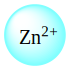
\includegraphics[width=0.1\textwidth]{C:/Users/emanuele/Desktop/PlacementEssay/PlacementEssay/backup/ChemspeedPlatformAllVersions/V12/Workflows/DataAnalysisWorkflow/FigureGeneration/chemicalDrawings/Zinc tetrafluoroborate.png}%
\end{minipage}%
\begin{minipage}{0.5\textwidth}%
\begin{center}%
\includegraphics[width=0.7\textwidth]{C:/Users/emanuele/Desktop/PlacementEssay/PlacementEssay/backup/ChemspeedPlatformAllVersions/V12/Workflows/DataAnalysisWorkflow/FigureGeneration/imagesForFigures/selfassemblyFailed.png}%
\end{center}%
\end{minipage}%
\caption{Self-assembly of components 8, 17, with Zinc(II) in a 3.0:1.5:1.0 molar ratio in CH$_3$CN at 60\textdegree C for 40h. These are the reagents (starting materials) for reaction 1.}%
\end{scheme}%
\begin{Decision Table}[H]%
\begin{tabular}{|c|c|c|c|}%
\hline%
&Human NMR Decision:&\multicolumn{2}{|c|}{NMR Spectra Category:}\\%
Human Reaction Decision:&Failed&\multicolumn{2}{|c|}{Oligomers formed.}\\%
\cline{2%
-%
4}%
Failed&Human MS Decision:&\multicolumn{2}{|c|}{MS Spectra Category:}\\%
&Failed&\multicolumn{2}{|c|}{Reaction occurred, unknown product.}\\%
\hline%
&&\multicolumn{2}{|c|}{NMR Criteria 1:}\\%
&Decision Maker NMR Decision:&\multicolumn{2}{|c|}{N/A}\\%
\cline{3%
-%
4}%
&N/A&\multicolumn{2}{|c|}{NMR Criteria 2:}\\%
Decision Maker Reaction Decision:&&\multicolumn{2}{|c|}{N/A}\\%
\cline{2%
-%
4}%
N/A&&MS Criteria 1 and 2:&Number of predicted peaks found in\\%
&Decision Maker MS Decision:&Failed&MS spectra with appropriate intensity:\\%
&Failed&&0\\%
\cline{3%
-%
4}%
&&MS Criteria 3:&Number of counter{-}ions found:\\%
&&Failed&0\\%
\hline%
\end{tabular}%
\caption{Human labled and Decsision maker labled outcomes for the \textsuperscript{1}H NMR spectroscopy and ULPC-MS spectrometry of reaction 1. Decision motivations are also given.}%
\end{Decision Table}%
\begin{NMR Spectra}[H]%
\begin{center}%
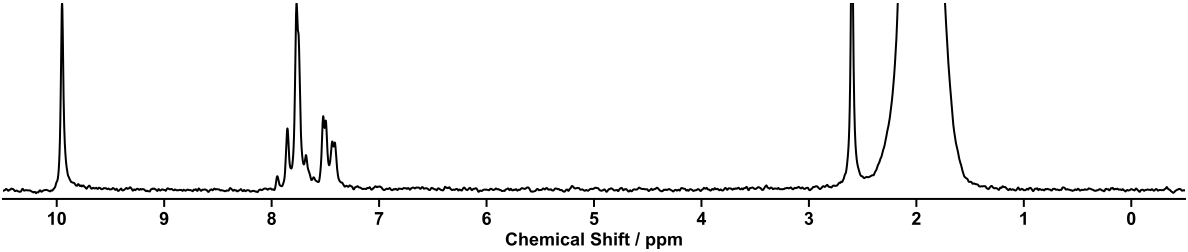
\includegraphics[width=1\textwidth]{C:/Users/emanuele/Desktop/PlacementEssay/PlacementEssay/backup/ChemspeedPlatformAllVersions/V12/Workflows/Data/StartingMaterials/ArchiveData/NMRreagentAnalysis-21.png}\hfill%
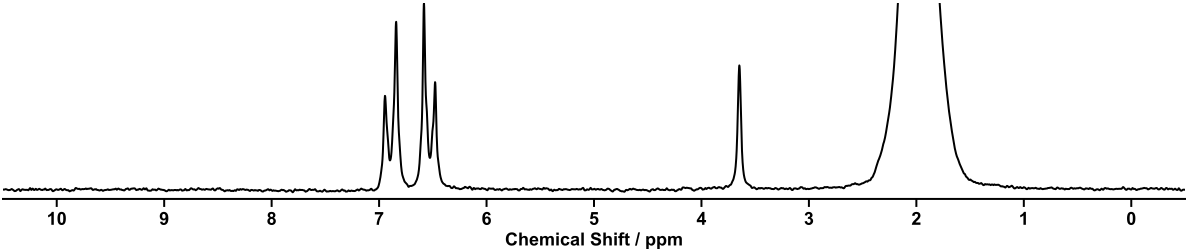
\includegraphics[width=1\textwidth]{C:/Users/emanuele/Desktop/PlacementEssay/PlacementEssay/backup/ChemspeedPlatformAllVersions/V12/Workflows/Data/StartingMaterials/ArchiveData/NMRreagentAnalysis-11.png}\hfill%
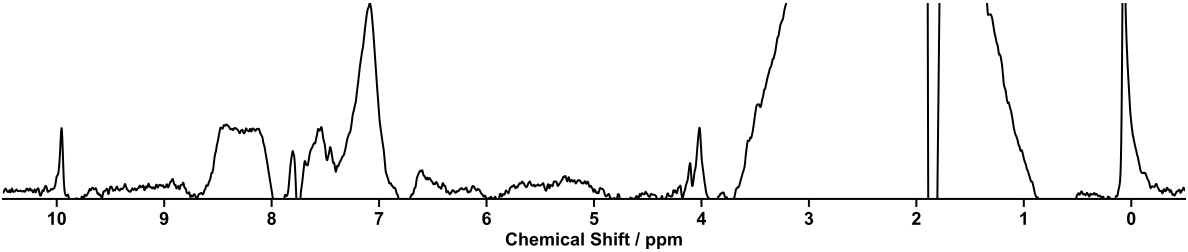
\includegraphics[width=1\textwidth]{C:/Users/emanuele/Desktop/PlacementEssay/PlacementEssay/backup/ChemspeedPlatformAllVersions/V12/Workflows/Data/Reactions/batch0/ArchiveData/NMR1.png}\hfill%
\end{center}%
\caption{The stacked \textsuperscript{1}H NMR spectra of the aldehyde (top), amine (middle), and reaction sample (bottom) for reaction 1.}%
\end{NMR Spectra}%
\begin{MS Spectra}[H]%
\begin{center}%
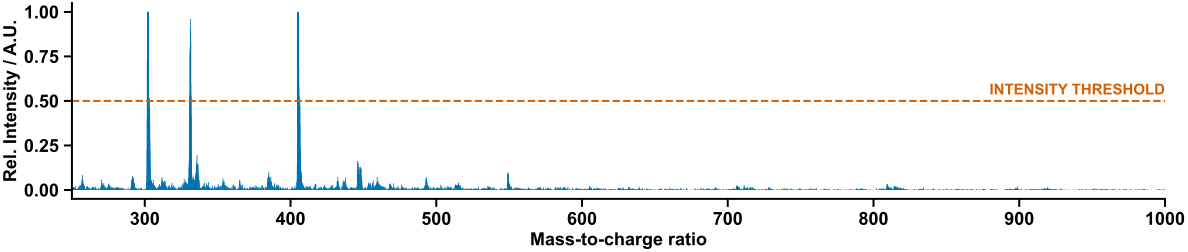
\includegraphics[width=1\textwidth]{C:/Users/emanuele/Desktop/PlacementEssay/PlacementEssay/backup/ChemspeedPlatformAllVersions/V12/Workflows/Data/Reactions/batch0/ArchiveData/MS1.png}\hfill%
\end{center}%
\caption{The ULPC-MS spectra of reaction 1. The intensity threshold is also shown.}%
\end{MS Spectra}%
\section*{Reaction 2}%
\addcontentsline{toc}{section}{\protect\numberline{}Reaction 2}%
\begin{scheme}[H]%
\begin{minipage}{0.5\textwidth}%

\includegraphics[width=0.4\textwidth]{C:/Users/emanuele/Desktop/PlacementEssay/PlacementEssay/backup/ChemspeedPlatformAllVersions/V12/Workflows/DataAnalysisWorkflow/FigureGeneration/chemicalDrawings/6-Methylpyridine-2-carboxaldehyde.png}%

\includegraphics[width=0.4\textwidth]{C:/Users/emanuele/Desktop/PlacementEssay/PlacementEssay/backup/ChemspeedPlatformAllVersions/V12/Workflows/DataAnalysisWorkflow/FigureGeneration/chemicalDrawings/2,2'-(Ethane-1,2-diylbis(oxy))diethanamine.png}%
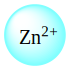
\includegraphics[width=0.1\textwidth]{C:/Users/emanuele/Desktop/PlacementEssay/PlacementEssay/backup/ChemspeedPlatformAllVersions/V12/Workflows/DataAnalysisWorkflow/FigureGeneration/chemicalDrawings/Zinc tetrafluoroborate.png}%
\end{minipage}%
\begin{minipage}{0.5\textwidth}%
\begin{center}%
\includegraphics[width=0.7\textwidth]{C:/Users/emanuele/Desktop/PlacementEssay/PlacementEssay/backup/ChemspeedPlatformAllVersions/V12/Workflows/DataAnalysisWorkflow/FigureGeneration/imagesForFigures/selfassemblyFailed.png}%
\end{center}%
\end{minipage}%
\caption{Self-assembly of components 8, 19, with Zinc(II) in a 3.0:1.5:1.0 molar ratio in CH$_3$CN at 60\textdegree C for 40h. These are the reagents (starting materials) for reaction 2.}%
\end{scheme}%
\begin{Decision Table}[H]%
\begin{tabular}{|c|c|c|c|}%
\hline%
&Human NMR Decision:&\multicolumn{2}{|c|}{NMR Spectra Category:}\\%
Human Reaction Decision:&Failed&\multicolumn{2}{|c|}{Oligomers formed.}\\%
\cline{2%
-%
4}%
Failed&Human MS Decision:&\multicolumn{2}{|c|}{MS Spectra Category:}\\%
&Failed&\multicolumn{2}{|c|}{Reaction failed.}\\%
\hline%
&&\multicolumn{2}{|c|}{NMR Criteria 1:}\\%
&Decision Maker NMR Decision:&\multicolumn{2}{|c|}{N/A}\\%
\cline{3%
-%
4}%
&N/A&\multicolumn{2}{|c|}{NMR Criteria 2:}\\%
Decision Maker Reaction Decision:&&\multicolumn{2}{|c|}{N/A}\\%
\cline{2%
-%
4}%
N/A&&MS Criteria 1 and 2:&Number of predicted peaks found in\\%
&Decision Maker MS Decision:&Failed&MS spectra with appropriate intensity:\\%
&Failed&&0\\%
\cline{3%
-%
4}%
&&MS Criteria 3:&Number of counter{-}ions found:\\%
&&Failed&0\\%
\hline%
\end{tabular}%
\caption{Human labled and Decsision maker labled outcomes for the \textsuperscript{1}H NMR spectroscopy and ULPC-MS spectrometry of reaction 2. Decision motivations are also given.}%
\end{Decision Table}%
\begin{NMR Spectra}[H]%
\begin{center}%
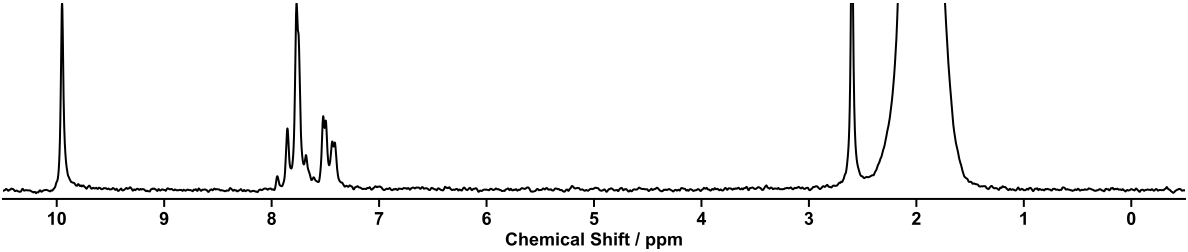
\includegraphics[width=1\textwidth]{C:/Users/emanuele/Desktop/PlacementEssay/PlacementEssay/backup/ChemspeedPlatformAllVersions/V12/Workflows/Data/StartingMaterials/ArchiveData/NMRreagentAnalysis-21.png}\hfill%
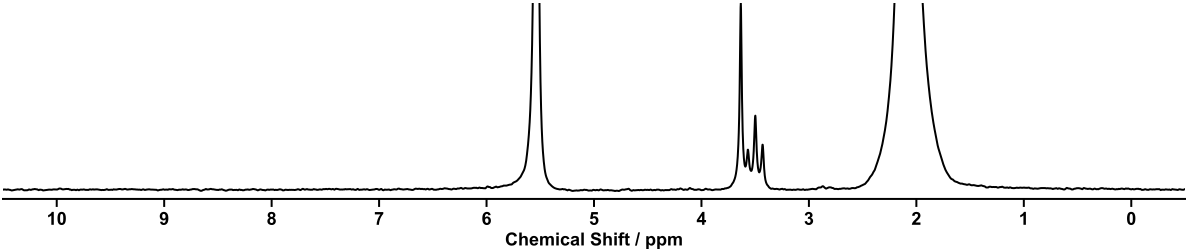
\includegraphics[width=1\textwidth]{C:/Users/emanuele/Desktop/PlacementEssay/PlacementEssay/backup/ChemspeedPlatformAllVersions/V12/Workflows/Data/StartingMaterials/ArchiveData/NMRreagentAnalysis-09.png}\hfill%
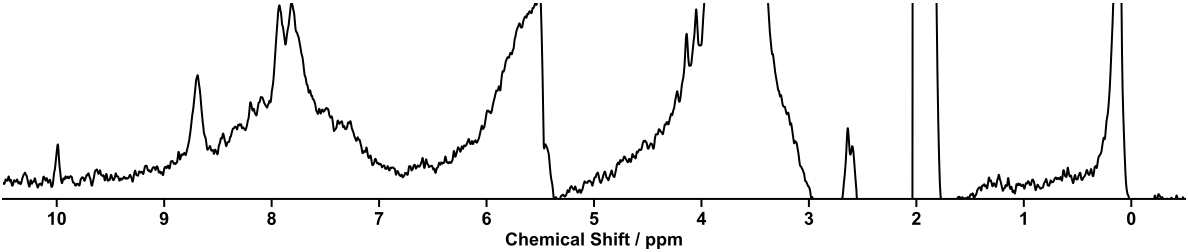
\includegraphics[width=1\textwidth]{C:/Users/emanuele/Desktop/PlacementEssay/PlacementEssay/backup/ChemspeedPlatformAllVersions/V12/Workflows/Data/Reactions/batch0/ArchiveData/NMR2.png}\hfill%
\end{center}%
\caption{The stacked \textsuperscript{1}H NMR spectra of the aldehyde (top), amine (middle), and reaction sample (bottom) for reaction 2.}%
\end{NMR Spectra}%
\begin{MS Spectra}[H]%
\begin{center}%
\includegraphics[width=1\textwidth]{C:/Users/emanuele/Desktop/PlacementEssay/PlacementEssay/backup/ChemspeedPlatformAllVersions/V12/Workflows/Data/Reactions/batch0/ArchiveData/MS2.png}\hfill%
\end{center}%
\caption{The ULPC-MS spectra of reaction 2. The intensity threshold is also shown.}%
\end{MS Spectra}%
\section*{Reaction 3}%
\addcontentsline{toc}{section}{\protect\numberline{}Reaction 3}%
\begin{scheme}[H]%
\begin{minipage}{0.5\textwidth}%

\includegraphics[width=0.4\textwidth]{C:/Users/emanuele/Desktop/PlacementEssay/PlacementEssay/backup/ChemspeedPlatformAllVersions/V12/Workflows/DataAnalysisWorkflow/FigureGeneration/chemicalDrawings/6-Methylpyridine-2-carboxaldehyde.png}%

\includegraphics[width=0.4\textwidth]{C:/Users/emanuele/Desktop/PlacementEssay/PlacementEssay/backup/ChemspeedPlatformAllVersions/V12/Workflows/DataAnalysisWorkflow/FigureGeneration/chemicalDrawings/4,4'-Oxydianiline.png}%
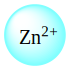
\includegraphics[width=0.1\textwidth]{C:/Users/emanuele/Desktop/PlacementEssay/PlacementEssay/backup/ChemspeedPlatformAllVersions/V12/Workflows/DataAnalysisWorkflow/FigureGeneration/chemicalDrawings/Zinc tetrafluoroborate.png}%
\end{minipage}%
\begin{minipage}{0.5\textwidth}%
\begin{center}%
\includegraphics[width=0.7\textwidth]{C:/Users/emanuele/Desktop/PlacementEssay/PlacementEssay/backup/ChemspeedPlatformAllVersions/V12/Workflows/DataAnalysisWorkflow/FigureGeneration/imagesForFigures/selfassemblyFailed.png}%
\end{center}%
\end{minipage}%
\caption{Self-assembly of components 8, 15, with Zinc(II) in a 3.0:1.5:1.0 molar ratio in CH$_3$CN at 60\textdegree C for 40h. These are the reagents (starting materials) for reaction 3.}%
\end{scheme}%
\begin{Decision Table}[H]%
\begin{tabular}{|c|c|c|c|}%
\hline%
&Human NMR Decision:&\multicolumn{2}{|c|}{NMR Spectra Category:}\\%
Human Reaction Decision:&Pass&\multicolumn{2}{|c|}{Single discrete species formed.}\\%
\cline{2%
-%
4}%
Failed&Human MS Decision:&\multicolumn{2}{|c|}{MS Spectra Category:}\\%
&Failed&\multicolumn{2}{|c|}{Reaction occurred, unknown product.}\\%
\hline%
&&\multicolumn{2}{|c|}{NMR Criteria 1:}\\%
&Decision Maker NMR Decision:&\multicolumn{2}{|c|}{N/A}\\%
\cline{3%
-%
4}%
&N/A&\multicolumn{2}{|c|}{NMR Criteria 2:}\\%
Decision Maker Reaction Decision:&&\multicolumn{2}{|c|}{N/A}\\%
\cline{2%
-%
4}%
N/A&&MS Criteria 1 and 2:&Number of predicted peaks found in\\%
&Decision Maker MS Decision:&Failed&MS spectra with appropriate intensity:\\%
&Failed&&0\\%
\cline{3%
-%
4}%
&&MS Criteria 3:&Number of counter{-}ions found:\\%
&&Failed&0\\%
\hline%
\end{tabular}%
\caption{Human labled and Decsision maker labled outcomes for the \textsuperscript{1}H NMR spectroscopy and ULPC-MS spectrometry of reaction 3. Decision motivations are also given.}%
\end{Decision Table}%
\begin{NMR Spectra}[H]%
\begin{center}%
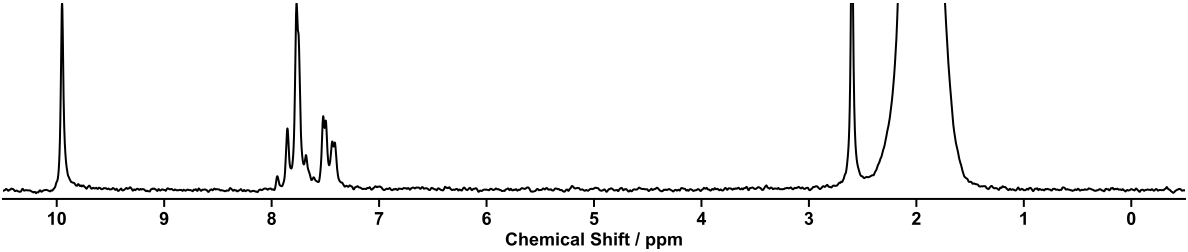
\includegraphics[width=1\textwidth]{C:/Users/emanuele/Desktop/PlacementEssay/PlacementEssay/backup/ChemspeedPlatformAllVersions/V12/Workflows/Data/StartingMaterials/ArchiveData/NMRreagentAnalysis-21.png}\hfill%
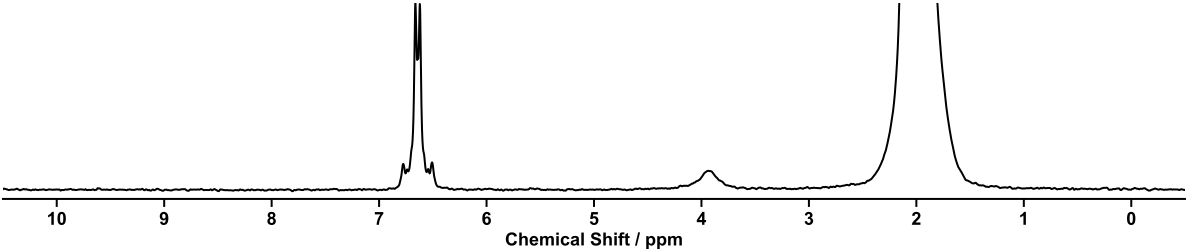
\includegraphics[width=1\textwidth]{C:/Users/emanuele/Desktop/PlacementEssay/PlacementEssay/backup/ChemspeedPlatformAllVersions/V12/Workflows/Data/StartingMaterials/ArchiveData/NMRreagentAnalysis-18.png}\hfill%
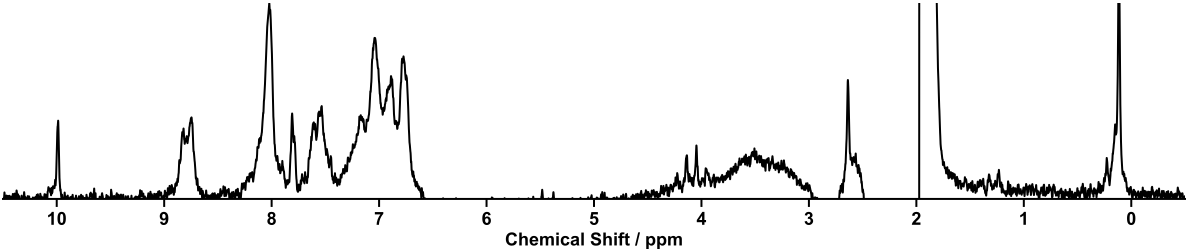
\includegraphics[width=1\textwidth]{C:/Users/emanuele/Desktop/PlacementEssay/PlacementEssay/backup/ChemspeedPlatformAllVersions/V12/Workflows/Data/Reactions/batch0/ArchiveData/NMR3.png}\hfill%
\end{center}%
\caption{The stacked \textsuperscript{1}H NMR spectra of the aldehyde (top), amine (middle), and reaction sample (bottom) for reaction 3.}%
\end{NMR Spectra}%
\begin{MS Spectra}[H]%
\begin{center}%
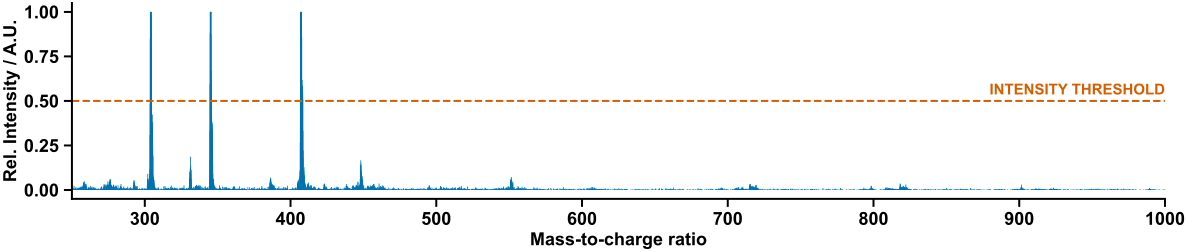
\includegraphics[width=1\textwidth]{C:/Users/emanuele/Desktop/PlacementEssay/PlacementEssay/backup/ChemspeedPlatformAllVersions/V12/Workflows/Data/Reactions/batch0/ArchiveData/MS3.png}\hfill%
\end{center}%
\caption{The ULPC-MS spectra of reaction 3. The intensity threshold is also shown.}%
\end{MS Spectra}%
\section*{Reaction 4}%
\addcontentsline{toc}{section}{\protect\numberline{}Reaction 4}%
\begin{scheme}[H]%
\begin{minipage}{0.5\textwidth}%

\includegraphics[width=0.4\textwidth]{C:/Users/emanuele/Desktop/PlacementEssay/PlacementEssay/backup/ChemspeedPlatformAllVersions/V12/Workflows/DataAnalysisWorkflow/FigureGeneration/chemicalDrawings/6-Methylpyridine-2-carboxaldehyde.png}%

\includegraphics[width=0.4\textwidth]{C:/Users/emanuele/Desktop/PlacementEssay/PlacementEssay/backup/ChemspeedPlatformAllVersions/V12/Workflows/DataAnalysisWorkflow/FigureGeneration/chemicalDrawings/4,4'-Methylenedianiline.png}%
\includegraphics[width=0.1\textwidth]{C:/Users/emanuele/Desktop/PlacementEssay/PlacementEssay/backup/ChemspeedPlatformAllVersions/V12/Workflows/DataAnalysisWorkflow/FigureGeneration/chemicalDrawings/Iron(II) tetrafluoroborate hexahydrate.png}%
\end{minipage}%
\begin{minipage}{0.5\textwidth}%
\begin{center}%
\includegraphics[width=0.7\textwidth]{C:/Users/emanuele/Desktop/PlacementEssay/PlacementEssay/backup/ChemspeedPlatformAllVersions/V12/Workflows/DataAnalysisWorkflow/FigureGeneration/imagesForFigures/selfassemblyFailed.png}%
\end{center}%
\end{minipage}%
\caption{Self-assembly of components 8, 17, with Iron(II) in a 3.0:1.5:1.0 molar ratio in CH$_3$CN at 60\textdegree C for 40h. These are the reagents (starting materials) for reaction 4.}%
\end{scheme}%
\begin{Decision Table}[H]%
\begin{tabular}{|c|c|c|c|}%
\hline%
&Human NMR Decision:&\multicolumn{2}{|c|}{NMR Spectra Category:}\\%
Human Reaction Decision:&ERROR&\multicolumn{2}{|c|}{Paramagnetic species formed.}\\%
\cline{2%
-%
4}%
Failed&Human MS Decision:&\multicolumn{2}{|c|}{MS Spectra Category:}\\%
&Failed&\multicolumn{2}{|c|}{Reaction occurred, unknown product.}\\%
\hline%
&&\multicolumn{2}{|c|}{NMR Criteria 1:}\\%
&Decision Maker NMR Decision:&\multicolumn{2}{|c|}{N/A}\\%
\cline{3%
-%
4}%
&N/A&\multicolumn{2}{|c|}{NMR Criteria 2:}\\%
Decision Maker Reaction Decision:&&\multicolumn{2}{|c|}{N/A}\\%
\cline{2%
-%
4}%
N/A&&MS Criteria 1 and 2:&Number of predicted peaks found in\\%
&Decision Maker MS Decision:&Pass&MS spectra with appropriate intensity:\\%
&Pass&&1\\%
\cline{3%
-%
4}%
&&MS Criteria 3:&Number of counter{-}ions found:\\%
&&Failed&0\\%
\hline%
\end{tabular}%
\caption{Human labled and Decsision maker labled outcomes for the \textsuperscript{1}H NMR spectroscopy and ULPC-MS spectrometry of reaction 4. Decision motivations are also given.}%
\end{Decision Table}%
\begin{NMR Spectra}[H]%
\begin{center}%
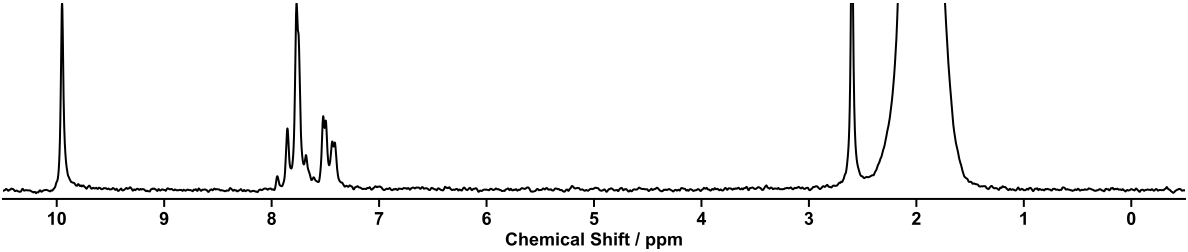
\includegraphics[width=1\textwidth]{C:/Users/emanuele/Desktop/PlacementEssay/PlacementEssay/backup/ChemspeedPlatformAllVersions/V12/Workflows/Data/StartingMaterials/ArchiveData/NMRreagentAnalysis-21.png}\hfill%
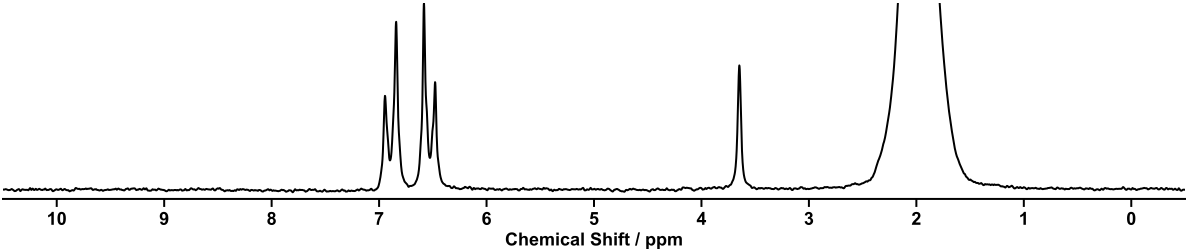
\includegraphics[width=1\textwidth]{C:/Users/emanuele/Desktop/PlacementEssay/PlacementEssay/backup/ChemspeedPlatformAllVersions/V12/Workflows/Data/StartingMaterials/ArchiveData/NMRreagentAnalysis-11.png}\hfill%
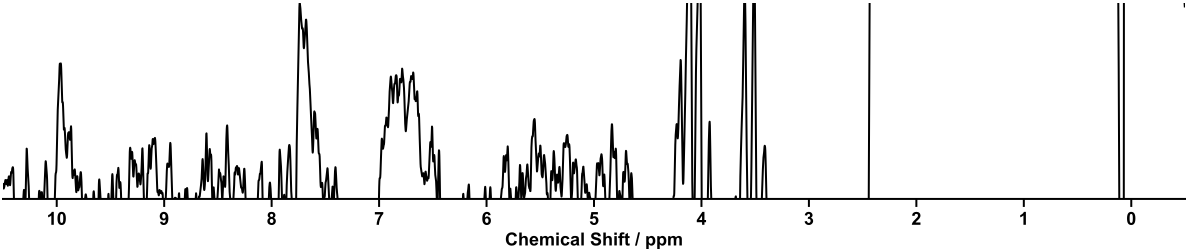
\includegraphics[width=1\textwidth]{C:/Users/emanuele/Desktop/PlacementEssay/PlacementEssay/backup/ChemspeedPlatformAllVersions/V12/Workflows/Data/Reactions/batch0/ArchiveData/NMR4.png}\hfill%
\end{center}%
\caption{The stacked \textsuperscript{1}H NMR spectra of the aldehyde (top), amine (middle), and reaction sample (bottom) for reaction 4.}%
\end{NMR Spectra}%
\begin{MS Spectra}[H]%
\begin{center}%
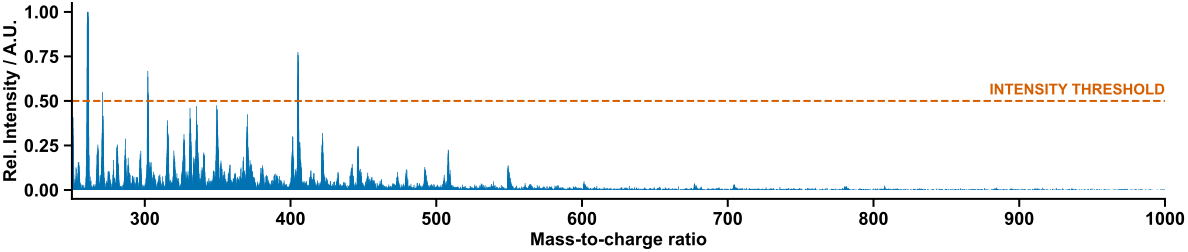
\includegraphics[width=1\textwidth]{C:/Users/emanuele/Desktop/PlacementEssay/PlacementEssay/backup/ChemspeedPlatformAllVersions/V12/Workflows/Data/Reactions/batch0/ArchiveData/MS4.png}\hfill%
\end{center}%
\caption{The ULPC-MS spectra of reaction 4. The intensity threshold is also shown.}%
\end{MS Spectra}%
\section*{Reaction 5}%
\addcontentsline{toc}{section}{\protect\numberline{}Reaction 5}%
\begin{scheme}[H]%
\begin{minipage}{0.5\textwidth}%

\includegraphics[width=0.4\textwidth]{C:/Users/emanuele/Desktop/PlacementEssay/PlacementEssay/backup/ChemspeedPlatformAllVersions/V12/Workflows/DataAnalysisWorkflow/FigureGeneration/chemicalDrawings/6-Methylpyridine-2-carboxaldehyde.png}%

\includegraphics[width=0.4\textwidth]{C:/Users/emanuele/Desktop/PlacementEssay/PlacementEssay/backup/ChemspeedPlatformAllVersions/V12/Workflows/DataAnalysisWorkflow/FigureGeneration/chemicalDrawings/2,2'-(Ethane-1,2-diylbis(oxy))diethanamine.png}%
\includegraphics[width=0.1\textwidth]{C:/Users/emanuele/Desktop/PlacementEssay/PlacementEssay/backup/ChemspeedPlatformAllVersions/V12/Workflows/DataAnalysisWorkflow/FigureGeneration/chemicalDrawings/Iron(II) tetrafluoroborate hexahydrate.png}%
\end{minipage}%
\begin{minipage}{0.5\textwidth}%
\begin{center}%
\includegraphics[width=0.7\textwidth]{C:/Users/emanuele/Desktop/PlacementEssay/PlacementEssay/backup/ChemspeedPlatformAllVersions/V12/Workflows/DataAnalysisWorkflow/FigureGeneration/imagesForFigures/selfassemblyFailed.png}%
\end{center}%
\end{minipage}%
\caption{Self-assembly of components 8, 19, with Iron(II) in a 3.0:1.5:1.0 molar ratio in CH$_3$CN at 60\textdegree C for 40h. These are the reagents (starting materials) for reaction 5.}%
\end{scheme}%
\begin{Decision Table}[H]%
\begin{tabular}{|c|c|c|c|}%
\hline%
&Human NMR Decision:&\multicolumn{2}{|c|}{NMR Spectra Category:}\\%
Human Reaction Decision:&Failed&\multicolumn{2}{|c|}{No reaction occured.}\\%
\cline{2%
-%
4}%
Failed&Human MS Decision:&\multicolumn{2}{|c|}{MS Spectra Category:}\\%
&Failed&\multicolumn{2}{|c|}{Reaction failed.}\\%
\hline%
&&\multicolumn{2}{|c|}{NMR Criteria 1:}\\%
&Decision Maker NMR Decision:&\multicolumn{2}{|c|}{N/A}\\%
\cline{3%
-%
4}%
&N/A&\multicolumn{2}{|c|}{NMR Criteria 2:}\\%
Decision Maker Reaction Decision:&&\multicolumn{2}{|c|}{N/A}\\%
\cline{2%
-%
4}%
N/A&&MS Criteria 1 and 2:&Number of predicted peaks found in\\%
&Decision Maker MS Decision:&Failed&MS spectra with appropriate intensity:\\%
&Failed&&0\\%
\cline{3%
-%
4}%
&&MS Criteria 3:&Number of counter{-}ions found:\\%
&&Failed&0\\%
\hline%
\end{tabular}%
\caption{Human labled and Decsision maker labled outcomes for the \textsuperscript{1}H NMR spectroscopy and ULPC-MS spectrometry of reaction 5. Decision motivations are also given.}%
\end{Decision Table}%
\begin{NMR Spectra}[H]%
\begin{center}%
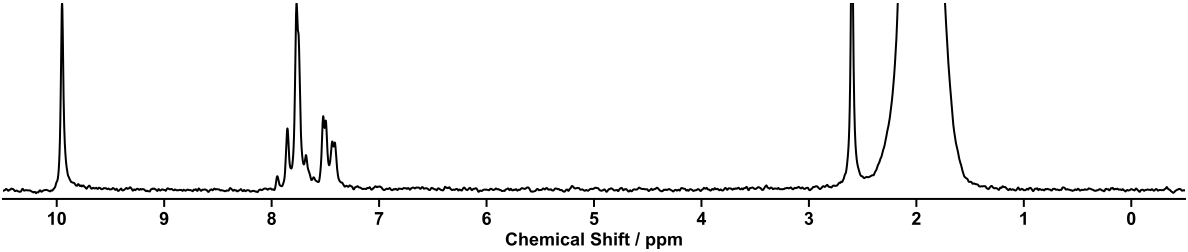
\includegraphics[width=1\textwidth]{C:/Users/emanuele/Desktop/PlacementEssay/PlacementEssay/backup/ChemspeedPlatformAllVersions/V12/Workflows/Data/StartingMaterials/ArchiveData/NMRreagentAnalysis-21.png}\hfill%
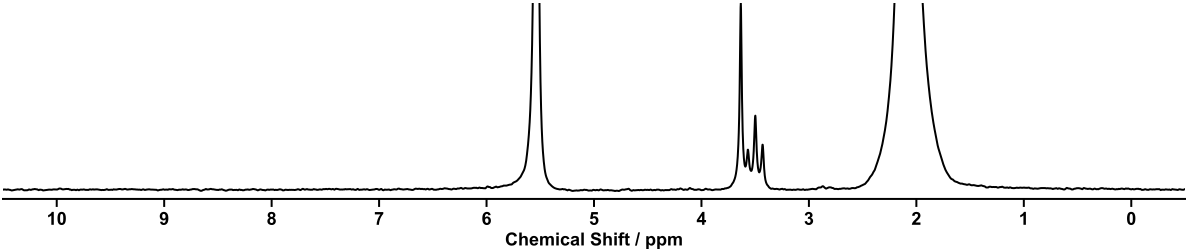
\includegraphics[width=1\textwidth]{C:/Users/emanuele/Desktop/PlacementEssay/PlacementEssay/backup/ChemspeedPlatformAllVersions/V12/Workflows/Data/StartingMaterials/ArchiveData/NMRreagentAnalysis-09.png}\hfill%
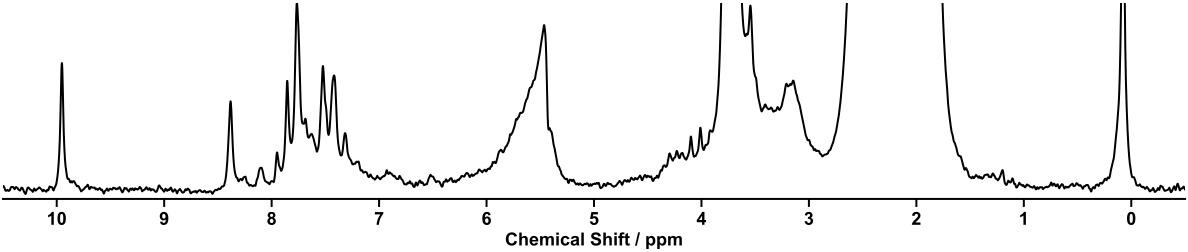
\includegraphics[width=1\textwidth]{C:/Users/emanuele/Desktop/PlacementEssay/PlacementEssay/backup/ChemspeedPlatformAllVersions/V12/Workflows/Data/Reactions/batch0/ArchiveData/NMR5.png}\hfill%
\end{center}%
\caption{The stacked \textsuperscript{1}H NMR spectra of the aldehyde (top), amine (middle), and reaction sample (bottom) for reaction 5.}%
\end{NMR Spectra}%
\begin{MS Spectra}[H]%
\begin{center}%
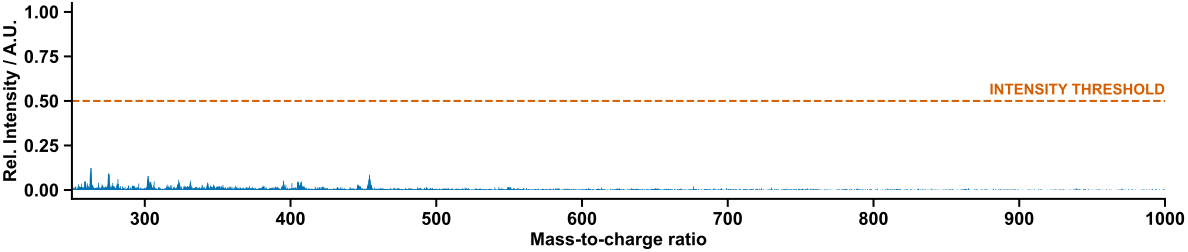
\includegraphics[width=1\textwidth]{C:/Users/emanuele/Desktop/PlacementEssay/PlacementEssay/backup/ChemspeedPlatformAllVersions/V12/Workflows/Data/Reactions/batch0/ArchiveData/MS5.png}\hfill%
\end{center}%
\caption{The ULPC-MS spectra of reaction 5. The intensity threshold is also shown.}%
\end{MS Spectra}%
\section*{Reaction 7}%
\addcontentsline{toc}{section}{\protect\numberline{}Reaction 7}%
\begin{scheme}[H]%
\begin{minipage}{0.5\textwidth}%
\includegraphics[width=0.4\textwidth]{C:/Users/emanuele/Desktop/PlacementEssay/PlacementEssay/backup/ChemspeedPlatformAllVersions/V12/Workflows/DataAnalysisWorkflow/FigureGeneration/chemicalDrawings/6-Methoxypyridine-2-carbaldehyde.png}%

\includegraphics[width=0.4\textwidth]{C:/Users/emanuele/Desktop/PlacementEssay/PlacementEssay/backup/ChemspeedPlatformAllVersions/V12/Workflows/DataAnalysisWorkflow/FigureGeneration/chemicalDrawings/4,4'-Methylenedianiline.png}%
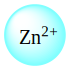
\includegraphics[width=0.1\textwidth]{C:/Users/emanuele/Desktop/PlacementEssay/PlacementEssay/backup/ChemspeedPlatformAllVersions/V12/Workflows/DataAnalysisWorkflow/FigureGeneration/chemicalDrawings/Zinc tetrafluoroborate.png}%
\end{minipage}%
\begin{minipage}{0.5\textwidth}%
\begin{center}%
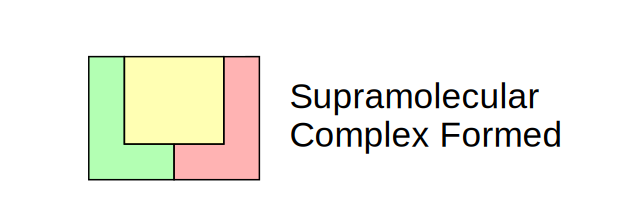
\includegraphics[width=0.7\textwidth]{C:/Users/emanuele/Desktop/PlacementEssay/PlacementEssay/backup/ChemspeedPlatformAllVersions/V12/Workflows/DataAnalysisWorkflow/FigureGeneration/imagesForFigures/selfassemblySuccessful.png}%
\end{center}%
\end{minipage}%
\caption{Self-assembly of components 6, 17, with Zinc(II) in a 3.0:1.5:1.0 molar ratio in CH$_3$CN at 60\textdegree C for 40h. These are the reagents (starting materials) for reaction 7.}%
\end{scheme}%
\begin{Decision Table}[H]%
\begin{tabular}{|c|c|c|c|}%
\hline%
&Human NMR Decision:&\multicolumn{2}{|c|}{NMR Spectra Category:}\\%
Human Reaction Decision:&Pass&\multicolumn{2}{|c|}{Single discrete species formed.}\\%
\cline{2%
-%
4}%
Pass&Human MS Decision:&\multicolumn{2}{|c|}{MS Spectra Category:}\\%
&Pass&\multicolumn{2}{|c|}{Reaction occurred, supramolecular product.}\\%
\hline%
&&\multicolumn{2}{|c|}{NMR Criteria 1:}\\%
&Decision Maker NMR Decision:&\multicolumn{2}{|c|}{N/A}\\%
\cline{3%
-%
4}%
&N/A&\multicolumn{2}{|c|}{NMR Criteria 2:}\\%
Decision Maker Reaction Decision:&&\multicolumn{2}{|c|}{N/A}\\%
\cline{2%
-%
4}%
N/A&&MS Criteria 1 and 2:&Number of predicted peaks found in\\%
&Decision Maker MS Decision:&Pass&MS spectra with appropriate intensity:\\%
&Pass&&5\\%
\cline{3%
-%
4}%
&&MS Criteria 3:&Number of counter{-}ions found:\\%
&&Pass&4\\%
\hline%
\end{tabular}%
\caption{Human labled and Decsision maker labled outcomes for the \textsuperscript{1}H NMR spectroscopy and ULPC-MS spectrometry of reaction 7. Decision motivations are also given.}%
\end{Decision Table}%
\begin{NMR Spectra}[H]%
\begin{center}%
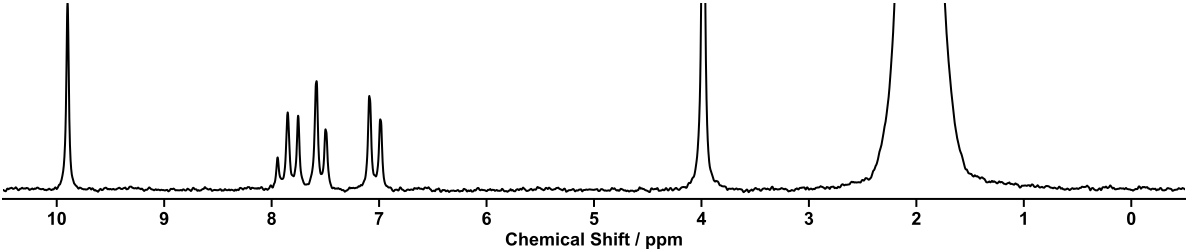
\includegraphics[width=1\textwidth]{C:/Users/emanuele/Desktop/PlacementEssay/PlacementEssay/backup/ChemspeedPlatformAllVersions/V12/Workflows/Data/StartingMaterials/ArchiveData/NMRreagentAnalysis-29.png}\hfill%
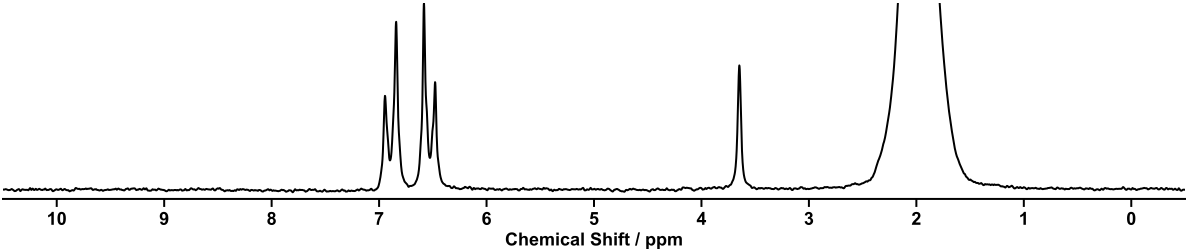
\includegraphics[width=1\textwidth]{C:/Users/emanuele/Desktop/PlacementEssay/PlacementEssay/backup/ChemspeedPlatformAllVersions/V12/Workflows/Data/StartingMaterials/ArchiveData/NMRreagentAnalysis-11.png}\hfill%
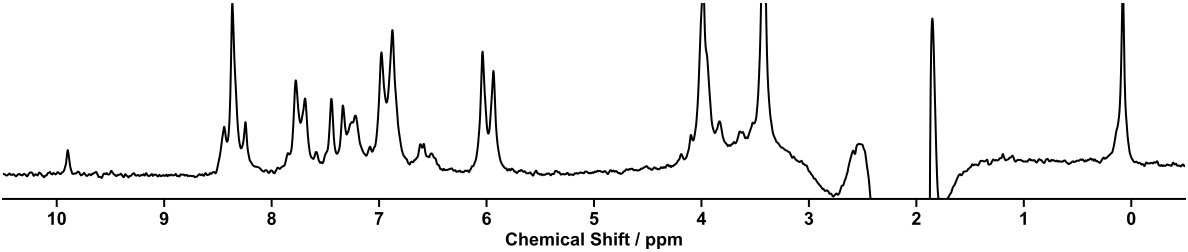
\includegraphics[width=1\textwidth]{C:/Users/emanuele/Desktop/PlacementEssay/PlacementEssay/backup/ChemspeedPlatformAllVersions/V12/Workflows/Data/Reactions/batch0/ArchiveData/NMR7.png}\hfill%
\end{center}%
\caption{The stacked \textsuperscript{1}H NMR spectra of the aldehyde (top), amine (middle), and reaction sample (bottom) for reaction 7.}%
\end{NMR Spectra}%
\begin{MS Spectra}[H]%
\begin{center}%
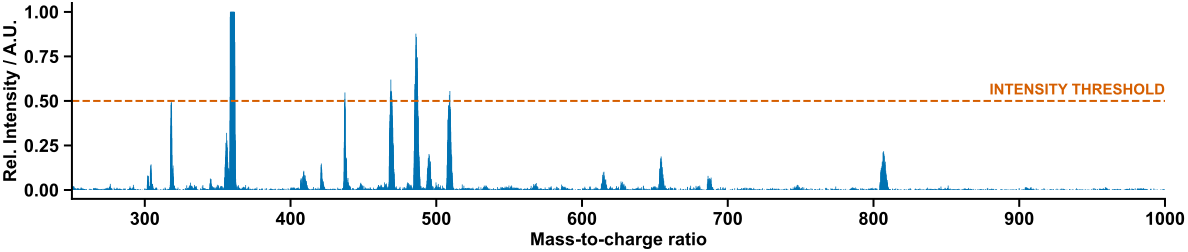
\includegraphics[width=1\textwidth]{C:/Users/emanuele/Desktop/PlacementEssay/PlacementEssay/backup/ChemspeedPlatformAllVersions/V12/Workflows/Data/Reactions/batch0/ArchiveData/MS7.png}\hfill%
\end{center}%
\caption{The ULPC-MS spectra of reaction 7. The intensity threshold is also shown.}%
\end{MS Spectra}%
\section*{Reaction 8}%
\addcontentsline{toc}{section}{\protect\numberline{}Reaction 8}%
\begin{scheme}[H]%
\begin{minipage}{0.5\textwidth}%
\includegraphics[width=0.4\textwidth]{C:/Users/emanuele/Desktop/PlacementEssay/PlacementEssay/backup/ChemspeedPlatformAllVersions/V12/Workflows/DataAnalysisWorkflow/FigureGeneration/chemicalDrawings/6-Methoxypyridine-2-carbaldehyde.png}%

\includegraphics[width=0.4\textwidth]{C:/Users/emanuele/Desktop/PlacementEssay/PlacementEssay/backup/ChemspeedPlatformAllVersions/V12/Workflows/DataAnalysisWorkflow/FigureGeneration/chemicalDrawings/2,2'-(Ethane-1,2-diylbis(oxy))diethanamine.png}%
\includegraphics[width=0.1\textwidth]{C:/Users/emanuele/Desktop/PlacementEssay/PlacementEssay/backup/ChemspeedPlatformAllVersions/V12/Workflows/DataAnalysisWorkflow/FigureGeneration/chemicalDrawings/Zinc tetrafluoroborate.png}%
\end{minipage}%
\begin{minipage}{0.5\textwidth}%
\begin{center}%
\includegraphics[width=0.7\textwidth]{C:/Users/emanuele/Desktop/PlacementEssay/PlacementEssay/backup/ChemspeedPlatformAllVersions/V12/Workflows/DataAnalysisWorkflow/FigureGeneration/imagesForFigures/selfassemblyFailed.png}%
\end{center}%
\end{minipage}%
\caption{Self-assembly of components 6, 19, with Zinc(II) in a 3.0:1.5:1.0 molar ratio in CH$_3$CN at 60\textdegree C for 40h. These are the reagents (starting materials) for reaction 8.}%
\end{scheme}%
\begin{Decision Table}[H]%
\begin{tabular}{|c|c|c|c|}%
\hline%
&Human NMR Decision:&\multicolumn{2}{|c|}{NMR Spectra Category:}\\%
Human Reaction Decision:&Failed&\multicolumn{2}{|c|}{Oligomers formed.}\\%
\cline{2%
-%
4}%
Failed&Human MS Decision:&\multicolumn{2}{|c|}{MS Spectra Category:}\\%
&Failed&\multicolumn{2}{|c|}{Reaction failed.}\\%
\hline%
&&\multicolumn{2}{|c|}{NMR Criteria 1:}\\%
&Decision Maker NMR Decision:&\multicolumn{2}{|c|}{N/A}\\%
\cline{3%
-%
4}%
&N/A&\multicolumn{2}{|c|}{NMR Criteria 2:}\\%
Decision Maker Reaction Decision:&&\multicolumn{2}{|c|}{N/A}\\%
\cline{2%
-%
4}%
N/A&&MS Criteria 1 and 2:&Number of predicted peaks found in\\%
&Decision Maker MS Decision:&Failed&MS spectra with appropriate intensity:\\%
&Failed&&0\\%
\cline{3%
-%
4}%
&&MS Criteria 3:&Number of counter{-}ions found:\\%
&&Failed&0\\%
\hline%
\end{tabular}%
\caption{Human labled and Decsision maker labled outcomes for the \textsuperscript{1}H NMR spectroscopy and ULPC-MS spectrometry of reaction 8. Decision motivations are also given.}%
\end{Decision Table}%
\begin{NMR Spectra}[H]%
\begin{center}%
\includegraphics[width=1\textwidth]{C:/Users/emanuele/Desktop/PlacementEssay/PlacementEssay/backup/ChemspeedPlatformAllVersions/V12/Workflows/Data/StartingMaterials/ArchiveData/NMRreagentAnalysis-29.png}\hfill%
\includegraphics[width=1\textwidth]{C:/Users/emanuele/Desktop/PlacementEssay/PlacementEssay/backup/ChemspeedPlatformAllVersions/V12/Workflows/Data/StartingMaterials/ArchiveData/NMRreagentAnalysis-09.png}\hfill%
\includegraphics[width=1\textwidth]{C:/Users/emanuele/Desktop/PlacementEssay/PlacementEssay/backup/ChemspeedPlatformAllVersions/V12/Workflows/Data/Reactions/batch0/ArchiveData/NMR8.png}\hfill%
\end{center}%
\caption{The stacked \textsuperscript{1}H NMR spectra of the aldehyde (top), amine (middle), and reaction sample (bottom) for reaction 8.}%
\end{NMR Spectra}%
\begin{MS Spectra}[H]%
\begin{center}%
\includegraphics[width=1\textwidth]{C:/Users/emanuele/Desktop/PlacementEssay/PlacementEssay/backup/ChemspeedPlatformAllVersions/V12/Workflows/Data/Reactions/batch0/ArchiveData/MS8.png}\hfill%
\end{center}%
\caption{The ULPC-MS spectra of reaction 8. The intensity threshold is also shown.}%
\end{MS Spectra}%
\section*{Reaction 9}%
\addcontentsline{toc}{section}{\protect\numberline{}Reaction 9}%
\begin{scheme}[H]%
\begin{minipage}{0.5\textwidth}%
\includegraphics[width=0.4\textwidth]{C:/Users/emanuele/Desktop/PlacementEssay/PlacementEssay/backup/ChemspeedPlatformAllVersions/V12/Workflows/DataAnalysisWorkflow/FigureGeneration/chemicalDrawings/6-Methoxypyridine-2-carbaldehyde.png}%
\includegraphics[width=0.4\textwidth]{C:/Users/emanuele/Desktop/PlacementEssay/PlacementEssay/backup/ChemspeedPlatformAllVersions/V12/Workflows/DataAnalysisWorkflow/FigureGeneration/chemicalDrawings/4,4'-Oxydianiline.png}%
\includegraphics[width=0.1\textwidth]{C:/Users/emanuele/Desktop/PlacementEssay/PlacementEssay/backup/ChemspeedPlatformAllVersions/V12/Workflows/DataAnalysisWorkflow/FigureGeneration/chemicalDrawings/Zinc tetrafluoroborate.png}%
\end{minipage}%
\begin{minipage}{0.5\textwidth}%
\begin{center}%
\includegraphics[width=0.7\textwidth]{C:/Users/emanuele/Desktop/PlacementEssay/PlacementEssay/backup/ChemspeedPlatformAllVersions/V12/Workflows/DataAnalysisWorkflow/FigureGeneration/imagesForFigures/selfassemblySuccessful.png}%
\end{center}%
\end{minipage}%
\caption{Self-assembly of components 6, 15, with Zinc(II) in a 3.0:1.5:1.0 molar ratio in CH$_3$CN at 60\textdegree C for 40h. These are the reagents (starting materials) for reaction 9.}%
\end{scheme}%
\begin{Decision Table}[H]%
\begin{tabular}{|c|c|c|c|}%
\hline%
&Human NMR Decision:&\multicolumn{2}{|c|}{NMR Spectra Category:}\\%
Human Reaction Decision:&Pass&\multicolumn{2}{|c|}{Single discrete species formed.}\\%
\cline{2%
-%
4}%
Pass&Human MS Decision:&\multicolumn{2}{|c|}{MS Spectra Category:}\\%
&Pass&\multicolumn{2}{|c|}{Reaction occurred, supramolecular product.}\\%
\hline%
&&\multicolumn{2}{|c|}{NMR Criteria 1:}\\%
&Decision Maker NMR Decision:&\multicolumn{2}{|c|}{N/A}\\%
\cline{3%
-%
4}%
&N/A&\multicolumn{2}{|c|}{NMR Criteria 2:}\\%
Decision Maker Reaction Decision:&&\multicolumn{2}{|c|}{N/A}\\%
\cline{2%
-%
4}%
N/A&&MS Criteria 1 and 2:&Number of predicted peaks found in\\%
&Decision Maker MS Decision:&Pass&MS spectra with appropriate intensity:\\%
&Pass&&2\\%
\cline{3%
-%
4}%
&&MS Criteria 3:&Number of counter{-}ions found:\\%
&&Pass&2\\%
\hline%
\end{tabular}%
\caption{Human labled and Decsision maker labled outcomes for the \textsuperscript{1}H NMR spectroscopy and ULPC-MS spectrometry of reaction 9. Decision motivations are also given.}%
\end{Decision Table}%
\begin{NMR Spectra}[H]%
\begin{center}%
\includegraphics[width=1\textwidth]{C:/Users/emanuele/Desktop/PlacementEssay/PlacementEssay/backup/ChemspeedPlatformAllVersions/V12/Workflows/Data/StartingMaterials/ArchiveData/NMRreagentAnalysis-29.png}\hfill%
\includegraphics[width=1\textwidth]{C:/Users/emanuele/Desktop/PlacementEssay/PlacementEssay/backup/ChemspeedPlatformAllVersions/V12/Workflows/Data/StartingMaterials/ArchiveData/NMRreagentAnalysis-18.png}\hfill%
\includegraphics[width=1\textwidth]{C:/Users/emanuele/Desktop/PlacementEssay/PlacementEssay/backup/ChemspeedPlatformAllVersions/V12/Workflows/Data/Reactions/batch0/ArchiveData/NMR9.png}\hfill%
\end{center}%
\caption{The stacked \textsuperscript{1}H NMR spectra of the aldehyde (top), amine (middle), and reaction sample (bottom) for reaction 9.}%
\end{NMR Spectra}%
\begin{MS Spectra}[H]%
\begin{center}%
\includegraphics[width=1\textwidth]{C:/Users/emanuele/Desktop/PlacementEssay/PlacementEssay/backup/ChemspeedPlatformAllVersions/V12/Workflows/Data/Reactions/batch0/ArchiveData/MS9.png}\hfill%
\end{center}%
\caption{The ULPC-MS spectra of reaction 9. The intensity threshold is also shown.}%
\end{MS Spectra}%
\section*{Reaction 10}%
\addcontentsline{toc}{section}{\protect\numberline{}Reaction 10}%
\begin{scheme}[H]%
\begin{minipage}{0.5\textwidth}%
\includegraphics[width=0.4\textwidth]{C:/Users/emanuele/Desktop/PlacementEssay/PlacementEssay/backup/ChemspeedPlatformAllVersions/V12/Workflows/DataAnalysisWorkflow/FigureGeneration/chemicalDrawings/6-Methylpyridine-2-carboxaldehyde.png}%
\includegraphics[width=0.4\textwidth]{C:/Users/emanuele/Desktop/PlacementEssay/PlacementEssay/backup/ChemspeedPlatformAllVersions/V12/Workflows/DataAnalysisWorkflow/FigureGeneration/chemicalDrawings/Naphthalene-1,8-diamine.png}%
\includegraphics[width=0.1\textwidth]{C:/Users/emanuele/Desktop/PlacementEssay/PlacementEssay/backup/ChemspeedPlatformAllVersions/V12/Workflows/DataAnalysisWorkflow/FigureGeneration/chemicalDrawings/Zinc tetrafluoroborate.png}%
\end{minipage}%
\begin{minipage}{0.5\textwidth}%
\begin{center}%
\includegraphics[width=0.7\textwidth]{C:/Users/emanuele/Desktop/PlacementEssay/PlacementEssay/backup/ChemspeedPlatformAllVersions/V12/Workflows/DataAnalysisWorkflow/FigureGeneration/imagesForFigures/selfassemblyFailed.png}%
\end{center}%
\end{minipage}%
\caption{Self-assembly of components 8, 21, with Zinc(II) in a 3.0:1.5:1.0 molar ratio in CH$_3$CN at 60\textdegree C for 40h. These are the reagents (starting materials) for reaction 10.}%
\end{scheme}%
\begin{Decision Table}[H]%
\begin{tabular}{|c|c|c|c|}%
\hline%
&Human NMR Decision:&\multicolumn{2}{|c|}{NMR Spectra Category:}\\%
Human Reaction Decision:&Failed&\multicolumn{2}{|c|}{Oligomers formed.}\\%
\cline{2%
-%
4}%
Failed&Human MS Decision:&\multicolumn{2}{|c|}{MS Spectra Category:}\\%
&Failed&\multicolumn{2}{|c|}{Reaction failed.}\\%
\hline%
&&\multicolumn{2}{|c|}{NMR Criteria 1:}\\%
&Decision Maker NMR Decision:&\multicolumn{2}{|c|}{N/A}\\%
\cline{3%
-%
4}%
&N/A&\multicolumn{2}{|c|}{NMR Criteria 2:}\\%
Decision Maker Reaction Decision:&&\multicolumn{2}{|c|}{N/A}\\%
\cline{2%
-%
4}%
N/A&&MS Criteria 1 and 2:&Number of predicted peaks found in\\%
&Decision Maker MS Decision:&Failed&MS spectra with appropriate intensity:\\%
&Failed&&0\\%
\cline{3%
-%
4}%
&&MS Criteria 3:&Number of counter{-}ions found:\\%
&&Failed&0\\%
\hline%
\end{tabular}%
\caption{Human labled and Decsision maker labled outcomes for the \textsuperscript{1}H NMR spectroscopy and ULPC-MS spectrometry of reaction 10. Decision motivations are also given.}%
\end{Decision Table}%
\begin{NMR Spectra}[H]%
\begin{center}%
\includegraphics[width=1\textwidth]{C:/Users/emanuele/Desktop/PlacementEssay/PlacementEssay/backup/ChemspeedPlatformAllVersions/V12/Workflows/Data/StartingMaterials/ArchiveData/NMRreagentAnalysis-21.png}\hfill%
\includegraphics[width=1\textwidth]{C:/Users/emanuele/Desktop/PlacementEssay/PlacementEssay/backup/ChemspeedPlatformAllVersions/V12/Workflows/Data/StartingMaterials/ArchiveData/NMRreagentAnalysis-17.png}\hfill%
\includegraphics[width=1\textwidth]{C:/Users/emanuele/Desktop/PlacementEssay/PlacementEssay/backup/ChemspeedPlatformAllVersions/V12/Workflows/Data/Reactions/batch0/ArchiveData/NMR10.png}\hfill%
\end{center}%
\caption{The stacked \textsuperscript{1}H NMR spectra of the aldehyde (top), amine (middle), and reaction sample (bottom) for reaction 10.}%
\end{NMR Spectra}%
\begin{MS Spectra}[H]%
\begin{center}%
\includegraphics[width=1\textwidth]{C:/Users/emanuele/Desktop/PlacementEssay/PlacementEssay/backup/ChemspeedPlatformAllVersions/V12/Workflows/Data/Reactions/batch0/ArchiveData/MS10.png}\hfill%
\end{center}%
\caption{The ULPC-MS spectra of reaction 10. The intensity threshold is also shown.}%
\end{MS Spectra}%
\section*{Reaction 11}%
\addcontentsline{toc}{section}{\protect\numberline{}Reaction 11}%
\begin{scheme}[H]%
\begin{minipage}{0.5\textwidth}%
\includegraphics[width=0.4\textwidth]{C:/Users/emanuele/Desktop/PlacementEssay/PlacementEssay/backup/ChemspeedPlatformAllVersions/V12/Workflows/DataAnalysisWorkflow/FigureGeneration/chemicalDrawings/6-Methylpyridine-2-carboxaldehyde.png}%
\includegraphics[width=0.4\textwidth]{C:/Users/emanuele/Desktop/PlacementEssay/PlacementEssay/backup/ChemspeedPlatformAllVersions/V12/Workflows/DataAnalysisWorkflow/FigureGeneration/chemicalDrawings/4,4'-(9H-AdamantaeFlurene-9,9diyl)dianiline.png}%
\includegraphics[width=0.1\textwidth]{C:/Users/emanuele/Desktop/PlacementEssay/PlacementEssay/backup/ChemspeedPlatformAllVersions/V12/Workflows/DataAnalysisWorkflow/FigureGeneration/chemicalDrawings/Zinc tetrafluoroborate.png}%
\end{minipage}%
\begin{minipage}{0.5\textwidth}%
\begin{center}%
\includegraphics[width=0.7\textwidth]{C:/Users/emanuele/Desktop/PlacementEssay/PlacementEssay/backup/ChemspeedPlatformAllVersions/V12/Workflows/DataAnalysisWorkflow/FigureGeneration/imagesForFigures/selfassemblySuccessful.png}%
\end{center}%
\end{minipage}%
\caption{Self-assembly of components 8, 13, with Zinc(II) in a 3.0:1.5:1.0 molar ratio in CH$_3$CN at 60\textdegree C for 40h. These are the reagents (starting materials) for reaction 11.}%
\end{scheme}%
\begin{Decision Table}[H]%
\begin{tabular}{|c|c|c|c|}%
\hline%
&Human NMR Decision:&\multicolumn{2}{|c|}{NMR Spectra Category:}\\%
Human Reaction Decision:&Pass&\multicolumn{2}{|c|}{Single discrete species formed.}\\%
\cline{2%
-%
4}%
Pass&Human MS Decision:&\multicolumn{2}{|c|}{MS Spectra Category:}\\%
&Pass&\multicolumn{2}{|c|}{Reaction occurred, supramolecular product.}\\%
\hline%
&&\multicolumn{2}{|c|}{NMR Criteria 1:}\\%
&Decision Maker NMR Decision:&\multicolumn{2}{|c|}{N/A}\\%
\cline{3%
-%
4}%
&N/A&\multicolumn{2}{|c|}{NMR Criteria 2:}\\%
Decision Maker Reaction Decision:&&\multicolumn{2}{|c|}{N/A}\\%
\cline{2%
-%
4}%
N/A&&MS Criteria 1 and 2:&Number of predicted peaks found in\\%
&Decision Maker MS Decision:&Pass&MS spectra with appropriate intensity:\\%
&Pass&&3\\%
\cline{3%
-%
4}%
&&MS Criteria 3:&Number of counter{-}ions found:\\%
&&Pass&1\\%
\hline%
\end{tabular}%
\caption{Human labled and Decsision maker labled outcomes for the \textsuperscript{1}H NMR spectroscopy and ULPC-MS spectrometry of reaction 11. Decision motivations are also given.}%
\end{Decision Table}%
\begin{NMR Spectra}[H]%
\begin{center}%
\includegraphics[width=1\textwidth]{C:/Users/emanuele/Desktop/PlacementEssay/PlacementEssay/backup/ChemspeedPlatformAllVersions/V12/Workflows/Data/StartingMaterials/ArchiveData/NMRreagentAnalysis-21.png}\hfill%
\includegraphics[width=1\textwidth]{C:/Users/emanuele/Desktop/PlacementEssay/PlacementEssay/backup/ChemspeedPlatformAllVersions/V12/Workflows/Data/StartingMaterials/ArchiveData/NMRreagentAnalysis-14.png}\hfill%
\includegraphics[width=1\textwidth]{C:/Users/emanuele/Desktop/PlacementEssay/PlacementEssay/backup/ChemspeedPlatformAllVersions/V12/Workflows/Data/Reactions/batch0/ArchiveData/NMR11.png}\hfill%
\end{center}%
\caption{The stacked \textsuperscript{1}H NMR spectra of the aldehyde (top), amine (middle), and reaction sample (bottom) for reaction 11.}%
\end{NMR Spectra}%
\begin{MS Spectra}[H]%
\begin{center}%
\includegraphics[width=1\textwidth]{C:/Users/emanuele/Desktop/PlacementEssay/PlacementEssay/backup/ChemspeedPlatformAllVersions/V12/Workflows/Data/Reactions/batch0/ArchiveData/MS11.png}\hfill%
\end{center}%
\caption{The ULPC-MS spectra of reaction 11. The intensity threshold is also shown.}%
\end{MS Spectra}%
\section*{Reaction 12}%
\addcontentsline{toc}{section}{\protect\numberline{}Reaction 12}%
\begin{scheme}[H]%
\begin{minipage}{0.5\textwidth}%
\includegraphics[width=0.4\textwidth]{C:/Users/emanuele/Desktop/PlacementEssay/PlacementEssay/backup/ChemspeedPlatformAllVersions/V12/Workflows/DataAnalysisWorkflow/FigureGeneration/chemicalDrawings/6-Methoxypyridine-2-carbaldehyde.png}%
\includegraphics[width=0.4\textwidth]{C:/Users/emanuele/Desktop/PlacementEssay/PlacementEssay/backup/ChemspeedPlatformAllVersions/V12/Workflows/DataAnalysisWorkflow/FigureGeneration/chemicalDrawings/4,4'-Methylenedianiline.png}%
\includegraphics[width=0.1\textwidth]{C:/Users/emanuele/Desktop/PlacementEssay/PlacementEssay/backup/ChemspeedPlatformAllVersions/V12/Workflows/DataAnalysisWorkflow/FigureGeneration/chemicalDrawings/Iron(II) tetrafluoroborate hexahydrate.png}%
\end{minipage}%
\begin{minipage}{0.5\textwidth}%
\begin{center}%
\includegraphics[width=0.7\textwidth]{C:/Users/emanuele/Desktop/PlacementEssay/PlacementEssay/backup/ChemspeedPlatformAllVersions/V12/Workflows/DataAnalysisWorkflow/FigureGeneration/imagesForFigures/selfassemblyFailed.png}%
\end{center}%
\end{minipage}%
\caption{Self-assembly of components 6, 17, with Iron(II) in a 3.0:1.5:1.0 molar ratio in CH$_3$CN at 60\textdegree C for 40h. These are the reagents (starting materials) for reaction 12.}%
\end{scheme}%
\begin{Decision Table}[H]%
\begin{tabular}{|c|c|c|c|}%
\hline%
&Human NMR Decision:&\multicolumn{2}{|c|}{NMR Spectra Category:}\\%
Human Reaction Decision:&ERROR&\multicolumn{2}{|c|}{Paramagnetic species formed.}\\%
\cline{2%
-%
4}%
Failed&Human MS Decision:&\multicolumn{2}{|c|}{MS Spectra Category:}\\%
&Pass&\multicolumn{2}{|c|}{Reaction occurred, supramolecular product.}\\%
\hline%
&&\multicolumn{2}{|c|}{NMR Criteria 1:}\\%
&Decision Maker NMR Decision:&\multicolumn{2}{|c|}{N/A}\\%
\cline{3%
-%
4}%
&N/A&\multicolumn{2}{|c|}{NMR Criteria 2:}\\%
Decision Maker Reaction Decision:&&\multicolumn{2}{|c|}{N/A}\\%
\cline{2%
-%
4}%
N/A&&MS Criteria 1 and 2:&Number of predicted peaks found in\\%
&Decision Maker MS Decision:&Pass&MS spectra with appropriate intensity:\\%
&Pass&&5\\%
\cline{3%
-%
4}%
&&MS Criteria 3:&Number of counter{-}ions found:\\%
&&Pass&3\\%
\hline%
\end{tabular}%
\caption{Human labled and Decsision maker labled outcomes for the \textsuperscript{1}H NMR spectroscopy and ULPC-MS spectrometry of reaction 12. Decision motivations are also given.}%
\end{Decision Table}%
\begin{NMR Spectra}[H]%
\begin{center}%
\includegraphics[width=1\textwidth]{C:/Users/emanuele/Desktop/PlacementEssay/PlacementEssay/backup/ChemspeedPlatformAllVersions/V12/Workflows/Data/StartingMaterials/ArchiveData/NMRreagentAnalysis-29.png}\hfill%
\includegraphics[width=1\textwidth]{C:/Users/emanuele/Desktop/PlacementEssay/PlacementEssay/backup/ChemspeedPlatformAllVersions/V12/Workflows/Data/StartingMaterials/ArchiveData/NMRreagentAnalysis-11.png}\hfill%
\includegraphics[width=1\textwidth]{C:/Users/emanuele/Desktop/PlacementEssay/PlacementEssay/backup/ChemspeedPlatformAllVersions/V12/Workflows/Data/Reactions/batch0/ArchiveData/NMR12.png}\hfill%
\end{center}%
\caption{The stacked \textsuperscript{1}H NMR spectra of the aldehyde (top), amine (middle), and reaction sample (bottom) for reaction 12.}%
\end{NMR Spectra}%
\begin{MS Spectra}[H]%
\begin{center}%
\includegraphics[width=1\textwidth]{C:/Users/emanuele/Desktop/PlacementEssay/PlacementEssay/backup/ChemspeedPlatformAllVersions/V12/Workflows/Data/Reactions/batch0/ArchiveData/MS12.png}\hfill%
\end{center}%
\caption{The ULPC-MS spectra of reaction 12. The intensity threshold is also shown.}%
\end{MS Spectra}%
\section*{Reaction 13}%
\addcontentsline{toc}{section}{\protect\numberline{}Reaction 13}%
\begin{scheme}[H]%
\begin{minipage}{0.5\textwidth}%
\includegraphics[width=0.4\textwidth]{C:/Users/emanuele/Desktop/PlacementEssay/PlacementEssay/backup/ChemspeedPlatformAllVersions/V12/Workflows/DataAnalysisWorkflow/FigureGeneration/chemicalDrawings/6-Methoxypyridine-2-carbaldehyde.png}%
\includegraphics[width=0.4\textwidth]{C:/Users/emanuele/Desktop/PlacementEssay/PlacementEssay/backup/ChemspeedPlatformAllVersions/V12/Workflows/DataAnalysisWorkflow/FigureGeneration/chemicalDrawings/2,2'-(Ethane-1,2-diylbis(oxy))diethanamine.png}%
\includegraphics[width=0.1\textwidth]{C:/Users/emanuele/Desktop/PlacementEssay/PlacementEssay/backup/ChemspeedPlatformAllVersions/V12/Workflows/DataAnalysisWorkflow/FigureGeneration/chemicalDrawings/Iron(II) tetrafluoroborate hexahydrate.png}%
\end{minipage}%
\begin{minipage}{0.5\textwidth}%
\begin{center}%
\includegraphics[width=0.7\textwidth]{C:/Users/emanuele/Desktop/PlacementEssay/PlacementEssay/backup/ChemspeedPlatformAllVersions/V12/Workflows/DataAnalysisWorkflow/FigureGeneration/imagesForFigures/selfassemblyFailed.png}%
\end{center}%
\end{minipage}%
\caption{Self-assembly of components 6, 19, with Iron(II) in a 3.0:1.5:1.0 molar ratio in CH$_3$CN at 60\textdegree C for 40h. These are the reagents (starting materials) for reaction 13.}%
\end{scheme}%
\begin{Decision Table}[H]%
\begin{tabular}{|c|c|c|c|}%
\hline%
&Human NMR Decision:&\multicolumn{2}{|c|}{NMR Spectra Category:}\\%
Human Reaction Decision:&Failed&\multicolumn{2}{|c|}{No reaction occured.}\\%
\cline{2%
-%
4}%
Failed&Human MS Decision:&\multicolumn{2}{|c|}{MS Spectra Category:}\\%
&Failed&\multicolumn{2}{|c|}{Reaction failed.}\\%
\hline%
&&\multicolumn{2}{|c|}{NMR Criteria 1:}\\%
&Decision Maker NMR Decision:&\multicolumn{2}{|c|}{N/A}\\%
\cline{3%
-%
4}%
&N/A&\multicolumn{2}{|c|}{NMR Criteria 2:}\\%
Decision Maker Reaction Decision:&&\multicolumn{2}{|c|}{N/A}\\%
\cline{2%
-%
4}%
N/A&&MS Criteria 1 and 2:&Number of predicted peaks found in\\%
&Decision Maker MS Decision:&Failed&MS spectra with appropriate intensity:\\%
&Failed&&0\\%
\cline{3%
-%
4}%
&&MS Criteria 3:&Number of counter{-}ions found:\\%
&&Failed&0\\%
\hline%
\end{tabular}%
\caption{Human labled and Decsision maker labled outcomes for the \textsuperscript{1}H NMR spectroscopy and ULPC-MS spectrometry of reaction 13. Decision motivations are also given.}%
\end{Decision Table}%
\begin{NMR Spectra}[H]%
\begin{center}%
\includegraphics[width=1\textwidth]{C:/Users/emanuele/Desktop/PlacementEssay/PlacementEssay/backup/ChemspeedPlatformAllVersions/V12/Workflows/Data/StartingMaterials/ArchiveData/NMRreagentAnalysis-29.png}\hfill%
\includegraphics[width=1\textwidth]{C:/Users/emanuele/Desktop/PlacementEssay/PlacementEssay/backup/ChemspeedPlatformAllVersions/V12/Workflows/Data/StartingMaterials/ArchiveData/NMRreagentAnalysis-09.png}\hfill%
\includegraphics[width=1\textwidth]{C:/Users/emanuele/Desktop/PlacementEssay/PlacementEssay/backup/ChemspeedPlatformAllVersions/V12/Workflows/Data/Reactions/batch0/ArchiveData/NMR13.png}\hfill%
\end{center}%
\caption{The stacked \textsuperscript{1}H NMR spectra of the aldehyde (top), amine (middle), and reaction sample (bottom) for reaction 13.}%
\end{NMR Spectra}%
\begin{MS Spectra}[H]%
\begin{center}%
\includegraphics[width=1\textwidth]{C:/Users/emanuele/Desktop/PlacementEssay/PlacementEssay/backup/ChemspeedPlatformAllVersions/V12/Workflows/Data/Reactions/batch0/ArchiveData/MS13.png}\hfill%
\end{center}%
\caption{The ULPC-MS spectra of reaction 13. The intensity threshold is also shown.}%
\end{MS Spectra}%
\section*{Reaction 14}%
\addcontentsline{toc}{section}{\protect\numberline{}Reaction 14}%
\begin{scheme}[H]%
\begin{minipage}{0.5\textwidth}%
\includegraphics[width=0.4\textwidth]{C:/Users/emanuele/Desktop/PlacementEssay/PlacementEssay/backup/ChemspeedPlatformAllVersions/V12/Workflows/DataAnalysisWorkflow/FigureGeneration/chemicalDrawings/6-Methoxypyridine-2-carbaldehyde.png}%
\includegraphics[width=0.4\textwidth]{C:/Users/emanuele/Desktop/PlacementEssay/PlacementEssay/backup/ChemspeedPlatformAllVersions/V12/Workflows/DataAnalysisWorkflow/FigureGeneration/chemicalDrawings/4,4'-Oxydianiline.png}%
\includegraphics[width=0.1\textwidth]{C:/Users/emanuele/Desktop/PlacementEssay/PlacementEssay/backup/ChemspeedPlatformAllVersions/V12/Workflows/DataAnalysisWorkflow/FigureGeneration/chemicalDrawings/Iron(II) tetrafluoroborate hexahydrate.png}%
\end{minipage}%
\begin{minipage}{0.5\textwidth}%
\begin{center}%
\includegraphics[width=0.7\textwidth]{C:/Users/emanuele/Desktop/PlacementEssay/PlacementEssay/backup/ChemspeedPlatformAllVersions/V12/Workflows/DataAnalysisWorkflow/FigureGeneration/imagesForFigures/selfassemblyFailed.png}%
\end{center}%
\end{minipage}%
\caption{Self-assembly of components 6, 15, with Iron(II) in a 3.0:1.5:1.0 molar ratio in CH$_3$CN at 60\textdegree C for 40h. These are the reagents (starting materials) for reaction 14.}%
\end{scheme}%
\begin{Decision Table}[H]%
\begin{tabular}{|c|c|c|c|}%
\hline%
&Human NMR Decision:&\multicolumn{2}{|c|}{NMR Spectra Category:}\\%
Human Reaction Decision:&ERROR&\multicolumn{2}{|c|}{Paramagnetic species formed.}\\%
\cline{2%
-%
4}%
Failed&Human MS Decision:&\multicolumn{2}{|c|}{MS Spectra Category:}\\%
&Pass&\multicolumn{2}{|c|}{Reaction occurred, supramolecular product.}\\%
\hline%
&&\multicolumn{2}{|c|}{NMR Criteria 1:}\\%
&Decision Maker NMR Decision:&\multicolumn{2}{|c|}{N/A}\\%
\cline{3%
-%
4}%
&N/A&\multicolumn{2}{|c|}{NMR Criteria 2:}\\%
Decision Maker Reaction Decision:&&\multicolumn{2}{|c|}{N/A}\\%
\cline{2%
-%
4}%
N/A&&MS Criteria 1 and 2:&Number of predicted peaks found in\\%
&Decision Maker MS Decision:&Pass&MS spectra with appropriate intensity:\\%
&Pass&&5\\%
\cline{3%
-%
4}%
&&MS Criteria 3:&Number of counter{-}ions found:\\%
&&Pass&3\\%
\hline%
\end{tabular}%
\caption{Human labled and Decsision maker labled outcomes for the \textsuperscript{1}H NMR spectroscopy and ULPC-MS spectrometry of reaction 14. Decision motivations are also given.}%
\end{Decision Table}%
\begin{NMR Spectra}[H]%
\begin{center}%
\includegraphics[width=1\textwidth]{C:/Users/emanuele/Desktop/PlacementEssay/PlacementEssay/backup/ChemspeedPlatformAllVersions/V12/Workflows/Data/StartingMaterials/ArchiveData/NMRreagentAnalysis-29.png}\hfill%
\includegraphics[width=1\textwidth]{C:/Users/emanuele/Desktop/PlacementEssay/PlacementEssay/backup/ChemspeedPlatformAllVersions/V12/Workflows/Data/StartingMaterials/ArchiveData/NMRreagentAnalysis-18.png}\hfill%
\includegraphics[width=1\textwidth]{C:/Users/emanuele/Desktop/PlacementEssay/PlacementEssay/backup/ChemspeedPlatformAllVersions/V12/Workflows/Data/Reactions/batch0/ArchiveData/NMR14.png}\hfill%
\end{center}%
\caption{The stacked \textsuperscript{1}H NMR spectra of the aldehyde (top), amine (middle), and reaction sample (bottom) for reaction 14.}%
\end{NMR Spectra}%
\begin{MS Spectra}[H]%
\begin{center}%
\includegraphics[width=1\textwidth]{C:/Users/emanuele/Desktop/PlacementEssay/PlacementEssay/backup/ChemspeedPlatformAllVersions/V12/Workflows/Data/Reactions/batch0/ArchiveData/MS14.png}\hfill%
\end{center}%
\caption{The ULPC-MS spectra of reaction 14. The intensity threshold is also shown.}%
\end{MS Spectra}%
\section*{Reaction 15}%
\addcontentsline{toc}{section}{\protect\numberline{}Reaction 15}%
\begin{scheme}[H]%
\begin{minipage}{0.5\textwidth}%
\includegraphics[width=0.4\textwidth]{C:/Users/emanuele/Desktop/PlacementEssay/PlacementEssay/backup/ChemspeedPlatformAllVersions/V12/Workflows/DataAnalysisWorkflow/FigureGeneration/chemicalDrawings/6-Methylpyridine-2-carboxaldehyde.png}%
\includegraphics[width=0.4\textwidth]{C:/Users/emanuele/Desktop/PlacementEssay/PlacementEssay/backup/ChemspeedPlatformAllVersions/V12/Workflows/DataAnalysisWorkflow/FigureGeneration/chemicalDrawings/Naphthalene-1,8-diamine.png}%
\includegraphics[width=0.1\textwidth]{C:/Users/emanuele/Desktop/PlacementEssay/PlacementEssay/backup/ChemspeedPlatformAllVersions/V12/Workflows/DataAnalysisWorkflow/FigureGeneration/chemicalDrawings/Iron(II) tetrafluoroborate hexahydrate.png}%
\end{minipage}%
\begin{minipage}{0.5\textwidth}%
\begin{center}%
\includegraphics[width=0.7\textwidth]{C:/Users/emanuele/Desktop/PlacementEssay/PlacementEssay/backup/ChemspeedPlatformAllVersions/V12/Workflows/DataAnalysisWorkflow/FigureGeneration/imagesForFigures/selfassemblyFailed.png}%
\end{center}%
\end{minipage}%
\caption{Self-assembly of components 8, 21, with Iron(II) in a 3.0:1.5:1.0 molar ratio in CH$_3$CN at 60\textdegree C for 40h. These are the reagents (starting materials) for reaction 15.}%
\end{scheme}%
\begin{Decision Table}[H]%
\begin{tabular}{|c|c|c|c|}%
\hline%
&Human NMR Decision:&\multicolumn{2}{|c|}{NMR Spectra Category:}\\%
Human Reaction Decision:&ERROR&\multicolumn{2}{|c|}{Paramagnetic species formed.}\\%
\cline{2%
-%
4}%
Failed&Human MS Decision:&\multicolumn{2}{|c|}{MS Spectra Category:}\\%
&Failed&\multicolumn{2}{|c|}{Reaction failed.}\\%
\hline%
&&\multicolumn{2}{|c|}{NMR Criteria 1:}\\%
&Decision Maker NMR Decision:&\multicolumn{2}{|c|}{N/A}\\%
\cline{3%
-%
4}%
&N/A&\multicolumn{2}{|c|}{NMR Criteria 2:}\\%
Decision Maker Reaction Decision:&&\multicolumn{2}{|c|}{N/A}\\%
\cline{2%
-%
4}%
N/A&&MS Criteria 1 and 2:&Number of predicted peaks found in\\%
&Decision Maker MS Decision:&Failed&MS spectra with appropriate intensity:\\%
&Failed&&0\\%
\cline{3%
-%
4}%
&&MS Criteria 3:&Number of counter{-}ions found:\\%
&&Failed&0\\%
\hline%
\end{tabular}%
\caption{Human labled and Decsision maker labled outcomes for the \textsuperscript{1}H NMR spectroscopy and ULPC-MS spectrometry of reaction 15. Decision motivations are also given.}%
\end{Decision Table}%
\begin{NMR Spectra}[H]%
\begin{center}%
\includegraphics[width=1\textwidth]{C:/Users/emanuele/Desktop/PlacementEssay/PlacementEssay/backup/ChemspeedPlatformAllVersions/V12/Workflows/Data/StartingMaterials/ArchiveData/NMRreagentAnalysis-21.png}\hfill%
\includegraphics[width=1\textwidth]{C:/Users/emanuele/Desktop/PlacementEssay/PlacementEssay/backup/ChemspeedPlatformAllVersions/V12/Workflows/Data/StartingMaterials/ArchiveData/NMRreagentAnalysis-17.png}\hfill%
\includegraphics[width=1\textwidth]{C:/Users/emanuele/Desktop/PlacementEssay/PlacementEssay/backup/ChemspeedPlatformAllVersions/V12/Workflows/Data/Reactions/batch0/ArchiveData/NMR15.png}\hfill%
\end{center}%
\caption{The stacked \textsuperscript{1}H NMR spectra of the aldehyde (top), amine (middle), and reaction sample (bottom) for reaction 15.}%
\end{NMR Spectra}%
\begin{MS Spectra}[H]%
\begin{center}%
\includegraphics[width=1\textwidth]{C:/Users/emanuele/Desktop/PlacementEssay/PlacementEssay/backup/ChemspeedPlatformAllVersions/V12/Workflows/Data/Reactions/batch0/ArchiveData/MS15.png}\hfill%
\end{center}%
\caption{The ULPC-MS spectra of reaction 15. The intensity threshold is also shown.}%
\end{MS Spectra}%
\section*{Reaction 16}%
\addcontentsline{toc}{section}{\protect\numberline{}Reaction 16}%
\begin{scheme}[H]%
\begin{minipage}{0.5\textwidth}%
\includegraphics[width=0.4\textwidth]{C:/Users/emanuele/Desktop/PlacementEssay/PlacementEssay/backup/ChemspeedPlatformAllVersions/V12/Workflows/DataAnalysisWorkflow/FigureGeneration/chemicalDrawings/6-Methylpyridine-2-carboxaldehyde.png}%
\includegraphics[width=0.4\textwidth]{C:/Users/emanuele/Desktop/PlacementEssay/PlacementEssay/backup/ChemspeedPlatformAllVersions/V12/Workflows/DataAnalysisWorkflow/FigureGeneration/chemicalDrawings/4,4'-(9H-AdamantaeFlurene-9,9diyl)dianiline.png}%
\includegraphics[width=0.1\textwidth]{C:/Users/emanuele/Desktop/PlacementEssay/PlacementEssay/backup/ChemspeedPlatformAllVersions/V12/Workflows/DataAnalysisWorkflow/FigureGeneration/chemicalDrawings/Iron(II) tetrafluoroborate hexahydrate.png}%
\end{minipage}%
\begin{minipage}{0.5\textwidth}%
\begin{center}%
\includegraphics[width=0.7\textwidth]{C:/Users/emanuele/Desktop/PlacementEssay/PlacementEssay/backup/ChemspeedPlatformAllVersions/V12/Workflows/DataAnalysisWorkflow/FigureGeneration/imagesForFigures/selfassemblyFailed.png}%
\end{center}%
\end{minipage}%
\caption{Self-assembly of components 8, 13, with Iron(II) in a 3.0:1.5:1.0 molar ratio in CH$_3$CN at 60\textdegree C for 40h. These are the reagents (starting materials) for reaction 16.}%
\end{scheme}%
\begin{Decision Table}[H]%
\begin{tabular}{|c|c|c|c|}%
\hline%
&Human NMR Decision:&\multicolumn{2}{|c|}{NMR Spectra Category:}\\%
Human Reaction Decision:&ERROR&\multicolumn{2}{|c|}{Paramagnetic species formed.}\\%
\cline{2%
-%
4}%
Failed&Human MS Decision:&\multicolumn{2}{|c|}{MS Spectra Category:}\\%
&Failed&\multicolumn{2}{|c|}{Reaction occurred, unknown product.}\\%
\hline%
&&\multicolumn{2}{|c|}{NMR Criteria 1:}\\%
&Decision Maker NMR Decision:&\multicolumn{2}{|c|}{N/A}\\%
\cline{3%
-%
4}%
&N/A&\multicolumn{2}{|c|}{NMR Criteria 2:}\\%
Decision Maker Reaction Decision:&&\multicolumn{2}{|c|}{N/A}\\%
\cline{2%
-%
4}%
N/A&&MS Criteria 1 and 2:&Number of predicted peaks found in\\%
&Decision Maker MS Decision:&Pass&MS spectra with appropriate intensity:\\%
&Pass&&5\\%
\cline{3%
-%
4}%
&&MS Criteria 3:&Number of counter{-}ions found:\\%
&&Pass&3\\%
\hline%
\end{tabular}%
\caption{Human labled and Decsision maker labled outcomes for the \textsuperscript{1}H NMR spectroscopy and ULPC-MS spectrometry of reaction 16. Decision motivations are also given.}%
\end{Decision Table}%
\begin{NMR Spectra}[H]%
\begin{center}%
\includegraphics[width=1\textwidth]{C:/Users/emanuele/Desktop/PlacementEssay/PlacementEssay/backup/ChemspeedPlatformAllVersions/V12/Workflows/Data/StartingMaterials/ArchiveData/NMRreagentAnalysis-21.png}\hfill%
\includegraphics[width=1\textwidth]{C:/Users/emanuele/Desktop/PlacementEssay/PlacementEssay/backup/ChemspeedPlatformAllVersions/V12/Workflows/Data/StartingMaterials/ArchiveData/NMRreagentAnalysis-14.png}\hfill%
\includegraphics[width=1\textwidth]{C:/Users/emanuele/Desktop/PlacementEssay/PlacementEssay/backup/ChemspeedPlatformAllVersions/V12/Workflows/Data/Reactions/batch0/ArchiveData/NMR16.png}\hfill%
\end{center}%
\caption{The stacked \textsuperscript{1}H NMR spectra of the aldehyde (top), amine (middle), and reaction sample (bottom) for reaction 16.}%
\end{NMR Spectra}%
\begin{MS Spectra}[H]%
\begin{center}%
\includegraphics[width=1\textwidth]{C:/Users/emanuele/Desktop/PlacementEssay/PlacementEssay/backup/ChemspeedPlatformAllVersions/V12/Workflows/Data/Reactions/batch0/ArchiveData/MS16.png}\hfill%
\end{center}%
\caption{The ULPC-MS spectra of reaction 16. The intensity threshold is also shown.}%
\end{MS Spectra}%
\section*{Reaction 17}%
\addcontentsline{toc}{section}{\protect\numberline{}Reaction 17}%
\begin{scheme}[H]%
\begin{minipage}{0.5\textwidth}%
\includegraphics[width=0.4\textwidth]{C:/Users/emanuele/Desktop/PlacementEssay/PlacementEssay/backup/ChemspeedPlatformAllVersions/V12/Workflows/DataAnalysisWorkflow/FigureGeneration/chemicalDrawings/6-Methoxypyridine-2-carbaldehyde.png}%
\includegraphics[width=0.4\textwidth]{C:/Users/emanuele/Desktop/PlacementEssay/PlacementEssay/backup/ChemspeedPlatformAllVersions/V12/Workflows/DataAnalysisWorkflow/FigureGeneration/chemicalDrawings/Naphthalene-1,8-diamine.png}%
\includegraphics[width=0.1\textwidth]{C:/Users/emanuele/Desktop/PlacementEssay/PlacementEssay/backup/ChemspeedPlatformAllVersions/V12/Workflows/DataAnalysisWorkflow/FigureGeneration/chemicalDrawings/Zinc tetrafluoroborate.png}%
\end{minipage}%
\begin{minipage}{0.5\textwidth}%
\begin{center}%
\includegraphics[width=0.7\textwidth]{C:/Users/emanuele/Desktop/PlacementEssay/PlacementEssay/backup/ChemspeedPlatformAllVersions/V12/Workflows/DataAnalysisWorkflow/FigureGeneration/imagesForFigures/selfassemblyFailed.png}%
\end{center}%
\end{minipage}%
\caption{Self-assembly of components 6, 21, with Zinc(II) in a 3.0:1.5:1.0 molar ratio in CH$_3$CN at 60\textdegree C for 40h. These are the reagents (starting materials) for reaction 17.}%
\end{scheme}%
\begin{Decision Table}[H]%
\begin{tabular}{|c|c|c|c|}%
\hline%
&Human NMR Decision:&\multicolumn{2}{|c|}{NMR Spectra Category:}\\%
Human Reaction Decision:&Failed&\multicolumn{2}{|c|}{Oligomers formed.}\\%
\cline{2%
-%
4}%
Failed&Human MS Decision:&\multicolumn{2}{|c|}{MS Spectra Category:}\\%
&Failed&\multicolumn{2}{|c|}{Reaction occurred, unknown product.}\\%
\hline%
&&\multicolumn{2}{|c|}{NMR Criteria 1:}\\%
&Decision Maker NMR Decision:&\multicolumn{2}{|c|}{N/A}\\%
\cline{3%
-%
4}%
&N/A&\multicolumn{2}{|c|}{NMR Criteria 2:}\\%
Decision Maker Reaction Decision:&&\multicolumn{2}{|c|}{N/A}\\%
\cline{2%
-%
4}%
N/A&&MS Criteria 1 and 2:&Number of predicted peaks found in\\%
&Decision Maker MS Decision:&Failed&MS spectra with appropriate intensity:\\%
&Failed&&0\\%
\cline{3%
-%
4}%
&&MS Criteria 3:&Number of counter{-}ions found:\\%
&&Failed&0\\%
\hline%
\end{tabular}%
\caption{Human labled and Decsision maker labled outcomes for the \textsuperscript{1}H NMR spectroscopy and ULPC-MS spectrometry of reaction 17. Decision motivations are also given.}%
\end{Decision Table}%
\begin{NMR Spectra}[H]%
\begin{center}%
\includegraphics[width=1\textwidth]{C:/Users/emanuele/Desktop/PlacementEssay/PlacementEssay/backup/ChemspeedPlatformAllVersions/V12/Workflows/Data/StartingMaterials/ArchiveData/NMRreagentAnalysis-29.png}\hfill%
\includegraphics[width=1\textwidth]{C:/Users/emanuele/Desktop/PlacementEssay/PlacementEssay/backup/ChemspeedPlatformAllVersions/V12/Workflows/Data/StartingMaterials/ArchiveData/NMRreagentAnalysis-17.png}\hfill%
\includegraphics[width=1\textwidth]{C:/Users/emanuele/Desktop/PlacementEssay/PlacementEssay/backup/ChemspeedPlatformAllVersions/V12/Workflows/Data/Reactions/batch0/ArchiveData/NMR17.png}\hfill%
\end{center}%
\caption{The stacked \textsuperscript{1}H NMR spectra of the aldehyde (top), amine (middle), and reaction sample (bottom) for reaction 17.}%
\end{NMR Spectra}%
\begin{MS Spectra}[H]%
\begin{center}%
\includegraphics[width=1\textwidth]{C:/Users/emanuele/Desktop/PlacementEssay/PlacementEssay/backup/ChemspeedPlatformAllVersions/V12/Workflows/Data/Reactions/batch0/ArchiveData/MS17.png}\hfill%
\end{center}%
\caption{The ULPC-MS spectra of reaction 17. The intensity threshold is also shown.}%
\end{MS Spectra}%
\section*{Reaction 18}%
\addcontentsline{toc}{section}{\protect\numberline{}Reaction 18}%
\begin{scheme}[H]%
\begin{minipage}{0.5\textwidth}%
\includegraphics[width=0.4\textwidth]{C:/Users/emanuele/Desktop/PlacementEssay/PlacementEssay/backup/ChemspeedPlatformAllVersions/V12/Workflows/DataAnalysisWorkflow/FigureGeneration/chemicalDrawings/6-Methoxypyridine-2-carbaldehyde.png}%
\includegraphics[width=0.4\textwidth]{C:/Users/emanuele/Desktop/PlacementEssay/PlacementEssay/backup/ChemspeedPlatformAllVersions/V12/Workflows/DataAnalysisWorkflow/FigureGeneration/chemicalDrawings/4,4'-(9H-AdamantaeFlurene-9,9diyl)dianiline.png}%
\includegraphics[width=0.1\textwidth]{C:/Users/emanuele/Desktop/PlacementEssay/PlacementEssay/backup/ChemspeedPlatformAllVersions/V12/Workflows/DataAnalysisWorkflow/FigureGeneration/chemicalDrawings/Zinc tetrafluoroborate.png}%
\end{minipage}%
\begin{minipage}{0.5\textwidth}%
\begin{center}%
\includegraphics[width=0.7\textwidth]{C:/Users/emanuele/Desktop/PlacementEssay/PlacementEssay/backup/ChemspeedPlatformAllVersions/V12/Workflows/DataAnalysisWorkflow/FigureGeneration/imagesForFigures/selfassemblySuccessful.png}%
\end{center}%
\end{minipage}%
\caption{Self-assembly of components 6, 13, with Zinc(II) in a 3.0:1.5:1.0 molar ratio in CH$_3$CN at 60\textdegree C for 40h. These are the reagents (starting materials) for reaction 18.}%
\end{scheme}%
\begin{Decision Table}[H]%
\begin{tabular}{|c|c|c|c|}%
\hline%
&Human NMR Decision:&\multicolumn{2}{|c|}{NMR Spectra Category:}\\%
Human Reaction Decision:&Pass&\multicolumn{2}{|c|}{Single discrete species formed.}\\%
\cline{2%
-%
4}%
Pass&Human MS Decision:&\multicolumn{2}{|c|}{MS Spectra Category:}\\%
&Pass&\multicolumn{2}{|c|}{Reaction occurred, supramolecular product.}\\%
\hline%
&&\multicolumn{2}{|c|}{NMR Criteria 1:}\\%
&Decision Maker NMR Decision:&\multicolumn{2}{|c|}{N/A}\\%
\cline{3%
-%
4}%
&N/A&\multicolumn{2}{|c|}{NMR Criteria 2:}\\%
Decision Maker Reaction Decision:&&\multicolumn{2}{|c|}{N/A}\\%
\cline{2%
-%
4}%
N/A&&MS Criteria 1 and 2:&Number of predicted peaks found in\\%
&Decision Maker MS Decision:&Pass&MS spectra with appropriate intensity:\\%
&Pass&&4\\%
\cline{3%
-%
4}%
&&MS Criteria 3:&Number of counter{-}ions found:\\%
&&Pass&2\\%
\hline%
\end{tabular}%
\caption{Human labled and Decsision maker labled outcomes for the \textsuperscript{1}H NMR spectroscopy and ULPC-MS spectrometry of reaction 18. Decision motivations are also given.}%
\end{Decision Table}%
\begin{NMR Spectra}[H]%
\begin{center}%
\includegraphics[width=1\textwidth]{C:/Users/emanuele/Desktop/PlacementEssay/PlacementEssay/backup/ChemspeedPlatformAllVersions/V12/Workflows/Data/StartingMaterials/ArchiveData/NMRreagentAnalysis-29.png}\hfill%
\includegraphics[width=1\textwidth]{C:/Users/emanuele/Desktop/PlacementEssay/PlacementEssay/backup/ChemspeedPlatformAllVersions/V12/Workflows/Data/StartingMaterials/ArchiveData/NMRreagentAnalysis-14.png}\hfill%
\includegraphics[width=1\textwidth]{C:/Users/emanuele/Desktop/PlacementEssay/PlacementEssay/backup/ChemspeedPlatformAllVersions/V12/Workflows/Data/Reactions/batch0/ArchiveData/NMR18.png}\hfill%
\end{center}%
\caption{The stacked \textsuperscript{1}H NMR spectra of the aldehyde (top), amine (middle), and reaction sample (bottom) for reaction 18.}%
\end{NMR Spectra}%
\begin{MS Spectra}[H]%
\begin{center}%
\includegraphics[width=1\textwidth]{C:/Users/emanuele/Desktop/PlacementEssay/PlacementEssay/backup/ChemspeedPlatformAllVersions/V12/Workflows/Data/Reactions/batch0/ArchiveData/MS18.png}\hfill%
\end{center}%
\caption{The ULPC-MS spectra of reaction 18. The intensity threshold is also shown.}%
\end{MS Spectra}%
\section*{Reaction 19}%
\addcontentsline{toc}{section}{\protect\numberline{}Reaction 19}%
\begin{scheme}[H]%
\begin{minipage}{0.5\textwidth}%
\includegraphics[width=0.4\textwidth]{C:/Users/emanuele/Desktop/PlacementEssay/PlacementEssay/backup/ChemspeedPlatformAllVersions/V12/Workflows/DataAnalysisWorkflow/FigureGeneration/chemicalDrawings/6-Methoxypyridine-2-carbaldehyde.png}%
\includegraphics[width=0.4\textwidth]{C:/Users/emanuele/Desktop/PlacementEssay/PlacementEssay/backup/ChemspeedPlatformAllVersions/V12/Workflows/DataAnalysisWorkflow/FigureGeneration/chemicalDrawings/Naphthalene-1,8-diamine.png}%
\includegraphics[width=0.1\textwidth]{C:/Users/emanuele/Desktop/PlacementEssay/PlacementEssay/backup/ChemspeedPlatformAllVersions/V12/Workflows/DataAnalysisWorkflow/FigureGeneration/chemicalDrawings/Iron(II) tetrafluoroborate hexahydrate.png}%
\end{minipage}%
\begin{minipage}{0.5\textwidth}%
\begin{center}%
\includegraphics[width=0.7\textwidth]{C:/Users/emanuele/Desktop/PlacementEssay/PlacementEssay/backup/ChemspeedPlatformAllVersions/V12/Workflows/DataAnalysisWorkflow/FigureGeneration/imagesForFigures/selfassemblyFailed.png}%
\end{center}%
\end{minipage}%
\caption{Self-assembly of components 6, 21, with Iron(II) in a 3.0:1.5:1.0 molar ratio in CH$_3$CN at 60\textdegree C for 40h. These are the reagents (starting materials) for reaction 19.}%
\end{scheme}%
\begin{Decision Table}[H]%
\begin{tabular}{|c|c|c|c|}%
\hline%
&Human NMR Decision:&\multicolumn{2}{|c|}{NMR Spectra Category:}\\%
Human Reaction Decision:&Failed&\multicolumn{2}{|c|}{Oligomers formed.}\\%
\cline{2%
-%
4}%
Failed&Human MS Decision:&\multicolumn{2}{|c|}{MS Spectra Category:}\\%
&Failed&\multicolumn{2}{|c|}{Reaction failed.}\\%
\hline%
&&\multicolumn{2}{|c|}{NMR Criteria 1:}\\%
&Decision Maker NMR Decision:&\multicolumn{2}{|c|}{N/A}\\%
\cline{3%
-%
4}%
&N/A&\multicolumn{2}{|c|}{NMR Criteria 2:}\\%
Decision Maker Reaction Decision:&&\multicolumn{2}{|c|}{N/A}\\%
\cline{2%
-%
4}%
N/A&&MS Criteria 1 and 2:&Number of predicted peaks found in\\%
&Decision Maker MS Decision:&Failed&MS spectra with appropriate intensity:\\%
&Failed&&0\\%
\cline{3%
-%
4}%
&&MS Criteria 3:&Number of counter{-}ions found:\\%
&&Failed&0\\%
\hline%
\end{tabular}%
\caption{Human labled and Decsision maker labled outcomes for the \textsuperscript{1}H NMR spectroscopy and ULPC-MS spectrometry of reaction 19. Decision motivations are also given.}%
\end{Decision Table}%
\begin{NMR Spectra}[H]%
\begin{center}%
\includegraphics[width=1\textwidth]{C:/Users/emanuele/Desktop/PlacementEssay/PlacementEssay/backup/ChemspeedPlatformAllVersions/V12/Workflows/Data/StartingMaterials/ArchiveData/NMRreagentAnalysis-29.png}\hfill%
\includegraphics[width=1\textwidth]{C:/Users/emanuele/Desktop/PlacementEssay/PlacementEssay/backup/ChemspeedPlatformAllVersions/V12/Workflows/Data/StartingMaterials/ArchiveData/NMRreagentAnalysis-17.png}\hfill%
\includegraphics[width=1\textwidth]{C:/Users/emanuele/Desktop/PlacementEssay/PlacementEssay/backup/ChemspeedPlatformAllVersions/V12/Workflows/Data/Reactions/batch0/ArchiveData/NMR19.png}\hfill%
\end{center}%
\caption{The stacked \textsuperscript{1}H NMR spectra of the aldehyde (top), amine (middle), and reaction sample (bottom) for reaction 19.}%
\end{NMR Spectra}%
\begin{MS Spectra}[H]%
\begin{center}%
\includegraphics[width=1\textwidth]{C:/Users/emanuele/Desktop/PlacementEssay/PlacementEssay/backup/ChemspeedPlatformAllVersions/V12/Workflows/Data/Reactions/batch0/ArchiveData/MS19.png}\hfill%
\end{center}%
\caption{The ULPC-MS spectra of reaction 19. The intensity threshold is also shown.}%
\end{MS Spectra}%
\section*{Reaction 20}%
\addcontentsline{toc}{section}{\protect\numberline{}Reaction 20}%
\begin{scheme}[H]%
\begin{minipage}{0.5\textwidth}%
\includegraphics[width=0.4\textwidth]{C:/Users/emanuele/Desktop/PlacementEssay/PlacementEssay/backup/ChemspeedPlatformAllVersions/V12/Workflows/DataAnalysisWorkflow/FigureGeneration/chemicalDrawings/6-Methoxypyridine-2-carbaldehyde.png}%
\includegraphics[width=0.4\textwidth]{C:/Users/emanuele/Desktop/PlacementEssay/PlacementEssay/backup/ChemspeedPlatformAllVersions/V12/Workflows/DataAnalysisWorkflow/FigureGeneration/chemicalDrawings/4,4'-(9H-AdamantaeFlurene-9,9diyl)dianiline.png}%
\includegraphics[width=0.1\textwidth]{C:/Users/emanuele/Desktop/PlacementEssay/PlacementEssay/backup/ChemspeedPlatformAllVersions/V12/Workflows/DataAnalysisWorkflow/FigureGeneration/chemicalDrawings/Iron(II) tetrafluoroborate hexahydrate.png}%
\end{minipage}%
\begin{minipage}{0.5\textwidth}%
\begin{center}%
\includegraphics[width=0.7\textwidth]{C:/Users/emanuele/Desktop/PlacementEssay/PlacementEssay/backup/ChemspeedPlatformAllVersions/V12/Workflows/DataAnalysisWorkflow/FigureGeneration/imagesForFigures/selfassemblyFailed.png}%
\end{center}%
\end{minipage}%
\caption{Self-assembly of components 6, 13, with Iron(II) in a 3.0:1.5:1.0 molar ratio in CH$_3$CN at 60\textdegree C for 40h. These are the reagents (starting materials) for reaction 20.}%
\end{scheme}%
\begin{Decision Table}[H]%
\begin{tabular}{|c|c|c|c|}%
\hline%
&Human NMR Decision:&\multicolumn{2}{|c|}{NMR Spectra Category:}\\%
Human Reaction Decision:&Pass&\multicolumn{2}{|c|}{Single discrete species formed.}\\%
\cline{2%
-%
4}%
Failed&Human MS Decision:&\multicolumn{2}{|c|}{MS Spectra Category:}\\%
&Failed&\multicolumn{2}{|c|}{Reaction occurred, unknown product.}\\%
\hline%
&&\multicolumn{2}{|c|}{NMR Criteria 1:}\\%
&Decision Maker NMR Decision:&\multicolumn{2}{|c|}{N/A}\\%
\cline{3%
-%
4}%
&N/A&\multicolumn{2}{|c|}{NMR Criteria 2:}\\%
Decision Maker Reaction Decision:&&\multicolumn{2}{|c|}{N/A}\\%
\cline{2%
-%
4}%
N/A&&MS Criteria 1 and 2:&Number of predicted peaks found in\\%
&Decision Maker MS Decision:&Pass&MS spectra with appropriate intensity:\\%
&Pass&&9\\%
\cline{3%
-%
4}%
&&MS Criteria 3:&Number of counter{-}ions found:\\%
&&Pass&6\\%
\hline%
\end{tabular}%
\caption{Human labled and Decsision maker labled outcomes for the \textsuperscript{1}H NMR spectroscopy and ULPC-MS spectrometry of reaction 20. Decision motivations are also given.}%
\end{Decision Table}%
\begin{NMR Spectra}[H]%
\begin{center}%
\includegraphics[width=1\textwidth]{C:/Users/emanuele/Desktop/PlacementEssay/PlacementEssay/backup/ChemspeedPlatformAllVersions/V12/Workflows/Data/StartingMaterials/ArchiveData/NMRreagentAnalysis-29.png}\hfill%
\includegraphics[width=1\textwidth]{C:/Users/emanuele/Desktop/PlacementEssay/PlacementEssay/backup/ChemspeedPlatformAllVersions/V12/Workflows/Data/StartingMaterials/ArchiveData/NMRreagentAnalysis-14.png}\hfill%
\includegraphics[width=1\textwidth]{C:/Users/emanuele/Desktop/PlacementEssay/PlacementEssay/backup/ChemspeedPlatformAllVersions/V12/Workflows/Data/Reactions/batch0/ArchiveData/NMR20.png}\hfill%
\end{center}%
\caption{The stacked \textsuperscript{1}H NMR spectra of the aldehyde (top), amine (middle), and reaction sample (bottom) for reaction 20.}%
\end{NMR Spectra}%
\begin{MS Spectra}[H]%
\begin{center}%
\includegraphics[width=1\textwidth]{C:/Users/emanuele/Desktop/PlacementEssay/PlacementEssay/backup/ChemspeedPlatformAllVersions/V12/Workflows/Data/Reactions/batch0/ArchiveData/MS20.png}\hfill%
\end{center}%
\caption{The ULPC-MS spectra of reaction 20. The intensity threshold is also shown.}%
\end{MS Spectra}%
\section*{Reaction 21}%
\addcontentsline{toc}{section}{\protect\numberline{}Reaction 21}%
\begin{scheme}[H]%
\begin{minipage}{0.5\textwidth}%
\includegraphics[width=0.4\textwidth]{C:/Users/emanuele/Desktop/PlacementEssay/PlacementEssay/backup/ChemspeedPlatformAllVersions/V12/Workflows/DataAnalysisWorkflow/FigureGeneration/chemicalDrawings/5-Methylpicolinaldehyde.png}%
\includegraphics[width=0.4\textwidth]{C:/Users/emanuele/Desktop/PlacementEssay/PlacementEssay/backup/ChemspeedPlatformAllVersions/V12/Workflows/DataAnalysisWorkflow/FigureGeneration/chemicalDrawings/4,4'-Methylenedianiline.png}%
\includegraphics[width=0.1\textwidth]{C:/Users/emanuele/Desktop/PlacementEssay/PlacementEssay/backup/ChemspeedPlatformAllVersions/V12/Workflows/DataAnalysisWorkflow/FigureGeneration/chemicalDrawings/Zinc tetrafluoroborate.png}%
\end{minipage}%
\begin{minipage}{0.5\textwidth}%
\begin{center}%
\includegraphics[width=0.7\textwidth]{C:/Users/emanuele/Desktop/PlacementEssay/PlacementEssay/backup/ChemspeedPlatformAllVersions/V12/Workflows/DataAnalysisWorkflow/FigureGeneration/imagesForFigures/selfassemblySuccessful.png}%
\end{center}%
\end{minipage}%
\caption{Self-assembly of components 3, 17, with Zinc(II) in a 3.0:1.5:1.0 molar ratio in CH$_3$CN at 60\textdegree C for 40h. These are the reagents (starting materials) for reaction 21.}%
\end{scheme}%
\begin{Decision Table}[H]%
\begin{tabular}{|c|c|c|c|}%
\hline%
&Human NMR Decision:&\multicolumn{2}{|c|}{NMR Spectra Category:}\\%
Human Reaction Decision:&Pass&\multicolumn{2}{|c|}{Single discrete species formed.}\\%
\cline{2%
-%
4}%
Pass&Human MS Decision:&\multicolumn{2}{|c|}{MS Spectra Category:}\\%
&Pass&\multicolumn{2}{|c|}{Reaction occurred, supramolecular product.}\\%
\hline%
&&\multicolumn{2}{|c|}{NMR Criteria 1:}\\%
&Decision Maker NMR Decision:&\multicolumn{2}{|c|}{N/A}\\%
\cline{3%
-%
4}%
&N/A&\multicolumn{2}{|c|}{NMR Criteria 2:}\\%
Decision Maker Reaction Decision:&&\multicolumn{2}{|c|}{N/A}\\%
\cline{2%
-%
4}%
N/A&&MS Criteria 1 and 2:&Number of predicted peaks found in\\%
&Decision Maker MS Decision:&Pass&MS spectra with appropriate intensity:\\%
&Pass&&1\\%
\cline{3%
-%
4}%
&&MS Criteria 3:&Number of counter{-}ions found:\\%
&&Pass&1\\%
\hline%
\end{tabular}%
\caption{Human labled and Decsision maker labled outcomes for the \textsuperscript{1}H NMR spectroscopy and ULPC-MS spectrometry of reaction 21. Decision motivations are also given.}%
\end{Decision Table}%
\begin{NMR Spectra}[H]%
\begin{center}%
\includegraphics[width=1\textwidth]{C:/Users/emanuele/Desktop/PlacementEssay/PlacementEssay/backup/ChemspeedPlatformAllVersions/V12/Workflows/Data/StartingMaterials/ArchiveData/NMRreagentAnalysis-25.png}\hfill%
\includegraphics[width=1\textwidth]{C:/Users/emanuele/Desktop/PlacementEssay/PlacementEssay/backup/ChemspeedPlatformAllVersions/V12/Workflows/Data/StartingMaterials/ArchiveData/NMRreagentAnalysis-11.png}\hfill%
\includegraphics[width=1\textwidth]{C:/Users/emanuele/Desktop/PlacementEssay/PlacementEssay/backup/ChemspeedPlatformAllVersions/V12/Workflows/Data/Reactions/batch0/ArchiveData/NMR21.png}\hfill%
\end{center}%
\caption{The stacked \textsuperscript{1}H NMR spectra of the aldehyde (top), amine (middle), and reaction sample (bottom) for reaction 21.}%
\end{NMR Spectra}%
\begin{MS Spectra}[H]%
\begin{center}%
\includegraphics[width=1\textwidth]{C:/Users/emanuele/Desktop/PlacementEssay/PlacementEssay/backup/ChemspeedPlatformAllVersions/V12/Workflows/Data/Reactions/batch0/ArchiveData/MS21.png}\hfill%
\end{center}%
\caption{The ULPC-MS spectra of reaction 21. The intensity threshold is also shown.}%
\end{MS Spectra}%
\section*{Reaction 23}%
\addcontentsline{toc}{section}{\protect\numberline{}Reaction 23}%
\begin{scheme}[H]%
\begin{minipage}{0.5\textwidth}%
\includegraphics[width=0.4\textwidth]{C:/Users/emanuele/Desktop/PlacementEssay/PlacementEssay/backup/ChemspeedPlatformAllVersions/V12/Workflows/DataAnalysisWorkflow/FigureGeneration/chemicalDrawings/5-Methylpicolinaldehyde.png}%
\includegraphics[width=0.4\textwidth]{C:/Users/emanuele/Desktop/PlacementEssay/PlacementEssay/backup/ChemspeedPlatformAllVersions/V12/Workflows/DataAnalysisWorkflow/FigureGeneration/chemicalDrawings/4,4'-Oxydianiline.png}%
\includegraphics[width=0.1\textwidth]{C:/Users/emanuele/Desktop/PlacementEssay/PlacementEssay/backup/ChemspeedPlatformAllVersions/V12/Workflows/DataAnalysisWorkflow/FigureGeneration/chemicalDrawings/Zinc tetrafluoroborate.png}%
\end{minipage}%
\begin{minipage}{0.5\textwidth}%
\begin{center}%
\includegraphics[width=0.7\textwidth]{C:/Users/emanuele/Desktop/PlacementEssay/PlacementEssay/backup/ChemspeedPlatformAllVersions/V12/Workflows/DataAnalysisWorkflow/FigureGeneration/imagesForFigures/selfassemblySuccessful.png}%
\end{center}%
\end{minipage}%
\caption{Self-assembly of components 3, 15, with Zinc(II) in a 3.0:1.5:1.0 molar ratio in CH$_3$CN at 60\textdegree C for 40h. These are the reagents (starting materials) for reaction 23.}%
\end{scheme}%
\begin{Decision Table}[H]%
\begin{tabular}{|c|c|c|c|}%
\hline%
&Human NMR Decision:&\multicolumn{2}{|c|}{NMR Spectra Category:}\\%
Human Reaction Decision:&Pass&\multicolumn{2}{|c|}{Single discrete species formed.}\\%
\cline{2%
-%
4}%
Pass&Human MS Decision:&\multicolumn{2}{|c|}{MS Spectra Category:}\\%
&Pass&\multicolumn{2}{|c|}{Reaction occurred, supramolecular product.}\\%
\hline%
&&\multicolumn{2}{|c|}{NMR Criteria 1:}\\%
&Decision Maker NMR Decision:&\multicolumn{2}{|c|}{N/A}\\%
\cline{3%
-%
4}%
&N/A&\multicolumn{2}{|c|}{NMR Criteria 2:}\\%
Decision Maker Reaction Decision:&&\multicolumn{2}{|c|}{N/A}\\%
\cline{2%
-%
4}%
N/A&&MS Criteria 1 and 2:&Number of predicted peaks found in\\%
&Decision Maker MS Decision:&Pass&MS spectra with appropriate intensity:\\%
&Pass&&1\\%
\cline{3%
-%
4}%
&&MS Criteria 3:&Number of counter{-}ions found:\\%
&&Pass&1\\%
\hline%
\end{tabular}%
\caption{Human labled and Decsision maker labled outcomes for the \textsuperscript{1}H NMR spectroscopy and ULPC-MS spectrometry of reaction 23. Decision motivations are also given.}%
\end{Decision Table}%
\begin{NMR Spectra}[H]%
\begin{center}%
\includegraphics[width=1\textwidth]{C:/Users/emanuele/Desktop/PlacementEssay/PlacementEssay/backup/ChemspeedPlatformAllVersions/V12/Workflows/Data/StartingMaterials/ArchiveData/NMRreagentAnalysis-25.png}\hfill%
\includegraphics[width=1\textwidth]{C:/Users/emanuele/Desktop/PlacementEssay/PlacementEssay/backup/ChemspeedPlatformAllVersions/V12/Workflows/Data/StartingMaterials/ArchiveData/NMRreagentAnalysis-18.png}\hfill%
\includegraphics[width=1\textwidth]{C:/Users/emanuele/Desktop/PlacementEssay/PlacementEssay/backup/ChemspeedPlatformAllVersions/V12/Workflows/Data/Reactions/batch0/ArchiveData/NMR23.png}\hfill%
\end{center}%
\caption{The stacked \textsuperscript{1}H NMR spectra of the aldehyde (top), amine (middle), and reaction sample (bottom) for reaction 23.}%
\end{NMR Spectra}%
\begin{MS Spectra}[H]%
\begin{center}%
\includegraphics[width=1\textwidth]{C:/Users/emanuele/Desktop/PlacementEssay/PlacementEssay/backup/ChemspeedPlatformAllVersions/V12/Workflows/Data/Reactions/batch0/ArchiveData/MS23.png}\hfill%
\end{center}%
\caption{The ULPC-MS spectra of reaction 23. The intensity threshold is also shown.}%
\end{MS Spectra}%
\section*{Reaction 24}%
\addcontentsline{toc}{section}{\protect\numberline{}Reaction 24}%
\begin{scheme}[H]%
\begin{minipage}{0.5\textwidth}%
\includegraphics[width=0.4\textwidth]{C:/Users/emanuele/Desktop/PlacementEssay/PlacementEssay/backup/ChemspeedPlatformAllVersions/V12/Workflows/DataAnalysisWorkflow/FigureGeneration/chemicalDrawings/5-Methylpicolinaldehyde.png}%
\includegraphics[width=0.4\textwidth]{C:/Users/emanuele/Desktop/PlacementEssay/PlacementEssay/backup/ChemspeedPlatformAllVersions/V12/Workflows/DataAnalysisWorkflow/FigureGeneration/chemicalDrawings/4,4'-Methylenedianiline.png}%
\includegraphics[width=0.1\textwidth]{C:/Users/emanuele/Desktop/PlacementEssay/PlacementEssay/backup/ChemspeedPlatformAllVersions/V12/Workflows/DataAnalysisWorkflow/FigureGeneration/chemicalDrawings/Iron(II) tetrafluoroborate hexahydrate.png}%
\end{minipage}%
\begin{minipage}{0.5\textwidth}%
\begin{center}%
\includegraphics[width=0.7\textwidth]{C:/Users/emanuele/Desktop/PlacementEssay/PlacementEssay/backup/ChemspeedPlatformAllVersions/V12/Workflows/DataAnalysisWorkflow/FigureGeneration/imagesForFigures/selfassemblySuccessful.png}%
\end{center}%
\end{minipage}%
\caption{Self-assembly of components 3, 17, with Iron(II) in a 3.0:1.5:1.0 molar ratio in CH$_3$CN at 60\textdegree C for 40h. These are the reagents (starting materials) for reaction 24.}%
\end{scheme}%
\begin{Decision Table}[H]%
\begin{tabular}{|c|c|c|c|}%
\hline%
&Human NMR Decision:&\multicolumn{2}{|c|}{NMR Spectra Category:}\\%
Human Reaction Decision:&Pass&\multicolumn{2}{|c|}{Single discrete species formed.}\\%
\cline{2%
-%
4}%
Pass&Human MS Decision:&\multicolumn{2}{|c|}{MS Spectra Category:}\\%
&Pass&\multicolumn{2}{|c|}{Reaction occurred, supramolecular product.}\\%
\hline%
&&\multicolumn{2}{|c|}{NMR Criteria 1:}\\%
&Decision Maker NMR Decision:&\multicolumn{2}{|c|}{N/A}\\%
\cline{3%
-%
4}%
&N/A&\multicolumn{2}{|c|}{NMR Criteria 2:}\\%
Decision Maker Reaction Decision:&&\multicolumn{2}{|c|}{N/A}\\%
\cline{2%
-%
4}%
N/A&&MS Criteria 1 and 2:&Number of predicted peaks found in\\%
&Decision Maker MS Decision:&Pass&MS spectra with appropriate intensity:\\%
&Pass&&6\\%
\cline{3%
-%
4}%
&&MS Criteria 3:&Number of counter{-}ions found:\\%
&&Pass&3\\%
\hline%
\end{tabular}%
\caption{Human labled and Decsision maker labled outcomes for the \textsuperscript{1}H NMR spectroscopy and ULPC-MS spectrometry of reaction 24. Decision motivations are also given.}%
\end{Decision Table}%
\begin{NMR Spectra}[H]%
\begin{center}%
\includegraphics[width=1\textwidth]{C:/Users/emanuele/Desktop/PlacementEssay/PlacementEssay/backup/ChemspeedPlatformAllVersions/V12/Workflows/Data/StartingMaterials/ArchiveData/NMRreagentAnalysis-25.png}\hfill%
\includegraphics[width=1\textwidth]{C:/Users/emanuele/Desktop/PlacementEssay/PlacementEssay/backup/ChemspeedPlatformAllVersions/V12/Workflows/Data/StartingMaterials/ArchiveData/NMRreagentAnalysis-11.png}\hfill%
\includegraphics[width=1\textwidth]{C:/Users/emanuele/Desktop/PlacementEssay/PlacementEssay/backup/ChemspeedPlatformAllVersions/V12/Workflows/Data/Reactions/batch0/ArchiveData/NMR24.png}\hfill%
\end{center}%
\caption{The stacked \textsuperscript{1}H NMR spectra of the aldehyde (top), amine (middle), and reaction sample (bottom) for reaction 24.}%
\end{NMR Spectra}%
\begin{MS Spectra}[H]%
\begin{center}%
\includegraphics[width=1\textwidth]{C:/Users/emanuele/Desktop/PlacementEssay/PlacementEssay/backup/ChemspeedPlatformAllVersions/V12/Workflows/Data/Reactions/batch0/ArchiveData/MS24.png}\hfill%
\end{center}%
\caption{The ULPC-MS spectra of reaction 24. The intensity threshold is also shown.}%
\end{MS Spectra}%
\section*{Reaction 26}%
\addcontentsline{toc}{section}{\protect\numberline{}Reaction 26}%
\begin{scheme}[H]%
\begin{minipage}{0.5\textwidth}%
\includegraphics[width=0.4\textwidth]{C:/Users/emanuele/Desktop/PlacementEssay/PlacementEssay/backup/ChemspeedPlatformAllVersions/V12/Workflows/DataAnalysisWorkflow/FigureGeneration/chemicalDrawings/5-Methylpicolinaldehyde.png}%
\includegraphics[width=0.4\textwidth]{C:/Users/emanuele/Desktop/PlacementEssay/PlacementEssay/backup/ChemspeedPlatformAllVersions/V12/Workflows/DataAnalysisWorkflow/FigureGeneration/chemicalDrawings/4,4'-Oxydianiline.png}%
\includegraphics[width=0.1\textwidth]{C:/Users/emanuele/Desktop/PlacementEssay/PlacementEssay/backup/ChemspeedPlatformAllVersions/V12/Workflows/DataAnalysisWorkflow/FigureGeneration/chemicalDrawings/Iron(II) tetrafluoroborate hexahydrate.png}%
\end{minipage}%
\begin{minipage}{0.5\textwidth}%
\begin{center}%
\includegraphics[width=0.7\textwidth]{C:/Users/emanuele/Desktop/PlacementEssay/PlacementEssay/backup/ChemspeedPlatformAllVersions/V12/Workflows/DataAnalysisWorkflow/FigureGeneration/imagesForFigures/selfassemblySuccessful.png}%
\end{center}%
\end{minipage}%
\caption{Self-assembly of components 3, 15, with Iron(II) in a 3.0:1.5:1.0 molar ratio in CH$_3$CN at 60\textdegree C for 40h. These are the reagents (starting materials) for reaction 26.}%
\end{scheme}%
\begin{Decision Table}[H]%
\begin{tabular}{|c|c|c|c|}%
\hline%
&Human NMR Decision:&\multicolumn{2}{|c|}{NMR Spectra Category:}\\%
Human Reaction Decision:&Pass&\multicolumn{2}{|c|}{Single discrete species formed.}\\%
\cline{2%
-%
4}%
Pass&Human MS Decision:&\multicolumn{2}{|c|}{MS Spectra Category:}\\%
&Pass&\multicolumn{2}{|c|}{Reaction occurred, supramolecular product.}\\%
\hline%
&&\multicolumn{2}{|c|}{NMR Criteria 1:}\\%
&Decision Maker NMR Decision:&\multicolumn{2}{|c|}{N/A}\\%
\cline{3%
-%
4}%
&N/A&\multicolumn{2}{|c|}{NMR Criteria 2:}\\%
Decision Maker Reaction Decision:&&\multicolumn{2}{|c|}{N/A}\\%
\cline{2%
-%
4}%
N/A&&MS Criteria 1 and 2:&Number of predicted peaks found in\\%
&Decision Maker MS Decision:&Pass&MS spectra with appropriate intensity:\\%
&Pass&&5\\%
\cline{3%
-%
4}%
&&MS Criteria 3:&Number of counter{-}ions found:\\%
&&Pass&3\\%
\hline%
\end{tabular}%
\caption{Human labled and Decsision maker labled outcomes for the \textsuperscript{1}H NMR spectroscopy and ULPC-MS spectrometry of reaction 26. Decision motivations are also given.}%
\end{Decision Table}%
\begin{NMR Spectra}[H]%
\begin{center}%
\includegraphics[width=1\textwidth]{C:/Users/emanuele/Desktop/PlacementEssay/PlacementEssay/backup/ChemspeedPlatformAllVersions/V12/Workflows/Data/StartingMaterials/ArchiveData/NMRreagentAnalysis-25.png}\hfill%
\includegraphics[width=1\textwidth]{C:/Users/emanuele/Desktop/PlacementEssay/PlacementEssay/backup/ChemspeedPlatformAllVersions/V12/Workflows/Data/StartingMaterials/ArchiveData/NMRreagentAnalysis-18.png}\hfill%
\includegraphics[width=1\textwidth]{C:/Users/emanuele/Desktop/PlacementEssay/PlacementEssay/backup/ChemspeedPlatformAllVersions/V12/Workflows/Data/Reactions/batch0/ArchiveData/NMR26.png}\hfill%
\end{center}%
\caption{The stacked \textsuperscript{1}H NMR spectra of the aldehyde (top), amine (middle), and reaction sample (bottom) for reaction 26.}%
\end{NMR Spectra}%
\begin{MS Spectra}[H]%
\begin{center}%
\includegraphics[width=1\textwidth]{C:/Users/emanuele/Desktop/PlacementEssay/PlacementEssay/backup/ChemspeedPlatformAllVersions/V12/Workflows/Data/Reactions/batch0/ArchiveData/MS26.png}\hfill%
\end{center}%
\caption{The ULPC-MS spectra of reaction 26. The intensity threshold is also shown.}%
\end{MS Spectra}%
\section*{Reaction 27}%
\addcontentsline{toc}{section}{\protect\numberline{}Reaction 27}%
\begin{scheme}[H]%
\begin{minipage}{0.5\textwidth}%
\includegraphics[width=0.4\textwidth]{C:/Users/emanuele/Desktop/PlacementEssay/PlacementEssay/backup/ChemspeedPlatformAllVersions/V12/Workflows/DataAnalysisWorkflow/FigureGeneration/chemicalDrawings/5-Methylpicolinaldehyde.png}%
\includegraphics[width=0.4\textwidth]{C:/Users/emanuele/Desktop/PlacementEssay/PlacementEssay/backup/ChemspeedPlatformAllVersions/V12/Workflows/DataAnalysisWorkflow/FigureGeneration/chemicalDrawings/Naphthalene-1,8-diamine.png}%
\includegraphics[width=0.1\textwidth]{C:/Users/emanuele/Desktop/PlacementEssay/PlacementEssay/backup/ChemspeedPlatformAllVersions/V12/Workflows/DataAnalysisWorkflow/FigureGeneration/chemicalDrawings/Zinc tetrafluoroborate.png}%
\end{minipage}%
\begin{minipage}{0.5\textwidth}%
\begin{center}%
\includegraphics[width=0.7\textwidth]{C:/Users/emanuele/Desktop/PlacementEssay/PlacementEssay/backup/ChemspeedPlatformAllVersions/V12/Workflows/DataAnalysisWorkflow/FigureGeneration/imagesForFigures/selfassemblyFailed.png}%
\end{center}%
\end{minipage}%
\caption{Self-assembly of components 3, 21, with Zinc(II) in a 3.0:1.5:1.0 molar ratio in CH$_3$CN at 60\textdegree C for 40h. These are the reagents (starting materials) for reaction 27.}%
\end{scheme}%
\begin{Decision Table}[H]%
\begin{tabular}{|c|c|c|c|}%
\hline%
&Human NMR Decision:&\multicolumn{2}{|c|}{NMR Spectra Category:}\\%
Human Reaction Decision:&Failed&\multicolumn{2}{|c|}{Oligomers formed.}\\%
\cline{2%
-%
4}%
Failed&Human MS Decision:&\multicolumn{2}{|c|}{MS Spectra Category:}\\%
&Failed&\multicolumn{2}{|c|}{Reaction occurred, unknown product.}\\%
\hline%
&&\multicolumn{2}{|c|}{NMR Criteria 1:}\\%
&Decision Maker NMR Decision:&\multicolumn{2}{|c|}{N/A}\\%
\cline{3%
-%
4}%
&N/A&\multicolumn{2}{|c|}{NMR Criteria 2:}\\%
Decision Maker Reaction Decision:&&\multicolumn{2}{|c|}{N/A}\\%
\cline{2%
-%
4}%
N/A&&MS Criteria 1 and 2:&Number of predicted peaks found in\\%
&Decision Maker MS Decision:&Failed&MS spectra with appropriate intensity:\\%
&Failed&&0\\%
\cline{3%
-%
4}%
&&MS Criteria 3:&Number of counter{-}ions found:\\%
&&Failed&0\\%
\hline%
\end{tabular}%
\caption{Human labled and Decsision maker labled outcomes for the \textsuperscript{1}H NMR spectroscopy and ULPC-MS spectrometry of reaction 27. Decision motivations are also given.}%
\end{Decision Table}%
\begin{NMR Spectra}[H]%
\begin{center}%
\includegraphics[width=1\textwidth]{C:/Users/emanuele/Desktop/PlacementEssay/PlacementEssay/backup/ChemspeedPlatformAllVersions/V12/Workflows/Data/StartingMaterials/ArchiveData/NMRreagentAnalysis-25.png}\hfill%
\includegraphics[width=1\textwidth]{C:/Users/emanuele/Desktop/PlacementEssay/PlacementEssay/backup/ChemspeedPlatformAllVersions/V12/Workflows/Data/StartingMaterials/ArchiveData/NMRreagentAnalysis-17.png}\hfill%
\includegraphics[width=1\textwidth]{C:/Users/emanuele/Desktop/PlacementEssay/PlacementEssay/backup/ChemspeedPlatformAllVersions/V12/Workflows/Data/Reactions/batch0/ArchiveData/NMR27.png}\hfill%
\end{center}%
\caption{The stacked \textsuperscript{1}H NMR spectra of the aldehyde (top), amine (middle), and reaction sample (bottom) for reaction 27.}%
\end{NMR Spectra}%
\begin{MS Spectra}[H]%
\begin{center}%
\includegraphics[width=1\textwidth]{C:/Users/emanuele/Desktop/PlacementEssay/PlacementEssay/backup/ChemspeedPlatformAllVersions/V12/Workflows/Data/Reactions/batch0/ArchiveData/MS27.png}\hfill%
\end{center}%
\caption{The ULPC-MS spectra of reaction 27. The intensity threshold is also shown.}%
\end{MS Spectra}%
\section*{Reaction 28}%
\addcontentsline{toc}{section}{\protect\numberline{}Reaction 28}%
\begin{scheme}[H]%
\begin{minipage}{0.5\textwidth}%
\includegraphics[width=0.4\textwidth]{C:/Users/emanuele/Desktop/PlacementEssay/PlacementEssay/backup/ChemspeedPlatformAllVersions/V12/Workflows/DataAnalysisWorkflow/FigureGeneration/chemicalDrawings/5-Methylpicolinaldehyde.png}%
\includegraphics[width=0.4\textwidth]{C:/Users/emanuele/Desktop/PlacementEssay/PlacementEssay/backup/ChemspeedPlatformAllVersions/V12/Workflows/DataAnalysisWorkflow/FigureGeneration/chemicalDrawings/4,4'-(9H-AdamantaeFlurene-9,9diyl)dianiline.png}%
\includegraphics[width=0.1\textwidth]{C:/Users/emanuele/Desktop/PlacementEssay/PlacementEssay/backup/ChemspeedPlatformAllVersions/V12/Workflows/DataAnalysisWorkflow/FigureGeneration/chemicalDrawings/Zinc tetrafluoroborate.png}%
\end{minipage}%
\begin{minipage}{0.5\textwidth}%
\begin{center}%
\includegraphics[width=0.7\textwidth]{C:/Users/emanuele/Desktop/PlacementEssay/PlacementEssay/backup/ChemspeedPlatformAllVersions/V12/Workflows/DataAnalysisWorkflow/FigureGeneration/imagesForFigures/selfassemblySuccessful.png}%
\end{center}%
\end{minipage}%
\caption{Self-assembly of components 3, 13, with Zinc(II) in a 3.0:1.5:1.0 molar ratio in CH$_3$CN at 60\textdegree C for 40h. These are the reagents (starting materials) for reaction 28.}%
\end{scheme}%
\begin{Decision Table}[H]%
\begin{tabular}{|c|c|c|c|}%
\hline%
&Human NMR Decision:&\multicolumn{2}{|c|}{NMR Spectra Category:}\\%
Human Reaction Decision:&Pass&\multicolumn{2}{|c|}{Single discrete species formed.}\\%
\cline{2%
-%
4}%
Pass&Human MS Decision:&\multicolumn{2}{|c|}{MS Spectra Category:}\\%
&Pass&\multicolumn{2}{|c|}{Reaction occurred, supramolecular product.}\\%
\hline%
&&\multicolumn{2}{|c|}{NMR Criteria 1:}\\%
&Decision Maker NMR Decision:&\multicolumn{2}{|c|}{N/A}\\%
\cline{3%
-%
4}%
&N/A&\multicolumn{2}{|c|}{NMR Criteria 2:}\\%
Decision Maker Reaction Decision:&&\multicolumn{2}{|c|}{N/A}\\%
\cline{2%
-%
4}%
N/A&&MS Criteria 1 and 2:&Number of predicted peaks found in\\%
&Decision Maker MS Decision:&Pass&MS spectra with appropriate intensity:\\%
&Pass&&4\\%
\cline{3%
-%
4}%
&&MS Criteria 3:&Number of counter{-}ions found:\\%
&&Pass&3\\%
\hline%
\end{tabular}%
\caption{Human labled and Decsision maker labled outcomes for the \textsuperscript{1}H NMR spectroscopy and ULPC-MS spectrometry of reaction 28. Decision motivations are also given.}%
\end{Decision Table}%
\begin{NMR Spectra}[H]%
\begin{center}%
\includegraphics[width=1\textwidth]{C:/Users/emanuele/Desktop/PlacementEssay/PlacementEssay/backup/ChemspeedPlatformAllVersions/V12/Workflows/Data/StartingMaterials/ArchiveData/NMRreagentAnalysis-25.png}\hfill%
\includegraphics[width=1\textwidth]{C:/Users/emanuele/Desktop/PlacementEssay/PlacementEssay/backup/ChemspeedPlatformAllVersions/V12/Workflows/Data/StartingMaterials/ArchiveData/NMRreagentAnalysis-14.png}\hfill%
\includegraphics[width=1\textwidth]{C:/Users/emanuele/Desktop/PlacementEssay/PlacementEssay/backup/ChemspeedPlatformAllVersions/V12/Workflows/Data/Reactions/batch0/ArchiveData/NMR28.png}\hfill%
\end{center}%
\caption{The stacked \textsuperscript{1}H NMR spectra of the aldehyde (top), amine (middle), and reaction sample (bottom) for reaction 28.}%
\end{NMR Spectra}%
\begin{MS Spectra}[H]%
\begin{center}%
\includegraphics[width=1\textwidth]{C:/Users/emanuele/Desktop/PlacementEssay/PlacementEssay/backup/ChemspeedPlatformAllVersions/V12/Workflows/Data/Reactions/batch0/ArchiveData/MS28.png}\hfill%
\end{center}%
\caption{The ULPC-MS spectra of reaction 28. The intensity threshold is also shown.}%
\end{MS Spectra}%
\section*{Reaction 29}%
\addcontentsline{toc}{section}{\protect\numberline{}Reaction 29}%
\begin{scheme}[H]%
\begin{minipage}{0.5\textwidth}%
\includegraphics[width=0.4\textwidth]{C:/Users/emanuele/Desktop/PlacementEssay/PlacementEssay/backup/ChemspeedPlatformAllVersions/V12/Workflows/DataAnalysisWorkflow/FigureGeneration/chemicalDrawings/5-Methylpicolinaldehyde.png}%
\includegraphics[width=0.4\textwidth]{C:/Users/emanuele/Desktop/PlacementEssay/PlacementEssay/backup/ChemspeedPlatformAllVersions/V12/Workflows/DataAnalysisWorkflow/FigureGeneration/chemicalDrawings/Naphthalene-1,8-diamine.png}%
\includegraphics[width=0.1\textwidth]{C:/Users/emanuele/Desktop/PlacementEssay/PlacementEssay/backup/ChemspeedPlatformAllVersions/V12/Workflows/DataAnalysisWorkflow/FigureGeneration/chemicalDrawings/Iron(II) tetrafluoroborate hexahydrate.png}%
\end{minipage}%
\begin{minipage}{0.5\textwidth}%
\begin{center}%
\includegraphics[width=0.7\textwidth]{C:/Users/emanuele/Desktop/PlacementEssay/PlacementEssay/backup/ChemspeedPlatformAllVersions/V12/Workflows/DataAnalysisWorkflow/FigureGeneration/imagesForFigures/selfassemblyFailed.png}%
\end{center}%
\end{minipage}%
\caption{Self-assembly of components 3, 21, with Iron(II) in a 3.0:1.5:1.0 molar ratio in CH$_3$CN at 60\textdegree C for 40h. These are the reagents (starting materials) for reaction 29.}%
\end{scheme}%
\begin{Decision Table}[H]%
\begin{tabular}{|c|c|c|c|}%
\hline%
&Human NMR Decision:&\multicolumn{2}{|c|}{NMR Spectra Category:}\\%
Human Reaction Decision:&ERROR&\multicolumn{2}{|c|}{Paramagnetic species formed.}\\%
\cline{2%
-%
4}%
Failed&Human MS Decision:&\multicolumn{2}{|c|}{MS Spectra Category:}\\%
&Failed&\multicolumn{2}{|c|}{Reaction failed.}\\%
\hline%
&&\multicolumn{2}{|c|}{NMR Criteria 1:}\\%
&Decision Maker NMR Decision:&\multicolumn{2}{|c|}{N/A}\\%
\cline{3%
-%
4}%
&N/A&\multicolumn{2}{|c|}{NMR Criteria 2:}\\%
Decision Maker Reaction Decision:&&\multicolumn{2}{|c|}{N/A}\\%
\cline{2%
-%
4}%
N/A&&MS Criteria 1 and 2:&Number of predicted peaks found in\\%
&Decision Maker MS Decision:&Failed&MS spectra with appropriate intensity:\\%
&Failed&&0\\%
\cline{3%
-%
4}%
&&MS Criteria 3:&Number of counter{-}ions found:\\%
&&Failed&0\\%
\hline%
\end{tabular}%
\caption{Human labled and Decsision maker labled outcomes for the \textsuperscript{1}H NMR spectroscopy and ULPC-MS spectrometry of reaction 29. Decision motivations are also given.}%
\end{Decision Table}%
\begin{NMR Spectra}[H]%
\begin{center}%
\includegraphics[width=1\textwidth]{C:/Users/emanuele/Desktop/PlacementEssay/PlacementEssay/backup/ChemspeedPlatformAllVersions/V12/Workflows/Data/StartingMaterials/ArchiveData/NMRreagentAnalysis-25.png}\hfill%
\includegraphics[width=1\textwidth]{C:/Users/emanuele/Desktop/PlacementEssay/PlacementEssay/backup/ChemspeedPlatformAllVersions/V12/Workflows/Data/StartingMaterials/ArchiveData/NMRreagentAnalysis-17.png}\hfill%
\includegraphics[width=1\textwidth]{C:/Users/emanuele/Desktop/PlacementEssay/PlacementEssay/backup/ChemspeedPlatformAllVersions/V12/Workflows/Data/Reactions/batch0/ArchiveData/NMR29.png}\hfill%
\end{center}%
\caption{The stacked \textsuperscript{1}H NMR spectra of the aldehyde (top), amine (middle), and reaction sample (bottom) for reaction 29.}%
\end{NMR Spectra}%
\begin{MS Spectra}[H]%
\begin{center}%
\includegraphics[width=1\textwidth]{C:/Users/emanuele/Desktop/PlacementEssay/PlacementEssay/backup/ChemspeedPlatformAllVersions/V12/Workflows/Data/Reactions/batch0/ArchiveData/MS29.png}\hfill%
\end{center}%
\caption{The ULPC-MS spectra of reaction 29. The intensity threshold is also shown.}%
\end{MS Spectra}%
\section*{Reaction 30}%
\addcontentsline{toc}{section}{\protect\numberline{}Reaction 30}%
\begin{scheme}[H]%
\begin{minipage}{0.5\textwidth}%
\includegraphics[width=0.4\textwidth]{C:/Users/emanuele/Desktop/PlacementEssay/PlacementEssay/backup/ChemspeedPlatformAllVersions/V12/Workflows/DataAnalysisWorkflow/FigureGeneration/chemicalDrawings/5-Methylpicolinaldehyde.png}%
\includegraphics[width=0.4\textwidth]{C:/Users/emanuele/Desktop/PlacementEssay/PlacementEssay/backup/ChemspeedPlatformAllVersions/V12/Workflows/DataAnalysisWorkflow/FigureGeneration/chemicalDrawings/4,4'-(9H-AdamantaeFlurene-9,9diyl)dianiline.png}%
\includegraphics[width=0.1\textwidth]{C:/Users/emanuele/Desktop/PlacementEssay/PlacementEssay/backup/ChemspeedPlatformAllVersions/V12/Workflows/DataAnalysisWorkflow/FigureGeneration/chemicalDrawings/Iron(II) tetrafluoroborate hexahydrate.png}%
\end{minipage}%
\begin{minipage}{0.5\textwidth}%
\begin{center}%
\includegraphics[width=0.7\textwidth]{C:/Users/emanuele/Desktop/PlacementEssay/PlacementEssay/backup/ChemspeedPlatformAllVersions/V12/Workflows/DataAnalysisWorkflow/FigureGeneration/imagesForFigures/selfassemblySuccessful.png}%
\end{center}%
\end{minipage}%
\caption{Self-assembly of components 3, 13, with Iron(II) in a 3.0:1.5:1.0 molar ratio in CH$_3$CN at 60\textdegree C for 40h. These are the reagents (starting materials) for reaction 30.}%
\end{scheme}%
\begin{Decision Table}[H]%
\begin{tabular}{|c|c|c|c|}%
\hline%
&Human NMR Decision:&\multicolumn{2}{|c|}{NMR Spectra Category:}\\%
Human Reaction Decision:&Pass&\multicolumn{2}{|c|}{Single discrete species formed.}\\%
\cline{2%
-%
4}%
Pass&Human MS Decision:&\multicolumn{2}{|c|}{MS Spectra Category:}\\%
&Pass&\multicolumn{2}{|c|}{Reaction occurred, supramolecular product.}\\%
\hline%
&&\multicolumn{2}{|c|}{NMR Criteria 1:}\\%
&Decision Maker NMR Decision:&\multicolumn{2}{|c|}{N/A}\\%
\cline{3%
-%
4}%
&N/A&\multicolumn{2}{|c|}{NMR Criteria 2:}\\%
Decision Maker Reaction Decision:&&\multicolumn{2}{|c|}{N/A}\\%
\cline{2%
-%
4}%
N/A&&MS Criteria 1 and 2:&Number of predicted peaks found in\\%
&Decision Maker MS Decision:&Pass&MS spectra with appropriate intensity:\\%
&Pass&&10\\%
\cline{3%
-%
4}%
&&MS Criteria 3:&Number of counter{-}ions found:\\%
&&Pass&6\\%
\hline%
\end{tabular}%
\caption{Human labled and Decsision maker labled outcomes for the \textsuperscript{1}H NMR spectroscopy and ULPC-MS spectrometry of reaction 30. Decision motivations are also given.}%
\end{Decision Table}%
\begin{NMR Spectra}[H]%
\begin{center}%
\includegraphics[width=1\textwidth]{C:/Users/emanuele/Desktop/PlacementEssay/PlacementEssay/backup/ChemspeedPlatformAllVersions/V12/Workflows/Data/StartingMaterials/ArchiveData/NMRreagentAnalysis-25.png}\hfill%
\includegraphics[width=1\textwidth]{C:/Users/emanuele/Desktop/PlacementEssay/PlacementEssay/backup/ChemspeedPlatformAllVersions/V12/Workflows/Data/StartingMaterials/ArchiveData/NMRreagentAnalysis-14.png}\hfill%
\includegraphics[width=1\textwidth]{C:/Users/emanuele/Desktop/PlacementEssay/PlacementEssay/backup/ChemspeedPlatformAllVersions/V12/Workflows/Data/Reactions/batch0/ArchiveData/NMR30.png}\hfill%
\end{center}%
\caption{The stacked \textsuperscript{1}H NMR spectra of the aldehyde (top), amine (middle), and reaction sample (bottom) for reaction 30.}%
\end{NMR Spectra}%
\begin{MS Spectra}[H]%
\begin{center}%
\includegraphics[width=1\textwidth]{C:/Users/emanuele/Desktop/PlacementEssay/PlacementEssay/backup/ChemspeedPlatformAllVersions/V12/Workflows/Data/Reactions/batch0/ArchiveData/MS30.png}\hfill%
\end{center}%
\caption{The ULPC-MS spectra of reaction 30. The intensity threshold is also shown.}%
\end{MS Spectra}%
\section*{Reaction 31}%
\addcontentsline{toc}{section}{\protect\numberline{}Reaction 31}%
\begin{scheme}[H]%
\begin{minipage}{0.5\textwidth}%
\includegraphics[width=0.4\textwidth]{C:/Users/emanuele/Desktop/PlacementEssay/PlacementEssay/backup/ChemspeedPlatformAllVersions/V12/Workflows/DataAnalysisWorkflow/FigureGeneration/chemicalDrawings/6-Methylpyridine-2-carboxaldehyde.png}%
\includegraphics[width=0.4\textwidth]{C:/Users/emanuele/Desktop/PlacementEssay/PlacementEssay/backup/ChemspeedPlatformAllVersions/V12/Workflows/DataAnalysisWorkflow/FigureGeneration/chemicalDrawings/m-Xylylenediamine.png}%
\includegraphics[width=0.1\textwidth]{C:/Users/emanuele/Desktop/PlacementEssay/PlacementEssay/backup/ChemspeedPlatformAllVersions/V12/Workflows/DataAnalysisWorkflow/FigureGeneration/chemicalDrawings/Zinc tetrafluoroborate.png}%
\end{minipage}%
\begin{minipage}{0.5\textwidth}%
\begin{center}%
\includegraphics[width=0.7\textwidth]{C:/Users/emanuele/Desktop/PlacementEssay/PlacementEssay/backup/ChemspeedPlatformAllVersions/V12/Workflows/DataAnalysisWorkflow/FigureGeneration/imagesForFigures/selfassemblyFailed.png}%
\end{center}%
\end{minipage}%
\caption{Self-assembly of components 8, 18, with Zinc(II) in a 3.0:1.5:1.0 molar ratio in CH$_3$CN at 60\textdegree C for 40h. These are the reagents (starting materials) for reaction 31.}%
\end{scheme}%
\begin{Decision Table}[H]%
\begin{tabular}{|c|c|c|c|}%
\hline%
&Human NMR Decision:&\multicolumn{2}{|c|}{NMR Spectra Category:}\\%
Human Reaction Decision:&Failed&\multicolumn{2}{|c|}{Oligomers formed.}\\%
\cline{2%
-%
4}%
Failed&Human MS Decision:&\multicolumn{2}{|c|}{MS Spectra Category:}\\%
&Failed&\multicolumn{2}{|c|}{Reaction occurred, unknown product.}\\%
\hline%
&&\multicolumn{2}{|c|}{NMR Criteria 1:}\\%
&Decision Maker NMR Decision:&\multicolumn{2}{|c|}{N/A}\\%
\cline{3%
-%
4}%
&N/A&\multicolumn{2}{|c|}{NMR Criteria 2:}\\%
Decision Maker Reaction Decision:&&\multicolumn{2}{|c|}{N/A}\\%
\cline{2%
-%
4}%
N/A&&MS Criteria 1 and 2:&Number of predicted peaks found in\\%
&Decision Maker MS Decision:&Failed&MS spectra with appropriate intensity:\\%
&Failed&&0\\%
\cline{3%
-%
4}%
&&MS Criteria 3:&Number of counter{-}ions found:\\%
&&Failed&0\\%
\hline%
\end{tabular}%
\caption{Human labled and Decsision maker labled outcomes for the \textsuperscript{1}H NMR spectroscopy and ULPC-MS spectrometry of reaction 31. Decision motivations are also given.}%
\end{Decision Table}%
\begin{NMR Spectra}[H]%
\begin{center}%
\includegraphics[width=1\textwidth]{C:/Users/emanuele/Desktop/PlacementEssay/PlacementEssay/backup/ChemspeedPlatformAllVersions/V12/Workflows/Data/StartingMaterials/ArchiveData/NMRreagentAnalysis-21.png}\hfill%
\includegraphics[width=1\textwidth]{C:/Users/emanuele/Desktop/PlacementEssay/PlacementEssay/backup/ChemspeedPlatformAllVersions/V12/Workflows/Data/StartingMaterials/ArchiveData/NMRreagentAnalysis-12.png}\hfill%
\includegraphics[width=1\textwidth]{C:/Users/emanuele/Desktop/PlacementEssay/PlacementEssay/backup/ChemspeedPlatformAllVersions/V12/Workflows/Data/Reactions/batch0/ArchiveData/NMR31.png}\hfill%
\end{center}%
\caption{The stacked \textsuperscript{1}H NMR spectra of the aldehyde (top), amine (middle), and reaction sample (bottom) for reaction 31.}%
\end{NMR Spectra}%
\begin{MS Spectra}[H]%
\begin{center}%
\includegraphics[width=1\textwidth]{C:/Users/emanuele/Desktop/PlacementEssay/PlacementEssay/backup/ChemspeedPlatformAllVersions/V12/Workflows/Data/Reactions/batch0/ArchiveData/MS31.png}\hfill%
\end{center}%
\caption{The ULPC-MS spectra of reaction 31. The intensity threshold is also shown.}%
\end{MS Spectra}%
\section*{Reaction 32}%
\addcontentsline{toc}{section}{\protect\numberline{}Reaction 32}%
\begin{scheme}[H]%
\begin{minipage}{0.5\textwidth}%
\includegraphics[width=0.4\textwidth]{C:/Users/emanuele/Desktop/PlacementEssay/PlacementEssay/backup/ChemspeedPlatformAllVersions/V12/Workflows/DataAnalysisWorkflow/FigureGeneration/chemicalDrawings/6-Methylpyridine-2-carboxaldehyde.png}%
\includegraphics[width=0.4\textwidth]{C:/Users/emanuele/Desktop/PlacementEssay/PlacementEssay/backup/ChemspeedPlatformAllVersions/V12/Workflows/DataAnalysisWorkflow/FigureGeneration/chemicalDrawings/m-Xylylenediamine.png}%
\includegraphics[width=0.1\textwidth]{C:/Users/emanuele/Desktop/PlacementEssay/PlacementEssay/backup/ChemspeedPlatformAllVersions/V12/Workflows/DataAnalysisWorkflow/FigureGeneration/chemicalDrawings/Iron(II) tetrafluoroborate hexahydrate.png}%
\end{minipage}%
\begin{minipage}{0.5\textwidth}%
\begin{center}%
\includegraphics[width=0.7\textwidth]{C:/Users/emanuele/Desktop/PlacementEssay/PlacementEssay/backup/ChemspeedPlatformAllVersions/V12/Workflows/DataAnalysisWorkflow/FigureGeneration/imagesForFigures/selfassemblyFailed.png}%
\end{center}%
\end{minipage}%
\caption{Self-assembly of components 8, 18, with Iron(II) in a 3.0:1.5:1.0 molar ratio in CH$_3$CN at 60\textdegree C for 40h. These are the reagents (starting materials) for reaction 32.}%
\end{scheme}%
\begin{Decision Table}[H]%
\begin{tabular}{|c|c|c|c|}%
\hline%
&Human NMR Decision:&\multicolumn{2}{|c|}{NMR Spectra Category:}\\%
Human Reaction Decision:&Pass&\multicolumn{2}{|c|}{Single discrete species formed.}\\%
\cline{2%
-%
4}%
Failed&Human MS Decision:&\multicolumn{2}{|c|}{MS Spectra Category:}\\%
&Failed&\multicolumn{2}{|c|}{Reaction occurred, unknown product.}\\%
\hline%
&&\multicolumn{2}{|c|}{NMR Criteria 1:}\\%
&Decision Maker NMR Decision:&\multicolumn{2}{|c|}{N/A}\\%
\cline{3%
-%
4}%
&N/A&\multicolumn{2}{|c|}{NMR Criteria 2:}\\%
Decision Maker Reaction Decision:&&\multicolumn{2}{|c|}{N/A}\\%
\cline{2%
-%
4}%
N/A&&MS Criteria 1 and 2:&Number of predicted peaks found in\\%
&Decision Maker MS Decision:&Failed&MS spectra with appropriate intensity:\\%
&Failed&&0\\%
\cline{3%
-%
4}%
&&MS Criteria 3:&Number of counter{-}ions found:\\%
&&Failed&0\\%
\hline%
\end{tabular}%
\caption{Human labled and Decsision maker labled outcomes for the \textsuperscript{1}H NMR spectroscopy and ULPC-MS spectrometry of reaction 32. Decision motivations are also given.}%
\end{Decision Table}%
\begin{NMR Spectra}[H]%
\begin{center}%
\includegraphics[width=1\textwidth]{C:/Users/emanuele/Desktop/PlacementEssay/PlacementEssay/backup/ChemspeedPlatformAllVersions/V12/Workflows/Data/StartingMaterials/ArchiveData/NMRreagentAnalysis-21.png}\hfill%
\includegraphics[width=1\textwidth]{C:/Users/emanuele/Desktop/PlacementEssay/PlacementEssay/backup/ChemspeedPlatformAllVersions/V12/Workflows/Data/StartingMaterials/ArchiveData/NMRreagentAnalysis-12.png}\hfill%
\includegraphics[width=1\textwidth]{C:/Users/emanuele/Desktop/PlacementEssay/PlacementEssay/backup/ChemspeedPlatformAllVersions/V12/Workflows/Data/Reactions/batch0/ArchiveData/NMR32.png}\hfill%
\end{center}%
\caption{The stacked \textsuperscript{1}H NMR spectra of the aldehyde (top), amine (middle), and reaction sample (bottom) for reaction 32.}%
\end{NMR Spectra}%
\begin{MS Spectra}[H]%
\begin{center}%
\includegraphics[width=1\textwidth]{C:/Users/emanuele/Desktop/PlacementEssay/PlacementEssay/backup/ChemspeedPlatformAllVersions/V12/Workflows/Data/Reactions/batch0/ArchiveData/MS32.png}\hfill%
\end{center}%
\caption{The ULPC-MS spectra of reaction 32. The intensity threshold is also shown.}%
\end{MS Spectra}%
\section*{Reaction 33}%
\addcontentsline{toc}{section}{\protect\numberline{}Reaction 33}%
\begin{scheme}[H]%
\begin{minipage}{0.5\textwidth}%
\includegraphics[width=0.4\textwidth]{C:/Users/emanuele/Desktop/PlacementEssay/PlacementEssay/backup/ChemspeedPlatformAllVersions/V12/Workflows/DataAnalysisWorkflow/FigureGeneration/chemicalDrawings/6-Methoxypyridine-2-carbaldehyde.png}%
\includegraphics[width=0.4\textwidth]{C:/Users/emanuele/Desktop/PlacementEssay/PlacementEssay/backup/ChemspeedPlatformAllVersions/V12/Workflows/DataAnalysisWorkflow/FigureGeneration/chemicalDrawings/m-Xylylenediamine.png}%
\includegraphics[width=0.1\textwidth]{C:/Users/emanuele/Desktop/PlacementEssay/PlacementEssay/backup/ChemspeedPlatformAllVersions/V12/Workflows/DataAnalysisWorkflow/FigureGeneration/chemicalDrawings/Zinc tetrafluoroborate.png}%
\end{minipage}%
\begin{minipage}{0.5\textwidth}%
\begin{center}%
\includegraphics[width=0.7\textwidth]{C:/Users/emanuele/Desktop/PlacementEssay/PlacementEssay/backup/ChemspeedPlatformAllVersions/V12/Workflows/DataAnalysisWorkflow/FigureGeneration/imagesForFigures/selfassemblyFailed.png}%
\end{center}%
\end{minipage}%
\caption{Self-assembly of components 6, 18, with Zinc(II) in a 3.0:1.5:1.0 molar ratio in CH$_3$CN at 60\textdegree C for 40h. These are the reagents (starting materials) for reaction 33.}%
\end{scheme}%
\begin{Decision Table}[H]%
\begin{tabular}{|c|c|c|c|}%
\hline%
&Human NMR Decision:&\multicolumn{2}{|c|}{NMR Spectra Category:}\\%
Human Reaction Decision:&Failed&\multicolumn{2}{|c|}{Oligomers formed.}\\%
\cline{2%
-%
4}%
Failed&Human MS Decision:&\multicolumn{2}{|c|}{MS Spectra Category:}\\%
&Pass&\multicolumn{2}{|c|}{Reaction occurred, supramolecular product.}\\%
\hline%
&&\multicolumn{2}{|c|}{NMR Criteria 1:}\\%
&Decision Maker NMR Decision:&\multicolumn{2}{|c|}{N/A}\\%
\cline{3%
-%
4}%
&N/A&\multicolumn{2}{|c|}{NMR Criteria 2:}\\%
Decision Maker Reaction Decision:&&\multicolumn{2}{|c|}{N/A}\\%
\cline{2%
-%
4}%
N/A&&MS Criteria 1 and 2:&Number of predicted peaks found in\\%
&Decision Maker MS Decision:&Failed&MS spectra with appropriate intensity:\\%
&Failed&&0\\%
\cline{3%
-%
4}%
&&MS Criteria 3:&Number of counter{-}ions found:\\%
&&Failed&0\\%
\hline%
\end{tabular}%
\caption{Human labled and Decsision maker labled outcomes for the \textsuperscript{1}H NMR spectroscopy and ULPC-MS spectrometry of reaction 33. Decision motivations are also given.}%
\end{Decision Table}%
\begin{NMR Spectra}[H]%
\begin{center}%
\includegraphics[width=1\textwidth]{C:/Users/emanuele/Desktop/PlacementEssay/PlacementEssay/backup/ChemspeedPlatformAllVersions/V12/Workflows/Data/StartingMaterials/ArchiveData/NMRreagentAnalysis-29.png}\hfill%
\includegraphics[width=1\textwidth]{C:/Users/emanuele/Desktop/PlacementEssay/PlacementEssay/backup/ChemspeedPlatformAllVersions/V12/Workflows/Data/StartingMaterials/ArchiveData/NMRreagentAnalysis-12.png}\hfill%
\includegraphics[width=1\textwidth]{C:/Users/emanuele/Desktop/PlacementEssay/PlacementEssay/backup/ChemspeedPlatformAllVersions/V12/Workflows/Data/Reactions/batch0/ArchiveData/NMR33.png}\hfill%
\end{center}%
\caption{The stacked \textsuperscript{1}H NMR spectra of the aldehyde (top), amine (middle), and reaction sample (bottom) for reaction 33.}%
\end{NMR Spectra}%
\begin{MS Spectra}[H]%
\begin{center}%
\includegraphics[width=1\textwidth]{C:/Users/emanuele/Desktop/PlacementEssay/PlacementEssay/backup/ChemspeedPlatformAllVersions/V12/Workflows/Data/Reactions/batch0/ArchiveData/MS33.png}\hfill%
\end{center}%
\caption{The ULPC-MS spectra of reaction 33. The intensity threshold is also shown.}%
\end{MS Spectra}%
\section*{Reaction 34}%
\addcontentsline{toc}{section}{\protect\numberline{}Reaction 34}%
\begin{scheme}[H]%
\begin{minipage}{0.5\textwidth}%
\includegraphics[width=0.4\textwidth]{C:/Users/emanuele/Desktop/PlacementEssay/PlacementEssay/backup/ChemspeedPlatformAllVersions/V12/Workflows/DataAnalysisWorkflow/FigureGeneration/chemicalDrawings/6-Methoxypyridine-2-carbaldehyde.png}%
\includegraphics[width=0.4\textwidth]{C:/Users/emanuele/Desktop/PlacementEssay/PlacementEssay/backup/ChemspeedPlatformAllVersions/V12/Workflows/DataAnalysisWorkflow/FigureGeneration/chemicalDrawings/m-Xylylenediamine.png}%
\includegraphics[width=0.1\textwidth]{C:/Users/emanuele/Desktop/PlacementEssay/PlacementEssay/backup/ChemspeedPlatformAllVersions/V12/Workflows/DataAnalysisWorkflow/FigureGeneration/chemicalDrawings/Iron(II) tetrafluoroborate hexahydrate.png}%
\end{minipage}%
\begin{minipage}{0.5\textwidth}%
\begin{center}%
\includegraphics[width=0.7\textwidth]{C:/Users/emanuele/Desktop/PlacementEssay/PlacementEssay/backup/ChemspeedPlatformAllVersions/V12/Workflows/DataAnalysisWorkflow/FigureGeneration/imagesForFigures/selfassemblyFailed.png}%
\end{center}%
\end{minipage}%
\caption{Self-assembly of components 6, 18, with Iron(II) in a 3.0:1.5:1.0 molar ratio in CH$_3$CN at 60\textdegree C for 40h. These are the reagents (starting materials) for reaction 34.}%
\end{scheme}%
\begin{Decision Table}[H]%
\begin{tabular}{|c|c|c|c|}%
\hline%
&Human NMR Decision:&\multicolumn{2}{|c|}{NMR Spectra Category:}\\%
Human Reaction Decision:&Failed&\multicolumn{2}{|c|}{No reaction occured.}\\%
\cline{2%
-%
4}%
Failed&Human MS Decision:&\multicolumn{2}{|c|}{MS Spectra Category:}\\%
&Failed&\multicolumn{2}{|c|}{Reaction occurred, unknown product.}\\%
\hline%
&&\multicolumn{2}{|c|}{NMR Criteria 1:}\\%
&Decision Maker NMR Decision:&\multicolumn{2}{|c|}{N/A}\\%
\cline{3%
-%
4}%
&N/A&\multicolumn{2}{|c|}{NMR Criteria 2:}\\%
Decision Maker Reaction Decision:&&\multicolumn{2}{|c|}{N/A}\\%
\cline{2%
-%
4}%
N/A&&MS Criteria 1 and 2:&Number of predicted peaks found in\\%
&Decision Maker MS Decision:&Failed&MS spectra with appropriate intensity:\\%
&Failed&&0\\%
\cline{3%
-%
4}%
&&MS Criteria 3:&Number of counter{-}ions found:\\%
&&Failed&0\\%
\hline%
\end{tabular}%
\caption{Human labled and Decsision maker labled outcomes for the \textsuperscript{1}H NMR spectroscopy and ULPC-MS spectrometry of reaction 34. Decision motivations are also given.}%
\end{Decision Table}%
\begin{NMR Spectra}[H]%
\begin{center}%
\includegraphics[width=1\textwidth]{C:/Users/emanuele/Desktop/PlacementEssay/PlacementEssay/backup/ChemspeedPlatformAllVersions/V12/Workflows/Data/StartingMaterials/ArchiveData/NMRreagentAnalysis-29.png}\hfill%
\includegraphics[width=1\textwidth]{C:/Users/emanuele/Desktop/PlacementEssay/PlacementEssay/backup/ChemspeedPlatformAllVersions/V12/Workflows/Data/StartingMaterials/ArchiveData/NMRreagentAnalysis-12.png}\hfill%
\includegraphics[width=1\textwidth]{C:/Users/emanuele/Desktop/PlacementEssay/PlacementEssay/backup/ChemspeedPlatformAllVersions/V12/Workflows/Data/Reactions/batch0/ArchiveData/NMR34.png}\hfill%
\end{center}%
\caption{The stacked \textsuperscript{1}H NMR spectra of the aldehyde (top), amine (middle), and reaction sample (bottom) for reaction 34.}%
\end{NMR Spectra}%
\begin{MS Spectra}[H]%
\begin{center}%
\includegraphics[width=1\textwidth]{C:/Users/emanuele/Desktop/PlacementEssay/PlacementEssay/backup/ChemspeedPlatformAllVersions/V12/Workflows/Data/Reactions/batch0/ArchiveData/MS34.png}\hfill%
\end{center}%
\caption{The ULPC-MS spectra of reaction 34. The intensity threshold is also shown.}%
\end{MS Spectra}%
\section*{Reaction 35}%
\addcontentsline{toc}{section}{\protect\numberline{}Reaction 35}%
\begin{scheme}[H]%
\begin{minipage}{0.5\textwidth}%
\includegraphics[width=0.4\textwidth]{C:/Users/emanuele/Desktop/PlacementEssay/PlacementEssay/backup/ChemspeedPlatformAllVersions/V12/Workflows/DataAnalysisWorkflow/FigureGeneration/chemicalDrawings/5-Methylpicolinaldehyde.png}%
\includegraphics[width=0.4\textwidth]{C:/Users/emanuele/Desktop/PlacementEssay/PlacementEssay/backup/ChemspeedPlatformAllVersions/V12/Workflows/DataAnalysisWorkflow/FigureGeneration/chemicalDrawings/m-Xylylenediamine.png}%
\includegraphics[width=0.1\textwidth]{C:/Users/emanuele/Desktop/PlacementEssay/PlacementEssay/backup/ChemspeedPlatformAllVersions/V12/Workflows/DataAnalysisWorkflow/FigureGeneration/chemicalDrawings/Zinc tetrafluoroborate.png}%
\end{minipage}%
\begin{minipage}{0.5\textwidth}%
\begin{center}%
\includegraphics[width=0.7\textwidth]{C:/Users/emanuele/Desktop/PlacementEssay/PlacementEssay/backup/ChemspeedPlatformAllVersions/V12/Workflows/DataAnalysisWorkflow/FigureGeneration/imagesForFigures/selfassemblyFailed.png}%
\end{center}%
\end{minipage}%
\caption{Self-assembly of components 3, 18, with Zinc(II) in a 3.0:1.5:1.0 molar ratio in CH$_3$CN at 60\textdegree C for 40h. These are the reagents (starting materials) for reaction 35.}%
\end{scheme}%
\begin{Decision Table}[H]%
\begin{tabular}{|c|c|c|c|}%
\hline%
&Human NMR Decision:&\multicolumn{2}{|c|}{NMR Spectra Category:}\\%
Human Reaction Decision:&Failed&\multicolumn{2}{|c|}{Oligomers formed.}\\%
\cline{2%
-%
4}%
Failed&Human MS Decision:&\multicolumn{2}{|c|}{MS Spectra Category:}\\%
&Pass&\multicolumn{2}{|c|}{Reaction occurred, supramolecular product.}\\%
\hline%
&&\multicolumn{2}{|c|}{NMR Criteria 1:}\\%
&Decision Maker NMR Decision:&\multicolumn{2}{|c|}{N/A}\\%
\cline{3%
-%
4}%
&N/A&\multicolumn{2}{|c|}{NMR Criteria 2:}\\%
Decision Maker Reaction Decision:&&\multicolumn{2}{|c|}{N/A}\\%
\cline{2%
-%
4}%
N/A&&MS Criteria 1 and 2:&Number of predicted peaks found in\\%
&Decision Maker MS Decision:&Pass&MS spectra with appropriate intensity:\\%
&Pass&&1\\%
\cline{3%
-%
4}%
&&MS Criteria 3:&Number of counter{-}ions found:\\%
&&Failed&0\\%
\hline%
\end{tabular}%
\caption{Human labled and Decsision maker labled outcomes for the \textsuperscript{1}H NMR spectroscopy and ULPC-MS spectrometry of reaction 35. Decision motivations are also given.}%
\end{Decision Table}%
\begin{NMR Spectra}[H]%
\begin{center}%
\includegraphics[width=1\textwidth]{C:/Users/emanuele/Desktop/PlacementEssay/PlacementEssay/backup/ChemspeedPlatformAllVersions/V12/Workflows/Data/StartingMaterials/ArchiveData/NMRreagentAnalysis-25.png}\hfill%
\includegraphics[width=1\textwidth]{C:/Users/emanuele/Desktop/PlacementEssay/PlacementEssay/backup/ChemspeedPlatformAllVersions/V12/Workflows/Data/StartingMaterials/ArchiveData/NMRreagentAnalysis-12.png}\hfill%
\includegraphics[width=1\textwidth]{C:/Users/emanuele/Desktop/PlacementEssay/PlacementEssay/backup/ChemspeedPlatformAllVersions/V12/Workflows/Data/Reactions/batch0/ArchiveData/NMR35.png}\hfill%
\end{center}%
\caption{The stacked \textsuperscript{1}H NMR spectra of the aldehyde (top), amine (middle), and reaction sample (bottom) for reaction 35.}%
\end{NMR Spectra}%
\begin{MS Spectra}[H]%
\begin{center}%
\includegraphics[width=1\textwidth]{C:/Users/emanuele/Desktop/PlacementEssay/PlacementEssay/backup/ChemspeedPlatformAllVersions/V12/Workflows/Data/Reactions/batch0/ArchiveData/MS35.png}\hfill%
\end{center}%
\caption{The ULPC-MS spectra of reaction 35. The intensity threshold is also shown.}%
\end{MS Spectra}%
\section*{Reaction 36}%
\addcontentsline{toc}{section}{\protect\numberline{}Reaction 36}%
\begin{scheme}[H]%
\begin{minipage}{0.5\textwidth}%
\includegraphics[width=0.4\textwidth]{C:/Users/emanuele/Desktop/PlacementEssay/PlacementEssay/backup/ChemspeedPlatformAllVersions/V12/Workflows/DataAnalysisWorkflow/FigureGeneration/chemicalDrawings/5-Methylpicolinaldehyde.png}%
\includegraphics[width=0.4\textwidth]{C:/Users/emanuele/Desktop/PlacementEssay/PlacementEssay/backup/ChemspeedPlatformAllVersions/V12/Workflows/DataAnalysisWorkflow/FigureGeneration/chemicalDrawings/m-Xylylenediamine.png}%
\includegraphics[width=0.1\textwidth]{C:/Users/emanuele/Desktop/PlacementEssay/PlacementEssay/backup/ChemspeedPlatformAllVersions/V12/Workflows/DataAnalysisWorkflow/FigureGeneration/chemicalDrawings/Iron(II) tetrafluoroborate hexahydrate.png}%
\end{minipage}%
\begin{minipage}{0.5\textwidth}%
\begin{center}%
\includegraphics[width=0.7\textwidth]{C:/Users/emanuele/Desktop/PlacementEssay/PlacementEssay/backup/ChemspeedPlatformAllVersions/V12/Workflows/DataAnalysisWorkflow/FigureGeneration/imagesForFigures/selfassemblyFailed.png}%
\end{center}%
\end{minipage}%
\caption{Self-assembly of components 3, 18, with Iron(II) in a 3.0:1.5:1.0 molar ratio in CH$_3$CN at 60\textdegree C for 40h. These are the reagents (starting materials) for reaction 36.}%
\end{scheme}%
\begin{Decision Table}[H]%
\begin{tabular}{|c|c|c|c|}%
\hline%
&Human NMR Decision:&\multicolumn{2}{|c|}{NMR Spectra Category:}\\%
Human Reaction Decision:&ERROR&\multicolumn{2}{|c|}{Paramagnetic species formed.}\\%
\cline{2%
-%
4}%
Failed&Human MS Decision:&\multicolumn{2}{|c|}{MS Spectra Category:}\\%
&Failed&\multicolumn{2}{|c|}{Reaction occurred, unknown product.}\\%
\hline%
&&\multicolumn{2}{|c|}{NMR Criteria 1:}\\%
&Decision Maker NMR Decision:&\multicolumn{2}{|c|}{N/A}\\%
\cline{3%
-%
4}%
&N/A&\multicolumn{2}{|c|}{NMR Criteria 2:}\\%
Decision Maker Reaction Decision:&&\multicolumn{2}{|c|}{N/A}\\%
\cline{2%
-%
4}%
N/A&&MS Criteria 1 and 2:&Number of predicted peaks found in\\%
&Decision Maker MS Decision:&Failed&MS spectra with appropriate intensity:\\%
&Failed&&0\\%
\cline{3%
-%
4}%
&&MS Criteria 3:&Number of counter{-}ions found:\\%
&&Failed&0\\%
\hline%
\end{tabular}%
\caption{Human labled and Decsision maker labled outcomes for the \textsuperscript{1}H NMR spectroscopy and ULPC-MS spectrometry of reaction 36. Decision motivations are also given.}%
\end{Decision Table}%
\begin{NMR Spectra}[H]%
\begin{center}%
\includegraphics[width=1\textwidth]{C:/Users/emanuele/Desktop/PlacementEssay/PlacementEssay/backup/ChemspeedPlatformAllVersions/V12/Workflows/Data/StartingMaterials/ArchiveData/NMRreagentAnalysis-25.png}\hfill%
\includegraphics[width=1\textwidth]{C:/Users/emanuele/Desktop/PlacementEssay/PlacementEssay/backup/ChemspeedPlatformAllVersions/V12/Workflows/Data/StartingMaterials/ArchiveData/NMRreagentAnalysis-12.png}\hfill%
\includegraphics[width=1\textwidth]{C:/Users/emanuele/Desktop/PlacementEssay/PlacementEssay/backup/ChemspeedPlatformAllVersions/V12/Workflows/Data/Reactions/batch0/ArchiveData/NMR36.png}\hfill%
\end{center}%
\caption{The stacked \textsuperscript{1}H NMR spectra of the aldehyde (top), amine (middle), and reaction sample (bottom) for reaction 36.}%
\end{NMR Spectra}%
\begin{MS Spectra}[H]%
\begin{center}%
\includegraphics[width=1\textwidth]{C:/Users/emanuele/Desktop/PlacementEssay/PlacementEssay/backup/ChemspeedPlatformAllVersions/V12/Workflows/Data/Reactions/batch0/ArchiveData/MS36.png}\hfill%
\end{center}%
\caption{The ULPC-MS spectra of reaction 36. The intensity threshold is also shown.}%
\end{MS Spectra}%
\section*{Reaction 37}%
\addcontentsline{toc}{section}{\protect\numberline{}Reaction 37}%
\begin{scheme}[H]%
\begin{minipage}{0.5\textwidth}%
\includegraphics[width=0.4\textwidth]{C:/Users/emanuele/Desktop/PlacementEssay/PlacementEssay/backup/ChemspeedPlatformAllVersions/V12/Workflows/DataAnalysisWorkflow/FigureGeneration/chemicalDrawings/1-Methyl-2-imidazolecarboxaldehyde.png}%
\includegraphics[width=0.4\textwidth]{C:/Users/emanuele/Desktop/PlacementEssay/PlacementEssay/backup/ChemspeedPlatformAllVersions/V12/Workflows/DataAnalysisWorkflow/FigureGeneration/chemicalDrawings/4,4'-Methylenedianiline.png}%
\includegraphics[width=0.1\textwidth]{C:/Users/emanuele/Desktop/PlacementEssay/PlacementEssay/backup/ChemspeedPlatformAllVersions/V12/Workflows/DataAnalysisWorkflow/FigureGeneration/chemicalDrawings/Zinc tetrafluoroborate.png}%
\end{minipage}%
\begin{minipage}{0.5\textwidth}%
\begin{center}%
\includegraphics[width=0.7\textwidth]{C:/Users/emanuele/Desktop/PlacementEssay/PlacementEssay/backup/ChemspeedPlatformAllVersions/V12/Workflows/DataAnalysisWorkflow/FigureGeneration/imagesForFigures/selfassemblySuccessful.png}%
\end{center}%
\end{minipage}%
\caption{Self-assembly of components 12, 17, with Zinc(II) in a 3.0:1.5:1.0 molar ratio in CH$_3$CN at 60\textdegree C for 40h. These are the reagents (starting materials) for reaction 37.}%
\end{scheme}%
\begin{Decision Table}[H]%
\begin{tabular}{|c|c|c|c|}%
\hline%
&Human NMR Decision:&\multicolumn{2}{|c|}{NMR Spectra Category:}\\%
Human Reaction Decision:&Pass&\multicolumn{2}{|c|}{Single discrete species formed.}\\%
\cline{2%
-%
4}%
Pass&Human MS Decision:&\multicolumn{2}{|c|}{MS Spectra Category:}\\%
&Pass&\multicolumn{2}{|c|}{Reaction occurred, supramolecular product.}\\%
\hline%
&&\multicolumn{2}{|c|}{NMR Criteria 1:}\\%
&Decision Maker NMR Decision:&\multicolumn{2}{|c|}{N/A}\\%
\cline{3%
-%
4}%
&N/A&\multicolumn{2}{|c|}{NMR Criteria 2:}\\%
Decision Maker Reaction Decision:&&\multicolumn{2}{|c|}{N/A}\\%
\cline{2%
-%
4}%
N/A&&MS Criteria 1 and 2:&Number of predicted peaks found in\\%
&Decision Maker MS Decision:&Pass&MS spectra with appropriate intensity:\\%
&Pass&&4\\%
\cline{3%
-%
4}%
&&MS Criteria 3:&Number of counter{-}ions found:\\%
&&Pass&3\\%
\hline%
\end{tabular}%
\caption{Human labled and Decsision maker labled outcomes for the \textsuperscript{1}H NMR spectroscopy and ULPC-MS spectrometry of reaction 37. Decision motivations are also given.}%
\end{Decision Table}%
\begin{NMR Spectra}[H]%
\begin{center}%
\includegraphics[width=1\textwidth]{C:/Users/emanuele/Desktop/PlacementEssay/PlacementEssay/backup/ChemspeedPlatformAllVersions/V12/Workflows/Data/StartingMaterials/ArchiveData/NMRreagentAnalysis-30.png}\hfill%
\includegraphics[width=1\textwidth]{C:/Users/emanuele/Desktop/PlacementEssay/PlacementEssay/backup/ChemspeedPlatformAllVersions/V12/Workflows/Data/StartingMaterials/ArchiveData/NMRreagentAnalysis-11.png}\hfill%
\includegraphics[width=1\textwidth]{C:/Users/emanuele/Desktop/PlacementEssay/PlacementEssay/backup/ChemspeedPlatformAllVersions/V12/Workflows/Data/Reactions/batch0/ArchiveData/NMR37.png}\hfill%
\end{center}%
\caption{The stacked \textsuperscript{1}H NMR spectra of the aldehyde (top), amine (middle), and reaction sample (bottom) for reaction 37.}%
\end{NMR Spectra}%
\begin{MS Spectra}[H]%
\begin{center}%
\includegraphics[width=1\textwidth]{C:/Users/emanuele/Desktop/PlacementEssay/PlacementEssay/backup/ChemspeedPlatformAllVersions/V12/Workflows/Data/Reactions/batch0/ArchiveData/MS37.png}\hfill%
\end{center}%
\caption{The ULPC-MS spectra of reaction 37. The intensity threshold is also shown.}%
\end{MS Spectra}%
\section*{Reaction 38}%
\addcontentsline{toc}{section}{\protect\numberline{}Reaction 38}%
\begin{scheme}[H]%
\begin{minipage}{0.5\textwidth}%
\includegraphics[width=0.4\textwidth]{C:/Users/emanuele/Desktop/PlacementEssay/PlacementEssay/backup/ChemspeedPlatformAllVersions/V12/Workflows/DataAnalysisWorkflow/FigureGeneration/chemicalDrawings/1-Methyl-2-imidazolecarboxaldehyde.png}%
\includegraphics[width=0.4\textwidth]{C:/Users/emanuele/Desktop/PlacementEssay/PlacementEssay/backup/ChemspeedPlatformAllVersions/V12/Workflows/DataAnalysisWorkflow/FigureGeneration/chemicalDrawings/2,2'-(Ethane-1,2-diylbis(oxy))diethanamine.png}%
\includegraphics[width=0.1\textwidth]{C:/Users/emanuele/Desktop/PlacementEssay/PlacementEssay/backup/ChemspeedPlatformAllVersions/V12/Workflows/DataAnalysisWorkflow/FigureGeneration/chemicalDrawings/Zinc tetrafluoroborate.png}%
\end{minipage}%
\begin{minipage}{0.5\textwidth}%
\begin{center}%
\includegraphics[width=0.7\textwidth]{C:/Users/emanuele/Desktop/PlacementEssay/PlacementEssay/backup/ChemspeedPlatformAllVersions/V12/Workflows/DataAnalysisWorkflow/FigureGeneration/imagesForFigures/selfassemblyFailed.png}%
\end{center}%
\end{minipage}%
\caption{Self-assembly of components 12, 19, with Zinc(II) in a 3.0:1.5:1.0 molar ratio in CH$_3$CN at 60\textdegree C for 40h. These are the reagents (starting materials) for reaction 38.}%
\end{scheme}%
\begin{Decision Table}[H]%
\begin{tabular}{|c|c|c|c|}%
\hline%
&Human NMR Decision:&\multicolumn{2}{|c|}{NMR Spectra Category:}\\%
Human Reaction Decision:&Pass&\multicolumn{2}{|c|}{Single discrete species formed.}\\%
\cline{2%
-%
4}%
Failed&Human MS Decision:&\multicolumn{2}{|c|}{MS Spectra Category:}\\%
&Failed&\multicolumn{2}{|c|}{Reaction occurred, unknown product.}\\%
\hline%
&&\multicolumn{2}{|c|}{NMR Criteria 1:}\\%
&Decision Maker NMR Decision:&\multicolumn{2}{|c|}{N/A}\\%
\cline{3%
-%
4}%
&N/A&\multicolumn{2}{|c|}{NMR Criteria 2:}\\%
Decision Maker Reaction Decision:&&\multicolumn{2}{|c|}{N/A}\\%
\cline{2%
-%
4}%
N/A&&MS Criteria 1 and 2:&Number of predicted peaks found in\\%
&Decision Maker MS Decision:&Failed&MS spectra with appropriate intensity:\\%
&Failed&&0\\%
\cline{3%
-%
4}%
&&MS Criteria 3:&Number of counter{-}ions found:\\%
&&Failed&0\\%
\hline%
\end{tabular}%
\caption{Human labled and Decsision maker labled outcomes for the \textsuperscript{1}H NMR spectroscopy and ULPC-MS spectrometry of reaction 38. Decision motivations are also given.}%
\end{Decision Table}%
\begin{NMR Spectra}[H]%
\begin{center}%
\includegraphics[width=1\textwidth]{C:/Users/emanuele/Desktop/PlacementEssay/PlacementEssay/backup/ChemspeedPlatformAllVersions/V12/Workflows/Data/StartingMaterials/ArchiveData/NMRreagentAnalysis-30.png}\hfill%
\includegraphics[width=1\textwidth]{C:/Users/emanuele/Desktop/PlacementEssay/PlacementEssay/backup/ChemspeedPlatformAllVersions/V12/Workflows/Data/StartingMaterials/ArchiveData/NMRreagentAnalysis-09.png}\hfill%
\includegraphics[width=1\textwidth]{C:/Users/emanuele/Desktop/PlacementEssay/PlacementEssay/backup/ChemspeedPlatformAllVersions/V12/Workflows/Data/Reactions/batch0/ArchiveData/NMR38.png}\hfill%
\end{center}%
\caption{The stacked \textsuperscript{1}H NMR spectra of the aldehyde (top), amine (middle), and reaction sample (bottom) for reaction 38.}%
\end{NMR Spectra}%
\begin{MS Spectra}[H]%
\begin{center}%
\includegraphics[width=1\textwidth]{C:/Users/emanuele/Desktop/PlacementEssay/PlacementEssay/backup/ChemspeedPlatformAllVersions/V12/Workflows/Data/Reactions/batch0/ArchiveData/MS38.png}\hfill%
\end{center}%
\caption{The ULPC-MS spectra of reaction 38. The intensity threshold is also shown.}%
\end{MS Spectra}%
\section*{Reaction 39}%
\addcontentsline{toc}{section}{\protect\numberline{}Reaction 39}%
\begin{scheme}[H]%
\begin{minipage}{0.5\textwidth}%
\includegraphics[width=0.4\textwidth]{C:/Users/emanuele/Desktop/PlacementEssay/PlacementEssay/backup/ChemspeedPlatformAllVersions/V12/Workflows/DataAnalysisWorkflow/FigureGeneration/chemicalDrawings/1-Methyl-2-imidazolecarboxaldehyde.png}%
\includegraphics[width=0.4\textwidth]{C:/Users/emanuele/Desktop/PlacementEssay/PlacementEssay/backup/ChemspeedPlatformAllVersions/V12/Workflows/DataAnalysisWorkflow/FigureGeneration/chemicalDrawings/4,4'-Oxydianiline.png}%
\includegraphics[width=0.1\textwidth]{C:/Users/emanuele/Desktop/PlacementEssay/PlacementEssay/backup/ChemspeedPlatformAllVersions/V12/Workflows/DataAnalysisWorkflow/FigureGeneration/chemicalDrawings/Zinc tetrafluoroborate.png}%
\end{minipage}%
\begin{minipage}{0.5\textwidth}%
\begin{center}%
\includegraphics[width=0.7\textwidth]{C:/Users/emanuele/Desktop/PlacementEssay/PlacementEssay/backup/ChemspeedPlatformAllVersions/V12/Workflows/DataAnalysisWorkflow/FigureGeneration/imagesForFigures/selfassemblySuccessful.png}%
\end{center}%
\end{minipage}%
\caption{Self-assembly of components 12, 15, with Zinc(II) in a 3.0:1.5:1.0 molar ratio in CH$_3$CN at 60\textdegree C for 40h. These are the reagents (starting materials) for reaction 39.}%
\end{scheme}%
\begin{Decision Table}[H]%
\begin{tabular}{|c|c|c|c|}%
\hline%
&Human NMR Decision:&\multicolumn{2}{|c|}{NMR Spectra Category:}\\%
Human Reaction Decision:&Pass&\multicolumn{2}{|c|}{Single discrete species formed.}\\%
\cline{2%
-%
4}%
Pass&Human MS Decision:&\multicolumn{2}{|c|}{MS Spectra Category:}\\%
&Pass&\multicolumn{2}{|c|}{Reaction occurred, supramolecular product.}\\%
\hline%
&&\multicolumn{2}{|c|}{NMR Criteria 1:}\\%
&Decision Maker NMR Decision:&\multicolumn{2}{|c|}{N/A}\\%
\cline{3%
-%
4}%
&N/A&\multicolumn{2}{|c|}{NMR Criteria 2:}\\%
Decision Maker Reaction Decision:&&\multicolumn{2}{|c|}{N/A}\\%
\cline{2%
-%
4}%
N/A&&MS Criteria 1 and 2:&Number of predicted peaks found in\\%
&Decision Maker MS Decision:&Pass&MS spectra with appropriate intensity:\\%
&Pass&&2\\%
\cline{3%
-%
4}%
&&MS Criteria 3:&Number of counter{-}ions found:\\%
&&Pass&1\\%
\hline%
\end{tabular}%
\caption{Human labled and Decsision maker labled outcomes for the \textsuperscript{1}H NMR spectroscopy and ULPC-MS spectrometry of reaction 39. Decision motivations are also given.}%
\end{Decision Table}%
\begin{NMR Spectra}[H]%
\begin{center}%
\includegraphics[width=1\textwidth]{C:/Users/emanuele/Desktop/PlacementEssay/PlacementEssay/backup/ChemspeedPlatformAllVersions/V12/Workflows/Data/StartingMaterials/ArchiveData/NMRreagentAnalysis-30.png}\hfill%
\includegraphics[width=1\textwidth]{C:/Users/emanuele/Desktop/PlacementEssay/PlacementEssay/backup/ChemspeedPlatformAllVersions/V12/Workflows/Data/StartingMaterials/ArchiveData/NMRreagentAnalysis-18.png}\hfill%
\includegraphics[width=1\textwidth]{C:/Users/emanuele/Desktop/PlacementEssay/PlacementEssay/backup/ChemspeedPlatformAllVersions/V12/Workflows/Data/Reactions/batch0/ArchiveData/NMR39.png}\hfill%
\end{center}%
\caption{The stacked \textsuperscript{1}H NMR spectra of the aldehyde (top), amine (middle), and reaction sample (bottom) for reaction 39.}%
\end{NMR Spectra}%
\begin{MS Spectra}[H]%
\begin{center}%
\includegraphics[width=1\textwidth]{C:/Users/emanuele/Desktop/PlacementEssay/PlacementEssay/backup/ChemspeedPlatformAllVersions/V12/Workflows/Data/Reactions/batch0/ArchiveData/MS39.png}\hfill%
\end{center}%
\caption{The ULPC-MS spectra of reaction 39. The intensity threshold is also shown.}%
\end{MS Spectra}%
\section*{Reaction 40}%
\addcontentsline{toc}{section}{\protect\numberline{}Reaction 40}%
\begin{scheme}[H]%
\begin{minipage}{0.5\textwidth}%
\includegraphics[width=0.4\textwidth]{C:/Users/emanuele/Desktop/PlacementEssay/PlacementEssay/backup/ChemspeedPlatformAllVersions/V12/Workflows/DataAnalysisWorkflow/FigureGeneration/chemicalDrawings/6-Methylpyridine-2-carboxaldehyde.png}%
\includegraphics[width=0.4\textwidth]{C:/Users/emanuele/Desktop/PlacementEssay/PlacementEssay/backup/ChemspeedPlatformAllVersions/V12/Workflows/DataAnalysisWorkflow/FigureGeneration/chemicalDrawings/2,2'-(Ethane-1,2-diyl)dianiline.png}%
\includegraphics[width=0.1\textwidth]{C:/Users/emanuele/Desktop/PlacementEssay/PlacementEssay/backup/ChemspeedPlatformAllVersions/V12/Workflows/DataAnalysisWorkflow/FigureGeneration/chemicalDrawings/Zinc tetrafluoroborate.png}%
\end{minipage}%
\begin{minipage}{0.5\textwidth}%
\begin{center}%
\includegraphics[width=0.7\textwidth]{C:/Users/emanuele/Desktop/PlacementEssay/PlacementEssay/backup/ChemspeedPlatformAllVersions/V12/Workflows/DataAnalysisWorkflow/FigureGeneration/imagesForFigures/selfassemblyFailed.png}%
\end{center}%
\end{minipage}%
\caption{Self-assembly of components 8, 20, with Zinc(II) in a 3.0:1.5:1.0 molar ratio in CH$_3$CN at 60\textdegree C for 40h. These are the reagents (starting materials) for reaction 40.}%
\end{scheme}%
\begin{Decision Table}[H]%
\begin{tabular}{|c|c|c|c|}%
\hline%
&Human NMR Decision:&\multicolumn{2}{|c|}{NMR Spectra Category:}\\%
Human Reaction Decision:&Failed&\multicolumn{2}{|c|}{Oligomers formed.}\\%
\cline{2%
-%
4}%
Failed&Human MS Decision:&\multicolumn{2}{|c|}{MS Spectra Category:}\\%
&Pass&\multicolumn{2}{|c|}{Reaction occurred, supramolecular product.}\\%
\hline%
&&\multicolumn{2}{|c|}{NMR Criteria 1:}\\%
&Decision Maker NMR Decision:&\multicolumn{2}{|c|}{N/A}\\%
\cline{3%
-%
4}%
&N/A&\multicolumn{2}{|c|}{NMR Criteria 2:}\\%
Decision Maker Reaction Decision:&&\multicolumn{2}{|c|}{N/A}\\%
\cline{2%
-%
4}%
N/A&&MS Criteria 1 and 2:&Number of predicted peaks found in\\%
&Decision Maker MS Decision:&Pass&MS spectra with appropriate intensity:\\%
&Pass&&2\\%
\cline{3%
-%
4}%
&&MS Criteria 3:&Number of counter{-}ions found:\\%
&&Pass&1\\%
\hline%
\end{tabular}%
\caption{Human labled and Decsision maker labled outcomes for the \textsuperscript{1}H NMR spectroscopy and ULPC-MS spectrometry of reaction 40. Decision motivations are also given.}%
\end{Decision Table}%
\begin{NMR Spectra}[H]%
\begin{center}%
\includegraphics[width=1\textwidth]{C:/Users/emanuele/Desktop/PlacementEssay/PlacementEssay/backup/ChemspeedPlatformAllVersions/V12/Workflows/Data/StartingMaterials/ArchiveData/NMRreagentAnalysis-21.png}\hfill%
\includegraphics[width=1\textwidth]{C:/Users/emanuele/Desktop/PlacementEssay/PlacementEssay/backup/ChemspeedPlatformAllVersions/V12/Workflows/Data/StartingMaterials/ArchiveData/NMRreagentAnalysis-08.png}\hfill%
\includegraphics[width=1\textwidth]{C:/Users/emanuele/Desktop/PlacementEssay/PlacementEssay/backup/ChemspeedPlatformAllVersions/V12/Workflows/Data/Reactions/batch0/ArchiveData/NMR40.png}\hfill%
\end{center}%
\caption{The stacked \textsuperscript{1}H NMR spectra of the aldehyde (top), amine (middle), and reaction sample (bottom) for reaction 40.}%
\end{NMR Spectra}%
\begin{MS Spectra}[H]%
\begin{center}%
\includegraphics[width=1\textwidth]{C:/Users/emanuele/Desktop/PlacementEssay/PlacementEssay/backup/ChemspeedPlatformAllVersions/V12/Workflows/Data/Reactions/batch0/ArchiveData/MS40.png}\hfill%
\end{center}%
\caption{The ULPC-MS spectra of reaction 40. The intensity threshold is also shown.}%
\end{MS Spectra}%
\section*{Reaction 41}%
\addcontentsline{toc}{section}{\protect\numberline{}Reaction 41}%
\begin{scheme}[H]%
\begin{minipage}{0.5\textwidth}%
\includegraphics[width=0.4\textwidth]{C:/Users/emanuele/Desktop/PlacementEssay/PlacementEssay/backup/ChemspeedPlatformAllVersions/V12/Workflows/DataAnalysisWorkflow/FigureGeneration/chemicalDrawings/1-Methyl-2-imidazolecarboxaldehyde.png}%
\includegraphics[width=0.4\textwidth]{C:/Users/emanuele/Desktop/PlacementEssay/PlacementEssay/backup/ChemspeedPlatformAllVersions/V12/Workflows/DataAnalysisWorkflow/FigureGeneration/chemicalDrawings/4,4'-Methylenedianiline.png}%
\includegraphics[width=0.1\textwidth]{C:/Users/emanuele/Desktop/PlacementEssay/PlacementEssay/backup/ChemspeedPlatformAllVersions/V12/Workflows/DataAnalysisWorkflow/FigureGeneration/chemicalDrawings/Iron(II) tetrafluoroborate hexahydrate.png}%
\end{minipage}%
\begin{minipage}{0.5\textwidth}%
\begin{center}%
\includegraphics[width=0.7\textwidth]{C:/Users/emanuele/Desktop/PlacementEssay/PlacementEssay/backup/ChemspeedPlatformAllVersions/V12/Workflows/DataAnalysisWorkflow/FigureGeneration/imagesForFigures/selfassemblyFailed.png}%
\end{center}%
\end{minipage}%
\caption{Self-assembly of components 12, 17, with Iron(II) in a 3.0:1.5:1.0 molar ratio in CH$_3$CN at 60\textdegree C for 40h. These are the reagents (starting materials) for reaction 41.}%
\end{scheme}%
\begin{Decision Table}[H]%
\begin{tabular}{|c|c|c|c|}%
\hline%
&Human NMR Decision:&\multicolumn{2}{|c|}{NMR Spectra Category:}\\%
Human Reaction Decision:&ERROR&\multicolumn{2}{|c|}{Paramagnetic species formed.}\\%
\cline{2%
-%
4}%
Failed&Human MS Decision:&\multicolumn{2}{|c|}{MS Spectra Category:}\\%
&Pass&\multicolumn{2}{|c|}{Reaction occurred, supramolecular product.}\\%
\hline%
&&\multicolumn{2}{|c|}{NMR Criteria 1:}\\%
&Decision Maker NMR Decision:&\multicolumn{2}{|c|}{N/A}\\%
\cline{3%
-%
4}%
&N/A&\multicolumn{2}{|c|}{NMR Criteria 2:}\\%
Decision Maker Reaction Decision:&&\multicolumn{2}{|c|}{N/A}\\%
\cline{2%
-%
4}%
N/A&&MS Criteria 1 and 2:&Number of predicted peaks found in\\%
&Decision Maker MS Decision:&Pass&MS spectra with appropriate intensity:\\%
&Pass&&5\\%
\cline{3%
-%
4}%
&&MS Criteria 3:&Number of counter{-}ions found:\\%
&&Pass&3\\%
\hline%
\end{tabular}%
\caption{Human labled and Decsision maker labled outcomes for the \textsuperscript{1}H NMR spectroscopy and ULPC-MS spectrometry of reaction 41. Decision motivations are also given.}%
\end{Decision Table}%
\begin{NMR Spectra}[H]%
\begin{center}%
\includegraphics[width=1\textwidth]{C:/Users/emanuele/Desktop/PlacementEssay/PlacementEssay/backup/ChemspeedPlatformAllVersions/V12/Workflows/Data/StartingMaterials/ArchiveData/NMRreagentAnalysis-30.png}\hfill%
\includegraphics[width=1\textwidth]{C:/Users/emanuele/Desktop/PlacementEssay/PlacementEssay/backup/ChemspeedPlatformAllVersions/V12/Workflows/Data/StartingMaterials/ArchiveData/NMRreagentAnalysis-11.png}\hfill%
\includegraphics[width=1\textwidth]{C:/Users/emanuele/Desktop/PlacementEssay/PlacementEssay/backup/ChemspeedPlatformAllVersions/V12/Workflows/Data/Reactions/batch0/ArchiveData/NMR41.png}\hfill%
\end{center}%
\caption{The stacked \textsuperscript{1}H NMR spectra of the aldehyde (top), amine (middle), and reaction sample (bottom) for reaction 41.}%
\end{NMR Spectra}%
\begin{MS Spectra}[H]%
\begin{center}%
\includegraphics[width=1\textwidth]{C:/Users/emanuele/Desktop/PlacementEssay/PlacementEssay/backup/ChemspeedPlatformAllVersions/V12/Workflows/Data/Reactions/batch0/ArchiveData/MS41.png}\hfill%
\end{center}%
\caption{The ULPC-MS spectra of reaction 41. The intensity threshold is also shown.}%
\end{MS Spectra}%
\section*{Reaction 42}%
\addcontentsline{toc}{section}{\protect\numberline{}Reaction 42}%
\begin{scheme}[H]%
\begin{minipage}{0.5\textwidth}%
\includegraphics[width=0.4\textwidth]{C:/Users/emanuele/Desktop/PlacementEssay/PlacementEssay/backup/ChemspeedPlatformAllVersions/V12/Workflows/DataAnalysisWorkflow/FigureGeneration/chemicalDrawings/1-Methyl-2-imidazolecarboxaldehyde.png}%
\includegraphics[width=0.4\textwidth]{C:/Users/emanuele/Desktop/PlacementEssay/PlacementEssay/backup/ChemspeedPlatformAllVersions/V12/Workflows/DataAnalysisWorkflow/FigureGeneration/chemicalDrawings/2,2'-(Ethane-1,2-diylbis(oxy))diethanamine.png}%
\includegraphics[width=0.1\textwidth]{C:/Users/emanuele/Desktop/PlacementEssay/PlacementEssay/backup/ChemspeedPlatformAllVersions/V12/Workflows/DataAnalysisWorkflow/FigureGeneration/chemicalDrawings/Iron(II) tetrafluoroborate hexahydrate.png}%
\end{minipage}%
\begin{minipage}{0.5\textwidth}%
\begin{center}%
\includegraphics[width=0.7\textwidth]{C:/Users/emanuele/Desktop/PlacementEssay/PlacementEssay/backup/ChemspeedPlatformAllVersions/V12/Workflows/DataAnalysisWorkflow/FigureGeneration/imagesForFigures/selfassemblyFailed.png}%
\end{center}%
\end{minipage}%
\caption{Self-assembly of components 12, 19, with Iron(II) in a 3.0:1.5:1.0 molar ratio in CH$_3$CN at 60\textdegree C for 40h. These are the reagents (starting materials) for reaction 42.}%
\end{scheme}%
\begin{Decision Table}[H]%
\begin{tabular}{|c|c|c|c|}%
\hline%
&Human NMR Decision:&\multicolumn{2}{|c|}{NMR Spectra Category:}\\%
Human Reaction Decision:&Failed&\multicolumn{2}{|c|}{No reaction occured.}\\%
\cline{2%
-%
4}%
Failed&Human MS Decision:&\multicolumn{2}{|c|}{MS Spectra Category:}\\%
&Failed&\multicolumn{2}{|c|}{Reaction failed.}\\%
\hline%
&&\multicolumn{2}{|c|}{NMR Criteria 1:}\\%
&Decision Maker NMR Decision:&\multicolumn{2}{|c|}{N/A}\\%
\cline{3%
-%
4}%
&N/A&\multicolumn{2}{|c|}{NMR Criteria 2:}\\%
Decision Maker Reaction Decision:&&\multicolumn{2}{|c|}{N/A}\\%
\cline{2%
-%
4}%
N/A&&MS Criteria 1 and 2:&Number of predicted peaks found in\\%
&Decision Maker MS Decision:&Failed&MS spectra with appropriate intensity:\\%
&Failed&&0\\%
\cline{3%
-%
4}%
&&MS Criteria 3:&Number of counter{-}ions found:\\%
&&Failed&0\\%
\hline%
\end{tabular}%
\caption{Human labled and Decsision maker labled outcomes for the \textsuperscript{1}H NMR spectroscopy and ULPC-MS spectrometry of reaction 42. Decision motivations are also given.}%
\end{Decision Table}%
\begin{NMR Spectra}[H]%
\begin{center}%
\includegraphics[width=1\textwidth]{C:/Users/emanuele/Desktop/PlacementEssay/PlacementEssay/backup/ChemspeedPlatformAllVersions/V12/Workflows/Data/StartingMaterials/ArchiveData/NMRreagentAnalysis-30.png}\hfill%
\includegraphics[width=1\textwidth]{C:/Users/emanuele/Desktop/PlacementEssay/PlacementEssay/backup/ChemspeedPlatformAllVersions/V12/Workflows/Data/StartingMaterials/ArchiveData/NMRreagentAnalysis-09.png}\hfill%
\includegraphics[width=1\textwidth]{C:/Users/emanuele/Desktop/PlacementEssay/PlacementEssay/backup/ChemspeedPlatformAllVersions/V12/Workflows/Data/Reactions/batch0/ArchiveData/NMR42.png}\hfill%
\end{center}%
\caption{The stacked \textsuperscript{1}H NMR spectra of the aldehyde (top), amine (middle), and reaction sample (bottom) for reaction 42.}%
\end{NMR Spectra}%
\begin{MS Spectra}[H]%
\begin{center}%
\includegraphics[width=1\textwidth]{C:/Users/emanuele/Desktop/PlacementEssay/PlacementEssay/backup/ChemspeedPlatformAllVersions/V12/Workflows/Data/Reactions/batch0/ArchiveData/MS42.png}\hfill%
\end{center}%
\caption{The ULPC-MS spectra of reaction 42. The intensity threshold is also shown.}%
\end{MS Spectra}%
\section*{Reaction 44}%
\addcontentsline{toc}{section}{\protect\numberline{}Reaction 44}%
\begin{scheme}[H]%
\begin{minipage}{0.5\textwidth}%
\includegraphics[width=0.4\textwidth]{C:/Users/emanuele/Desktop/PlacementEssay/PlacementEssay/backup/ChemspeedPlatformAllVersions/V12/Workflows/DataAnalysisWorkflow/FigureGeneration/chemicalDrawings/6-Methylpyridine-2-carboxaldehyde.png}%
\includegraphics[width=0.4\textwidth]{C:/Users/emanuele/Desktop/PlacementEssay/PlacementEssay/backup/ChemspeedPlatformAllVersions/V12/Workflows/DataAnalysisWorkflow/FigureGeneration/chemicalDrawings/2,2'-(Ethane-1,2-diyl)dianiline.png}%
\includegraphics[width=0.1\textwidth]{C:/Users/emanuele/Desktop/PlacementEssay/PlacementEssay/backup/ChemspeedPlatformAllVersions/V12/Workflows/DataAnalysisWorkflow/FigureGeneration/chemicalDrawings/Iron(II) tetrafluoroborate hexahydrate.png}%
\end{minipage}%
\begin{minipage}{0.5\textwidth}%
\begin{center}%
\includegraphics[width=0.7\textwidth]{C:/Users/emanuele/Desktop/PlacementEssay/PlacementEssay/backup/ChemspeedPlatformAllVersions/V12/Workflows/DataAnalysisWorkflow/FigureGeneration/imagesForFigures/selfassemblyFailed.png}%
\end{center}%
\end{minipage}%
\caption{Self-assembly of components 8, 20, with Iron(II) in a 3.0:1.5:1.0 molar ratio in CH$_3$CN at 60\textdegree C for 40h. These are the reagents (starting materials) for reaction 44.}%
\end{scheme}%
\begin{Decision Table}[H]%
\begin{tabular}{|c|c|c|c|}%
\hline%
&Human NMR Decision:&\multicolumn{2}{|c|}{NMR Spectra Category:}\\%
Human Reaction Decision:&ERROR&\multicolumn{2}{|c|}{Paramagnetic species formed.}\\%
\cline{2%
-%
4}%
Failed&Human MS Decision:&\multicolumn{2}{|c|}{MS Spectra Category:}\\%
&Failed&\multicolumn{2}{|c|}{Reaction occurred, unknown product.}\\%
\hline%
&&\multicolumn{2}{|c|}{NMR Criteria 1:}\\%
&Decision Maker NMR Decision:&\multicolumn{2}{|c|}{N/A}\\%
\cline{3%
-%
4}%
&N/A&\multicolumn{2}{|c|}{NMR Criteria 2:}\\%
Decision Maker Reaction Decision:&&\multicolumn{2}{|c|}{N/A}\\%
\cline{2%
-%
4}%
N/A&&MS Criteria 1 and 2:&Number of predicted peaks found in\\%
&Decision Maker MS Decision:&Failed&MS spectra with appropriate intensity:\\%
&Failed&&0\\%
\cline{3%
-%
4}%
&&MS Criteria 3:&Number of counter{-}ions found:\\%
&&Failed&0\\%
\hline%
\end{tabular}%
\caption{Human labled and Decsision maker labled outcomes for the \textsuperscript{1}H NMR spectroscopy and ULPC-MS spectrometry of reaction 44. Decision motivations are also given.}%
\end{Decision Table}%
\begin{NMR Spectra}[H]%
\begin{center}%
\includegraphics[width=1\textwidth]{C:/Users/emanuele/Desktop/PlacementEssay/PlacementEssay/backup/ChemspeedPlatformAllVersions/V12/Workflows/Data/StartingMaterials/ArchiveData/NMRreagentAnalysis-21.png}\hfill%
\includegraphics[width=1\textwidth]{C:/Users/emanuele/Desktop/PlacementEssay/PlacementEssay/backup/ChemspeedPlatformAllVersions/V12/Workflows/Data/StartingMaterials/ArchiveData/NMRreagentAnalysis-08.png}\hfill%
\includegraphics[width=1\textwidth]{C:/Users/emanuele/Desktop/PlacementEssay/PlacementEssay/backup/ChemspeedPlatformAllVersions/V12/Workflows/Data/Reactions/batch0/ArchiveData/NMR44.png}\hfill%
\end{center}%
\caption{The stacked \textsuperscript{1}H NMR spectra of the aldehyde (top), amine (middle), and reaction sample (bottom) for reaction 44.}%
\end{NMR Spectra}%
\begin{MS Spectra}[H]%
\begin{center}%
\includegraphics[width=1\textwidth]{C:/Users/emanuele/Desktop/PlacementEssay/PlacementEssay/backup/ChemspeedPlatformAllVersions/V12/Workflows/Data/Reactions/batch0/ArchiveData/MS44.png}\hfill%
\end{center}%
\caption{The ULPC-MS spectra of reaction 44. The intensity threshold is also shown.}%
\end{MS Spectra}%
\section*{Reaction 45}%
\addcontentsline{toc}{section}{\protect\numberline{}Reaction 45}%
\begin{scheme}[H]%
\begin{minipage}{0.5\textwidth}%
\includegraphics[width=0.4\textwidth]{C:/Users/emanuele/Desktop/PlacementEssay/PlacementEssay/backup/ChemspeedPlatformAllVersions/V12/Workflows/DataAnalysisWorkflow/FigureGeneration/chemicalDrawings/1-Methyl-2-imidazolecarboxaldehyde.png}%
\includegraphics[width=0.4\textwidth]{C:/Users/emanuele/Desktop/PlacementEssay/PlacementEssay/backup/ChemspeedPlatformAllVersions/V12/Workflows/DataAnalysisWorkflow/FigureGeneration/chemicalDrawings/Naphthalene-1,8-diamine.png}%
\includegraphics[width=0.1\textwidth]{C:/Users/emanuele/Desktop/PlacementEssay/PlacementEssay/backup/ChemspeedPlatformAllVersions/V12/Workflows/DataAnalysisWorkflow/FigureGeneration/chemicalDrawings/Zinc tetrafluoroborate.png}%
\end{minipage}%
\begin{minipage}{0.5\textwidth}%
\begin{center}%
\includegraphics[width=0.7\textwidth]{C:/Users/emanuele/Desktop/PlacementEssay/PlacementEssay/backup/ChemspeedPlatformAllVersions/V12/Workflows/DataAnalysisWorkflow/FigureGeneration/imagesForFigures/selfassemblyFailed.png}%
\end{center}%
\end{minipage}%
\caption{Self-assembly of components 12, 21, with Zinc(II) in a 3.0:1.5:1.0 molar ratio in CH$_3$CN at 60\textdegree C for 40h. These are the reagents (starting materials) for reaction 45.}%
\end{scheme}%
\begin{Decision Table}[H]%
\begin{tabular}{|c|c|c|c|}%
\hline%
&Human NMR Decision:&\multicolumn{2}{|c|}{NMR Spectra Category:}\\%
Human Reaction Decision:&Failed&\multicolumn{2}{|c|}{Oligomers formed.}\\%
\cline{2%
-%
4}%
Failed&Human MS Decision:&\multicolumn{2}{|c|}{MS Spectra Category:}\\%
&Failed&\multicolumn{2}{|c|}{Reaction failed.}\\%
\hline%
&&\multicolumn{2}{|c|}{NMR Criteria 1:}\\%
&Decision Maker NMR Decision:&\multicolumn{2}{|c|}{N/A}\\%
\cline{3%
-%
4}%
&N/A&\multicolumn{2}{|c|}{NMR Criteria 2:}\\%
Decision Maker Reaction Decision:&&\multicolumn{2}{|c|}{N/A}\\%
\cline{2%
-%
4}%
N/A&&MS Criteria 1 and 2:&Number of predicted peaks found in\\%
&Decision Maker MS Decision:&Failed&MS spectra with appropriate intensity:\\%
&Failed&&0\\%
\cline{3%
-%
4}%
&&MS Criteria 3:&Number of counter{-}ions found:\\%
&&Failed&0\\%
\hline%
\end{tabular}%
\caption{Human labled and Decsision maker labled outcomes for the \textsuperscript{1}H NMR spectroscopy and ULPC-MS spectrometry of reaction 45. Decision motivations are also given.}%
\end{Decision Table}%
\begin{NMR Spectra}[H]%
\begin{center}%
\includegraphics[width=1\textwidth]{C:/Users/emanuele/Desktop/PlacementEssay/PlacementEssay/backup/ChemspeedPlatformAllVersions/V12/Workflows/Data/StartingMaterials/ArchiveData/NMRreagentAnalysis-30.png}\hfill%
\includegraphics[width=1\textwidth]{C:/Users/emanuele/Desktop/PlacementEssay/PlacementEssay/backup/ChemspeedPlatformAllVersions/V12/Workflows/Data/StartingMaterials/ArchiveData/NMRreagentAnalysis-17.png}\hfill%
\includegraphics[width=1\textwidth]{C:/Users/emanuele/Desktop/PlacementEssay/PlacementEssay/backup/ChemspeedPlatformAllVersions/V12/Workflows/Data/Reactions/batch0/ArchiveData/NMR45.png}\hfill%
\end{center}%
\caption{The stacked \textsuperscript{1}H NMR spectra of the aldehyde (top), amine (middle), and reaction sample (bottom) for reaction 45.}%
\end{NMR Spectra}%
\begin{MS Spectra}[H]%
\begin{center}%
\includegraphics[width=1\textwidth]{C:/Users/emanuele/Desktop/PlacementEssay/PlacementEssay/backup/ChemspeedPlatformAllVersions/V12/Workflows/Data/Reactions/batch0/ArchiveData/MS45.png}\hfill%
\end{center}%
\caption{The ULPC-MS spectra of reaction 45. The intensity threshold is also shown.}%
\end{MS Spectra}%
\section*{Reaction 47}%
\addcontentsline{toc}{section}{\protect\numberline{}Reaction 47}%
\begin{scheme}[H]%
\begin{minipage}{0.5\textwidth}%
\includegraphics[width=0.4\textwidth]{C:/Users/emanuele/Desktop/PlacementEssay/PlacementEssay/backup/ChemspeedPlatformAllVersions/V12/Workflows/DataAnalysisWorkflow/FigureGeneration/chemicalDrawings/6-Methoxypyridine-2-carbaldehyde.png}%
\includegraphics[width=0.4\textwidth]{C:/Users/emanuele/Desktop/PlacementEssay/PlacementEssay/backup/ChemspeedPlatformAllVersions/V12/Workflows/DataAnalysisWorkflow/FigureGeneration/chemicalDrawings/2,2'-(Ethane-1,2-diyl)dianiline.png}%
\includegraphics[width=0.1\textwidth]{C:/Users/emanuele/Desktop/PlacementEssay/PlacementEssay/backup/ChemspeedPlatformAllVersions/V12/Workflows/DataAnalysisWorkflow/FigureGeneration/chemicalDrawings/Zinc tetrafluoroborate.png}%
\end{minipage}%
\begin{minipage}{0.5\textwidth}%
\begin{center}%
\includegraphics[width=0.7\textwidth]{C:/Users/emanuele/Desktop/PlacementEssay/PlacementEssay/backup/ChemspeedPlatformAllVersions/V12/Workflows/DataAnalysisWorkflow/FigureGeneration/imagesForFigures/selfassemblyFailed.png}%
\end{center}%
\end{minipage}%
\caption{Self-assembly of components 6, 20, with Zinc(II) in a 3.0:1.5:1.0 molar ratio in CH$_3$CN at 60\textdegree C for 40h. These are the reagents (starting materials) for reaction 47.}%
\end{scheme}%
\begin{Decision Table}[H]%
\begin{tabular}{|c|c|c|c|}%
\hline%
&Human NMR Decision:&\multicolumn{2}{|c|}{NMR Spectra Category:}\\%
Human Reaction Decision:&Failed&\multicolumn{2}{|c|}{Oligomers formed.}\\%
\cline{2%
-%
4}%
Failed&Human MS Decision:&\multicolumn{2}{|c|}{MS Spectra Category:}\\%
&Failed&\multicolumn{2}{|c|}{Reaction occurred, unknown product.}\\%
\hline%
&&\multicolumn{2}{|c|}{NMR Criteria 1:}\\%
&Decision Maker NMR Decision:&\multicolumn{2}{|c|}{N/A}\\%
\cline{3%
-%
4}%
&N/A&\multicolumn{2}{|c|}{NMR Criteria 2:}\\%
Decision Maker Reaction Decision:&&\multicolumn{2}{|c|}{N/A}\\%
\cline{2%
-%
4}%
N/A&&MS Criteria 1 and 2:&Number of predicted peaks found in\\%
&Decision Maker MS Decision:&Pass&MS spectra with appropriate intensity:\\%
&Pass&&1\\%
\cline{3%
-%
4}%
&&MS Criteria 3:&Number of counter{-}ions found:\\%
&&Failed&0\\%
\hline%
\end{tabular}%
\caption{Human labled and Decsision maker labled outcomes for the \textsuperscript{1}H NMR spectroscopy and ULPC-MS spectrometry of reaction 47. Decision motivations are also given.}%
\end{Decision Table}%
\begin{NMR Spectra}[H]%
\begin{center}%
\includegraphics[width=1\textwidth]{C:/Users/emanuele/Desktop/PlacementEssay/PlacementEssay/backup/ChemspeedPlatformAllVersions/V12/Workflows/Data/StartingMaterials/ArchiveData/NMRreagentAnalysis-29.png}\hfill%
\includegraphics[width=1\textwidth]{C:/Users/emanuele/Desktop/PlacementEssay/PlacementEssay/backup/ChemspeedPlatformAllVersions/V12/Workflows/Data/StartingMaterials/ArchiveData/NMRreagentAnalysis-08.png}\hfill%
\includegraphics[width=1\textwidth]{C:/Users/emanuele/Desktop/PlacementEssay/PlacementEssay/backup/ChemspeedPlatformAllVersions/V12/Workflows/Data/Reactions/batch0/ArchiveData/NMR47.png}\hfill%
\end{center}%
\caption{The stacked \textsuperscript{1}H NMR spectra of the aldehyde (top), amine (middle), and reaction sample (bottom) for reaction 47.}%
\end{NMR Spectra}%
\begin{MS Spectra}[H]%
\begin{center}%
\includegraphics[width=1\textwidth]{C:/Users/emanuele/Desktop/PlacementEssay/PlacementEssay/backup/ChemspeedPlatformAllVersions/V12/Workflows/Data/Reactions/batch0/ArchiveData/MS47.png}\hfill%
\end{center}%
\caption{The ULPC-MS spectra of reaction 47. The intensity threshold is also shown.}%
\end{MS Spectra}%
\section*{Reaction 48}%
\addcontentsline{toc}{section}{\protect\numberline{}Reaction 48}%
\begin{scheme}[H]%
\begin{minipage}{0.5\textwidth}%
\includegraphics[width=0.4\textwidth]{C:/Users/emanuele/Desktop/PlacementEssay/PlacementEssay/backup/ChemspeedPlatformAllVersions/V12/Workflows/DataAnalysisWorkflow/FigureGeneration/chemicalDrawings/1-Methyl-2-imidazolecarboxaldehyde.png}%
\includegraphics[width=0.4\textwidth]{C:/Users/emanuele/Desktop/PlacementEssay/PlacementEssay/backup/ChemspeedPlatformAllVersions/V12/Workflows/DataAnalysisWorkflow/FigureGeneration/chemicalDrawings/Naphthalene-1,8-diamine.png}%
\includegraphics[width=0.1\textwidth]{C:/Users/emanuele/Desktop/PlacementEssay/PlacementEssay/backup/ChemspeedPlatformAllVersions/V12/Workflows/DataAnalysisWorkflow/FigureGeneration/chemicalDrawings/Iron(II) tetrafluoroborate hexahydrate.png}%
\end{minipage}%
\begin{minipage}{0.5\textwidth}%
\begin{center}%
\includegraphics[width=0.7\textwidth]{C:/Users/emanuele/Desktop/PlacementEssay/PlacementEssay/backup/ChemspeedPlatformAllVersions/V12/Workflows/DataAnalysisWorkflow/FigureGeneration/imagesForFigures/selfassemblyFailed.png}%
\end{center}%
\end{minipage}%
\caption{Self-assembly of components 12, 21, with Iron(II) in a 3.0:1.5:1.0 molar ratio in CH$_3$CN at 60\textdegree C for 40h. These are the reagents (starting materials) for reaction 48.}%
\end{scheme}%
\begin{Decision Table}[H]%
\begin{tabular}{|c|c|c|c|}%
\hline%
&Human NMR Decision:&\multicolumn{2}{|c|}{NMR Spectra Category:}\\%
Human Reaction Decision:&ERROR&\multicolumn{2}{|c|}{Paramagnetic species formed.}\\%
\cline{2%
-%
4}%
Failed&Human MS Decision:&\multicolumn{2}{|c|}{MS Spectra Category:}\\%
&Failed&\multicolumn{2}{|c|}{Reaction failed.}\\%
\hline%
&&\multicolumn{2}{|c|}{NMR Criteria 1:}\\%
&Decision Maker NMR Decision:&\multicolumn{2}{|c|}{N/A}\\%
\cline{3%
-%
4}%
&N/A&\multicolumn{2}{|c|}{NMR Criteria 2:}\\%
Decision Maker Reaction Decision:&&\multicolumn{2}{|c|}{N/A}\\%
\cline{2%
-%
4}%
N/A&&MS Criteria 1 and 2:&Number of predicted peaks found in\\%
&Decision Maker MS Decision:&Failed&MS spectra with appropriate intensity:\\%
&Failed&&0\\%
\cline{3%
-%
4}%
&&MS Criteria 3:&Number of counter{-}ions found:\\%
&&Failed&0\\%
\hline%
\end{tabular}%
\caption{Human labled and Decsision maker labled outcomes for the \textsuperscript{1}H NMR spectroscopy and ULPC-MS spectrometry of reaction 48. Decision motivations are also given.}%
\end{Decision Table}%
\begin{NMR Spectra}[H]%
\begin{center}%
\includegraphics[width=1\textwidth]{C:/Users/emanuele/Desktop/PlacementEssay/PlacementEssay/backup/ChemspeedPlatformAllVersions/V12/Workflows/Data/StartingMaterials/ArchiveData/NMRreagentAnalysis-30.png}\hfill%
\includegraphics[width=1\textwidth]{C:/Users/emanuele/Desktop/PlacementEssay/PlacementEssay/backup/ChemspeedPlatformAllVersions/V12/Workflows/Data/StartingMaterials/ArchiveData/NMRreagentAnalysis-17.png}\hfill%
\includegraphics[width=1\textwidth]{C:/Users/emanuele/Desktop/PlacementEssay/PlacementEssay/backup/ChemspeedPlatformAllVersions/V12/Workflows/Data/Reactions/batch1/ArchiveData/NMR48.png}\hfill%
\end{center}%
\caption{The stacked \textsuperscript{1}H NMR spectra of the aldehyde (top), amine (middle), and reaction sample (bottom) for reaction 48.}%
\end{NMR Spectra}%
\begin{MS Spectra}[H]%
\begin{center}%
\includegraphics[width=1\textwidth]{C:/Users/emanuele/Desktop/PlacementEssay/PlacementEssay/backup/ChemspeedPlatformAllVersions/V12/Workflows/Data/Reactions/batch1/ArchiveData/MS48.png}\hfill%
\end{center}%
\caption{The ULPC-MS spectra of reaction 48. The intensity threshold is also shown.}%
\end{MS Spectra}%
\section*{Reaction 49}%
\addcontentsline{toc}{section}{\protect\numberline{}Reaction 49}%
\begin{scheme}[H]%
\begin{minipage}{0.5\textwidth}%
\includegraphics[width=0.4\textwidth]{C:/Users/emanuele/Desktop/PlacementEssay/PlacementEssay/backup/ChemspeedPlatformAllVersions/V12/Workflows/DataAnalysisWorkflow/FigureGeneration/chemicalDrawings/1-Methyl-2-imidazolecarboxaldehyde.png}%
\includegraphics[width=0.4\textwidth]{C:/Users/emanuele/Desktop/PlacementEssay/PlacementEssay/backup/ChemspeedPlatformAllVersions/V12/Workflows/DataAnalysisWorkflow/FigureGeneration/chemicalDrawings/4,4'-(9H-AdamantaeFlurene-9,9diyl)dianiline.png}%
\includegraphics[width=0.1\textwidth]{C:/Users/emanuele/Desktop/PlacementEssay/PlacementEssay/backup/ChemspeedPlatformAllVersions/V12/Workflows/DataAnalysisWorkflow/FigureGeneration/chemicalDrawings/Iron(II) tetrafluoroborate hexahydrate.png}%
\end{minipage}%
\begin{minipage}{0.5\textwidth}%
\begin{center}%
\includegraphics[width=0.7\textwidth]{C:/Users/emanuele/Desktop/PlacementEssay/PlacementEssay/backup/ChemspeedPlatformAllVersions/V12/Workflows/DataAnalysisWorkflow/FigureGeneration/imagesForFigures/selfassemblySuccessful.png}%
\end{center}%
\end{minipage}%
\caption{Self-assembly of components 12, 13, with Iron(II) in a 3.0:1.5:1.0 molar ratio in CH$_3$CN at 60\textdegree C for 40h. These are the reagents (starting materials) for reaction 49.}%
\end{scheme}%
\begin{Decision Table}[H]%
\begin{tabular}{|c|c|c|c|}%
\hline%
&Human NMR Decision:&\multicolumn{2}{|c|}{NMR Spectra Category:}\\%
Human Reaction Decision:&Pass&\multicolumn{2}{|c|}{Single discrete species formed.}\\%
\cline{2%
-%
4}%
Pass&Human MS Decision:&\multicolumn{2}{|c|}{MS Spectra Category:}\\%
&Pass&\multicolumn{2}{|c|}{Reaction occurred, supramolecular product.}\\%
\hline%
&&\multicolumn{2}{|c|}{NMR Criteria 1:}\\%
&Decision Maker NMR Decision:&\multicolumn{2}{|c|}{N/A}\\%
\cline{3%
-%
4}%
&N/A&\multicolumn{2}{|c|}{NMR Criteria 2:}\\%
Decision Maker Reaction Decision:&&\multicolumn{2}{|c|}{N/A}\\%
\cline{2%
-%
4}%
N/A&&MS Criteria 1 and 2:&Number of predicted peaks found in\\%
&Decision Maker MS Decision:&Pass&MS spectra with appropriate intensity:\\%
&Pass&&9\\%
\cline{3%
-%
4}%
&&MS Criteria 3:&Number of counter{-}ions found:\\%
&&Pass&6\\%
\hline%
\end{tabular}%
\caption{Human labled and Decsision maker labled outcomes for the \textsuperscript{1}H NMR spectroscopy and ULPC-MS spectrometry of reaction 49. Decision motivations are also given.}%
\end{Decision Table}%
\begin{NMR Spectra}[H]%
\begin{center}%
\includegraphics[width=1\textwidth]{C:/Users/emanuele/Desktop/PlacementEssay/PlacementEssay/backup/ChemspeedPlatformAllVersions/V12/Workflows/Data/StartingMaterials/ArchiveData/NMRreagentAnalysis-30.png}\hfill%
\includegraphics[width=1\textwidth]{C:/Users/emanuele/Desktop/PlacementEssay/PlacementEssay/backup/ChemspeedPlatformAllVersions/V12/Workflows/Data/StartingMaterials/ArchiveData/NMRreagentAnalysis-14.png}\hfill%
\includegraphics[width=1\textwidth]{C:/Users/emanuele/Desktop/PlacementEssay/PlacementEssay/backup/ChemspeedPlatformAllVersions/V12/Workflows/Data/Reactions/batch1/ArchiveData/NMR49.png}\hfill%
\end{center}%
\caption{The stacked \textsuperscript{1}H NMR spectra of the aldehyde (top), amine (middle), and reaction sample (bottom) for reaction 49.}%
\end{NMR Spectra}%
\begin{MS Spectra}[H]%
\begin{center}%
\includegraphics[width=1\textwidth]{C:/Users/emanuele/Desktop/PlacementEssay/PlacementEssay/backup/ChemspeedPlatformAllVersions/V12/Workflows/Data/Reactions/batch1/ArchiveData/MS49.png}\hfill%
\end{center}%
\caption{The ULPC-MS spectra of reaction 49. The intensity threshold is also shown.}%
\end{MS Spectra}%
\section*{Reaction 50}%
\addcontentsline{toc}{section}{\protect\numberline{}Reaction 50}%
\begin{scheme}[H]%
\begin{minipage}{0.5\textwidth}%
\includegraphics[width=0.4\textwidth]{C:/Users/emanuele/Desktop/PlacementEssay/PlacementEssay/backup/ChemspeedPlatformAllVersions/V12/Workflows/DataAnalysisWorkflow/FigureGeneration/chemicalDrawings/6-Methoxypyridine-2-carbaldehyde.png}%
\includegraphics[width=0.4\textwidth]{C:/Users/emanuele/Desktop/PlacementEssay/PlacementEssay/backup/ChemspeedPlatformAllVersions/V12/Workflows/DataAnalysisWorkflow/FigureGeneration/chemicalDrawings/2,2'-(Ethane-1,2-diyl)dianiline.png}%
\includegraphics[width=0.1\textwidth]{C:/Users/emanuele/Desktop/PlacementEssay/PlacementEssay/backup/ChemspeedPlatformAllVersions/V12/Workflows/DataAnalysisWorkflow/FigureGeneration/chemicalDrawings/Iron(II) tetrafluoroborate hexahydrate.png}%
\end{minipage}%
\begin{minipage}{0.5\textwidth}%
\begin{center}%
\includegraphics[width=0.7\textwidth]{C:/Users/emanuele/Desktop/PlacementEssay/PlacementEssay/backup/ChemspeedPlatformAllVersions/V12/Workflows/DataAnalysisWorkflow/FigureGeneration/imagesForFigures/selfassemblyFailed.png}%
\end{center}%
\end{minipage}%
\caption{Self-assembly of components 6, 20, with Iron(II) in a 3.0:1.5:1.0 molar ratio in CH$_3$CN at 60\textdegree C for 40h. These are the reagents (starting materials) for reaction 50.}%
\end{scheme}%
\begin{Decision Table}[H]%
\begin{tabular}{|c|c|c|c|}%
\hline%
&Human NMR Decision:&\multicolumn{2}{|c|}{NMR Spectra Category:}\\%
Human Reaction Decision:&ERROR&\multicolumn{2}{|c|}{Paramagnetic species formed.}\\%
\cline{2%
-%
4}%
Failed&Human MS Decision:&\multicolumn{2}{|c|}{MS Spectra Category:}\\%
&Failed&\multicolumn{2}{|c|}{Reaction occurred, unknown product.}\\%
\hline%
&&\multicolumn{2}{|c|}{NMR Criteria 1:}\\%
&Decision Maker NMR Decision:&\multicolumn{2}{|c|}{N/A}\\%
\cline{3%
-%
4}%
&N/A&\multicolumn{2}{|c|}{NMR Criteria 2:}\\%
Decision Maker Reaction Decision:&&\multicolumn{2}{|c|}{N/A}\\%
\cline{2%
-%
4}%
N/A&&MS Criteria 1 and 2:&Number of predicted peaks found in\\%
&Decision Maker MS Decision:&Failed&MS spectra with appropriate intensity:\\%
&Failed&&0\\%
\cline{3%
-%
4}%
&&MS Criteria 3:&Number of counter{-}ions found:\\%
&&Failed&0\\%
\hline%
\end{tabular}%
\caption{Human labled and Decsision maker labled outcomes for the \textsuperscript{1}H NMR spectroscopy and ULPC-MS spectrometry of reaction 50. Decision motivations are also given.}%
\end{Decision Table}%
\begin{NMR Spectra}[H]%
\begin{center}%
\includegraphics[width=1\textwidth]{C:/Users/emanuele/Desktop/PlacementEssay/PlacementEssay/backup/ChemspeedPlatformAllVersions/V12/Workflows/Data/StartingMaterials/ArchiveData/NMRreagentAnalysis-29.png}\hfill%
\includegraphics[width=1\textwidth]{C:/Users/emanuele/Desktop/PlacementEssay/PlacementEssay/backup/ChemspeedPlatformAllVersions/V12/Workflows/Data/StartingMaterials/ArchiveData/NMRreagentAnalysis-08.png}\hfill%
\includegraphics[width=1\textwidth]{C:/Users/emanuele/Desktop/PlacementEssay/PlacementEssay/backup/ChemspeedPlatformAllVersions/V12/Workflows/Data/Reactions/batch1/ArchiveData/NMR50.png}\hfill%
\end{center}%
\caption{The stacked \textsuperscript{1}H NMR spectra of the aldehyde (top), amine (middle), and reaction sample (bottom) for reaction 50.}%
\end{NMR Spectra}%
\begin{MS Spectra}[H]%
\begin{center}%
\includegraphics[width=1\textwidth]{C:/Users/emanuele/Desktop/PlacementEssay/PlacementEssay/backup/ChemspeedPlatformAllVersions/V12/Workflows/Data/Reactions/batch1/ArchiveData/MS50.png}\hfill%
\end{center}%
\caption{The ULPC-MS spectra of reaction 50. The intensity threshold is also shown.}%
\end{MS Spectra}%
\section*{Reaction 51}%
\addcontentsline{toc}{section}{\protect\numberline{}Reaction 51}%
\begin{scheme}[H]%
\begin{minipage}{0.5\textwidth}%
\includegraphics[width=0.4\textwidth]{C:/Users/emanuele/Desktop/PlacementEssay/PlacementEssay/backup/ChemspeedPlatformAllVersions/V12/Workflows/DataAnalysisWorkflow/FigureGeneration/chemicalDrawings/5-Methylpicolinaldehyde.png}%
\includegraphics[width=0.4\textwidth]{C:/Users/emanuele/Desktop/PlacementEssay/PlacementEssay/backup/ChemspeedPlatformAllVersions/V12/Workflows/DataAnalysisWorkflow/FigureGeneration/chemicalDrawings/2,2'-(Ethane-1,2-diyl)dianiline.png}%
\includegraphics[width=0.1\textwidth]{C:/Users/emanuele/Desktop/PlacementEssay/PlacementEssay/backup/ChemspeedPlatformAllVersions/V12/Workflows/DataAnalysisWorkflow/FigureGeneration/chemicalDrawings/Zinc tetrafluoroborate.png}%
\end{minipage}%
\begin{minipage}{0.5\textwidth}%
\begin{center}%
\includegraphics[width=0.7\textwidth]{C:/Users/emanuele/Desktop/PlacementEssay/PlacementEssay/backup/ChemspeedPlatformAllVersions/V12/Workflows/DataAnalysisWorkflow/FigureGeneration/imagesForFigures/selfassemblyFailed.png}%
\end{center}%
\end{minipage}%
\caption{Self-assembly of components 3, 20, with Zinc(II) in a 3.0:1.5:1.0 molar ratio in CH$_3$CN at 60\textdegree C for 40h. These are the reagents (starting materials) for reaction 51.}%
\end{scheme}%
\begin{Decision Table}[H]%
\begin{tabular}{|c|c|c|c|}%
\hline%
&Human NMR Decision:&\multicolumn{2}{|c|}{NMR Spectra Category:}\\%
Human Reaction Decision:&Failed&\multicolumn{2}{|c|}{Oligomers formed.}\\%
\cline{2%
-%
4}%
Failed&Human MS Decision:&\multicolumn{2}{|c|}{MS Spectra Category:}\\%
&Failed&\multicolumn{2}{|c|}{Reaction occurred, unknown product.}\\%
\hline%
&&\multicolumn{2}{|c|}{NMR Criteria 1:}\\%
&Decision Maker NMR Decision:&\multicolumn{2}{|c|}{N/A}\\%
\cline{3%
-%
4}%
&N/A&\multicolumn{2}{|c|}{NMR Criteria 2:}\\%
Decision Maker Reaction Decision:&&\multicolumn{2}{|c|}{N/A}\\%
\cline{2%
-%
4}%
N/A&&MS Criteria 1 and 2:&Number of predicted peaks found in\\%
&Decision Maker MS Decision:&Pass&MS spectra with appropriate intensity:\\%
&Pass&&1\\%
\cline{3%
-%
4}%
&&MS Criteria 3:&Number of counter{-}ions found:\\%
&&Failed&0\\%
\hline%
\end{tabular}%
\caption{Human labled and Decsision maker labled outcomes for the \textsuperscript{1}H NMR spectroscopy and ULPC-MS spectrometry of reaction 51. Decision motivations are also given.}%
\end{Decision Table}%
\begin{NMR Spectra}[H]%
\begin{center}%
\includegraphics[width=1\textwidth]{C:/Users/emanuele/Desktop/PlacementEssay/PlacementEssay/backup/ChemspeedPlatformAllVersions/V12/Workflows/Data/StartingMaterials/ArchiveData/NMRreagentAnalysis-25.png}\hfill%
\includegraphics[width=1\textwidth]{C:/Users/emanuele/Desktop/PlacementEssay/PlacementEssay/backup/ChemspeedPlatformAllVersions/V12/Workflows/Data/StartingMaterials/ArchiveData/NMRreagentAnalysis-08.png}\hfill%
\includegraphics[width=1\textwidth]{C:/Users/emanuele/Desktop/PlacementEssay/PlacementEssay/backup/ChemspeedPlatformAllVersions/V12/Workflows/Data/Reactions/batch1/ArchiveData/NMR51.png}\hfill%
\end{center}%
\caption{The stacked \textsuperscript{1}H NMR spectra of the aldehyde (top), amine (middle), and reaction sample (bottom) for reaction 51.}%
\end{NMR Spectra}%
\begin{MS Spectra}[H]%
\begin{center}%
\includegraphics[width=1\textwidth]{C:/Users/emanuele/Desktop/PlacementEssay/PlacementEssay/backup/ChemspeedPlatformAllVersions/V12/Workflows/Data/Reactions/batch1/ArchiveData/MS51.png}\hfill%
\end{center}%
\caption{The ULPC-MS spectra of reaction 51. The intensity threshold is also shown.}%
\end{MS Spectra}%
\section*{Reaction 52}%
\addcontentsline{toc}{section}{\protect\numberline{}Reaction 52}%
\begin{scheme}[H]%
\begin{minipage}{0.5\textwidth}%
\includegraphics[width=0.4\textwidth]{C:/Users/emanuele/Desktop/PlacementEssay/PlacementEssay/backup/ChemspeedPlatformAllVersions/V12/Workflows/DataAnalysisWorkflow/FigureGeneration/chemicalDrawings/5-Methylpicolinaldehyde.png}%
\includegraphics[width=0.4\textwidth]{C:/Users/emanuele/Desktop/PlacementEssay/PlacementEssay/backup/ChemspeedPlatformAllVersions/V12/Workflows/DataAnalysisWorkflow/FigureGeneration/chemicalDrawings/2,2'-(Ethane-1,2-diyl)dianiline.png}%
\includegraphics[width=0.1\textwidth]{C:/Users/emanuele/Desktop/PlacementEssay/PlacementEssay/backup/ChemspeedPlatformAllVersions/V12/Workflows/DataAnalysisWorkflow/FigureGeneration/chemicalDrawings/Iron(II) tetrafluoroborate hexahydrate.png}%
\end{minipage}%
\begin{minipage}{0.5\textwidth}%
\begin{center}%
\includegraphics[width=0.7\textwidth]{C:/Users/emanuele/Desktop/PlacementEssay/PlacementEssay/backup/ChemspeedPlatformAllVersions/V12/Workflows/DataAnalysisWorkflow/FigureGeneration/imagesForFigures/selfassemblyFailed.png}%
\end{center}%
\end{minipage}%
\caption{Self-assembly of components 3, 20, with Iron(II) in a 3.0:1.5:1.0 molar ratio in CH$_3$CN at 60\textdegree C for 40h. These are the reagents (starting materials) for reaction 52.}%
\end{scheme}%
\begin{Decision Table}[H]%
\begin{tabular}{|c|c|c|c|}%
\hline%
&Human NMR Decision:&\multicolumn{2}{|c|}{NMR Spectra Category:}\\%
Human Reaction Decision:&ERROR&\multicolumn{2}{|c|}{Paramagnetic species formed.}\\%
\cline{2%
-%
4}%
Failed&Human MS Decision:&\multicolumn{2}{|c|}{MS Spectra Category:}\\%
&Failed&\multicolumn{2}{|c|}{Reaction occurred, unknown product.}\\%
\hline%
&&\multicolumn{2}{|c|}{NMR Criteria 1:}\\%
&Decision Maker NMR Decision:&\multicolumn{2}{|c|}{N/A}\\%
\cline{3%
-%
4}%
&N/A&\multicolumn{2}{|c|}{NMR Criteria 2:}\\%
Decision Maker Reaction Decision:&&\multicolumn{2}{|c|}{N/A}\\%
\cline{2%
-%
4}%
N/A&&MS Criteria 1 and 2:&Number of predicted peaks found in\\%
&Decision Maker MS Decision:&Failed&MS spectra with appropriate intensity:\\%
&Failed&&0\\%
\cline{3%
-%
4}%
&&MS Criteria 3:&Number of counter{-}ions found:\\%
&&Failed&0\\%
\hline%
\end{tabular}%
\caption{Human labled and Decsision maker labled outcomes for the \textsuperscript{1}H NMR spectroscopy and ULPC-MS spectrometry of reaction 52. Decision motivations are also given.}%
\end{Decision Table}%
\begin{NMR Spectra}[H]%
\begin{center}%
\includegraphics[width=1\textwidth]{C:/Users/emanuele/Desktop/PlacementEssay/PlacementEssay/backup/ChemspeedPlatformAllVersions/V12/Workflows/Data/StartingMaterials/ArchiveData/NMRreagentAnalysis-25.png}\hfill%
\includegraphics[width=1\textwidth]{C:/Users/emanuele/Desktop/PlacementEssay/PlacementEssay/backup/ChemspeedPlatformAllVersions/V12/Workflows/Data/StartingMaterials/ArchiveData/NMRreagentAnalysis-08.png}\hfill%
\includegraphics[width=1\textwidth]{C:/Users/emanuele/Desktop/PlacementEssay/PlacementEssay/backup/ChemspeedPlatformAllVersions/V12/Workflows/Data/Reactions/batch1/ArchiveData/NMR52.png}\hfill%
\end{center}%
\caption{The stacked \textsuperscript{1}H NMR spectra of the aldehyde (top), amine (middle), and reaction sample (bottom) for reaction 52.}%
\end{NMR Spectra}%
\begin{MS Spectra}[H]%
\begin{center}%
\includegraphics[width=1\textwidth]{C:/Users/emanuele/Desktop/PlacementEssay/PlacementEssay/backup/ChemspeedPlatformAllVersions/V12/Workflows/Data/Reactions/batch1/ArchiveData/MS52.png}\hfill%
\end{center}%
\caption{The ULPC-MS spectra of reaction 52. The intensity threshold is also shown.}%
\end{MS Spectra}%
\section*{Reaction 54}%
\addcontentsline{toc}{section}{\protect\numberline{}Reaction 54}%
\begin{scheme}[H]%
\begin{minipage}{0.5\textwidth}%
\includegraphics[width=0.4\textwidth]{C:/Users/emanuele/Desktop/PlacementEssay/PlacementEssay/backup/ChemspeedPlatformAllVersions/V12/Workflows/DataAnalysisWorkflow/FigureGeneration/chemicalDrawings/1-Methyl-2-imidazolecarboxaldehyde.png}%
\includegraphics[width=0.4\textwidth]{C:/Users/emanuele/Desktop/PlacementEssay/PlacementEssay/backup/ChemspeedPlatformAllVersions/V12/Workflows/DataAnalysisWorkflow/FigureGeneration/chemicalDrawings/m-Xylylenediamine.png}%
\includegraphics[width=0.1\textwidth]{C:/Users/emanuele/Desktop/PlacementEssay/PlacementEssay/backup/ChemspeedPlatformAllVersions/V12/Workflows/DataAnalysisWorkflow/FigureGeneration/chemicalDrawings/Iron(II) tetrafluoroborate hexahydrate.png}%
\end{minipage}%
\begin{minipage}{0.5\textwidth}%
\begin{center}%
\includegraphics[width=0.7\textwidth]{C:/Users/emanuele/Desktop/PlacementEssay/PlacementEssay/backup/ChemspeedPlatformAllVersions/V12/Workflows/DataAnalysisWorkflow/FigureGeneration/imagesForFigures/selfassemblyFailed.png}%
\end{center}%
\end{minipage}%
\caption{Self-assembly of components 12, 18, with Iron(II) in a 3.0:1.5:1.0 molar ratio in CH$_3$CN at 60\textdegree C for 40h. These are the reagents (starting materials) for reaction 54.}%
\end{scheme}%
\begin{Decision Table}[H]%
\begin{tabular}{|c|c|c|c|}%
\hline%
&Human NMR Decision:&\multicolumn{2}{|c|}{NMR Spectra Category:}\\%
Human Reaction Decision:&Failed&\multicolumn{2}{|c|}{No reaction occured.}\\%
\cline{2%
-%
4}%
Failed&Human MS Decision:&\multicolumn{2}{|c|}{MS Spectra Category:}\\%
&Failed&\multicolumn{2}{|c|}{Reaction failed.}\\%
\hline%
&&\multicolumn{2}{|c|}{NMR Criteria 1:}\\%
&Decision Maker NMR Decision:&\multicolumn{2}{|c|}{N/A}\\%
\cline{3%
-%
4}%
&N/A&\multicolumn{2}{|c|}{NMR Criteria 2:}\\%
Decision Maker Reaction Decision:&&\multicolumn{2}{|c|}{N/A}\\%
\cline{2%
-%
4}%
N/A&&MS Criteria 1 and 2:&Number of predicted peaks found in\\%
&Decision Maker MS Decision:&Failed&MS spectra with appropriate intensity:\\%
&Failed&&0\\%
\cline{3%
-%
4}%
&&MS Criteria 3:&Number of counter{-}ions found:\\%
&&Failed&0\\%
\hline%
\end{tabular}%
\caption{Human labled and Decsision maker labled outcomes for the \textsuperscript{1}H NMR spectroscopy and ULPC-MS spectrometry of reaction 54. Decision motivations are also given.}%
\end{Decision Table}%
\begin{NMR Spectra}[H]%
\begin{center}%
\includegraphics[width=1\textwidth]{C:/Users/emanuele/Desktop/PlacementEssay/PlacementEssay/backup/ChemspeedPlatformAllVersions/V12/Workflows/Data/StartingMaterials/ArchiveData/NMRreagentAnalysis-30.png}\hfill%
\includegraphics[width=1\textwidth]{C:/Users/emanuele/Desktop/PlacementEssay/PlacementEssay/backup/ChemspeedPlatformAllVersions/V12/Workflows/Data/StartingMaterials/ArchiveData/NMRreagentAnalysis-12.png}\hfill%
\includegraphics[width=1\textwidth]{C:/Users/emanuele/Desktop/PlacementEssay/PlacementEssay/backup/ChemspeedPlatformAllVersions/V12/Workflows/Data/Reactions/batch1/ArchiveData/NMR54.png}\hfill%
\end{center}%
\caption{The stacked \textsuperscript{1}H NMR spectra of the aldehyde (top), amine (middle), and reaction sample (bottom) for reaction 54.}%
\end{NMR Spectra}%
\begin{MS Spectra}[H]%
\begin{center}%
\includegraphics[width=1\textwidth]{C:/Users/emanuele/Desktop/PlacementEssay/PlacementEssay/backup/ChemspeedPlatformAllVersions/V12/Workflows/Data/Reactions/batch1/ArchiveData/MS54.png}\hfill%
\end{center}%
\caption{The ULPC-MS spectra of reaction 54. The intensity threshold is also shown.}%
\end{MS Spectra}%
\section*{Reaction 55}%
\addcontentsline{toc}{section}{\protect\numberline{}Reaction 55}%
\begin{scheme}[H]%
\begin{minipage}{0.5\textwidth}%
\includegraphics[width=0.4\textwidth]{C:/Users/emanuele/Desktop/PlacementEssay/PlacementEssay/backup/ChemspeedPlatformAllVersions/V12/Workflows/DataAnalysisWorkflow/FigureGeneration/chemicalDrawings/1-Methyl-2-imidazolecarboxaldehyde.png}%
\includegraphics[width=0.4\textwidth]{C:/Users/emanuele/Desktop/PlacementEssay/PlacementEssay/backup/ChemspeedPlatformAllVersions/V12/Workflows/DataAnalysisWorkflow/FigureGeneration/chemicalDrawings/2,2'-(Ethane-1,2-diyl)dianiline.png}%
\includegraphics[width=0.1\textwidth]{C:/Users/emanuele/Desktop/PlacementEssay/PlacementEssay/backup/ChemspeedPlatformAllVersions/V12/Workflows/DataAnalysisWorkflow/FigureGeneration/chemicalDrawings/Zinc tetrafluoroborate.png}%
\end{minipage}%
\begin{minipage}{0.5\textwidth}%
\begin{center}%
\includegraphics[width=0.7\textwidth]{C:/Users/emanuele/Desktop/PlacementEssay/PlacementEssay/backup/ChemspeedPlatformAllVersions/V12/Workflows/DataAnalysisWorkflow/FigureGeneration/imagesForFigures/selfassemblyFailed.png}%
\end{center}%
\end{minipage}%
\caption{Self-assembly of components 12, 20, with Zinc(II) in a 3.0:1.5:1.0 molar ratio in CH$_3$CN at 60\textdegree C for 40h. These are the reagents (starting materials) for reaction 55.}%
\end{scheme}%
\begin{Decision Table}[H]%
\begin{tabular}{|c|c|c|c|}%
\hline%
&Human NMR Decision:&\multicolumn{2}{|c|}{NMR Spectra Category:}\\%
Human Reaction Decision:&Pass&\multicolumn{2}{|c|}{Single discrete species formed.}\\%
\cline{2%
-%
4}%
Failed&Human MS Decision:&\multicolumn{2}{|c|}{MS Spectra Category:}\\%
&Failed&\multicolumn{2}{|c|}{Reaction occurred, unknown product.}\\%
\hline%
&&\multicolumn{2}{|c|}{NMR Criteria 1:}\\%
&Decision Maker NMR Decision:&\multicolumn{2}{|c|}{N/A}\\%
\cline{3%
-%
4}%
&N/A&\multicolumn{2}{|c|}{NMR Criteria 2:}\\%
Decision Maker Reaction Decision:&&\multicolumn{2}{|c|}{N/A}\\%
\cline{2%
-%
4}%
N/A&&MS Criteria 1 and 2:&Number of predicted peaks found in\\%
&Decision Maker MS Decision:&Failed&MS spectra with appropriate intensity:\\%
&Failed&&0\\%
\cline{3%
-%
4}%
&&MS Criteria 3:&Number of counter{-}ions found:\\%
&&Failed&0\\%
\hline%
\end{tabular}%
\caption{Human labled and Decsision maker labled outcomes for the \textsuperscript{1}H NMR spectroscopy and ULPC-MS spectrometry of reaction 55. Decision motivations are also given.}%
\end{Decision Table}%
\begin{NMR Spectra}[H]%
\begin{center}%
\includegraphics[width=1\textwidth]{C:/Users/emanuele/Desktop/PlacementEssay/PlacementEssay/backup/ChemspeedPlatformAllVersions/V12/Workflows/Data/StartingMaterials/ArchiveData/NMRreagentAnalysis-30.png}\hfill%
\includegraphics[width=1\textwidth]{C:/Users/emanuele/Desktop/PlacementEssay/PlacementEssay/backup/ChemspeedPlatformAllVersions/V12/Workflows/Data/StartingMaterials/ArchiveData/NMRreagentAnalysis-08.png}\hfill%
\includegraphics[width=1\textwidth]{C:/Users/emanuele/Desktop/PlacementEssay/PlacementEssay/backup/ChemspeedPlatformAllVersions/V12/Workflows/Data/Reactions/batch1/ArchiveData/NMR55.png}\hfill%
\end{center}%
\caption{The stacked \textsuperscript{1}H NMR spectra of the aldehyde (top), amine (middle), and reaction sample (bottom) for reaction 55.}%
\end{NMR Spectra}%
\begin{MS Spectra}[H]%
\begin{center}%
\includegraphics[width=1\textwidth]{C:/Users/emanuele/Desktop/PlacementEssay/PlacementEssay/backup/ChemspeedPlatformAllVersions/V12/Workflows/Data/Reactions/batch1/ArchiveData/MS55.png}\hfill%
\end{center}%
\caption{The ULPC-MS spectra of reaction 55. The intensity threshold is also shown.}%
\end{MS Spectra}%
\section*{Reaction 56}%
\addcontentsline{toc}{section}{\protect\numberline{}Reaction 56}%
\begin{scheme}[H]%
\begin{minipage}{0.5\textwidth}%
\includegraphics[width=0.4\textwidth]{C:/Users/emanuele/Desktop/PlacementEssay/PlacementEssay/backup/ChemspeedPlatformAllVersions/V12/Workflows/DataAnalysisWorkflow/FigureGeneration/chemicalDrawings/1-Methyl-2-imidazolecarboxaldehyde.png}%
\includegraphics[width=0.4\textwidth]{C:/Users/emanuele/Desktop/PlacementEssay/PlacementEssay/backup/ChemspeedPlatformAllVersions/V12/Workflows/DataAnalysisWorkflow/FigureGeneration/chemicalDrawings/2,2'-(Ethane-1,2-diyl)dianiline.png}%
\includegraphics[width=0.1\textwidth]{C:/Users/emanuele/Desktop/PlacementEssay/PlacementEssay/backup/ChemspeedPlatformAllVersions/V12/Workflows/DataAnalysisWorkflow/FigureGeneration/chemicalDrawings/Iron(II) tetrafluoroborate hexahydrate.png}%
\end{minipage}%
\begin{minipage}{0.5\textwidth}%
\begin{center}%
\includegraphics[width=0.7\textwidth]{C:/Users/emanuele/Desktop/PlacementEssay/PlacementEssay/backup/ChemspeedPlatformAllVersions/V12/Workflows/DataAnalysisWorkflow/FigureGeneration/imagesForFigures/selfassemblyFailed.png}%
\end{center}%
\end{minipage}%
\caption{Self-assembly of components 12, 20, with Iron(II) in a 3.0:1.5:1.0 molar ratio in CH$_3$CN at 60\textdegree C for 40h. These are the reagents (starting materials) for reaction 56.}%
\end{scheme}%
\begin{Decision Table}[H]%
\begin{tabular}{|c|c|c|c|}%
\hline%
&Human NMR Decision:&\multicolumn{2}{|c|}{NMR Spectra Category:}\\%
Human Reaction Decision:&ERROR&\multicolumn{2}{|c|}{Paramagnetic species formed.}\\%
\cline{2%
-%
4}%
Failed&Human MS Decision:&\multicolumn{2}{|c|}{MS Spectra Category:}\\%
&Failed&\multicolumn{2}{|c|}{Reaction occurred, unknown product.}\\%
\hline%
&&\multicolumn{2}{|c|}{NMR Criteria 1:}\\%
&Decision Maker NMR Decision:&\multicolumn{2}{|c|}{N/A}\\%
\cline{3%
-%
4}%
&N/A&\multicolumn{2}{|c|}{NMR Criteria 2:}\\%
Decision Maker Reaction Decision:&&\multicolumn{2}{|c|}{N/A}\\%
\cline{2%
-%
4}%
N/A&&MS Criteria 1 and 2:&Number of predicted peaks found in\\%
&Decision Maker MS Decision:&Pass&MS spectra with appropriate intensity:\\%
&Pass&&2\\%
\cline{3%
-%
4}%
&&MS Criteria 3:&Number of counter{-}ions found:\\%
&&Pass&1\\%
\hline%
\end{tabular}%
\caption{Human labled and Decsision maker labled outcomes for the \textsuperscript{1}H NMR spectroscopy and ULPC-MS spectrometry of reaction 56. Decision motivations are also given.}%
\end{Decision Table}%
\begin{NMR Spectra}[H]%
\begin{center}%
\includegraphics[width=1\textwidth]{C:/Users/emanuele/Desktop/PlacementEssay/PlacementEssay/backup/ChemspeedPlatformAllVersions/V12/Workflows/Data/StartingMaterials/ArchiveData/NMRreagentAnalysis-30.png}\hfill%
\includegraphics[width=1\textwidth]{C:/Users/emanuele/Desktop/PlacementEssay/PlacementEssay/backup/ChemspeedPlatformAllVersions/V12/Workflows/Data/StartingMaterials/ArchiveData/NMRreagentAnalysis-08.png}\hfill%
\includegraphics[width=1\textwidth]{C:/Users/emanuele/Desktop/PlacementEssay/PlacementEssay/backup/ChemspeedPlatformAllVersions/V12/Workflows/Data/Reactions/batch1/ArchiveData/NMR56.png}\hfill%
\end{center}%
\caption{The stacked \textsuperscript{1}H NMR spectra of the aldehyde (top), amine (middle), and reaction sample (bottom) for reaction 56.}%
\end{NMR Spectra}%
\begin{MS Spectra}[H]%
\begin{center}%
\includegraphics[width=1\textwidth]{C:/Users/emanuele/Desktop/PlacementEssay/PlacementEssay/backup/ChemspeedPlatformAllVersions/V12/Workflows/Data/Reactions/batch1/ArchiveData/MS56.png}\hfill%
\end{center}%
\caption{The ULPC-MS spectra of reaction 56. The intensity threshold is also shown.}%
\end{MS Spectra}%
\section*{Reaction 57}%
\addcontentsline{toc}{section}{\protect\numberline{}Reaction 57}%
\begin{scheme}[H]%
\begin{minipage}{0.5\textwidth}%
\includegraphics[width=0.4\textwidth]{C:/Users/emanuele/Desktop/PlacementEssay/PlacementEssay/backup/ChemspeedPlatformAllVersions/V12/Workflows/DataAnalysisWorkflow/FigureGeneration/chemicalDrawings/6-Methylpyridine-2-carboxaldehyde.png}%
\includegraphics[width=0.4\textwidth]{C:/Users/emanuele/Desktop/PlacementEssay/PlacementEssay/backup/ChemspeedPlatformAllVersions/V12/Workflows/DataAnalysisWorkflow/FigureGeneration/chemicalDrawings/4,4'-Methylenedianiline.png}%
\includegraphics[width=0.1\textwidth]{C:/Users/emanuele/Desktop/PlacementEssay/PlacementEssay/backup/ChemspeedPlatformAllVersions/V12/Workflows/DataAnalysisWorkflow/FigureGeneration/chemicalDrawings/Yittrium(III) trifluoromethanesulfonate.png}%
\end{minipage}%
\begin{minipage}{0.5\textwidth}%
\begin{center}%
\includegraphics[width=0.7\textwidth]{C:/Users/emanuele/Desktop/PlacementEssay/PlacementEssay/backup/ChemspeedPlatformAllVersions/V12/Workflows/DataAnalysisWorkflow/FigureGeneration/imagesForFigures/selfassemblyFailed.png}%
\end{center}%
\end{minipage}%
\caption{Self-assembly of components 8, 17, with Yittrium(III) in a 3.0:1.5:1.0 molar ratio in CH$_3$CN at 60\textdegree C for 40h. These are the reagents (starting materials) for reaction 57.}%
\end{scheme}%
\begin{Decision Table}[H]%
\begin{tabular}{|c|c|c|c|}%
\hline%
&Human NMR Decision:&\multicolumn{2}{|c|}{NMR Spectra Category:}\\%
Human Reaction Decision:&Failed&\multicolumn{2}{|c|}{Oligomers formed.}\\%
\cline{2%
-%
4}%
Failed&Human MS Decision:&\multicolumn{2}{|c|}{MS Spectra Category:}\\%
&Failed&\multicolumn{2}{|c|}{Reaction occurred, unknown product.}\\%
\hline%
&&\multicolumn{2}{|c|}{NMR Criteria 1:}\\%
&Decision Maker NMR Decision:&\multicolumn{2}{|c|}{N/A}\\%
\cline{3%
-%
4}%
&N/A&\multicolumn{2}{|c|}{NMR Criteria 2:}\\%
Decision Maker Reaction Decision:&&\multicolumn{2}{|c|}{N/A}\\%
\cline{2%
-%
4}%
N/A&&MS Criteria 1 and 2:&Number of predicted peaks found in\\%
&Decision Maker MS Decision:&Pass&MS spectra with appropriate intensity:\\%
&Pass&&1\\%
\cline{3%
-%
4}%
&&MS Criteria 3:&Number of counter{-}ions found:\\%
&&Failed&0\\%
\hline%
\end{tabular}%
\caption{Human labled and Decsision maker labled outcomes for the \textsuperscript{1}H NMR spectroscopy and ULPC-MS spectrometry of reaction 57. Decision motivations are also given.}%
\end{Decision Table}%
\begin{NMR Spectra}[H]%
\begin{center}%
\includegraphics[width=1\textwidth]{C:/Users/emanuele/Desktop/PlacementEssay/PlacementEssay/backup/ChemspeedPlatformAllVersions/V12/Workflows/Data/StartingMaterials/ArchiveData/NMRreagentAnalysis-21.png}\hfill%
\includegraphics[width=1\textwidth]{C:/Users/emanuele/Desktop/PlacementEssay/PlacementEssay/backup/ChemspeedPlatformAllVersions/V12/Workflows/Data/StartingMaterials/ArchiveData/NMRreagentAnalysis-11.png}\hfill%
\includegraphics[width=1\textwidth]{C:/Users/emanuele/Desktop/PlacementEssay/PlacementEssay/backup/ChemspeedPlatformAllVersions/V12/Workflows/Data/Reactions/batch1/ArchiveData/NMR57.png}\hfill%
\end{center}%
\caption{The stacked \textsuperscript{1}H NMR spectra of the aldehyde (top), amine (middle), and reaction sample (bottom) for reaction 57.}%
\end{NMR Spectra}%
\begin{MS Spectra}[H]%
\begin{center}%
\includegraphics[width=1\textwidth]{C:/Users/emanuele/Desktop/PlacementEssay/PlacementEssay/backup/ChemspeedPlatformAllVersions/V12/Workflows/Data/Reactions/batch1/ArchiveData/MS57.png}\hfill%
\end{center}%
\caption{The ULPC-MS spectra of reaction 57. The intensity threshold is also shown.}%
\end{MS Spectra}%
\section*{Reaction 58}%
\addcontentsline{toc}{section}{\protect\numberline{}Reaction 58}%
\begin{scheme}[H]%
\begin{minipage}{0.5\textwidth}%
\includegraphics[width=0.4\textwidth]{C:/Users/emanuele/Desktop/PlacementEssay/PlacementEssay/backup/ChemspeedPlatformAllVersions/V12/Workflows/DataAnalysisWorkflow/FigureGeneration/chemicalDrawings/6-Methylpyridine-2-carboxaldehyde.png}%
\includegraphics[width=0.4\textwidth]{C:/Users/emanuele/Desktop/PlacementEssay/PlacementEssay/backup/ChemspeedPlatformAllVersions/V12/Workflows/DataAnalysisWorkflow/FigureGeneration/chemicalDrawings/2,2'-(Ethane-1,2-diylbis(oxy))diethanamine.png}%
\includegraphics[width=0.1\textwidth]{C:/Users/emanuele/Desktop/PlacementEssay/PlacementEssay/backup/ChemspeedPlatformAllVersions/V12/Workflows/DataAnalysisWorkflow/FigureGeneration/chemicalDrawings/Yittrium(III) trifluoromethanesulfonate.png}%
\end{minipage}%
\begin{minipage}{0.5\textwidth}%
\begin{center}%
\includegraphics[width=0.7\textwidth]{C:/Users/emanuele/Desktop/PlacementEssay/PlacementEssay/backup/ChemspeedPlatformAllVersions/V12/Workflows/DataAnalysisWorkflow/FigureGeneration/imagesForFigures/selfassemblyFailed.png}%
\end{center}%
\end{minipage}%
\caption{Self-assembly of components 8, 19, with Yittrium(III) in a 3.0:1.5:1.0 molar ratio in CH$_3$CN at 60\textdegree C for 40h. These are the reagents (starting materials) for reaction 58.}%
\end{scheme}%
\begin{Decision Table}[H]%
\begin{tabular}{|c|c|c|c|}%
\hline%
&Human NMR Decision:&\multicolumn{2}{|c|}{NMR Spectra Category:}\\%
Human Reaction Decision:&Pass&\multicolumn{2}{|c|}{Single discrete species formed.}\\%
\cline{2%
-%
4}%
Failed&Human MS Decision:&\multicolumn{2}{|c|}{MS Spectra Category:}\\%
&Failed&\multicolumn{2}{|c|}{Reaction failed.}\\%
\hline%
&&\multicolumn{2}{|c|}{NMR Criteria 1:}\\%
&Decision Maker NMR Decision:&\multicolumn{2}{|c|}{N/A}\\%
\cline{3%
-%
4}%
&N/A&\multicolumn{2}{|c|}{NMR Criteria 2:}\\%
Decision Maker Reaction Decision:&&\multicolumn{2}{|c|}{N/A}\\%
\cline{2%
-%
4}%
N/A&&MS Criteria 1 and 2:&Number of predicted peaks found in\\%
&Decision Maker MS Decision:&Failed&MS spectra with appropriate intensity:\\%
&Failed&&0\\%
\cline{3%
-%
4}%
&&MS Criteria 3:&Number of counter{-}ions found:\\%
&&Failed&0\\%
\hline%
\end{tabular}%
\caption{Human labled and Decsision maker labled outcomes for the \textsuperscript{1}H NMR spectroscopy and ULPC-MS spectrometry of reaction 58. Decision motivations are also given.}%
\end{Decision Table}%
\begin{NMR Spectra}[H]%
\begin{center}%
\includegraphics[width=1\textwidth]{C:/Users/emanuele/Desktop/PlacementEssay/PlacementEssay/backup/ChemspeedPlatformAllVersions/V12/Workflows/Data/StartingMaterials/ArchiveData/NMRreagentAnalysis-21.png}\hfill%
\includegraphics[width=1\textwidth]{C:/Users/emanuele/Desktop/PlacementEssay/PlacementEssay/backup/ChemspeedPlatformAllVersions/V12/Workflows/Data/StartingMaterials/ArchiveData/NMRreagentAnalysis-09.png}\hfill%
\includegraphics[width=1\textwidth]{C:/Users/emanuele/Desktop/PlacementEssay/PlacementEssay/backup/ChemspeedPlatformAllVersions/V12/Workflows/Data/Reactions/batch1/ArchiveData/NMR58.png}\hfill%
\end{center}%
\caption{The stacked \textsuperscript{1}H NMR spectra of the aldehyde (top), amine (middle), and reaction sample (bottom) for reaction 58.}%
\end{NMR Spectra}%
\begin{MS Spectra}[H]%
\begin{center}%
\includegraphics[width=1\textwidth]{C:/Users/emanuele/Desktop/PlacementEssay/PlacementEssay/backup/ChemspeedPlatformAllVersions/V12/Workflows/Data/Reactions/batch1/ArchiveData/MS58.png}\hfill%
\end{center}%
\caption{The ULPC-MS spectra of reaction 58. The intensity threshold is also shown.}%
\end{MS Spectra}%
\section*{Reaction 60}%
\addcontentsline{toc}{section}{\protect\numberline{}Reaction 60}%
\begin{scheme}[H]%
\begin{minipage}{0.5\textwidth}%
\includegraphics[width=0.4\textwidth]{C:/Users/emanuele/Desktop/PlacementEssay/PlacementEssay/backup/ChemspeedPlatformAllVersions/V12/Workflows/DataAnalysisWorkflow/FigureGeneration/chemicalDrawings/6-Methoxypyridine-2-carbaldehyde.png}%
\includegraphics[width=0.4\textwidth]{C:/Users/emanuele/Desktop/PlacementEssay/PlacementEssay/backup/ChemspeedPlatformAllVersions/V12/Workflows/DataAnalysisWorkflow/FigureGeneration/chemicalDrawings/4,4'-Methylenedianiline.png}%
\includegraphics[width=0.1\textwidth]{C:/Users/emanuele/Desktop/PlacementEssay/PlacementEssay/backup/ChemspeedPlatformAllVersions/V12/Workflows/DataAnalysisWorkflow/FigureGeneration/chemicalDrawings/Yittrium(III) trifluoromethanesulfonate.png}%
\end{minipage}%
\begin{minipage}{0.5\textwidth}%
\begin{center}%
\includegraphics[width=0.7\textwidth]{C:/Users/emanuele/Desktop/PlacementEssay/PlacementEssay/backup/ChemspeedPlatformAllVersions/V12/Workflows/DataAnalysisWorkflow/FigureGeneration/imagesForFigures/selfassemblyFailed.png}%
\end{center}%
\end{minipage}%
\caption{Self-assembly of components 6, 17, with Yittrium(III) in a 3.0:1.5:1.0 molar ratio in CH$_3$CN at 60\textdegree C for 40h. These are the reagents (starting materials) for reaction 60.}%
\end{scheme}%
\begin{Decision Table}[H]%
\begin{tabular}{|c|c|c|c|}%
\hline%
&Human NMR Decision:&\multicolumn{2}{|c|}{NMR Spectra Category:}\\%
Human Reaction Decision:&Pass&\multicolumn{2}{|c|}{Single discrete species formed.}\\%
\cline{2%
-%
4}%
Failed&Human MS Decision:&\multicolumn{2}{|c|}{MS Spectra Category:}\\%
&Failed&\multicolumn{2}{|c|}{Reaction occurred, unknown product.}\\%
\hline%
&&\multicolumn{2}{|c|}{NMR Criteria 1:}\\%
&Decision Maker NMR Decision:&\multicolumn{2}{|c|}{N/A}\\%
\cline{3%
-%
4}%
&N/A&\multicolumn{2}{|c|}{NMR Criteria 2:}\\%
Decision Maker Reaction Decision:&&\multicolumn{2}{|c|}{N/A}\\%
\cline{2%
-%
4}%
N/A&&MS Criteria 1 and 2:&Number of predicted peaks found in\\%
&Decision Maker MS Decision:&Failed&MS spectra with appropriate intensity:\\%
&Failed&&0\\%
\cline{3%
-%
4}%
&&MS Criteria 3:&Number of counter{-}ions found:\\%
&&Failed&0\\%
\hline%
\end{tabular}%
\caption{Human labled and Decsision maker labled outcomes for the \textsuperscript{1}H NMR spectroscopy and ULPC-MS spectrometry of reaction 60. Decision motivations are also given.}%
\end{Decision Table}%
\begin{NMR Spectra}[H]%
\begin{center}%
\includegraphics[width=1\textwidth]{C:/Users/emanuele/Desktop/PlacementEssay/PlacementEssay/backup/ChemspeedPlatformAllVersions/V12/Workflows/Data/StartingMaterials/ArchiveData/NMRreagentAnalysis-29.png}\hfill%
\includegraphics[width=1\textwidth]{C:/Users/emanuele/Desktop/PlacementEssay/PlacementEssay/backup/ChemspeedPlatformAllVersions/V12/Workflows/Data/StartingMaterials/ArchiveData/NMRreagentAnalysis-11.png}\hfill%
\includegraphics[width=1\textwidth]{C:/Users/emanuele/Desktop/PlacementEssay/PlacementEssay/backup/ChemspeedPlatformAllVersions/V12/Workflows/Data/Reactions/batch1/ArchiveData/NMR60.png}\hfill%
\end{center}%
\caption{The stacked \textsuperscript{1}H NMR spectra of the aldehyde (top), amine (middle), and reaction sample (bottom) for reaction 60.}%
\end{NMR Spectra}%
\begin{MS Spectra}[H]%
\begin{center}%
\includegraphics[width=1\textwidth]{C:/Users/emanuele/Desktop/PlacementEssay/PlacementEssay/backup/ChemspeedPlatformAllVersions/V12/Workflows/Data/Reactions/batch1/ArchiveData/MS60.png}\hfill%
\end{center}%
\caption{The ULPC-MS spectra of reaction 60. The intensity threshold is also shown.}%
\end{MS Spectra}%
\section*{Reaction 63}%
\addcontentsline{toc}{section}{\protect\numberline{}Reaction 63}%
\begin{scheme}[H]%
\begin{minipage}{0.5\textwidth}%
\includegraphics[width=0.4\textwidth]{C:/Users/emanuele/Desktop/PlacementEssay/PlacementEssay/backup/ChemspeedPlatformAllVersions/V12/Workflows/DataAnalysisWorkflow/FigureGeneration/chemicalDrawings/6-Methylpyridine-2-carboxaldehyde.png}%
\includegraphics[width=0.4\textwidth]{C:/Users/emanuele/Desktop/PlacementEssay/PlacementEssay/backup/ChemspeedPlatformAllVersions/V12/Workflows/DataAnalysisWorkflow/FigureGeneration/chemicalDrawings/Naphthalene-1,8-diamine.png}%
\includegraphics[width=0.1\textwidth]{C:/Users/emanuele/Desktop/PlacementEssay/PlacementEssay/backup/ChemspeedPlatformAllVersions/V12/Workflows/DataAnalysisWorkflow/FigureGeneration/chemicalDrawings/Yittrium(III) trifluoromethanesulfonate.png}%
\end{minipage}%
\begin{minipage}{0.5\textwidth}%
\begin{center}%
\includegraphics[width=0.7\textwidth]{C:/Users/emanuele/Desktop/PlacementEssay/PlacementEssay/backup/ChemspeedPlatformAllVersions/V12/Workflows/DataAnalysisWorkflow/FigureGeneration/imagesForFigures/selfassemblyFailed.png}%
\end{center}%
\end{minipage}%
\caption{Self-assembly of components 8, 21, with Yittrium(III) in a 3.0:1.5:1.0 molar ratio in CH$_3$CN at 60\textdegree C for 40h. These are the reagents (starting materials) for reaction 63.}%
\end{scheme}%
\begin{Decision Table}[H]%
\begin{tabular}{|c|c|c|c|}%
\hline%
&Human NMR Decision:&\multicolumn{2}{|c|}{NMR Spectra Category:}\\%
Human Reaction Decision:&Failed&\multicolumn{2}{|c|}{Oligomers formed.}\\%
\cline{2%
-%
4}%
Failed&Human MS Decision:&\multicolumn{2}{|c|}{MS Spectra Category:}\\%
&Failed&\multicolumn{2}{|c|}{Reaction failed.}\\%
\hline%
&&\multicolumn{2}{|c|}{NMR Criteria 1:}\\%
&Decision Maker NMR Decision:&\multicolumn{2}{|c|}{N/A}\\%
\cline{3%
-%
4}%
&N/A&\multicolumn{2}{|c|}{NMR Criteria 2:}\\%
Decision Maker Reaction Decision:&&\multicolumn{2}{|c|}{N/A}\\%
\cline{2%
-%
4}%
N/A&&MS Criteria 1 and 2:&Number of predicted peaks found in\\%
&Decision Maker MS Decision:&Failed&MS spectra with appropriate intensity:\\%
&Failed&&0\\%
\cline{3%
-%
4}%
&&MS Criteria 3:&Number of counter{-}ions found:\\%
&&Failed&0\\%
\hline%
\end{tabular}%
\caption{Human labled and Decsision maker labled outcomes for the \textsuperscript{1}H NMR spectroscopy and ULPC-MS spectrometry of reaction 63. Decision motivations are also given.}%
\end{Decision Table}%
\begin{NMR Spectra}[H]%
\begin{center}%
\includegraphics[width=1\textwidth]{C:/Users/emanuele/Desktop/PlacementEssay/PlacementEssay/backup/ChemspeedPlatformAllVersions/V12/Workflows/Data/StartingMaterials/ArchiveData/NMRreagentAnalysis-21.png}\hfill%
\includegraphics[width=1\textwidth]{C:/Users/emanuele/Desktop/PlacementEssay/PlacementEssay/backup/ChemspeedPlatformAllVersions/V12/Workflows/Data/StartingMaterials/ArchiveData/NMRreagentAnalysis-17.png}\hfill%
\includegraphics[width=1\textwidth]{C:/Users/emanuele/Desktop/PlacementEssay/PlacementEssay/backup/ChemspeedPlatformAllVersions/V12/Workflows/Data/Reactions/batch1/ArchiveData/NMR63.png}\hfill%
\end{center}%
\caption{The stacked \textsuperscript{1}H NMR spectra of the aldehyde (top), amine (middle), and reaction sample (bottom) for reaction 63.}%
\end{NMR Spectra}%
\begin{MS Spectra}[H]%
\begin{center}%
\includegraphics[width=1\textwidth]{C:/Users/emanuele/Desktop/PlacementEssay/PlacementEssay/backup/ChemspeedPlatformAllVersions/V12/Workflows/Data/Reactions/batch1/ArchiveData/MS63.png}\hfill%
\end{center}%
\caption{The ULPC-MS spectra of reaction 63. The intensity threshold is also shown.}%
\end{MS Spectra}%
\section*{Reaction 64}%
\addcontentsline{toc}{section}{\protect\numberline{}Reaction 64}%
\begin{scheme}[H]%
\begin{minipage}{0.5\textwidth}%
\includegraphics[width=0.4\textwidth]{C:/Users/emanuele/Desktop/PlacementEssay/PlacementEssay/backup/ChemspeedPlatformAllVersions/V12/Workflows/DataAnalysisWorkflow/FigureGeneration/chemicalDrawings/6-Methylpyridine-2-carboxaldehyde.png}%
\includegraphics[width=0.4\textwidth]{C:/Users/emanuele/Desktop/PlacementEssay/PlacementEssay/backup/ChemspeedPlatformAllVersions/V12/Workflows/DataAnalysisWorkflow/FigureGeneration/chemicalDrawings/4,4'-(9H-AdamantaeFlurene-9,9diyl)dianiline.png}%
\includegraphics[width=0.1\textwidth]{C:/Users/emanuele/Desktop/PlacementEssay/PlacementEssay/backup/ChemspeedPlatformAllVersions/V12/Workflows/DataAnalysisWorkflow/FigureGeneration/chemicalDrawings/Yittrium(III) trifluoromethanesulfonate.png}%
\end{minipage}%
\begin{minipage}{0.5\textwidth}%
\begin{center}%
\includegraphics[width=0.7\textwidth]{C:/Users/emanuele/Desktop/PlacementEssay/PlacementEssay/backup/ChemspeedPlatformAllVersions/V12/Workflows/DataAnalysisWorkflow/FigureGeneration/imagesForFigures/selfassemblyFailed.png}%
\end{center}%
\end{minipage}%
\caption{Self-assembly of components 8, 13, with Yittrium(III) in a 3.0:1.5:1.0 molar ratio in CH$_3$CN at 60\textdegree C for 40h. These are the reagents (starting materials) for reaction 64.}%
\end{scheme}%
\begin{Decision Table}[H]%
\begin{tabular}{|c|c|c|c|}%
\hline%
&Human NMR Decision:&\multicolumn{2}{|c|}{NMR Spectra Category:}\\%
Human Reaction Decision:&Failed&\multicolumn{2}{|c|}{Oligomers formed.}\\%
\cline{2%
-%
4}%
Failed&Human MS Decision:&\multicolumn{2}{|c|}{MS Spectra Category:}\\%
&Failed&\multicolumn{2}{|c|}{Reaction occurred, unknown product.}\\%
\hline%
&&\multicolumn{2}{|c|}{NMR Criteria 1:}\\%
&Decision Maker NMR Decision:&\multicolumn{2}{|c|}{N/A}\\%
\cline{3%
-%
4}%
&N/A&\multicolumn{2}{|c|}{NMR Criteria 2:}\\%
Decision Maker Reaction Decision:&&\multicolumn{2}{|c|}{N/A}\\%
\cline{2%
-%
4}%
N/A&&MS Criteria 1 and 2:&Number of predicted peaks found in\\%
&Decision Maker MS Decision:&Failed&MS spectra with appropriate intensity:\\%
&Failed&&0\\%
\cline{3%
-%
4}%
&&MS Criteria 3:&Number of counter{-}ions found:\\%
&&Failed&0\\%
\hline%
\end{tabular}%
\caption{Human labled and Decsision maker labled outcomes for the \textsuperscript{1}H NMR spectroscopy and ULPC-MS spectrometry of reaction 64. Decision motivations are also given.}%
\end{Decision Table}%
\begin{NMR Spectra}[H]%
\begin{center}%
\includegraphics[width=1\textwidth]{C:/Users/emanuele/Desktop/PlacementEssay/PlacementEssay/backup/ChemspeedPlatformAllVersions/V12/Workflows/Data/StartingMaterials/ArchiveData/NMRreagentAnalysis-21.png}\hfill%
\includegraphics[width=1\textwidth]{C:/Users/emanuele/Desktop/PlacementEssay/PlacementEssay/backup/ChemspeedPlatformAllVersions/V12/Workflows/Data/StartingMaterials/ArchiveData/NMRreagentAnalysis-14.png}\hfill%
\includegraphics[width=1\textwidth]{C:/Users/emanuele/Desktop/PlacementEssay/PlacementEssay/backup/ChemspeedPlatformAllVersions/V12/Workflows/Data/Reactions/batch1/ArchiveData/NMR64.png}\hfill%
\end{center}%
\caption{The stacked \textsuperscript{1}H NMR spectra of the aldehyde (top), amine (middle), and reaction sample (bottom) for reaction 64.}%
\end{NMR Spectra}%
\begin{MS Spectra}[H]%
\begin{center}%
\includegraphics[width=1\textwidth]{C:/Users/emanuele/Desktop/PlacementEssay/PlacementEssay/backup/ChemspeedPlatformAllVersions/V12/Workflows/Data/Reactions/batch1/ArchiveData/MS64.png}\hfill%
\end{center}%
\caption{The ULPC-MS spectra of reaction 64. The intensity threshold is also shown.}%
\end{MS Spectra}%
\section*{Reaction 66}%
\addcontentsline{toc}{section}{\protect\numberline{}Reaction 66}%
\begin{scheme}[H]%
\begin{minipage}{0.5\textwidth}%
\includegraphics[width=0.4\textwidth]{C:/Users/emanuele/Desktop/PlacementEssay/PlacementEssay/backup/ChemspeedPlatformAllVersions/V12/Workflows/DataAnalysisWorkflow/FigureGeneration/chemicalDrawings/6-Methoxypyridine-2-carbaldehyde.png}%
\includegraphics[width=0.4\textwidth]{C:/Users/emanuele/Desktop/PlacementEssay/PlacementEssay/backup/ChemspeedPlatformAllVersions/V12/Workflows/DataAnalysisWorkflow/FigureGeneration/chemicalDrawings/4,4'-(9H-AdamantaeFlurene-9,9diyl)dianiline.png}%
\includegraphics[width=0.1\textwidth]{C:/Users/emanuele/Desktop/PlacementEssay/PlacementEssay/backup/ChemspeedPlatformAllVersions/V12/Workflows/DataAnalysisWorkflow/FigureGeneration/chemicalDrawings/Yittrium(III) trifluoromethanesulfonate.png}%
\end{minipage}%
\begin{minipage}{0.5\textwidth}%
\begin{center}%
\includegraphics[width=0.7\textwidth]{C:/Users/emanuele/Desktop/PlacementEssay/PlacementEssay/backup/ChemspeedPlatformAllVersions/V12/Workflows/DataAnalysisWorkflow/FigureGeneration/imagesForFigures/selfassemblyFailed.png}%
\end{center}%
\end{minipage}%
\caption{Self-assembly of components 6, 13, with Yittrium(III) in a 3.0:1.5:1.0 molar ratio in CH$_3$CN at 60\textdegree C for 40h. These are the reagents (starting materials) for reaction 66.}%
\end{scheme}%
\begin{Decision Table}[H]%
\begin{tabular}{|c|c|c|c|}%
\hline%
&Human NMR Decision:&\multicolumn{2}{|c|}{NMR Spectra Category:}\\%
Human Reaction Decision:&Pass&\multicolumn{2}{|c|}{Single discrete species formed.}\\%
\cline{2%
-%
4}%
Failed&Human MS Decision:&\multicolumn{2}{|c|}{MS Spectra Category:}\\%
&Failed&\multicolumn{2}{|c|}{Reaction occurred, unknown product.}\\%
\hline%
&&\multicolumn{2}{|c|}{NMR Criteria 1:}\\%
&Decision Maker NMR Decision:&\multicolumn{2}{|c|}{N/A}\\%
\cline{3%
-%
4}%
&N/A&\multicolumn{2}{|c|}{NMR Criteria 2:}\\%
Decision Maker Reaction Decision:&&\multicolumn{2}{|c|}{N/A}\\%
\cline{2%
-%
4}%
N/A&&MS Criteria 1 and 2:&Number of predicted peaks found in\\%
&Decision Maker MS Decision:&Pass&MS spectra with appropriate intensity:\\%
&Pass&&1\\%
\cline{3%
-%
4}%
&&MS Criteria 3:&Number of counter{-}ions found:\\%
&&Failed&0\\%
\hline%
\end{tabular}%
\caption{Human labled and Decsision maker labled outcomes for the \textsuperscript{1}H NMR spectroscopy and ULPC-MS spectrometry of reaction 66. Decision motivations are also given.}%
\end{Decision Table}%
\begin{NMR Spectra}[H]%
\begin{center}%
\includegraphics[width=1\textwidth]{C:/Users/emanuele/Desktop/PlacementEssay/PlacementEssay/backup/ChemspeedPlatformAllVersions/V12/Workflows/Data/StartingMaterials/ArchiveData/NMRreagentAnalysis-29.png}\hfill%
\includegraphics[width=1\textwidth]{C:/Users/emanuele/Desktop/PlacementEssay/PlacementEssay/backup/ChemspeedPlatformAllVersions/V12/Workflows/Data/StartingMaterials/ArchiveData/NMRreagentAnalysis-14.png}\hfill%
\includegraphics[width=1\textwidth]{C:/Users/emanuele/Desktop/PlacementEssay/PlacementEssay/backup/ChemspeedPlatformAllVersions/V12/Workflows/Data/Reactions/batch1/ArchiveData/NMR66.png}\hfill%
\end{center}%
\caption{The stacked \textsuperscript{1}H NMR spectra of the aldehyde (top), amine (middle), and reaction sample (bottom) for reaction 66.}%
\end{NMR Spectra}%
\begin{MS Spectra}[H]%
\begin{center}%
\includegraphics[width=1\textwidth]{C:/Users/emanuele/Desktop/PlacementEssay/PlacementEssay/backup/ChemspeedPlatformAllVersions/V12/Workflows/Data/Reactions/batch1/ArchiveData/MS66.png}\hfill%
\end{center}%
\caption{The ULPC-MS spectra of reaction 66. The intensity threshold is also shown.}%
\end{MS Spectra}%
\section*{Reaction 67}%
\addcontentsline{toc}{section}{\protect\numberline{}Reaction 67}%
\begin{scheme}[H]%
\begin{minipage}{0.5\textwidth}%
\includegraphics[width=0.4\textwidth]{C:/Users/emanuele/Desktop/PlacementEssay/PlacementEssay/backup/ChemspeedPlatformAllVersions/V12/Workflows/DataAnalysisWorkflow/FigureGeneration/chemicalDrawings/5-Methylpicolinaldehyde.png}%
\includegraphics[width=0.4\textwidth]{C:/Users/emanuele/Desktop/PlacementEssay/PlacementEssay/backup/ChemspeedPlatformAllVersions/V12/Workflows/DataAnalysisWorkflow/FigureGeneration/chemicalDrawings/4,4'-Methylenedianiline.png}%
\includegraphics[width=0.1\textwidth]{C:/Users/emanuele/Desktop/PlacementEssay/PlacementEssay/backup/ChemspeedPlatformAllVersions/V12/Workflows/DataAnalysisWorkflow/FigureGeneration/chemicalDrawings/Yittrium(III) trifluoromethanesulfonate.png}%
\end{minipage}%
\begin{minipage}{0.5\textwidth}%
\begin{center}%
\includegraphics[width=0.7\textwidth]{C:/Users/emanuele/Desktop/PlacementEssay/PlacementEssay/backup/ChemspeedPlatformAllVersions/V12/Workflows/DataAnalysisWorkflow/FigureGeneration/imagesForFigures/selfassemblyFailed.png}%
\end{center}%
\end{minipage}%
\caption{Self-assembly of components 3, 17, with Yittrium(III) in a 3.0:1.5:1.0 molar ratio in CH$_3$CN at 60\textdegree C for 40h. These are the reagents (starting materials) for reaction 67.}%
\end{scheme}%
\begin{Decision Table}[H]%
\begin{tabular}{|c|c|c|c|}%
\hline%
&Human NMR Decision:&\multicolumn{2}{|c|}{NMR Spectra Category:}\\%
Human Reaction Decision:&Failed&\multicolumn{2}{|c|}{Oligomers formed.}\\%
\cline{2%
-%
4}%
Failed&Human MS Decision:&\multicolumn{2}{|c|}{MS Spectra Category:}\\%
&Failed&\multicolumn{2}{|c|}{Reaction occurred, unknown product.}\\%
\hline%
&&\multicolumn{2}{|c|}{NMR Criteria 1:}\\%
&Decision Maker NMR Decision:&\multicolumn{2}{|c|}{N/A}\\%
\cline{3%
-%
4}%
&N/A&\multicolumn{2}{|c|}{NMR Criteria 2:}\\%
Decision Maker Reaction Decision:&&\multicolumn{2}{|c|}{N/A}\\%
\cline{2%
-%
4}%
N/A&&MS Criteria 1 and 2:&Number of predicted peaks found in\\%
&Decision Maker MS Decision:&Failed&MS spectra with appropriate intensity:\\%
&Failed&&0\\%
\cline{3%
-%
4}%
&&MS Criteria 3:&Number of counter{-}ions found:\\%
&&Failed&0\\%
\hline%
\end{tabular}%
\caption{Human labled and Decsision maker labled outcomes for the \textsuperscript{1}H NMR spectroscopy and ULPC-MS spectrometry of reaction 67. Decision motivations are also given.}%
\end{Decision Table}%
\begin{NMR Spectra}[H]%
\begin{center}%
\includegraphics[width=1\textwidth]{C:/Users/emanuele/Desktop/PlacementEssay/PlacementEssay/backup/ChemspeedPlatformAllVersions/V12/Workflows/Data/StartingMaterials/ArchiveData/NMRreagentAnalysis-25.png}\hfill%
\includegraphics[width=1\textwidth]{C:/Users/emanuele/Desktop/PlacementEssay/PlacementEssay/backup/ChemspeedPlatformAllVersions/V12/Workflows/Data/StartingMaterials/ArchiveData/NMRreagentAnalysis-11.png}\hfill%
\includegraphics[width=1\textwidth]{C:/Users/emanuele/Desktop/PlacementEssay/PlacementEssay/backup/ChemspeedPlatformAllVersions/V12/Workflows/Data/Reactions/batch1/ArchiveData/NMR67.png}\hfill%
\end{center}%
\caption{The stacked \textsuperscript{1}H NMR spectra of the aldehyde (top), amine (middle), and reaction sample (bottom) for reaction 67.}%
\end{NMR Spectra}%
\begin{MS Spectra}[H]%
\begin{center}%
\includegraphics[width=1\textwidth]{C:/Users/emanuele/Desktop/PlacementEssay/PlacementEssay/backup/ChemspeedPlatformAllVersions/V12/Workflows/Data/Reactions/batch1/ArchiveData/MS67.png}\hfill%
\end{center}%
\caption{The ULPC-MS spectra of reaction 67. The intensity threshold is also shown.}%
\end{MS Spectra}%
\section*{Reaction 68}%
\addcontentsline{toc}{section}{\protect\numberline{}Reaction 68}%
\begin{scheme}[H]%
\begin{minipage}{0.5\textwidth}%
\includegraphics[width=0.4\textwidth]{C:/Users/emanuele/Desktop/PlacementEssay/PlacementEssay/backup/ChemspeedPlatformAllVersions/V12/Workflows/DataAnalysisWorkflow/FigureGeneration/chemicalDrawings/5-Methylpicolinaldehyde.png}%
\includegraphics[width=0.4\textwidth]{C:/Users/emanuele/Desktop/PlacementEssay/PlacementEssay/backup/ChemspeedPlatformAllVersions/V12/Workflows/DataAnalysisWorkflow/FigureGeneration/chemicalDrawings/2,2'-(Ethane-1,2-diylbis(oxy))diethanamine.png}%
\includegraphics[width=0.1\textwidth]{C:/Users/emanuele/Desktop/PlacementEssay/PlacementEssay/backup/ChemspeedPlatformAllVersions/V12/Workflows/DataAnalysisWorkflow/FigureGeneration/chemicalDrawings/Yittrium(III) trifluoromethanesulfonate.png}%
\end{minipage}%
\begin{minipage}{0.5\textwidth}%
\begin{center}%
\includegraphics[width=0.7\textwidth]{C:/Users/emanuele/Desktop/PlacementEssay/PlacementEssay/backup/ChemspeedPlatformAllVersions/V12/Workflows/DataAnalysisWorkflow/FigureGeneration/imagesForFigures/selfassemblyFailed.png}%
\end{center}%
\end{minipage}%
\caption{Self-assembly of components 3, 19, with Yittrium(III) in a 3.0:1.5:1.0 molar ratio in CH$_3$CN at 60\textdegree C for 40h. These are the reagents (starting materials) for reaction 68.}%
\end{scheme}%
\begin{Decision Table}[H]%
\begin{tabular}{|c|c|c|c|}%
\hline%
&Human NMR Decision:&\multicolumn{2}{|c|}{NMR Spectra Category:}\\%
Human Reaction Decision:&Failed&\multicolumn{2}{|c|}{Oligomers formed.}\\%
\cline{2%
-%
4}%
Failed&Human MS Decision:&\multicolumn{2}{|c|}{MS Spectra Category:}\\%
&Failed&\multicolumn{2}{|c|}{Reaction occurred, unknown product.}\\%
\hline%
&&\multicolumn{2}{|c|}{NMR Criteria 1:}\\%
&Decision Maker NMR Decision:&\multicolumn{2}{|c|}{N/A}\\%
\cline{3%
-%
4}%
&N/A&\multicolumn{2}{|c|}{NMR Criteria 2:}\\%
Decision Maker Reaction Decision:&&\multicolumn{2}{|c|}{N/A}\\%
\cline{2%
-%
4}%
N/A&&MS Criteria 1 and 2:&Number of predicted peaks found in\\%
&Decision Maker MS Decision:&Failed&MS spectra with appropriate intensity:\\%
&Failed&&0\\%
\cline{3%
-%
4}%
&&MS Criteria 3:&Number of counter{-}ions found:\\%
&&Failed&0\\%
\hline%
\end{tabular}%
\caption{Human labled and Decsision maker labled outcomes for the \textsuperscript{1}H NMR spectroscopy and ULPC-MS spectrometry of reaction 68. Decision motivations are also given.}%
\end{Decision Table}%
\begin{NMR Spectra}[H]%
\begin{center}%
\includegraphics[width=1\textwidth]{C:/Users/emanuele/Desktop/PlacementEssay/PlacementEssay/backup/ChemspeedPlatformAllVersions/V12/Workflows/Data/StartingMaterials/ArchiveData/NMRreagentAnalysis-25.png}\hfill%
\includegraphics[width=1\textwidth]{C:/Users/emanuele/Desktop/PlacementEssay/PlacementEssay/backup/ChemspeedPlatformAllVersions/V12/Workflows/Data/StartingMaterials/ArchiveData/NMRreagentAnalysis-09.png}\hfill%
\includegraphics[width=1\textwidth]{C:/Users/emanuele/Desktop/PlacementEssay/PlacementEssay/backup/ChemspeedPlatformAllVersions/V12/Workflows/Data/Reactions/batch1/ArchiveData/NMR68.png}\hfill%
\end{center}%
\caption{The stacked \textsuperscript{1}H NMR spectra of the aldehyde (top), amine (middle), and reaction sample (bottom) for reaction 68.}%
\end{NMR Spectra}%
\begin{MS Spectra}[H]%
\begin{center}%
\includegraphics[width=1\textwidth]{C:/Users/emanuele/Desktop/PlacementEssay/PlacementEssay/backup/ChemspeedPlatformAllVersions/V12/Workflows/Data/Reactions/batch1/ArchiveData/MS68.png}\hfill%
\end{center}%
\caption{The ULPC-MS spectra of reaction 68. The intensity threshold is also shown.}%
\end{MS Spectra}%
\section*{Reaction 69}%
\addcontentsline{toc}{section}{\protect\numberline{}Reaction 69}%
\begin{scheme}[H]%
\begin{minipage}{0.5\textwidth}%
\includegraphics[width=0.4\textwidth]{C:/Users/emanuele/Desktop/PlacementEssay/PlacementEssay/backup/ChemspeedPlatformAllVersions/V12/Workflows/DataAnalysisWorkflow/FigureGeneration/chemicalDrawings/5-Methylpicolinaldehyde.png}%
\includegraphics[width=0.4\textwidth]{C:/Users/emanuele/Desktop/PlacementEssay/PlacementEssay/backup/ChemspeedPlatformAllVersions/V12/Workflows/DataAnalysisWorkflow/FigureGeneration/chemicalDrawings/4,4'-Oxydianiline.png}%
\includegraphics[width=0.1\textwidth]{C:/Users/emanuele/Desktop/PlacementEssay/PlacementEssay/backup/ChemspeedPlatformAllVersions/V12/Workflows/DataAnalysisWorkflow/FigureGeneration/chemicalDrawings/Yittrium(III) trifluoromethanesulfonate.png}%
\end{minipage}%
\begin{minipage}{0.5\textwidth}%
\begin{center}%
\includegraphics[width=0.7\textwidth]{C:/Users/emanuele/Desktop/PlacementEssay/PlacementEssay/backup/ChemspeedPlatformAllVersions/V12/Workflows/DataAnalysisWorkflow/FigureGeneration/imagesForFigures/selfassemblyFailed.png}%
\end{center}%
\end{minipage}%
\caption{Self-assembly of components 3, 15, with Yittrium(III) in a 3.0:1.5:1.0 molar ratio in CH$_3$CN at 60\textdegree C for 40h. These are the reagents (starting materials) for reaction 69.}%
\end{scheme}%
\begin{Decision Table}[H]%
\begin{tabular}{|c|c|c|c|}%
\hline%
&Human NMR Decision:&\multicolumn{2}{|c|}{NMR Spectra Category:}\\%
Human Reaction Decision:&Failed&\multicolumn{2}{|c|}{Oligomers formed.}\\%
\cline{2%
-%
4}%
Failed&Human MS Decision:&\multicolumn{2}{|c|}{MS Spectra Category:}\\%
&Failed&\multicolumn{2}{|c|}{Reaction occurred, unknown product.}\\%
\hline%
&&\multicolumn{2}{|c|}{NMR Criteria 1:}\\%
&Decision Maker NMR Decision:&\multicolumn{2}{|c|}{N/A}\\%
\cline{3%
-%
4}%
&N/A&\multicolumn{2}{|c|}{NMR Criteria 2:}\\%
Decision Maker Reaction Decision:&&\multicolumn{2}{|c|}{N/A}\\%
\cline{2%
-%
4}%
N/A&&MS Criteria 1 and 2:&Number of predicted peaks found in\\%
&Decision Maker MS Decision:&Failed&MS spectra with appropriate intensity:\\%
&Failed&&0\\%
\cline{3%
-%
4}%
&&MS Criteria 3:&Number of counter{-}ions found:\\%
&&Failed&0\\%
\hline%
\end{tabular}%
\caption{Human labled and Decsision maker labled outcomes for the \textsuperscript{1}H NMR spectroscopy and ULPC-MS spectrometry of reaction 69. Decision motivations are also given.}%
\end{Decision Table}%
\begin{NMR Spectra}[H]%
\begin{center}%
\includegraphics[width=1\textwidth]{C:/Users/emanuele/Desktop/PlacementEssay/PlacementEssay/backup/ChemspeedPlatformAllVersions/V12/Workflows/Data/StartingMaterials/ArchiveData/NMRreagentAnalysis-25.png}\hfill%
\includegraphics[width=1\textwidth]{C:/Users/emanuele/Desktop/PlacementEssay/PlacementEssay/backup/ChemspeedPlatformAllVersions/V12/Workflows/Data/StartingMaterials/ArchiveData/NMRreagentAnalysis-18.png}\hfill%
\includegraphics[width=1\textwidth]{C:/Users/emanuele/Desktop/PlacementEssay/PlacementEssay/backup/ChemspeedPlatformAllVersions/V12/Workflows/Data/Reactions/batch1/ArchiveData/NMR69.png}\hfill%
\end{center}%
\caption{The stacked \textsuperscript{1}H NMR spectra of the aldehyde (top), amine (middle), and reaction sample (bottom) for reaction 69.}%
\end{NMR Spectra}%
\begin{MS Spectra}[H]%
\begin{center}%
\includegraphics[width=1\textwidth]{C:/Users/emanuele/Desktop/PlacementEssay/PlacementEssay/backup/ChemspeedPlatformAllVersions/V12/Workflows/Data/Reactions/batch1/ArchiveData/MS69.png}\hfill%
\end{center}%
\caption{The ULPC-MS spectra of reaction 69. The intensity threshold is also shown.}%
\end{MS Spectra}%
\section*{Reaction 70}%
\addcontentsline{toc}{section}{\protect\numberline{}Reaction 70}%
\begin{scheme}[H]%
\begin{minipage}{0.5\textwidth}%
\includegraphics[width=0.4\textwidth]{C:/Users/emanuele/Desktop/PlacementEssay/PlacementEssay/backup/ChemspeedPlatformAllVersions/V12/Workflows/DataAnalysisWorkflow/FigureGeneration/chemicalDrawings/5-Methylpicolinaldehyde.png}%
\includegraphics[width=0.4\textwidth]{C:/Users/emanuele/Desktop/PlacementEssay/PlacementEssay/backup/ChemspeedPlatformAllVersions/V12/Workflows/DataAnalysisWorkflow/FigureGeneration/chemicalDrawings/Naphthalene-1,8-diamine.png}%
\includegraphics[width=0.1\textwidth]{C:/Users/emanuele/Desktop/PlacementEssay/PlacementEssay/backup/ChemspeedPlatformAllVersions/V12/Workflows/DataAnalysisWorkflow/FigureGeneration/chemicalDrawings/Yittrium(III) trifluoromethanesulfonate.png}%
\end{minipage}%
\begin{minipage}{0.5\textwidth}%
\begin{center}%
\includegraphics[width=0.7\textwidth]{C:/Users/emanuele/Desktop/PlacementEssay/PlacementEssay/backup/ChemspeedPlatformAllVersions/V12/Workflows/DataAnalysisWorkflow/FigureGeneration/imagesForFigures/selfassemblyFailed.png}%
\end{center}%
\end{minipage}%
\caption{Self-assembly of components 3, 21, with Yittrium(III) in a 3.0:1.5:1.0 molar ratio in CH$_3$CN at 60\textdegree C for 40h. These are the reagents (starting materials) for reaction 70.}%
\end{scheme}%
\begin{Decision Table}[H]%
\begin{tabular}{|c|c|c|c|}%
\hline%
&Human NMR Decision:&\multicolumn{2}{|c|}{NMR Spectra Category:}\\%
Human Reaction Decision:&Failed&\multicolumn{2}{|c|}{Oligomers formed.}\\%
\cline{2%
-%
4}%
Failed&Human MS Decision:&\multicolumn{2}{|c|}{MS Spectra Category:}\\%
&Failed&\multicolumn{2}{|c|}{Reaction occurred, unknown product.}\\%
\hline%
&&\multicolumn{2}{|c|}{NMR Criteria 1:}\\%
&Decision Maker NMR Decision:&\multicolumn{2}{|c|}{N/A}\\%
\cline{3%
-%
4}%
&N/A&\multicolumn{2}{|c|}{NMR Criteria 2:}\\%
Decision Maker Reaction Decision:&&\multicolumn{2}{|c|}{N/A}\\%
\cline{2%
-%
4}%
N/A&&MS Criteria 1 and 2:&Number of predicted peaks found in\\%
&Decision Maker MS Decision:&Failed&MS spectra with appropriate intensity:\\%
&Failed&&0\\%
\cline{3%
-%
4}%
&&MS Criteria 3:&Number of counter{-}ions found:\\%
&&Failed&0\\%
\hline%
\end{tabular}%
\caption{Human labled and Decsision maker labled outcomes for the \textsuperscript{1}H NMR spectroscopy and ULPC-MS spectrometry of reaction 70. Decision motivations are also given.}%
\end{Decision Table}%
\begin{NMR Spectra}[H]%
\begin{center}%
\includegraphics[width=1\textwidth]{C:/Users/emanuele/Desktop/PlacementEssay/PlacementEssay/backup/ChemspeedPlatformAllVersions/V12/Workflows/Data/StartingMaterials/ArchiveData/NMRreagentAnalysis-25.png}\hfill%
\includegraphics[width=1\textwidth]{C:/Users/emanuele/Desktop/PlacementEssay/PlacementEssay/backup/ChemspeedPlatformAllVersions/V12/Workflows/Data/StartingMaterials/ArchiveData/NMRreagentAnalysis-17.png}\hfill%
\includegraphics[width=1\textwidth]{C:/Users/emanuele/Desktop/PlacementEssay/PlacementEssay/backup/ChemspeedPlatformAllVersions/V12/Workflows/Data/Reactions/batch1/ArchiveData/NMR70.png}\hfill%
\end{center}%
\caption{The stacked \textsuperscript{1}H NMR spectra of the aldehyde (top), amine (middle), and reaction sample (bottom) for reaction 70.}%
\end{NMR Spectra}%
\begin{MS Spectra}[H]%
\begin{center}%
\includegraphics[width=1\textwidth]{C:/Users/emanuele/Desktop/PlacementEssay/PlacementEssay/backup/ChemspeedPlatformAllVersions/V12/Workflows/Data/Reactions/batch1/ArchiveData/MS70.png}\hfill%
\end{center}%
\caption{The ULPC-MS spectra of reaction 70. The intensity threshold is also shown.}%
\end{MS Spectra}%
\section*{Reaction 71}%
\addcontentsline{toc}{section}{\protect\numberline{}Reaction 71}%
\begin{scheme}[H]%
\begin{minipage}{0.5\textwidth}%
\includegraphics[width=0.4\textwidth]{C:/Users/emanuele/Desktop/PlacementEssay/PlacementEssay/backup/ChemspeedPlatformAllVersions/V12/Workflows/DataAnalysisWorkflow/FigureGeneration/chemicalDrawings/5-Methylpicolinaldehyde.png}%
\includegraphics[width=0.4\textwidth]{C:/Users/emanuele/Desktop/PlacementEssay/PlacementEssay/backup/ChemspeedPlatformAllVersions/V12/Workflows/DataAnalysisWorkflow/FigureGeneration/chemicalDrawings/4,4'-(9H-AdamantaeFlurene-9,9diyl)dianiline.png}%
\includegraphics[width=0.1\textwidth]{C:/Users/emanuele/Desktop/PlacementEssay/PlacementEssay/backup/ChemspeedPlatformAllVersions/V12/Workflows/DataAnalysisWorkflow/FigureGeneration/chemicalDrawings/Yittrium(III) trifluoromethanesulfonate.png}%
\end{minipage}%
\begin{minipage}{0.5\textwidth}%
\begin{center}%
\includegraphics[width=0.7\textwidth]{C:/Users/emanuele/Desktop/PlacementEssay/PlacementEssay/backup/ChemspeedPlatformAllVersions/V12/Workflows/DataAnalysisWorkflow/FigureGeneration/imagesForFigures/selfassemblyFailed.png}%
\end{center}%
\end{minipage}%
\caption{Self-assembly of components 3, 13, with Yittrium(III) in a 3.0:1.5:1.0 molar ratio in CH$_3$CN at 60\textdegree C for 40h. These are the reagents (starting materials) for reaction 71.}%
\end{scheme}%
\begin{Decision Table}[H]%
\begin{tabular}{|c|c|c|c|}%
\hline%
&Human NMR Decision:&\multicolumn{2}{|c|}{NMR Spectra Category:}\\%
Human Reaction Decision:&Failed&\multicolumn{2}{|c|}{Oligomers formed.}\\%
\cline{2%
-%
4}%
Failed&Human MS Decision:&\multicolumn{2}{|c|}{MS Spectra Category:}\\%
&Failed&\multicolumn{2}{|c|}{Reaction occurred, unknown product.}\\%
\hline%
&&\multicolumn{2}{|c|}{NMR Criteria 1:}\\%
&Decision Maker NMR Decision:&\multicolumn{2}{|c|}{N/A}\\%
\cline{3%
-%
4}%
&N/A&\multicolumn{2}{|c|}{NMR Criteria 2:}\\%
Decision Maker Reaction Decision:&&\multicolumn{2}{|c|}{N/A}\\%
\cline{2%
-%
4}%
N/A&&MS Criteria 1 and 2:&Number of predicted peaks found in\\%
&Decision Maker MS Decision:&Failed&MS spectra with appropriate intensity:\\%
&Failed&&0\\%
\cline{3%
-%
4}%
&&MS Criteria 3:&Number of counter{-}ions found:\\%
&&Failed&0\\%
\hline%
\end{tabular}%
\caption{Human labled and Decsision maker labled outcomes for the \textsuperscript{1}H NMR spectroscopy and ULPC-MS spectrometry of reaction 71. Decision motivations are also given.}%
\end{Decision Table}%
\begin{NMR Spectra}[H]%
\begin{center}%
\includegraphics[width=1\textwidth]{C:/Users/emanuele/Desktop/PlacementEssay/PlacementEssay/backup/ChemspeedPlatformAllVersions/V12/Workflows/Data/StartingMaterials/ArchiveData/NMRreagentAnalysis-25.png}\hfill%
\includegraphics[width=1\textwidth]{C:/Users/emanuele/Desktop/PlacementEssay/PlacementEssay/backup/ChemspeedPlatformAllVersions/V12/Workflows/Data/StartingMaterials/ArchiveData/NMRreagentAnalysis-14.png}\hfill%
\includegraphics[width=1\textwidth]{C:/Users/emanuele/Desktop/PlacementEssay/PlacementEssay/backup/ChemspeedPlatformAllVersions/V12/Workflows/Data/Reactions/batch1/ArchiveData/NMR71.png}\hfill%
\end{center}%
\caption{The stacked \textsuperscript{1}H NMR spectra of the aldehyde (top), amine (middle), and reaction sample (bottom) for reaction 71.}%
\end{NMR Spectra}%
\begin{MS Spectra}[H]%
\begin{center}%
\includegraphics[width=1\textwidth]{C:/Users/emanuele/Desktop/PlacementEssay/PlacementEssay/backup/ChemspeedPlatformAllVersions/V12/Workflows/Data/Reactions/batch1/ArchiveData/MS71.png}\hfill%
\end{center}%
\caption{The ULPC-MS spectra of reaction 71. The intensity threshold is also shown.}%
\end{MS Spectra}%
\section*{Reaction 72}%
\addcontentsline{toc}{section}{\protect\numberline{}Reaction 72}%
\begin{scheme}[H]%
\begin{minipage}{0.5\textwidth}%
\includegraphics[width=0.4\textwidth]{C:/Users/emanuele/Desktop/PlacementEssay/PlacementEssay/backup/ChemspeedPlatformAllVersions/V12/Workflows/DataAnalysisWorkflow/FigureGeneration/chemicalDrawings/6-Methylpyridine-2-carboxaldehyde.png}%
\includegraphics[width=0.4\textwidth]{C:/Users/emanuele/Desktop/PlacementEssay/PlacementEssay/backup/ChemspeedPlatformAllVersions/V12/Workflows/DataAnalysisWorkflow/FigureGeneration/chemicalDrawings/m-Xylylenediamine.png}%
\includegraphics[width=0.1\textwidth]{C:/Users/emanuele/Desktop/PlacementEssay/PlacementEssay/backup/ChemspeedPlatformAllVersions/V12/Workflows/DataAnalysisWorkflow/FigureGeneration/chemicalDrawings/Yittrium(III) trifluoromethanesulfonate.png}%
\end{minipage}%
\begin{minipage}{0.5\textwidth}%
\begin{center}%
\includegraphics[width=0.7\textwidth]{C:/Users/emanuele/Desktop/PlacementEssay/PlacementEssay/backup/ChemspeedPlatformAllVersions/V12/Workflows/DataAnalysisWorkflow/FigureGeneration/imagesForFigures/selfassemblyFailed.png}%
\end{center}%
\end{minipage}%
\caption{Self-assembly of components 8, 18, with Yittrium(III) in a 3.0:1.5:1.0 molar ratio in CH$_3$CN at 60\textdegree C for 40h. These are the reagents (starting materials) for reaction 72.}%
\end{scheme}%
\begin{Decision Table}[H]%
\begin{tabular}{|c|c|c|c|}%
\hline%
&Human NMR Decision:&\multicolumn{2}{|c|}{NMR Spectra Category:}\\%
Human Reaction Decision:&Pass&\multicolumn{2}{|c|}{Single discrete species formed.}\\%
\cline{2%
-%
4}%
Failed&Human MS Decision:&\multicolumn{2}{|c|}{MS Spectra Category:}\\%
&Failed&\multicolumn{2}{|c|}{Reaction occurred, unknown product.}\\%
\hline%
&&\multicolumn{2}{|c|}{NMR Criteria 1:}\\%
&Decision Maker NMR Decision:&\multicolumn{2}{|c|}{N/A}\\%
\cline{3%
-%
4}%
&N/A&\multicolumn{2}{|c|}{NMR Criteria 2:}\\%
Decision Maker Reaction Decision:&&\multicolumn{2}{|c|}{N/A}\\%
\cline{2%
-%
4}%
N/A&&MS Criteria 1 and 2:&Number of predicted peaks found in\\%
&Decision Maker MS Decision:&Pass&MS spectra with appropriate intensity:\\%
&Pass&&1\\%
\cline{3%
-%
4}%
&&MS Criteria 3:&Number of counter{-}ions found:\\%
&&Failed&0\\%
\hline%
\end{tabular}%
\caption{Human labled and Decsision maker labled outcomes for the \textsuperscript{1}H NMR spectroscopy and ULPC-MS spectrometry of reaction 72. Decision motivations are also given.}%
\end{Decision Table}%
\begin{NMR Spectra}[H]%
\begin{center}%
\includegraphics[width=1\textwidth]{C:/Users/emanuele/Desktop/PlacementEssay/PlacementEssay/backup/ChemspeedPlatformAllVersions/V12/Workflows/Data/StartingMaterials/ArchiveData/NMRreagentAnalysis-21.png}\hfill%
\includegraphics[width=1\textwidth]{C:/Users/emanuele/Desktop/PlacementEssay/PlacementEssay/backup/ChemspeedPlatformAllVersions/V12/Workflows/Data/StartingMaterials/ArchiveData/NMRreagentAnalysis-12.png}\hfill%
\includegraphics[width=1\textwidth]{C:/Users/emanuele/Desktop/PlacementEssay/PlacementEssay/backup/ChemspeedPlatformAllVersions/V12/Workflows/Data/Reactions/batch1/ArchiveData/NMR72.png}\hfill%
\end{center}%
\caption{The stacked \textsuperscript{1}H NMR spectra of the aldehyde (top), amine (middle), and reaction sample (bottom) for reaction 72.}%
\end{NMR Spectra}%
\begin{MS Spectra}[H]%
\begin{center}%
\includegraphics[width=1\textwidth]{C:/Users/emanuele/Desktop/PlacementEssay/PlacementEssay/backup/ChemspeedPlatformAllVersions/V12/Workflows/Data/Reactions/batch1/ArchiveData/MS72.png}\hfill%
\end{center}%
\caption{The ULPC-MS spectra of reaction 72. The intensity threshold is also shown.}%
\end{MS Spectra}%
\section*{Reaction 74}%
\addcontentsline{toc}{section}{\protect\numberline{}Reaction 74}%
\begin{scheme}[H]%
\begin{minipage}{0.5\textwidth}%
\includegraphics[width=0.4\textwidth]{C:/Users/emanuele/Desktop/PlacementEssay/PlacementEssay/backup/ChemspeedPlatformAllVersions/V12/Workflows/DataAnalysisWorkflow/FigureGeneration/chemicalDrawings/5-Methylpicolinaldehyde.png}%
\includegraphics[width=0.4\textwidth]{C:/Users/emanuele/Desktop/PlacementEssay/PlacementEssay/backup/ChemspeedPlatformAllVersions/V12/Workflows/DataAnalysisWorkflow/FigureGeneration/chemicalDrawings/m-Xylylenediamine.png}%
\includegraphics[width=0.1\textwidth]{C:/Users/emanuele/Desktop/PlacementEssay/PlacementEssay/backup/ChemspeedPlatformAllVersions/V12/Workflows/DataAnalysisWorkflow/FigureGeneration/chemicalDrawings/Yittrium(III) trifluoromethanesulfonate.png}%
\end{minipage}%
\begin{minipage}{0.5\textwidth}%
\begin{center}%
\includegraphics[width=0.7\textwidth]{C:/Users/emanuele/Desktop/PlacementEssay/PlacementEssay/backup/ChemspeedPlatformAllVersions/V12/Workflows/DataAnalysisWorkflow/FigureGeneration/imagesForFigures/selfassemblyFailed.png}%
\end{center}%
\end{minipage}%
\caption{Self-assembly of components 3, 18, with Yittrium(III) in a 3.0:1.5:1.0 molar ratio in CH$_3$CN at 60\textdegree C for 40h. These are the reagents (starting materials) for reaction 74.}%
\end{scheme}%
\begin{Decision Table}[H]%
\begin{tabular}{|c|c|c|c|}%
\hline%
&Human NMR Decision:&\multicolumn{2}{|c|}{NMR Spectra Category:}\\%
Human Reaction Decision:&Pass&\multicolumn{2}{|c|}{Single discrete species formed.}\\%
\cline{2%
-%
4}%
Failed&Human MS Decision:&\multicolumn{2}{|c|}{MS Spectra Category:}\\%
&Failed&\multicolumn{2}{|c|}{Reaction occurred, unknown product.}\\%
\hline%
&&\multicolumn{2}{|c|}{NMR Criteria 1:}\\%
&Decision Maker NMR Decision:&\multicolumn{2}{|c|}{N/A}\\%
\cline{3%
-%
4}%
&N/A&\multicolumn{2}{|c|}{NMR Criteria 2:}\\%
Decision Maker Reaction Decision:&&\multicolumn{2}{|c|}{N/A}\\%
\cline{2%
-%
4}%
N/A&&MS Criteria 1 and 2:&Number of predicted peaks found in\\%
&Decision Maker MS Decision:&Failed&MS spectra with appropriate intensity:\\%
&Failed&&0\\%
\cline{3%
-%
4}%
&&MS Criteria 3:&Number of counter{-}ions found:\\%
&&Failed&0\\%
\hline%
\end{tabular}%
\caption{Human labled and Decsision maker labled outcomes for the \textsuperscript{1}H NMR spectroscopy and ULPC-MS spectrometry of reaction 74. Decision motivations are also given.}%
\end{Decision Table}%
\begin{NMR Spectra}[H]%
\begin{center}%
\includegraphics[width=1\textwidth]{C:/Users/emanuele/Desktop/PlacementEssay/PlacementEssay/backup/ChemspeedPlatformAllVersions/V12/Workflows/Data/StartingMaterials/ArchiveData/NMRreagentAnalysis-25.png}\hfill%
\includegraphics[width=1\textwidth]{C:/Users/emanuele/Desktop/PlacementEssay/PlacementEssay/backup/ChemspeedPlatformAllVersions/V12/Workflows/Data/StartingMaterials/ArchiveData/NMRreagentAnalysis-12.png}\hfill%
\includegraphics[width=1\textwidth]{C:/Users/emanuele/Desktop/PlacementEssay/PlacementEssay/backup/ChemspeedPlatformAllVersions/V12/Workflows/Data/Reactions/batch1/ArchiveData/NMR74.png}\hfill%
\end{center}%
\caption{The stacked \textsuperscript{1}H NMR spectra of the aldehyde (top), amine (middle), and reaction sample (bottom) for reaction 74.}%
\end{NMR Spectra}%
\begin{MS Spectra}[H]%
\begin{center}%
\includegraphics[width=1\textwidth]{C:/Users/emanuele/Desktop/PlacementEssay/PlacementEssay/backup/ChemspeedPlatformAllVersions/V12/Workflows/Data/Reactions/batch1/ArchiveData/MS74.png}\hfill%
\end{center}%
\caption{The ULPC-MS spectra of reaction 74. The intensity threshold is also shown.}%
\end{MS Spectra}%
\section*{Reaction 78}%
\addcontentsline{toc}{section}{\protect\numberline{}Reaction 78}%
\begin{scheme}[H]%
\begin{minipage}{0.5\textwidth}%
\includegraphics[width=0.4\textwidth]{C:/Users/emanuele/Desktop/PlacementEssay/PlacementEssay/backup/ChemspeedPlatformAllVersions/V12/Workflows/DataAnalysisWorkflow/FigureGeneration/chemicalDrawings/6-Methylpyridine-2-carboxaldehyde.png}%
\includegraphics[width=0.4\textwidth]{C:/Users/emanuele/Desktop/PlacementEssay/PlacementEssay/backup/ChemspeedPlatformAllVersions/V12/Workflows/DataAnalysisWorkflow/FigureGeneration/chemicalDrawings/2,2'-(Ethane-1,2-diyl)dianiline.png}%
\includegraphics[width=0.1\textwidth]{C:/Users/emanuele/Desktop/PlacementEssay/PlacementEssay/backup/ChemspeedPlatformAllVersions/V12/Workflows/DataAnalysisWorkflow/FigureGeneration/chemicalDrawings/Yittrium(III) trifluoromethanesulfonate.png}%
\end{minipage}%
\begin{minipage}{0.5\textwidth}%
\begin{center}%
\includegraphics[width=0.7\textwidth]{C:/Users/emanuele/Desktop/PlacementEssay/PlacementEssay/backup/ChemspeedPlatformAllVersions/V12/Workflows/DataAnalysisWorkflow/FigureGeneration/imagesForFigures/selfassemblyFailed.png}%
\end{center}%
\end{minipage}%
\caption{Self-assembly of components 8, 20, with Yittrium(III) in a 3.0:1.5:1.0 molar ratio in CH$_3$CN at 60\textdegree C for 40h. These are the reagents (starting materials) for reaction 78.}%
\end{scheme}%
\begin{Decision Table}[H]%
\begin{tabular}{|c|c|c|c|}%
\hline%
&Human NMR Decision:&\multicolumn{2}{|c|}{NMR Spectra Category:}\\%
Human Reaction Decision:&Failed&\multicolumn{2}{|c|}{Oligomers formed.}\\%
\cline{2%
-%
4}%
Failed&Human MS Decision:&\multicolumn{2}{|c|}{MS Spectra Category:}\\%
&Pass&\multicolumn{2}{|c|}{Reaction occurred, supramolecular product.}\\%
\hline%
&&\multicolumn{2}{|c|}{NMR Criteria 1:}\\%
&Decision Maker NMR Decision:&\multicolumn{2}{|c|}{N/A}\\%
\cline{3%
-%
4}%
&N/A&\multicolumn{2}{|c|}{NMR Criteria 2:}\\%
Decision Maker Reaction Decision:&&\multicolumn{2}{|c|}{N/A}\\%
\cline{2%
-%
4}%
N/A&&MS Criteria 1 and 2:&Number of predicted peaks found in\\%
&Decision Maker MS Decision:&Pass&MS spectra with appropriate intensity:\\%
&Pass&&6\\%
\cline{3%
-%
4}%
&&MS Criteria 3:&Number of counter{-}ions found:\\%
&&Pass&4\\%
\hline%
\end{tabular}%
\caption{Human labled and Decsision maker labled outcomes for the \textsuperscript{1}H NMR spectroscopy and ULPC-MS spectrometry of reaction 78. Decision motivations are also given.}%
\end{Decision Table}%
\begin{NMR Spectra}[H]%
\begin{center}%
\includegraphics[width=1\textwidth]{C:/Users/emanuele/Desktop/PlacementEssay/PlacementEssay/backup/ChemspeedPlatformAllVersions/V12/Workflows/Data/StartingMaterials/ArchiveData/NMRreagentAnalysis-21.png}\hfill%
\includegraphics[width=1\textwidth]{C:/Users/emanuele/Desktop/PlacementEssay/PlacementEssay/backup/ChemspeedPlatformAllVersions/V12/Workflows/Data/StartingMaterials/ArchiveData/NMRreagentAnalysis-08.png}\hfill%
\includegraphics[width=1\textwidth]{C:/Users/emanuele/Desktop/PlacementEssay/PlacementEssay/backup/ChemspeedPlatformAllVersions/V12/Workflows/Data/Reactions/batch1/ArchiveData/NMR78.png}\hfill%
\end{center}%
\caption{The stacked \textsuperscript{1}H NMR spectra of the aldehyde (top), amine (middle), and reaction sample (bottom) for reaction 78.}%
\end{NMR Spectra}%
\begin{MS Spectra}[H]%
\begin{center}%
\includegraphics[width=1\textwidth]{C:/Users/emanuele/Desktop/PlacementEssay/PlacementEssay/backup/ChemspeedPlatformAllVersions/V12/Workflows/Data/Reactions/batch1/ArchiveData/MS78.png}\hfill%
\end{center}%
\caption{The ULPC-MS spectra of reaction 78. The intensity threshold is also shown.}%
\end{MS Spectra}%
\section*{Reaction 80}%
\addcontentsline{toc}{section}{\protect\numberline{}Reaction 80}%
\begin{scheme}[H]%
\begin{minipage}{0.5\textwidth}%
\includegraphics[width=0.4\textwidth]{C:/Users/emanuele/Desktop/PlacementEssay/PlacementEssay/backup/ChemspeedPlatformAllVersions/V12/Workflows/DataAnalysisWorkflow/FigureGeneration/chemicalDrawings/1-Methyl-2-imidazolecarboxaldehyde.png}%
\includegraphics[width=0.4\textwidth]{C:/Users/emanuele/Desktop/PlacementEssay/PlacementEssay/backup/ChemspeedPlatformAllVersions/V12/Workflows/DataAnalysisWorkflow/FigureGeneration/chemicalDrawings/4,4'-(9H-AdamantaeFlurene-9,9diyl)dianiline.png}%
\includegraphics[width=0.1\textwidth]{C:/Users/emanuele/Desktop/PlacementEssay/PlacementEssay/backup/ChemspeedPlatformAllVersions/V12/Workflows/DataAnalysisWorkflow/FigureGeneration/chemicalDrawings/Yittrium(III) trifluoromethanesulfonate.png}%
\end{minipage}%
\begin{minipage}{0.5\textwidth}%
\begin{center}%
\includegraphics[width=0.7\textwidth]{C:/Users/emanuele/Desktop/PlacementEssay/PlacementEssay/backup/ChemspeedPlatformAllVersions/V12/Workflows/DataAnalysisWorkflow/FigureGeneration/imagesForFigures/selfassemblyFailed.png}%
\end{center}%
\end{minipage}%
\caption{Self-assembly of components 12, 13, with Yittrium(III) in a 3.0:1.5:1.0 molar ratio in CH$_3$CN at 60\textdegree C for 40h. These are the reagents (starting materials) for reaction 80.}%
\end{scheme}%
\begin{Decision Table}[H]%
\begin{tabular}{|c|c|c|c|}%
\hline%
&Human NMR Decision:&\multicolumn{2}{|c|}{NMR Spectra Category:}\\%
Human Reaction Decision:&Pass&\multicolumn{2}{|c|}{Single discrete species formed.}\\%
\cline{2%
-%
4}%
Failed&Human MS Decision:&\multicolumn{2}{|c|}{MS Spectra Category:}\\%
&Failed&\multicolumn{2}{|c|}{Reaction occurred, unknown product.}\\%
\hline%
&&\multicolumn{2}{|c|}{NMR Criteria 1:}\\%
&Decision Maker NMR Decision:&\multicolumn{2}{|c|}{N/A}\\%
\cline{3%
-%
4}%
&N/A&\multicolumn{2}{|c|}{NMR Criteria 2:}\\%
Decision Maker Reaction Decision:&&\multicolumn{2}{|c|}{N/A}\\%
\cline{2%
-%
4}%
N/A&&MS Criteria 1 and 2:&Number of predicted peaks found in\\%
&Decision Maker MS Decision:&Failed&MS spectra with appropriate intensity:\\%
&Failed&&0\\%
\cline{3%
-%
4}%
&&MS Criteria 3:&Number of counter{-}ions found:\\%
&&Failed&0\\%
\hline%
\end{tabular}%
\caption{Human labled and Decsision maker labled outcomes for the \textsuperscript{1}H NMR spectroscopy and ULPC-MS spectrometry of reaction 80. Decision motivations are also given.}%
\end{Decision Table}%
\begin{NMR Spectra}[H]%
\begin{center}%
\includegraphics[width=1\textwidth]{C:/Users/emanuele/Desktop/PlacementEssay/PlacementEssay/backup/ChemspeedPlatformAllVersions/V12/Workflows/Data/StartingMaterials/ArchiveData/NMRreagentAnalysis-30.png}\hfill%
\includegraphics[width=1\textwidth]{C:/Users/emanuele/Desktop/PlacementEssay/PlacementEssay/backup/ChemspeedPlatformAllVersions/V12/Workflows/Data/StartingMaterials/ArchiveData/NMRreagentAnalysis-14.png}\hfill%
\includegraphics[width=1\textwidth]{C:/Users/emanuele/Desktop/PlacementEssay/PlacementEssay/backup/ChemspeedPlatformAllVersions/V12/Workflows/Data/Reactions/batch1/ArchiveData/NMR80.png}\hfill%
\end{center}%
\caption{The stacked \textsuperscript{1}H NMR spectra of the aldehyde (top), amine (middle), and reaction sample (bottom) for reaction 80.}%
\end{NMR Spectra}%
\begin{MS Spectra}[H]%
\begin{center}%
\includegraphics[width=1\textwidth]{C:/Users/emanuele/Desktop/PlacementEssay/PlacementEssay/backup/ChemspeedPlatformAllVersions/V12/Workflows/Data/Reactions/batch1/ArchiveData/MS80.png}\hfill%
\end{center}%
\caption{The ULPC-MS spectra of reaction 80. The intensity threshold is also shown.}%
\end{MS Spectra}%
\section*{Reaction 81}%
\addcontentsline{toc}{section}{\protect\numberline{}Reaction 81}%
\begin{scheme}[H]%
\begin{minipage}{0.5\textwidth}%
\includegraphics[width=0.4\textwidth]{C:/Users/emanuele/Desktop/PlacementEssay/PlacementEssay/backup/ChemspeedPlatformAllVersions/V12/Workflows/DataAnalysisWorkflow/FigureGeneration/chemicalDrawings/6-Methoxypyridine-2-carbaldehyde.png}%
\includegraphics[width=0.4\textwidth]{C:/Users/emanuele/Desktop/PlacementEssay/PlacementEssay/backup/ChemspeedPlatformAllVersions/V12/Workflows/DataAnalysisWorkflow/FigureGeneration/chemicalDrawings/2,2'-(Ethane-1,2-diyl)dianiline.png}%
\includegraphics[width=0.1\textwidth]{C:/Users/emanuele/Desktop/PlacementEssay/PlacementEssay/backup/ChemspeedPlatformAllVersions/V12/Workflows/DataAnalysisWorkflow/FigureGeneration/chemicalDrawings/Yittrium(III) trifluoromethanesulfonate.png}%
\end{minipage}%
\begin{minipage}{0.5\textwidth}%
\begin{center}%
\includegraphics[width=0.7\textwidth]{C:/Users/emanuele/Desktop/PlacementEssay/PlacementEssay/backup/ChemspeedPlatformAllVersions/V12/Workflows/DataAnalysisWorkflow/FigureGeneration/imagesForFigures/selfassemblyFailed.png}%
\end{center}%
\end{minipage}%
\caption{Self-assembly of components 6, 20, with Yittrium(III) in a 3.0:1.5:1.0 molar ratio in CH$_3$CN at 60\textdegree C for 40h. These are the reagents (starting materials) for reaction 81.}%
\end{scheme}%
\begin{Decision Table}[H]%
\begin{tabular}{|c|c|c|c|}%
\hline%
&Human NMR Decision:&\multicolumn{2}{|c|}{NMR Spectra Category:}\\%
Human Reaction Decision:&Failed&\multicolumn{2}{|c|}{Oligomers formed.}\\%
\cline{2%
-%
4}%
Failed&Human MS Decision:&\multicolumn{2}{|c|}{MS Spectra Category:}\\%
&Failed&\multicolumn{2}{|c|}{Reaction occurred, unknown product.}\\%
\hline%
&&\multicolumn{2}{|c|}{NMR Criteria 1:}\\%
&Decision Maker NMR Decision:&\multicolumn{2}{|c|}{N/A}\\%
\cline{3%
-%
4}%
&N/A&\multicolumn{2}{|c|}{NMR Criteria 2:}\\%
Decision Maker Reaction Decision:&&\multicolumn{2}{|c|}{N/A}\\%
\cline{2%
-%
4}%
N/A&&MS Criteria 1 and 2:&Number of predicted peaks found in\\%
&Decision Maker MS Decision:&Failed&MS spectra with appropriate intensity:\\%
&Failed&&0\\%
\cline{3%
-%
4}%
&&MS Criteria 3:&Number of counter{-}ions found:\\%
&&Failed&0\\%
\hline%
\end{tabular}%
\caption{Human labled and Decsision maker labled outcomes for the \textsuperscript{1}H NMR spectroscopy and ULPC-MS spectrometry of reaction 81. Decision motivations are also given.}%
\end{Decision Table}%
\begin{NMR Spectra}[H]%
\begin{center}%
\includegraphics[width=1\textwidth]{C:/Users/emanuele/Desktop/PlacementEssay/PlacementEssay/backup/ChemspeedPlatformAllVersions/V12/Workflows/Data/StartingMaterials/ArchiveData/NMRreagentAnalysis-29.png}\hfill%
\includegraphics[width=1\textwidth]{C:/Users/emanuele/Desktop/PlacementEssay/PlacementEssay/backup/ChemspeedPlatformAllVersions/V12/Workflows/Data/StartingMaterials/ArchiveData/NMRreagentAnalysis-08.png}\hfill%
\includegraphics[width=1\textwidth]{C:/Users/emanuele/Desktop/PlacementEssay/PlacementEssay/backup/ChemspeedPlatformAllVersions/V12/Workflows/Data/Reactions/batch1/ArchiveData/NMR81.png}\hfill%
\end{center}%
\caption{The stacked \textsuperscript{1}H NMR spectra of the aldehyde (top), amine (middle), and reaction sample (bottom) for reaction 81.}%
\end{NMR Spectra}%
\begin{MS Spectra}[H]%
\begin{center}%
\includegraphics[width=1\textwidth]{C:/Users/emanuele/Desktop/PlacementEssay/PlacementEssay/backup/ChemspeedPlatformAllVersions/V12/Workflows/Data/Reactions/batch1/ArchiveData/MS81.png}\hfill%
\end{center}%
\caption{The ULPC-MS spectra of reaction 81. The intensity threshold is also shown.}%
\end{MS Spectra}%
\section*{Reaction 82}%
\addcontentsline{toc}{section}{\protect\numberline{}Reaction 82}%
\begin{scheme}[H]%
\begin{minipage}{0.5\textwidth}%
\includegraphics[width=0.4\textwidth]{C:/Users/emanuele/Desktop/PlacementEssay/PlacementEssay/backup/ChemspeedPlatformAllVersions/V12/Workflows/DataAnalysisWorkflow/FigureGeneration/chemicalDrawings/5-Methylpicolinaldehyde.png}%
\includegraphics[width=0.4\textwidth]{C:/Users/emanuele/Desktop/PlacementEssay/PlacementEssay/backup/ChemspeedPlatformAllVersions/V12/Workflows/DataAnalysisWorkflow/FigureGeneration/chemicalDrawings/2,2'-(Ethane-1,2-diyl)dianiline.png}%
\includegraphics[width=0.1\textwidth]{C:/Users/emanuele/Desktop/PlacementEssay/PlacementEssay/backup/ChemspeedPlatformAllVersions/V12/Workflows/DataAnalysisWorkflow/FigureGeneration/chemicalDrawings/Yittrium(III) trifluoromethanesulfonate.png}%
\end{minipage}%
\begin{minipage}{0.5\textwidth}%
\begin{center}%
\includegraphics[width=0.7\textwidth]{C:/Users/emanuele/Desktop/PlacementEssay/PlacementEssay/backup/ChemspeedPlatformAllVersions/V12/Workflows/DataAnalysisWorkflow/FigureGeneration/imagesForFigures/selfassemblyFailed.png}%
\end{center}%
\end{minipage}%
\caption{Self-assembly of components 3, 20, with Yittrium(III) in a 3.0:1.5:1.0 molar ratio in CH$_3$CN at 60\textdegree C for 40h. These are the reagents (starting materials) for reaction 82.}%
\end{scheme}%
\begin{Decision Table}[H]%
\begin{tabular}{|c|c|c|c|}%
\hline%
&Human NMR Decision:&\multicolumn{2}{|c|}{NMR Spectra Category:}\\%
Human Reaction Decision:&Failed&\multicolumn{2}{|c|}{Oligomers formed.}\\%
\cline{2%
-%
4}%
Failed&Human MS Decision:&\multicolumn{2}{|c|}{MS Spectra Category:}\\%
&Failed&\multicolumn{2}{|c|}{Reaction occurred, unknown product.}\\%
\hline%
&&\multicolumn{2}{|c|}{NMR Criteria 1:}\\%
&Decision Maker NMR Decision:&\multicolumn{2}{|c|}{N/A}\\%
\cline{3%
-%
4}%
&N/A&\multicolumn{2}{|c|}{NMR Criteria 2:}\\%
Decision Maker Reaction Decision:&&\multicolumn{2}{|c|}{N/A}\\%
\cline{2%
-%
4}%
N/A&&MS Criteria 1 and 2:&Number of predicted peaks found in\\%
&Decision Maker MS Decision:&Failed&MS spectra with appropriate intensity:\\%
&Failed&&0\\%
\cline{3%
-%
4}%
&&MS Criteria 3:&Number of counter{-}ions found:\\%
&&Failed&0\\%
\hline%
\end{tabular}%
\caption{Human labled and Decsision maker labled outcomes for the \textsuperscript{1}H NMR spectroscopy and ULPC-MS spectrometry of reaction 82. Decision motivations are also given.}%
\end{Decision Table}%
\begin{NMR Spectra}[H]%
\begin{center}%
\includegraphics[width=1\textwidth]{C:/Users/emanuele/Desktop/PlacementEssay/PlacementEssay/backup/ChemspeedPlatformAllVersions/V12/Workflows/Data/StartingMaterials/ArchiveData/NMRreagentAnalysis-25.png}\hfill%
\includegraphics[width=1\textwidth]{C:/Users/emanuele/Desktop/PlacementEssay/PlacementEssay/backup/ChemspeedPlatformAllVersions/V12/Workflows/Data/StartingMaterials/ArchiveData/NMRreagentAnalysis-08.png}\hfill%
\includegraphics[width=1\textwidth]{C:/Users/emanuele/Desktop/PlacementEssay/PlacementEssay/backup/ChemspeedPlatformAllVersions/V12/Workflows/Data/Reactions/batch1/ArchiveData/NMR82.png}\hfill%
\end{center}%
\caption{The stacked \textsuperscript{1}H NMR spectra of the aldehyde (top), amine (middle), and reaction sample (bottom) for reaction 82.}%
\end{NMR Spectra}%
\begin{MS Spectra}[H]%
\begin{center}%
\includegraphics[width=1\textwidth]{C:/Users/emanuele/Desktop/PlacementEssay/PlacementEssay/backup/ChemspeedPlatformAllVersions/V12/Workflows/Data/Reactions/batch1/ArchiveData/MS82.png}\hfill%
\end{center}%
\caption{The ULPC-MS spectra of reaction 82. The intensity threshold is also shown.}%
\end{MS Spectra}%
\section*{Reaction 83}%
\addcontentsline{toc}{section}{\protect\numberline{}Reaction 83}%
\begin{scheme}[H]%
\begin{minipage}{0.5\textwidth}%
\includegraphics[width=0.4\textwidth]{C:/Users/emanuele/Desktop/PlacementEssay/PlacementEssay/backup/ChemspeedPlatformAllVersions/V12/Workflows/DataAnalysisWorkflow/FigureGeneration/chemicalDrawings/1-Methyl-2-imidazolecarboxaldehyde.png}%
\includegraphics[width=0.4\textwidth]{C:/Users/emanuele/Desktop/PlacementEssay/PlacementEssay/backup/ChemspeedPlatformAllVersions/V12/Workflows/DataAnalysisWorkflow/FigureGeneration/chemicalDrawings/m-Xylylenediamine.png}%
\includegraphics[width=0.1\textwidth]{C:/Users/emanuele/Desktop/PlacementEssay/PlacementEssay/backup/ChemspeedPlatformAllVersions/V12/Workflows/DataAnalysisWorkflow/FigureGeneration/chemicalDrawings/Yittrium(III) trifluoromethanesulfonate.png}%
\end{minipage}%
\begin{minipage}{0.5\textwidth}%
\begin{center}%
\includegraphics[width=0.7\textwidth]{C:/Users/emanuele/Desktop/PlacementEssay/PlacementEssay/backup/ChemspeedPlatformAllVersions/V12/Workflows/DataAnalysisWorkflow/FigureGeneration/imagesForFigures/selfassemblyFailed.png}%
\end{center}%
\end{minipage}%
\caption{Self-assembly of components 12, 18, with Yittrium(III) in a 3.0:1.5:1.0 molar ratio in CH$_3$CN at 60\textdegree C for 40h. These are the reagents (starting materials) for reaction 83.}%
\end{scheme}%
\begin{Decision Table}[H]%
\begin{tabular}{|c|c|c|c|}%
\hline%
&Human NMR Decision:&\multicolumn{2}{|c|}{NMR Spectra Category:}\\%
Human Reaction Decision:&Pass&\multicolumn{2}{|c|}{Single discrete species formed.}\\%
\cline{2%
-%
4}%
Failed&Human MS Decision:&\multicolumn{2}{|c|}{MS Spectra Category:}\\%
&Failed&\multicolumn{2}{|c|}{Reaction occurred, unknown product.}\\%
\hline%
&&\multicolumn{2}{|c|}{NMR Criteria 1:}\\%
&Decision Maker NMR Decision:&\multicolumn{2}{|c|}{N/A}\\%
\cline{3%
-%
4}%
&N/A&\multicolumn{2}{|c|}{NMR Criteria 2:}\\%
Decision Maker Reaction Decision:&&\multicolumn{2}{|c|}{N/A}\\%
\cline{2%
-%
4}%
N/A&&MS Criteria 1 and 2:&Number of predicted peaks found in\\%
&Decision Maker MS Decision:&Pass&MS spectra with appropriate intensity:\\%
&Pass&&2\\%
\cline{3%
-%
4}%
&&MS Criteria 3:&Number of counter{-}ions found:\\%
&&Pass&1\\%
\hline%
\end{tabular}%
\caption{Human labled and Decsision maker labled outcomes for the \textsuperscript{1}H NMR spectroscopy and ULPC-MS spectrometry of reaction 83. Decision motivations are also given.}%
\end{Decision Table}%
\begin{NMR Spectra}[H]%
\begin{center}%
\includegraphics[width=1\textwidth]{C:/Users/emanuele/Desktop/PlacementEssay/PlacementEssay/backup/ChemspeedPlatformAllVersions/V12/Workflows/Data/StartingMaterials/ArchiveData/NMRreagentAnalysis-30.png}\hfill%
\includegraphics[width=1\textwidth]{C:/Users/emanuele/Desktop/PlacementEssay/PlacementEssay/backup/ChemspeedPlatformAllVersions/V12/Workflows/Data/StartingMaterials/ArchiveData/NMRreagentAnalysis-12.png}\hfill%
\includegraphics[width=1\textwidth]{C:/Users/emanuele/Desktop/PlacementEssay/PlacementEssay/backup/ChemspeedPlatformAllVersions/V12/Workflows/Data/Reactions/batch1/ArchiveData/NMR83.png}\hfill%
\end{center}%
\caption{The stacked \textsuperscript{1}H NMR spectra of the aldehyde (top), amine (middle), and reaction sample (bottom) for reaction 83.}%
\end{NMR Spectra}%
\begin{MS Spectra}[H]%
\begin{center}%
\includegraphics[width=1\textwidth]{C:/Users/emanuele/Desktop/PlacementEssay/PlacementEssay/backup/ChemspeedPlatformAllVersions/V12/Workflows/Data/Reactions/batch1/ArchiveData/MS83.png}\hfill%
\end{center}%
\caption{The ULPC-MS spectra of reaction 83. The intensity threshold is also shown.}%
\end{MS Spectra}%
\section*{Reaction 84}%
\addcontentsline{toc}{section}{\protect\numberline{}Reaction 84}%
\begin{scheme}[H]%
\begin{minipage}{0.5\textwidth}%
\includegraphics[width=0.4\textwidth]{C:/Users/emanuele/Desktop/PlacementEssay/PlacementEssay/backup/ChemspeedPlatformAllVersions/V12/Workflows/DataAnalysisWorkflow/FigureGeneration/chemicalDrawings/1-Methyl-2-imidazolecarboxaldehyde.png}%
\includegraphics[width=0.4\textwidth]{C:/Users/emanuele/Desktop/PlacementEssay/PlacementEssay/backup/ChemspeedPlatformAllVersions/V12/Workflows/DataAnalysisWorkflow/FigureGeneration/chemicalDrawings/2,2'-(Ethane-1,2-diyl)dianiline.png}%
\includegraphics[width=0.1\textwidth]{C:/Users/emanuele/Desktop/PlacementEssay/PlacementEssay/backup/ChemspeedPlatformAllVersions/V12/Workflows/DataAnalysisWorkflow/FigureGeneration/chemicalDrawings/Yittrium(III) trifluoromethanesulfonate.png}%
\end{minipage}%
\begin{minipage}{0.5\textwidth}%
\begin{center}%
\includegraphics[width=0.7\textwidth]{C:/Users/emanuele/Desktop/PlacementEssay/PlacementEssay/backup/ChemspeedPlatformAllVersions/V12/Workflows/DataAnalysisWorkflow/FigureGeneration/imagesForFigures/selfassemblyFailed.png}%
\end{center}%
\end{minipage}%
\caption{Self-assembly of components 12, 20, with Yittrium(III) in a 3.0:1.5:1.0 molar ratio in CH$_3$CN at 60\textdegree C for 40h. These are the reagents (starting materials) for reaction 84.}%
\end{scheme}%
\begin{Decision Table}[H]%
\begin{tabular}{|c|c|c|c|}%
\hline%
&Human NMR Decision:&\multicolumn{2}{|c|}{NMR Spectra Category:}\\%
Human Reaction Decision:&Failed&\multicolumn{2}{|c|}{Oligomers formed.}\\%
\cline{2%
-%
4}%
Failed&Human MS Decision:&\multicolumn{2}{|c|}{MS Spectra Category:}\\%
&Failed&\multicolumn{2}{|c|}{Reaction occurred, unknown product.}\\%
\hline%
&&\multicolumn{2}{|c|}{NMR Criteria 1:}\\%
&Decision Maker NMR Decision:&\multicolumn{2}{|c|}{N/A}\\%
\cline{3%
-%
4}%
&N/A&\multicolumn{2}{|c|}{NMR Criteria 2:}\\%
Decision Maker Reaction Decision:&&\multicolumn{2}{|c|}{N/A}\\%
\cline{2%
-%
4}%
N/A&&MS Criteria 1 and 2:&Number of predicted peaks found in\\%
&Decision Maker MS Decision:&Failed&MS spectra with appropriate intensity:\\%
&Failed&&0\\%
\cline{3%
-%
4}%
&&MS Criteria 3:&Number of counter{-}ions found:\\%
&&Failed&0\\%
\hline%
\end{tabular}%
\caption{Human labled and Decsision maker labled outcomes for the \textsuperscript{1}H NMR spectroscopy and ULPC-MS spectrometry of reaction 84. Decision motivations are also given.}%
\end{Decision Table}%
\begin{NMR Spectra}[H]%
\begin{center}%
\includegraphics[width=1\textwidth]{C:/Users/emanuele/Desktop/PlacementEssay/PlacementEssay/backup/ChemspeedPlatformAllVersions/V12/Workflows/Data/StartingMaterials/ArchiveData/NMRreagentAnalysis-30.png}\hfill%
\includegraphics[width=1\textwidth]{C:/Users/emanuele/Desktop/PlacementEssay/PlacementEssay/backup/ChemspeedPlatformAllVersions/V12/Workflows/Data/StartingMaterials/ArchiveData/NMRreagentAnalysis-08.png}\hfill%
\includegraphics[width=1\textwidth]{C:/Users/emanuele/Desktop/PlacementEssay/PlacementEssay/backup/ChemspeedPlatformAllVersions/V12/Workflows/Data/Reactions/batch1/ArchiveData/NMR84.png}\hfill%
\end{center}%
\caption{The stacked \textsuperscript{1}H NMR spectra of the aldehyde (top), amine (middle), and reaction sample (bottom) for reaction 84.}%
\end{NMR Spectra}%
\begin{MS Spectra}[H]%
\begin{center}%
\includegraphics[width=1\textwidth]{C:/Users/emanuele/Desktop/PlacementEssay/PlacementEssay/backup/ChemspeedPlatformAllVersions/V12/Workflows/Data/Reactions/batch1/ArchiveData/MS84.png}\hfill%
\end{center}%
\caption{The ULPC-MS spectra of reaction 84. The intensity threshold is also shown.}%
\end{MS Spectra}%
\section*{Reaction 85}%
\addcontentsline{toc}{section}{\protect\numberline{}Reaction 85}%
\begin{scheme}[H]%
\begin{minipage}{0.5\textwidth}%
\includegraphics[width=0.4\textwidth]{C:/Users/emanuele/Desktop/PlacementEssay/PlacementEssay/backup/ChemspeedPlatformAllVersions/V12/Workflows/DataAnalysisWorkflow/FigureGeneration/chemicalDrawings/4-Formyl-2-methylthiazole.png}%
\includegraphics[width=0.4\textwidth]{C:/Users/emanuele/Desktop/PlacementEssay/PlacementEssay/backup/ChemspeedPlatformAllVersions/V12/Workflows/DataAnalysisWorkflow/FigureGeneration/chemicalDrawings/4,4'-Methylenedianiline.png}%
\includegraphics[width=0.1\textwidth]{C:/Users/emanuele/Desktop/PlacementEssay/PlacementEssay/backup/ChemspeedPlatformAllVersions/V12/Workflows/DataAnalysisWorkflow/FigureGeneration/chemicalDrawings/Zinc tetrafluoroborate.png}%
\end{minipage}%
\begin{minipage}{0.5\textwidth}%
\begin{center}%
\includegraphics[width=0.7\textwidth]{C:/Users/emanuele/Desktop/PlacementEssay/PlacementEssay/backup/ChemspeedPlatformAllVersions/V12/Workflows/DataAnalysisWorkflow/FigureGeneration/imagesForFigures/selfassemblyFailed.png}%
\end{center}%
\end{minipage}%
\caption{Self-assembly of components 1, 17, with Zinc(II) in a 3.0:1.5:1.0 molar ratio in CH$_3$CN at 60\textdegree C for 40h. These are the reagents (starting materials) for reaction 85.}%
\end{scheme}%
\begin{Decision Table}[H]%
\begin{tabular}{|c|c|c|c|}%
\hline%
&Human NMR Decision:&\multicolumn{2}{|c|}{NMR Spectra Category:}\\%
Human Reaction Decision:&Pass&\multicolumn{2}{|c|}{Single discrete species formed.}\\%
\cline{2%
-%
4}%
Failed&Human MS Decision:&\multicolumn{2}{|c|}{MS Spectra Category:}\\%
&Failed&\multicolumn{2}{|c|}{Reaction occurred, unknown product.}\\%
\hline%
&&\multicolumn{2}{|c|}{NMR Criteria 1:}\\%
&Decision Maker NMR Decision:&\multicolumn{2}{|c|}{N/A}\\%
\cline{3%
-%
4}%
&N/A&\multicolumn{2}{|c|}{NMR Criteria 2:}\\%
Decision Maker Reaction Decision:&&\multicolumn{2}{|c|}{N/A}\\%
\cline{2%
-%
4}%
N/A&&MS Criteria 1 and 2:&Number of predicted peaks found in\\%
&Decision Maker MS Decision:&Pass&MS spectra with appropriate intensity:\\%
&Pass&&1\\%
\cline{3%
-%
4}%
&&MS Criteria 3:&Number of counter{-}ions found:\\%
&&Pass&1\\%
\hline%
\end{tabular}%
\caption{Human labled and Decsision maker labled outcomes for the \textsuperscript{1}H NMR spectroscopy and ULPC-MS spectrometry of reaction 85. Decision motivations are also given.}%
\end{Decision Table}%
\begin{NMR Spectra}[H]%
\begin{center}%
\includegraphics[width=1\textwidth]{C:/Users/emanuele/Desktop/PlacementEssay/PlacementEssay/backup/ChemspeedPlatformAllVersions/V12/Workflows/Data/StartingMaterials/ArchiveData/NMRreagentAnalysis-28.png}\hfill%
\includegraphics[width=1\textwidth]{C:/Users/emanuele/Desktop/PlacementEssay/PlacementEssay/backup/ChemspeedPlatformAllVersions/V12/Workflows/Data/StartingMaterials/ArchiveData/NMRreagentAnalysis-11.png}\hfill%
\includegraphics[width=1\textwidth]{C:/Users/emanuele/Desktop/PlacementEssay/PlacementEssay/backup/ChemspeedPlatformAllVersions/V12/Workflows/Data/Reactions/batch1/ArchiveData/NMR85.png}\hfill%
\end{center}%
\caption{The stacked \textsuperscript{1}H NMR spectra of the aldehyde (top), amine (middle), and reaction sample (bottom) for reaction 85.}%
\end{NMR Spectra}%
\begin{MS Spectra}[H]%
\begin{center}%
\includegraphics[width=1\textwidth]{C:/Users/emanuele/Desktop/PlacementEssay/PlacementEssay/backup/ChemspeedPlatformAllVersions/V12/Workflows/Data/Reactions/batch1/ArchiveData/MS85.png}\hfill%
\end{center}%
\caption{The ULPC-MS spectra of reaction 85. The intensity threshold is also shown.}%
\end{MS Spectra}%
\section*{Reaction 87}%
\addcontentsline{toc}{section}{\protect\numberline{}Reaction 87}%
\begin{scheme}[H]%
\begin{minipage}{0.5\textwidth}%
\includegraphics[width=0.4\textwidth]{C:/Users/emanuele/Desktop/PlacementEssay/PlacementEssay/backup/ChemspeedPlatformAllVersions/V12/Workflows/DataAnalysisWorkflow/FigureGeneration/chemicalDrawings/4-Formyl-2-methylthiazole.png}%
\includegraphics[width=0.4\textwidth]{C:/Users/emanuele/Desktop/PlacementEssay/PlacementEssay/backup/ChemspeedPlatformAllVersions/V12/Workflows/DataAnalysisWorkflow/FigureGeneration/chemicalDrawings/4,4'-Oxydianiline.png}%
\includegraphics[width=0.1\textwidth]{C:/Users/emanuele/Desktop/PlacementEssay/PlacementEssay/backup/ChemspeedPlatformAllVersions/V12/Workflows/DataAnalysisWorkflow/FigureGeneration/chemicalDrawings/Zinc tetrafluoroborate.png}%
\end{minipage}%
\begin{minipage}{0.5\textwidth}%
\begin{center}%
\includegraphics[width=0.7\textwidth]{C:/Users/emanuele/Desktop/PlacementEssay/PlacementEssay/backup/ChemspeedPlatformAllVersions/V12/Workflows/DataAnalysisWorkflow/FigureGeneration/imagesForFigures/selfassemblyFailed.png}%
\end{center}%
\end{minipage}%
\caption{Self-assembly of components 1, 15, with Zinc(II) in a 3.0:1.5:1.0 molar ratio in CH$_3$CN at 60\textdegree C for 40h. These are the reagents (starting materials) for reaction 87.}%
\end{scheme}%
\begin{Decision Table}[H]%
\begin{tabular}{|c|c|c|c|}%
\hline%
&Human NMR Decision:&\multicolumn{2}{|c|}{NMR Spectra Category:}\\%
Human Reaction Decision:&Pass&\multicolumn{2}{|c|}{Single discrete species formed.}\\%
\cline{2%
-%
4}%
Failed&Human MS Decision:&\multicolumn{2}{|c|}{MS Spectra Category:}\\%
&Failed&\multicolumn{2}{|c|}{Reaction occurred, unknown product.}\\%
\hline%
&&\multicolumn{2}{|c|}{NMR Criteria 1:}\\%
&Decision Maker NMR Decision:&\multicolumn{2}{|c|}{N/A}\\%
\cline{3%
-%
4}%
&N/A&\multicolumn{2}{|c|}{NMR Criteria 2:}\\%
Decision Maker Reaction Decision:&&\multicolumn{2}{|c|}{N/A}\\%
\cline{2%
-%
4}%
N/A&&MS Criteria 1 and 2:&Number of predicted peaks found in\\%
&Decision Maker MS Decision:&Pass&MS spectra with appropriate intensity:\\%
&Pass&&2\\%
\cline{3%
-%
4}%
&&MS Criteria 3:&Number of counter{-}ions found:\\%
&&Pass&2\\%
\hline%
\end{tabular}%
\caption{Human labled and Decsision maker labled outcomes for the \textsuperscript{1}H NMR spectroscopy and ULPC-MS spectrometry of reaction 87. Decision motivations are also given.}%
\end{Decision Table}%
\begin{NMR Spectra}[H]%
\begin{center}%
\includegraphics[width=1\textwidth]{C:/Users/emanuele/Desktop/PlacementEssay/PlacementEssay/backup/ChemspeedPlatformAllVersions/V12/Workflows/Data/StartingMaterials/ArchiveData/NMRreagentAnalysis-28.png}\hfill%
\includegraphics[width=1\textwidth]{C:/Users/emanuele/Desktop/PlacementEssay/PlacementEssay/backup/ChemspeedPlatformAllVersions/V12/Workflows/Data/StartingMaterials/ArchiveData/NMRreagentAnalysis-18.png}\hfill%
\includegraphics[width=1\textwidth]{C:/Users/emanuele/Desktop/PlacementEssay/PlacementEssay/backup/ChemspeedPlatformAllVersions/V12/Workflows/Data/Reactions/batch1/ArchiveData/NMR87.png}\hfill%
\end{center}%
\caption{The stacked \textsuperscript{1}H NMR spectra of the aldehyde (top), amine (middle), and reaction sample (bottom) for reaction 87.}%
\end{NMR Spectra}%
\begin{MS Spectra}[H]%
\begin{center}%
\includegraphics[width=1\textwidth]{C:/Users/emanuele/Desktop/PlacementEssay/PlacementEssay/backup/ChemspeedPlatformAllVersions/V12/Workflows/Data/Reactions/batch1/ArchiveData/MS87.png}\hfill%
\end{center}%
\caption{The ULPC-MS spectra of reaction 87. The intensity threshold is also shown.}%
\end{MS Spectra}%
\section*{Reaction 88}%
\addcontentsline{toc}{section}{\protect\numberline{}Reaction 88}%
\begin{scheme}[H]%
\begin{minipage}{0.5\textwidth}%
\includegraphics[width=0.4\textwidth]{C:/Users/emanuele/Desktop/PlacementEssay/PlacementEssay/backup/ChemspeedPlatformAllVersions/V12/Workflows/DataAnalysisWorkflow/FigureGeneration/chemicalDrawings/4-Formyl-2-methylthiazole.png}%
\includegraphics[width=0.4\textwidth]{C:/Users/emanuele/Desktop/PlacementEssay/PlacementEssay/backup/ChemspeedPlatformAllVersions/V12/Workflows/DataAnalysisWorkflow/FigureGeneration/chemicalDrawings/4,4'-Methylenedianiline.png}%
\includegraphics[width=0.1\textwidth]{C:/Users/emanuele/Desktop/PlacementEssay/PlacementEssay/backup/ChemspeedPlatformAllVersions/V12/Workflows/DataAnalysisWorkflow/FigureGeneration/chemicalDrawings/Iron(II) tetrafluoroborate hexahydrate.png}%
\end{minipage}%
\begin{minipage}{0.5\textwidth}%
\begin{center}%
\includegraphics[width=0.7\textwidth]{C:/Users/emanuele/Desktop/PlacementEssay/PlacementEssay/backup/ChemspeedPlatformAllVersions/V12/Workflows/DataAnalysisWorkflow/FigureGeneration/imagesForFigures/selfassemblyFailed.png}%
\end{center}%
\end{minipage}%
\caption{Self-assembly of components 1, 17, with Iron(II) in a 3.0:1.5:1.0 molar ratio in CH$_3$CN at 60\textdegree C for 40h. These are the reagents (starting materials) for reaction 88.}%
\end{scheme}%
\begin{Decision Table}[H]%
\begin{tabular}{|c|c|c|c|}%
\hline%
&Human NMR Decision:&\multicolumn{2}{|c|}{NMR Spectra Category:}\\%
Human Reaction Decision:&ERROR&\multicolumn{2}{|c|}{Paramagnetic species formed.}\\%
\cline{2%
-%
4}%
Failed&Human MS Decision:&\multicolumn{2}{|c|}{MS Spectra Category:}\\%
&Pass&\multicolumn{2}{|c|}{Reaction occurred, supramolecular product.}\\%
\hline%
&&\multicolumn{2}{|c|}{NMR Criteria 1:}\\%
&Decision Maker NMR Decision:&\multicolumn{2}{|c|}{N/A}\\%
\cline{3%
-%
4}%
&N/A&\multicolumn{2}{|c|}{NMR Criteria 2:}\\%
Decision Maker Reaction Decision:&&\multicolumn{2}{|c|}{N/A}\\%
\cline{2%
-%
4}%
N/A&&MS Criteria 1 and 2:&Number of predicted peaks found in\\%
&Decision Maker MS Decision:&Pass&MS spectra with appropriate intensity:\\%
&Pass&&5\\%
\cline{3%
-%
4}%
&&MS Criteria 3:&Number of counter{-}ions found:\\%
&&Pass&3\\%
\hline%
\end{tabular}%
\caption{Human labled and Decsision maker labled outcomes for the \textsuperscript{1}H NMR spectroscopy and ULPC-MS spectrometry of reaction 88. Decision motivations are also given.}%
\end{Decision Table}%
\begin{NMR Spectra}[H]%
\begin{center}%
\includegraphics[width=1\textwidth]{C:/Users/emanuele/Desktop/PlacementEssay/PlacementEssay/backup/ChemspeedPlatformAllVersions/V12/Workflows/Data/StartingMaterials/ArchiveData/NMRreagentAnalysis-28.png}\hfill%
\includegraphics[width=1\textwidth]{C:/Users/emanuele/Desktop/PlacementEssay/PlacementEssay/backup/ChemspeedPlatformAllVersions/V12/Workflows/Data/StartingMaterials/ArchiveData/NMRreagentAnalysis-11.png}\hfill%
\includegraphics[width=1\textwidth]{C:/Users/emanuele/Desktop/PlacementEssay/PlacementEssay/backup/ChemspeedPlatformAllVersions/V12/Workflows/Data/Reactions/batch1/ArchiveData/NMR88.png}\hfill%
\end{center}%
\caption{The stacked \textsuperscript{1}H NMR spectra of the aldehyde (top), amine (middle), and reaction sample (bottom) for reaction 88.}%
\end{NMR Spectra}%
\begin{MS Spectra}[H]%
\begin{center}%
\includegraphics[width=1\textwidth]{C:/Users/emanuele/Desktop/PlacementEssay/PlacementEssay/backup/ChemspeedPlatformAllVersions/V12/Workflows/Data/Reactions/batch1/ArchiveData/MS88.png}\hfill%
\end{center}%
\caption{The ULPC-MS spectra of reaction 88. The intensity threshold is also shown.}%
\end{MS Spectra}%
\section*{Reaction 89}%
\addcontentsline{toc}{section}{\protect\numberline{}Reaction 89}%
\begin{scheme}[H]%
\begin{minipage}{0.5\textwidth}%
\includegraphics[width=0.4\textwidth]{C:/Users/emanuele/Desktop/PlacementEssay/PlacementEssay/backup/ChemspeedPlatformAllVersions/V12/Workflows/DataAnalysisWorkflow/FigureGeneration/chemicalDrawings/4-Formyl-2-methylthiazole.png}%
\includegraphics[width=0.4\textwidth]{C:/Users/emanuele/Desktop/PlacementEssay/PlacementEssay/backup/ChemspeedPlatformAllVersions/V12/Workflows/DataAnalysisWorkflow/FigureGeneration/chemicalDrawings/2,2'-(Ethane-1,2-diylbis(oxy))diethanamine.png}%
\includegraphics[width=0.1\textwidth]{C:/Users/emanuele/Desktop/PlacementEssay/PlacementEssay/backup/ChemspeedPlatformAllVersions/V12/Workflows/DataAnalysisWorkflow/FigureGeneration/chemicalDrawings/Iron(II) tetrafluoroborate hexahydrate.png}%
\end{minipage}%
\begin{minipage}{0.5\textwidth}%
\begin{center}%
\includegraphics[width=0.7\textwidth]{C:/Users/emanuele/Desktop/PlacementEssay/PlacementEssay/backup/ChemspeedPlatformAllVersions/V12/Workflows/DataAnalysisWorkflow/FigureGeneration/imagesForFigures/selfassemblyFailed.png}%
\end{center}%
\end{minipage}%
\caption{Self-assembly of components 1, 19, with Iron(II) in a 3.0:1.5:1.0 molar ratio in CH$_3$CN at 60\textdegree C for 40h. These are the reagents (starting materials) for reaction 89.}%
\end{scheme}%
\begin{Decision Table}[H]%
\begin{tabular}{|c|c|c|c|}%
\hline%
&Human NMR Decision:&\multicolumn{2}{|c|}{NMR Spectra Category:}\\%
Human Reaction Decision:&Pass&\multicolumn{2}{|c|}{Single discrete species formed.}\\%
\cline{2%
-%
4}%
Failed&Human MS Decision:&\multicolumn{2}{|c|}{MS Spectra Category:}\\%
&Failed&\multicolumn{2}{|c|}{Reaction occurred, unknown product.}\\%
\hline%
&&\multicolumn{2}{|c|}{NMR Criteria 1:}\\%
&Decision Maker NMR Decision:&\multicolumn{2}{|c|}{N/A}\\%
\cline{3%
-%
4}%
&N/A&\multicolumn{2}{|c|}{NMR Criteria 2:}\\%
Decision Maker Reaction Decision:&&\multicolumn{2}{|c|}{N/A}\\%
\cline{2%
-%
4}%
N/A&&MS Criteria 1 and 2:&Number of predicted peaks found in\\%
&Decision Maker MS Decision:&Failed&MS spectra with appropriate intensity:\\%
&Failed&&0\\%
\cline{3%
-%
4}%
&&MS Criteria 3:&Number of counter{-}ions found:\\%
&&Failed&0\\%
\hline%
\end{tabular}%
\caption{Human labled and Decsision maker labled outcomes for the \textsuperscript{1}H NMR spectroscopy and ULPC-MS spectrometry of reaction 89. Decision motivations are also given.}%
\end{Decision Table}%
\begin{NMR Spectra}[H]%
\begin{center}%
\includegraphics[width=1\textwidth]{C:/Users/emanuele/Desktop/PlacementEssay/PlacementEssay/backup/ChemspeedPlatformAllVersions/V12/Workflows/Data/StartingMaterials/ArchiveData/NMRreagentAnalysis-28.png}\hfill%
\includegraphics[width=1\textwidth]{C:/Users/emanuele/Desktop/PlacementEssay/PlacementEssay/backup/ChemspeedPlatformAllVersions/V12/Workflows/Data/StartingMaterials/ArchiveData/NMRreagentAnalysis-09.png}\hfill%
\includegraphics[width=1\textwidth]{C:/Users/emanuele/Desktop/PlacementEssay/PlacementEssay/backup/ChemspeedPlatformAllVersions/V12/Workflows/Data/Reactions/batch1/ArchiveData/NMR89.png}\hfill%
\end{center}%
\caption{The stacked \textsuperscript{1}H NMR spectra of the aldehyde (top), amine (middle), and reaction sample (bottom) for reaction 89.}%
\end{NMR Spectra}%
\begin{MS Spectra}[H]%
\begin{center}%
\includegraphics[width=1\textwidth]{C:/Users/emanuele/Desktop/PlacementEssay/PlacementEssay/backup/ChemspeedPlatformAllVersions/V12/Workflows/Data/Reactions/batch1/ArchiveData/MS89.png}\hfill%
\end{center}%
\caption{The ULPC-MS spectra of reaction 89. The intensity threshold is also shown.}%
\end{MS Spectra}%
\section*{Reaction 90}%
\addcontentsline{toc}{section}{\protect\numberline{}Reaction 90}%
\begin{scheme}[H]%
\begin{minipage}{0.5\textwidth}%
\includegraphics[width=0.4\textwidth]{C:/Users/emanuele/Desktop/PlacementEssay/PlacementEssay/backup/ChemspeedPlatformAllVersions/V12/Workflows/DataAnalysisWorkflow/FigureGeneration/chemicalDrawings/4-Formyl-2-methylthiazole.png}%
\includegraphics[width=0.4\textwidth]{C:/Users/emanuele/Desktop/PlacementEssay/PlacementEssay/backup/ChemspeedPlatformAllVersions/V12/Workflows/DataAnalysisWorkflow/FigureGeneration/chemicalDrawings/4,4'-Oxydianiline.png}%
\includegraphics[width=0.1\textwidth]{C:/Users/emanuele/Desktop/PlacementEssay/PlacementEssay/backup/ChemspeedPlatformAllVersions/V12/Workflows/DataAnalysisWorkflow/FigureGeneration/chemicalDrawings/Iron(II) tetrafluoroborate hexahydrate.png}%
\end{minipage}%
\begin{minipage}{0.5\textwidth}%
\begin{center}%
\includegraphics[width=0.7\textwidth]{C:/Users/emanuele/Desktop/PlacementEssay/PlacementEssay/backup/ChemspeedPlatformAllVersions/V12/Workflows/DataAnalysisWorkflow/FigureGeneration/imagesForFigures/selfassemblyFailed.png}%
\end{center}%
\end{minipage}%
\caption{Self-assembly of components 1, 15, with Iron(II) in a 3.0:1.5:1.0 molar ratio in CH$_3$CN at 60\textdegree C for 40h. These are the reagents (starting materials) for reaction 90.}%
\end{scheme}%
\begin{Decision Table}[H]%
\begin{tabular}{|c|c|c|c|}%
\hline%
&Human NMR Decision:&\multicolumn{2}{|c|}{NMR Spectra Category:}\\%
Human Reaction Decision:&ERROR&\multicolumn{2}{|c|}{Paramagnetic species formed.}\\%
\cline{2%
-%
4}%
Failed&Human MS Decision:&\multicolumn{2}{|c|}{MS Spectra Category:}\\%
&Pass&\multicolumn{2}{|c|}{Reaction occurred, supramolecular product.}\\%
\hline%
&&\multicolumn{2}{|c|}{NMR Criteria 1:}\\%
&Decision Maker NMR Decision:&\multicolumn{2}{|c|}{N/A}\\%
\cline{3%
-%
4}%
&N/A&\multicolumn{2}{|c|}{NMR Criteria 2:}\\%
Decision Maker Reaction Decision:&&\multicolumn{2}{|c|}{N/A}\\%
\cline{2%
-%
4}%
N/A&&MS Criteria 1 and 2:&Number of predicted peaks found in\\%
&Decision Maker MS Decision:&Pass&MS spectra with appropriate intensity:\\%
&Pass&&5\\%
\cline{3%
-%
4}%
&&MS Criteria 3:&Number of counter{-}ions found:\\%
&&Pass&3\\%
\hline%
\end{tabular}%
\caption{Human labled and Decsision maker labled outcomes for the \textsuperscript{1}H NMR spectroscopy and ULPC-MS spectrometry of reaction 90. Decision motivations are also given.}%
\end{Decision Table}%
\begin{NMR Spectra}[H]%
\begin{center}%
\includegraphics[width=1\textwidth]{C:/Users/emanuele/Desktop/PlacementEssay/PlacementEssay/backup/ChemspeedPlatformAllVersions/V12/Workflows/Data/StartingMaterials/ArchiveData/NMRreagentAnalysis-28.png}\hfill%
\includegraphics[width=1\textwidth]{C:/Users/emanuele/Desktop/PlacementEssay/PlacementEssay/backup/ChemspeedPlatformAllVersions/V12/Workflows/Data/StartingMaterials/ArchiveData/NMRreagentAnalysis-18.png}\hfill%
\includegraphics[width=1\textwidth]{C:/Users/emanuele/Desktop/PlacementEssay/PlacementEssay/backup/ChemspeedPlatformAllVersions/V12/Workflows/Data/Reactions/batch1/ArchiveData/NMR90.png}\hfill%
\end{center}%
\caption{The stacked \textsuperscript{1}H NMR spectra of the aldehyde (top), amine (middle), and reaction sample (bottom) for reaction 90.}%
\end{NMR Spectra}%
\begin{MS Spectra}[H]%
\begin{center}%
\includegraphics[width=1\textwidth]{C:/Users/emanuele/Desktop/PlacementEssay/PlacementEssay/backup/ChemspeedPlatformAllVersions/V12/Workflows/Data/Reactions/batch1/ArchiveData/MS90.png}\hfill%
\end{center}%
\caption{The ULPC-MS spectra of reaction 90. The intensity threshold is also shown.}%
\end{MS Spectra}%
\section*{Reaction 91}%
\addcontentsline{toc}{section}{\protect\numberline{}Reaction 91}%
\begin{scheme}[H]%
\begin{minipage}{0.5\textwidth}%
\includegraphics[width=0.4\textwidth]{C:/Users/emanuele/Desktop/PlacementEssay/PlacementEssay/backup/ChemspeedPlatformAllVersions/V12/Workflows/DataAnalysisWorkflow/FigureGeneration/chemicalDrawings/4-Formyl-2-methylthiazole.png}%
\includegraphics[width=0.4\textwidth]{C:/Users/emanuele/Desktop/PlacementEssay/PlacementEssay/backup/ChemspeedPlatformAllVersions/V12/Workflows/DataAnalysisWorkflow/FigureGeneration/chemicalDrawings/Naphthalene-1,8-diamine.png}%
\includegraphics[width=0.1\textwidth]{C:/Users/emanuele/Desktop/PlacementEssay/PlacementEssay/backup/ChemspeedPlatformAllVersions/V12/Workflows/DataAnalysisWorkflow/FigureGeneration/chemicalDrawings/Zinc tetrafluoroborate.png}%
\end{minipage}%
\begin{minipage}{0.5\textwidth}%
\begin{center}%
\includegraphics[width=0.7\textwidth]{C:/Users/emanuele/Desktop/PlacementEssay/PlacementEssay/backup/ChemspeedPlatformAllVersions/V12/Workflows/DataAnalysisWorkflow/FigureGeneration/imagesForFigures/selfassemblyFailed.png}%
\end{center}%
\end{minipage}%
\caption{Self-assembly of components 1, 21, with Zinc(II) in a 3.0:1.5:1.0 molar ratio in CH$_3$CN at 60\textdegree C for 40h. These are the reagents (starting materials) for reaction 91.}%
\end{scheme}%
\begin{Decision Table}[H]%
\begin{tabular}{|c|c|c|c|}%
\hline%
&Human NMR Decision:&\multicolumn{2}{|c|}{NMR Spectra Category:}\\%
Human Reaction Decision:&Failed&\multicolumn{2}{|c|}{Oligomers formed.}\\%
\cline{2%
-%
4}%
Failed&Human MS Decision:&\multicolumn{2}{|c|}{MS Spectra Category:}\\%
&Failed&\multicolumn{2}{|c|}{Reaction occurred, unknown product.}\\%
\hline%
&&\multicolumn{2}{|c|}{NMR Criteria 1:}\\%
&Decision Maker NMR Decision:&\multicolumn{2}{|c|}{N/A}\\%
\cline{3%
-%
4}%
&N/A&\multicolumn{2}{|c|}{NMR Criteria 2:}\\%
Decision Maker Reaction Decision:&&\multicolumn{2}{|c|}{N/A}\\%
\cline{2%
-%
4}%
N/A&&MS Criteria 1 and 2:&Number of predicted peaks found in\\%
&Decision Maker MS Decision:&Failed&MS spectra with appropriate intensity:\\%
&Failed&&0\\%
\cline{3%
-%
4}%
&&MS Criteria 3:&Number of counter{-}ions found:\\%
&&Failed&0\\%
\hline%
\end{tabular}%
\caption{Human labled and Decsision maker labled outcomes for the \textsuperscript{1}H NMR spectroscopy and ULPC-MS spectrometry of reaction 91. Decision motivations are also given.}%
\end{Decision Table}%
\begin{NMR Spectra}[H]%
\begin{center}%
\includegraphics[width=1\textwidth]{C:/Users/emanuele/Desktop/PlacementEssay/PlacementEssay/backup/ChemspeedPlatformAllVersions/V12/Workflows/Data/StartingMaterials/ArchiveData/NMRreagentAnalysis-28.png}\hfill%
\includegraphics[width=1\textwidth]{C:/Users/emanuele/Desktop/PlacementEssay/PlacementEssay/backup/ChemspeedPlatformAllVersions/V12/Workflows/Data/StartingMaterials/ArchiveData/NMRreagentAnalysis-17.png}\hfill%
\includegraphics[width=1\textwidth]{C:/Users/emanuele/Desktop/PlacementEssay/PlacementEssay/backup/ChemspeedPlatformAllVersions/V12/Workflows/Data/Reactions/batch1/ArchiveData/NMR91.png}\hfill%
\end{center}%
\caption{The stacked \textsuperscript{1}H NMR spectra of the aldehyde (top), amine (middle), and reaction sample (bottom) for reaction 91.}%
\end{NMR Spectra}%
\begin{MS Spectra}[H]%
\begin{center}%
\includegraphics[width=1\textwidth]{C:/Users/emanuele/Desktop/PlacementEssay/PlacementEssay/backup/ChemspeedPlatformAllVersions/V12/Workflows/Data/Reactions/batch1/ArchiveData/MS91.png}\hfill%
\end{center}%
\caption{The ULPC-MS spectra of reaction 91. The intensity threshold is also shown.}%
\end{MS Spectra}%
\section*{Reaction 92}%
\addcontentsline{toc}{section}{\protect\numberline{}Reaction 92}%
\begin{scheme}[H]%
\begin{minipage}{0.5\textwidth}%
\includegraphics[width=0.4\textwidth]{C:/Users/emanuele/Desktop/PlacementEssay/PlacementEssay/backup/ChemspeedPlatformAllVersions/V12/Workflows/DataAnalysisWorkflow/FigureGeneration/chemicalDrawings/4-Formyl-2-methylthiazole.png}%
\includegraphics[width=0.4\textwidth]{C:/Users/emanuele/Desktop/PlacementEssay/PlacementEssay/backup/ChemspeedPlatformAllVersions/V12/Workflows/DataAnalysisWorkflow/FigureGeneration/chemicalDrawings/4,4'-(9H-AdamantaeFlurene-9,9diyl)dianiline.png}%
\includegraphics[width=0.1\textwidth]{C:/Users/emanuele/Desktop/PlacementEssay/PlacementEssay/backup/ChemspeedPlatformAllVersions/V12/Workflows/DataAnalysisWorkflow/FigureGeneration/chemicalDrawings/Zinc tetrafluoroborate.png}%
\end{minipage}%
\begin{minipage}{0.5\textwidth}%
\begin{center}%
\includegraphics[width=0.7\textwidth]{C:/Users/emanuele/Desktop/PlacementEssay/PlacementEssay/backup/ChemspeedPlatformAllVersions/V12/Workflows/DataAnalysisWorkflow/FigureGeneration/imagesForFigures/selfassemblySuccessful.png}%
\end{center}%
\end{minipage}%
\caption{Self-assembly of components 1, 13, with Zinc(II) in a 3.0:1.5:1.0 molar ratio in CH$_3$CN at 60\textdegree C for 40h. These are the reagents (starting materials) for reaction 92.}%
\end{scheme}%
\begin{Decision Table}[H]%
\begin{tabular}{|c|c|c|c|}%
\hline%
&Human NMR Decision:&\multicolumn{2}{|c|}{NMR Spectra Category:}\\%
Human Reaction Decision:&Pass&\multicolumn{2}{|c|}{Single discrete species formed.}\\%
\cline{2%
-%
4}%
Pass&Human MS Decision:&\multicolumn{2}{|c|}{MS Spectra Category:}\\%
&Pass&\multicolumn{2}{|c|}{Reaction occurred, supramolecular product.}\\%
\hline%
&&\multicolumn{2}{|c|}{NMR Criteria 1:}\\%
&Decision Maker NMR Decision:&\multicolumn{2}{|c|}{N/A}\\%
\cline{3%
-%
4}%
&N/A&\multicolumn{2}{|c|}{NMR Criteria 2:}\\%
Decision Maker Reaction Decision:&&\multicolumn{2}{|c|}{N/A}\\%
\cline{2%
-%
4}%
N/A&&MS Criteria 1 and 2:&Number of predicted peaks found in\\%
&Decision Maker MS Decision:&Pass&MS spectra with appropriate intensity:\\%
&Pass&&4\\%
\cline{3%
-%
4}%
&&MS Criteria 3:&Number of counter{-}ions found:\\%
&&Pass&2\\%
\hline%
\end{tabular}%
\caption{Human labled and Decsision maker labled outcomes for the \textsuperscript{1}H NMR spectroscopy and ULPC-MS spectrometry of reaction 92. Decision motivations are also given.}%
\end{Decision Table}%
\begin{NMR Spectra}[H]%
\begin{center}%
\includegraphics[width=1\textwidth]{C:/Users/emanuele/Desktop/PlacementEssay/PlacementEssay/backup/ChemspeedPlatformAllVersions/V12/Workflows/Data/StartingMaterials/ArchiveData/NMRreagentAnalysis-28.png}\hfill%
\includegraphics[width=1\textwidth]{C:/Users/emanuele/Desktop/PlacementEssay/PlacementEssay/backup/ChemspeedPlatformAllVersions/V12/Workflows/Data/StartingMaterials/ArchiveData/NMRreagentAnalysis-14.png}\hfill%
\includegraphics[width=1\textwidth]{C:/Users/emanuele/Desktop/PlacementEssay/PlacementEssay/backup/ChemspeedPlatformAllVersions/V12/Workflows/Data/Reactions/batch1/ArchiveData/NMR92.png}\hfill%
\end{center}%
\caption{The stacked \textsuperscript{1}H NMR spectra of the aldehyde (top), amine (middle), and reaction sample (bottom) for reaction 92.}%
\end{NMR Spectra}%
\begin{MS Spectra}[H]%
\begin{center}%
\includegraphics[width=1\textwidth]{C:/Users/emanuele/Desktop/PlacementEssay/PlacementEssay/backup/ChemspeedPlatformAllVersions/V12/Workflows/Data/Reactions/batch1/ArchiveData/MS92.png}\hfill%
\end{center}%
\caption{The ULPC-MS spectra of reaction 92. The intensity threshold is also shown.}%
\end{MS Spectra}%
\section*{Reaction 93}%
\addcontentsline{toc}{section}{\protect\numberline{}Reaction 93}%
\begin{scheme}[H]%
\begin{minipage}{0.5\textwidth}%
\includegraphics[width=0.4\textwidth]{C:/Users/emanuele/Desktop/PlacementEssay/PlacementEssay/backup/ChemspeedPlatformAllVersions/V12/Workflows/DataAnalysisWorkflow/FigureGeneration/chemicalDrawings/4-Formyl-2-methylthiazole.png}%
\includegraphics[width=0.4\textwidth]{C:/Users/emanuele/Desktop/PlacementEssay/PlacementEssay/backup/ChemspeedPlatformAllVersions/V12/Workflows/DataAnalysisWorkflow/FigureGeneration/chemicalDrawings/Naphthalene-1,8-diamine.png}%
\includegraphics[width=0.1\textwidth]{C:/Users/emanuele/Desktop/PlacementEssay/PlacementEssay/backup/ChemspeedPlatformAllVersions/V12/Workflows/DataAnalysisWorkflow/FigureGeneration/chemicalDrawings/Iron(II) tetrafluoroborate hexahydrate.png}%
\end{minipage}%
\begin{minipage}{0.5\textwidth}%
\begin{center}%
\includegraphics[width=0.7\textwidth]{C:/Users/emanuele/Desktop/PlacementEssay/PlacementEssay/backup/ChemspeedPlatformAllVersions/V12/Workflows/DataAnalysisWorkflow/FigureGeneration/imagesForFigures/selfassemblyFailed.png}%
\end{center}%
\end{minipage}%
\caption{Self-assembly of components 1, 21, with Iron(II) in a 3.0:1.5:1.0 molar ratio in CH$_3$CN at 60\textdegree C for 40h. These are the reagents (starting materials) for reaction 93.}%
\end{scheme}%
\begin{Decision Table}[H]%
\begin{tabular}{|c|c|c|c|}%
\hline%
&Human NMR Decision:&\multicolumn{2}{|c|}{NMR Spectra Category:}\\%
Human Reaction Decision:&Failed&\multicolumn{2}{|c|}{No reaction occured.}\\%
\cline{2%
-%
4}%
Failed&Human MS Decision:&\multicolumn{2}{|c|}{MS Spectra Category:}\\%
&Failed&\multicolumn{2}{|c|}{Reaction failed.}\\%
\hline%
&&\multicolumn{2}{|c|}{NMR Criteria 1:}\\%
&Decision Maker NMR Decision:&\multicolumn{2}{|c|}{N/A}\\%
\cline{3%
-%
4}%
&N/A&\multicolumn{2}{|c|}{NMR Criteria 2:}\\%
Decision Maker Reaction Decision:&&\multicolumn{2}{|c|}{N/A}\\%
\cline{2%
-%
4}%
N/A&&MS Criteria 1 and 2:&Number of predicted peaks found in\\%
&Decision Maker MS Decision:&Failed&MS spectra with appropriate intensity:\\%
&Failed&&0\\%
\cline{3%
-%
4}%
&&MS Criteria 3:&Number of counter{-}ions found:\\%
&&Failed&0\\%
\hline%
\end{tabular}%
\caption{Human labled and Decsision maker labled outcomes for the \textsuperscript{1}H NMR spectroscopy and ULPC-MS spectrometry of reaction 93. Decision motivations are also given.}%
\end{Decision Table}%
\begin{NMR Spectra}[H]%
\begin{center}%
\includegraphics[width=1\textwidth]{C:/Users/emanuele/Desktop/PlacementEssay/PlacementEssay/backup/ChemspeedPlatformAllVersions/V12/Workflows/Data/StartingMaterials/ArchiveData/NMRreagentAnalysis-28.png}\hfill%
\includegraphics[width=1\textwidth]{C:/Users/emanuele/Desktop/PlacementEssay/PlacementEssay/backup/ChemspeedPlatformAllVersions/V12/Workflows/Data/StartingMaterials/ArchiveData/NMRreagentAnalysis-17.png}\hfill%
\includegraphics[width=1\textwidth]{C:/Users/emanuele/Desktop/PlacementEssay/PlacementEssay/backup/ChemspeedPlatformAllVersions/V12/Workflows/Data/Reactions/batch1/ArchiveData/NMR93.png}\hfill%
\end{center}%
\caption{The stacked \textsuperscript{1}H NMR spectra of the aldehyde (top), amine (middle), and reaction sample (bottom) for reaction 93.}%
\end{NMR Spectra}%
\begin{MS Spectra}[H]%
\begin{center}%
\includegraphics[width=1\textwidth]{C:/Users/emanuele/Desktop/PlacementEssay/PlacementEssay/backup/ChemspeedPlatformAllVersions/V12/Workflows/Data/Reactions/batch1/ArchiveData/MS93.png}\hfill%
\end{center}%
\caption{The ULPC-MS spectra of reaction 93. The intensity threshold is also shown.}%
\end{MS Spectra}%
\section*{Reaction 94}%
\addcontentsline{toc}{section}{\protect\numberline{}Reaction 94}%
\begin{scheme}[H]%
\begin{minipage}{0.5\textwidth}%
\includegraphics[width=0.4\textwidth]{C:/Users/emanuele/Desktop/PlacementEssay/PlacementEssay/backup/ChemspeedPlatformAllVersions/V12/Workflows/DataAnalysisWorkflow/FigureGeneration/chemicalDrawings/4-Formyl-2-methylthiazole.png}%
\includegraphics[width=0.4\textwidth]{C:/Users/emanuele/Desktop/PlacementEssay/PlacementEssay/backup/ChemspeedPlatformAllVersions/V12/Workflows/DataAnalysisWorkflow/FigureGeneration/chemicalDrawings/4,4'-(9H-AdamantaeFlurene-9,9diyl)dianiline.png}%
\includegraphics[width=0.1\textwidth]{C:/Users/emanuele/Desktop/PlacementEssay/PlacementEssay/backup/ChemspeedPlatformAllVersions/V12/Workflows/DataAnalysisWorkflow/FigureGeneration/chemicalDrawings/Iron(II) tetrafluoroborate hexahydrate.png}%
\end{minipage}%
\begin{minipage}{0.5\textwidth}%
\begin{center}%
\includegraphics[width=0.7\textwidth]{C:/Users/emanuele/Desktop/PlacementEssay/PlacementEssay/backup/ChemspeedPlatformAllVersions/V12/Workflows/DataAnalysisWorkflow/FigureGeneration/imagesForFigures/selfassemblySuccessful.png}%
\end{center}%
\end{minipage}%
\caption{Self-assembly of components 1, 13, with Iron(II) in a 3.0:1.5:1.0 molar ratio in CH$_3$CN at 60\textdegree C for 40h. These are the reagents (starting materials) for reaction 94.}%
\end{scheme}%
\begin{Decision Table}[H]%
\begin{tabular}{|c|c|c|c|}%
\hline%
&Human NMR Decision:&\multicolumn{2}{|c|}{NMR Spectra Category:}\\%
Human Reaction Decision:&Pass&\multicolumn{2}{|c|}{Single discrete species formed.}\\%
\cline{2%
-%
4}%
Pass&Human MS Decision:&\multicolumn{2}{|c|}{MS Spectra Category:}\\%
&Pass&\multicolumn{2}{|c|}{Reaction occurred, supramolecular product.}\\%
\hline%
&&\multicolumn{2}{|c|}{NMR Criteria 1:}\\%
&Decision Maker NMR Decision:&\multicolumn{2}{|c|}{N/A}\\%
\cline{3%
-%
4}%
&N/A&\multicolumn{2}{|c|}{NMR Criteria 2:}\\%
Decision Maker Reaction Decision:&&\multicolumn{2}{|c|}{N/A}\\%
\cline{2%
-%
4}%
N/A&&MS Criteria 1 and 2:&Number of predicted peaks found in\\%
&Decision Maker MS Decision:&Pass&MS spectra with appropriate intensity:\\%
&Pass&&5\\%
\cline{3%
-%
4}%
&&MS Criteria 3:&Number of counter{-}ions found:\\%
&&Pass&3\\%
\hline%
\end{tabular}%
\caption{Human labled and Decsision maker labled outcomes for the \textsuperscript{1}H NMR spectroscopy and ULPC-MS spectrometry of reaction 94. Decision motivations are also given.}%
\end{Decision Table}%
\begin{NMR Spectra}[H]%
\begin{center}%
\includegraphics[width=1\textwidth]{C:/Users/emanuele/Desktop/PlacementEssay/PlacementEssay/backup/ChemspeedPlatformAllVersions/V12/Workflows/Data/StartingMaterials/ArchiveData/NMRreagentAnalysis-28.png}\hfill%
\includegraphics[width=1\textwidth]{C:/Users/emanuele/Desktop/PlacementEssay/PlacementEssay/backup/ChemspeedPlatformAllVersions/V12/Workflows/Data/StartingMaterials/ArchiveData/NMRreagentAnalysis-14.png}\hfill%
\includegraphics[width=1\textwidth]{C:/Users/emanuele/Desktop/PlacementEssay/PlacementEssay/backup/ChemspeedPlatformAllVersions/V12/Workflows/Data/Reactions/batch1/ArchiveData/NMR94.png}\hfill%
\end{center}%
\caption{The stacked \textsuperscript{1}H NMR spectra of the aldehyde (top), amine (middle), and reaction sample (bottom) for reaction 94.}%
\end{NMR Spectra}%
\begin{MS Spectra}[H]%
\begin{center}%
\includegraphics[width=1\textwidth]{C:/Users/emanuele/Desktop/PlacementEssay/PlacementEssay/backup/ChemspeedPlatformAllVersions/V12/Workflows/Data/Reactions/batch1/ArchiveData/MS94.png}\hfill%
\end{center}%
\caption{The ULPC-MS spectra of reaction 94. The intensity threshold is also shown.}%
\end{MS Spectra}%
\section*{Reaction 96}%
\addcontentsline{toc}{section}{\protect\numberline{}Reaction 96}%
\begin{scheme}[H]%
\begin{minipage}{0.5\textwidth}%
\includegraphics[width=0.4\textwidth]{C:/Users/emanuele/Desktop/PlacementEssay/PlacementEssay/backup/ChemspeedPlatformAllVersions/V12/Workflows/DataAnalysisWorkflow/FigureGeneration/chemicalDrawings/4-Formyl-2-methylthiazole.png}%
\includegraphics[width=0.4\textwidth]{C:/Users/emanuele/Desktop/PlacementEssay/PlacementEssay/backup/ChemspeedPlatformAllVersions/V12/Workflows/DataAnalysisWorkflow/FigureGeneration/chemicalDrawings/m-Xylylenediamine.png}%
\includegraphics[width=0.1\textwidth]{C:/Users/emanuele/Desktop/PlacementEssay/PlacementEssay/backup/ChemspeedPlatformAllVersions/V12/Workflows/DataAnalysisWorkflow/FigureGeneration/chemicalDrawings/Iron(II) tetrafluoroborate hexahydrate.png}%
\end{minipage}%
\begin{minipage}{0.5\textwidth}%
\begin{center}%
\includegraphics[width=0.7\textwidth]{C:/Users/emanuele/Desktop/PlacementEssay/PlacementEssay/backup/ChemspeedPlatformAllVersions/V12/Workflows/DataAnalysisWorkflow/FigureGeneration/imagesForFigures/selfassemblyFailed.png}%
\end{center}%
\end{minipage}%
\caption{Self-assembly of components 1, 18, with Iron(II) in a 3.0:1.5:1.0 molar ratio in CH$_3$CN at 60\textdegree C for 40h. These are the reagents (starting materials) for reaction 96.}%
\end{scheme}%
\begin{Decision Table}[H]%
\begin{tabular}{|c|c|c|c|}%
\hline%
&Human NMR Decision:&\multicolumn{2}{|c|}{NMR Spectra Category:}\\%
Human Reaction Decision:&Failed&\multicolumn{2}{|c|}{No reaction occured.}\\%
\cline{2%
-%
4}%
Failed&Human MS Decision:&\multicolumn{2}{|c|}{MS Spectra Category:}\\%
&Failed&\multicolumn{2}{|c|}{Reaction occurred, unknown product.}\\%
\hline%
&&\multicolumn{2}{|c|}{NMR Criteria 1:}\\%
&Decision Maker NMR Decision:&\multicolumn{2}{|c|}{N/A}\\%
\cline{3%
-%
4}%
&N/A&\multicolumn{2}{|c|}{NMR Criteria 2:}\\%
Decision Maker Reaction Decision:&&\multicolumn{2}{|c|}{N/A}\\%
\cline{2%
-%
4}%
N/A&&MS Criteria 1 and 2:&Number of predicted peaks found in\\%
&Decision Maker MS Decision:&Failed&MS spectra with appropriate intensity:\\%
&Failed&&0\\%
\cline{3%
-%
4}%
&&MS Criteria 3:&Number of counter{-}ions found:\\%
&&Failed&0\\%
\hline%
\end{tabular}%
\caption{Human labled and Decsision maker labled outcomes for the \textsuperscript{1}H NMR spectroscopy and ULPC-MS spectrometry of reaction 96. Decision motivations are also given.}%
\end{Decision Table}%
\begin{NMR Spectra}[H]%
\begin{center}%
\includegraphics[width=1\textwidth]{C:/Users/emanuele/Desktop/PlacementEssay/PlacementEssay/backup/ChemspeedPlatformAllVersions/V12/Workflows/Data/StartingMaterials/ArchiveData/NMRreagentAnalysis-28.png}\hfill%
\includegraphics[width=1\textwidth]{C:/Users/emanuele/Desktop/PlacementEssay/PlacementEssay/backup/ChemspeedPlatformAllVersions/V12/Workflows/Data/StartingMaterials/ArchiveData/NMRreagentAnalysis-12.png}\hfill%
\includegraphics[width=1\textwidth]{C:/Users/emanuele/Desktop/PlacementEssay/PlacementEssay/backup/ChemspeedPlatformAllVersions/V12/Workflows/Data/Reactions/batch2/ArchiveData/NMR96.png}\hfill%
\end{center}%
\caption{The stacked \textsuperscript{1}H NMR spectra of the aldehyde (top), amine (middle), and reaction sample (bottom) for reaction 96.}%
\end{NMR Spectra}%
\begin{MS Spectra}[H]%
\begin{center}%
\includegraphics[width=1\textwidth]{C:/Users/emanuele/Desktop/PlacementEssay/PlacementEssay/backup/ChemspeedPlatformAllVersions/V12/Workflows/Data/Reactions/batch2/ArchiveData/MS96.png}\hfill%
\end{center}%
\caption{The ULPC-MS spectra of reaction 96. The intensity threshold is also shown.}%
\end{MS Spectra}%
\section*{Reaction 97}%
\addcontentsline{toc}{section}{\protect\numberline{}Reaction 97}%
\begin{scheme}[H]%
\begin{minipage}{0.5\textwidth}%
\includegraphics[width=0.4\textwidth]{C:/Users/emanuele/Desktop/PlacementEssay/PlacementEssay/backup/ChemspeedPlatformAllVersions/V12/Workflows/DataAnalysisWorkflow/FigureGeneration/chemicalDrawings/4-Formyl-2-methylthiazole.png}%
\includegraphics[width=0.4\textwidth]{C:/Users/emanuele/Desktop/PlacementEssay/PlacementEssay/backup/ChemspeedPlatformAllVersions/V12/Workflows/DataAnalysisWorkflow/FigureGeneration/chemicalDrawings/2,2'-(Ethane-1,2-diyl)dianiline.png}%
\includegraphics[width=0.1\textwidth]{C:/Users/emanuele/Desktop/PlacementEssay/PlacementEssay/backup/ChemspeedPlatformAllVersions/V12/Workflows/DataAnalysisWorkflow/FigureGeneration/chemicalDrawings/Zinc tetrafluoroborate.png}%
\end{minipage}%
\begin{minipage}{0.5\textwidth}%
\begin{center}%
\includegraphics[width=0.7\textwidth]{C:/Users/emanuele/Desktop/PlacementEssay/PlacementEssay/backup/ChemspeedPlatformAllVersions/V12/Workflows/DataAnalysisWorkflow/FigureGeneration/imagesForFigures/selfassemblyFailed.png}%
\end{center}%
\end{minipage}%
\caption{Self-assembly of components 1, 20, with Zinc(II) in a 3.0:1.5:1.0 molar ratio in CH$_3$CN at 60\textdegree C for 40h. These are the reagents (starting materials) for reaction 97.}%
\end{scheme}%
\begin{Decision Table}[H]%
\begin{tabular}{|c|c|c|c|}%
\hline%
&Human NMR Decision:&\multicolumn{2}{|c|}{NMR Spectra Category:}\\%
Human Reaction Decision:&Pass&\multicolumn{2}{|c|}{Single discrete species formed.}\\%
\cline{2%
-%
4}%
Failed&Human MS Decision:&\multicolumn{2}{|c|}{MS Spectra Category:}\\%
&Failed&\multicolumn{2}{|c|}{Reaction occurred, unknown product.}\\%
\hline%
&&\multicolumn{2}{|c|}{NMR Criteria 1:}\\%
&Decision Maker NMR Decision:&\multicolumn{2}{|c|}{N/A}\\%
\cline{3%
-%
4}%
&N/A&\multicolumn{2}{|c|}{NMR Criteria 2:}\\%
Decision Maker Reaction Decision:&&\multicolumn{2}{|c|}{N/A}\\%
\cline{2%
-%
4}%
N/A&&MS Criteria 1 and 2:&Number of predicted peaks found in\\%
&Decision Maker MS Decision:&Failed&MS spectra with appropriate intensity:\\%
&Failed&&0\\%
\cline{3%
-%
4}%
&&MS Criteria 3:&Number of counter{-}ions found:\\%
&&Failed&0\\%
\hline%
\end{tabular}%
\caption{Human labled and Decsision maker labled outcomes for the \textsuperscript{1}H NMR spectroscopy and ULPC-MS spectrometry of reaction 97. Decision motivations are also given.}%
\end{Decision Table}%
\begin{NMR Spectra}[H]%
\begin{center}%
\includegraphics[width=1\textwidth]{C:/Users/emanuele/Desktop/PlacementEssay/PlacementEssay/backup/ChemspeedPlatformAllVersions/V12/Workflows/Data/StartingMaterials/ArchiveData/NMRreagentAnalysis-28.png}\hfill%
\includegraphics[width=1\textwidth]{C:/Users/emanuele/Desktop/PlacementEssay/PlacementEssay/backup/ChemspeedPlatformAllVersions/V12/Workflows/Data/StartingMaterials/ArchiveData/NMRreagentAnalysis-08.png}\hfill%
\includegraphics[width=1\textwidth]{C:/Users/emanuele/Desktop/PlacementEssay/PlacementEssay/backup/ChemspeedPlatformAllVersions/V12/Workflows/Data/Reactions/batch2/ArchiveData/NMR97.png}\hfill%
\end{center}%
\caption{The stacked \textsuperscript{1}H NMR spectra of the aldehyde (top), amine (middle), and reaction sample (bottom) for reaction 97.}%
\end{NMR Spectra}%
\begin{MS Spectra}[H]%
\begin{center}%
\includegraphics[width=1\textwidth]{C:/Users/emanuele/Desktop/PlacementEssay/PlacementEssay/backup/ChemspeedPlatformAllVersions/V12/Workflows/Data/Reactions/batch2/ArchiveData/MS97.png}\hfill%
\end{center}%
\caption{The ULPC-MS spectra of reaction 97. The intensity threshold is also shown.}%
\end{MS Spectra}%
\section*{Reaction 98}%
\addcontentsline{toc}{section}{\protect\numberline{}Reaction 98}%
\begin{scheme}[H]%
\begin{minipage}{0.5\textwidth}%
\includegraphics[width=0.4\textwidth]{C:/Users/emanuele/Desktop/PlacementEssay/PlacementEssay/backup/ChemspeedPlatformAllVersions/V12/Workflows/DataAnalysisWorkflow/FigureGeneration/chemicalDrawings/4-Formyl-2-methylthiazole.png}%
\includegraphics[width=0.4\textwidth]{C:/Users/emanuele/Desktop/PlacementEssay/PlacementEssay/backup/ChemspeedPlatformAllVersions/V12/Workflows/DataAnalysisWorkflow/FigureGeneration/chemicalDrawings/2,2'-(Ethane-1,2-diyl)dianiline.png}%
\includegraphics[width=0.1\textwidth]{C:/Users/emanuele/Desktop/PlacementEssay/PlacementEssay/backup/ChemspeedPlatformAllVersions/V12/Workflows/DataAnalysisWorkflow/FigureGeneration/chemicalDrawings/Iron(II) tetrafluoroborate hexahydrate.png}%
\end{minipage}%
\begin{minipage}{0.5\textwidth}%
\begin{center}%
\includegraphics[width=0.7\textwidth]{C:/Users/emanuele/Desktop/PlacementEssay/PlacementEssay/backup/ChemspeedPlatformAllVersions/V12/Workflows/DataAnalysisWorkflow/FigureGeneration/imagesForFigures/selfassemblyFailed.png}%
\end{center}%
\end{minipage}%
\caption{Self-assembly of components 1, 20, with Iron(II) in a 3.0:1.5:1.0 molar ratio in CH$_3$CN at 60\textdegree C for 40h. These are the reagents (starting materials) for reaction 98.}%
\end{scheme}%
\begin{Decision Table}[H]%
\begin{tabular}{|c|c|c|c|}%
\hline%
&Human NMR Decision:&\multicolumn{2}{|c|}{NMR Spectra Category:}\\%
Human Reaction Decision:&ERROR&\multicolumn{2}{|c|}{Paramagnetic species formed.}\\%
\cline{2%
-%
4}%
Failed&Human MS Decision:&\multicolumn{2}{|c|}{MS Spectra Category:}\\%
&Failed&\multicolumn{2}{|c|}{Reaction occurred, unknown product.}\\%
\hline%
&&\multicolumn{2}{|c|}{NMR Criteria 1:}\\%
&Decision Maker NMR Decision:&\multicolumn{2}{|c|}{N/A}\\%
\cline{3%
-%
4}%
&N/A&\multicolumn{2}{|c|}{NMR Criteria 2:}\\%
Decision Maker Reaction Decision:&&\multicolumn{2}{|c|}{N/A}\\%
\cline{2%
-%
4}%
N/A&&MS Criteria 1 and 2:&Number of predicted peaks found in\\%
&Decision Maker MS Decision:&Failed&MS spectra with appropriate intensity:\\%
&Failed&&0\\%
\cline{3%
-%
4}%
&&MS Criteria 3:&Number of counter{-}ions found:\\%
&&Failed&0\\%
\hline%
\end{tabular}%
\caption{Human labled and Decsision maker labled outcomes for the \textsuperscript{1}H NMR spectroscopy and ULPC-MS spectrometry of reaction 98. Decision motivations are also given.}%
\end{Decision Table}%
\begin{NMR Spectra}[H]%
\begin{center}%
\includegraphics[width=1\textwidth]{C:/Users/emanuele/Desktop/PlacementEssay/PlacementEssay/backup/ChemspeedPlatformAllVersions/V12/Workflows/Data/StartingMaterials/ArchiveData/NMRreagentAnalysis-28.png}\hfill%
\includegraphics[width=1\textwidth]{C:/Users/emanuele/Desktop/PlacementEssay/PlacementEssay/backup/ChemspeedPlatformAllVersions/V12/Workflows/Data/StartingMaterials/ArchiveData/NMRreagentAnalysis-08.png}\hfill%
\includegraphics[width=1\textwidth]{C:/Users/emanuele/Desktop/PlacementEssay/PlacementEssay/backup/ChemspeedPlatformAllVersions/V12/Workflows/Data/Reactions/batch2/ArchiveData/NMR98.png}\hfill%
\end{center}%
\caption{The stacked \textsuperscript{1}H NMR spectra of the aldehyde (top), amine (middle), and reaction sample (bottom) for reaction 98.}%
\end{NMR Spectra}%
\begin{MS Spectra}[H]%
\begin{center}%
\includegraphics[width=1\textwidth]{C:/Users/emanuele/Desktop/PlacementEssay/PlacementEssay/backup/ChemspeedPlatformAllVersions/V12/Workflows/Data/Reactions/batch2/ArchiveData/MS98.png}\hfill%
\end{center}%
\caption{The ULPC-MS spectra of reaction 98. The intensity threshold is also shown.}%
\end{MS Spectra}%
\section*{Reaction 99}%
\addcontentsline{toc}{section}{\protect\numberline{}Reaction 99}%
\begin{scheme}[H]%
\begin{minipage}{0.5\textwidth}%
\includegraphics[width=0.4\textwidth]{C:/Users/emanuele/Desktop/PlacementEssay/PlacementEssay/backup/ChemspeedPlatformAllVersions/V12/Workflows/DataAnalysisWorkflow/FigureGeneration/chemicalDrawings/4-Formyl-2-methylthiazole.png}%
\includegraphics[width=0.4\textwidth]{C:/Users/emanuele/Desktop/PlacementEssay/PlacementEssay/backup/ChemspeedPlatformAllVersions/V12/Workflows/DataAnalysisWorkflow/FigureGeneration/chemicalDrawings/4,4'-Methylenedianiline.png}%
\includegraphics[width=0.1\textwidth]{C:/Users/emanuele/Desktop/PlacementEssay/PlacementEssay/backup/ChemspeedPlatformAllVersions/V12/Workflows/DataAnalysisWorkflow/FigureGeneration/chemicalDrawings/Yittrium(III) trifluoromethanesulfonate.png}%
\end{minipage}%
\begin{minipage}{0.5\textwidth}%
\begin{center}%
\includegraphics[width=0.7\textwidth]{C:/Users/emanuele/Desktop/PlacementEssay/PlacementEssay/backup/ChemspeedPlatformAllVersions/V12/Workflows/DataAnalysisWorkflow/FigureGeneration/imagesForFigures/selfassemblyFailed.png}%
\end{center}%
\end{minipage}%
\caption{Self-assembly of components 1, 17, with Yittrium(III) in a 3.0:1.5:1.0 molar ratio in CH$_3$CN at 60\textdegree C for 40h. These are the reagents (starting materials) for reaction 99.}%
\end{scheme}%
\begin{Decision Table}[H]%
\begin{tabular}{|c|c|c|c|}%
\hline%
&Human NMR Decision:&\multicolumn{2}{|c|}{NMR Spectra Category:}\\%
Human Reaction Decision:&Failed&\multicolumn{2}{|c|}{No reaction occured.}\\%
\cline{2%
-%
4}%
Failed&Human MS Decision:&\multicolumn{2}{|c|}{MS Spectra Category:}\\%
&Failed&\multicolumn{2}{|c|}{Reaction failed.}\\%
\hline%
&&\multicolumn{2}{|c|}{NMR Criteria 1:}\\%
&Decision Maker NMR Decision:&\multicolumn{2}{|c|}{N/A}\\%
\cline{3%
-%
4}%
&N/A&\multicolumn{2}{|c|}{NMR Criteria 2:}\\%
Decision Maker Reaction Decision:&&\multicolumn{2}{|c|}{N/A}\\%
\cline{2%
-%
4}%
N/A&&MS Criteria 1 and 2:&Number of predicted peaks found in\\%
&Decision Maker MS Decision:&Failed&MS spectra with appropriate intensity:\\%
&Failed&&0\\%
\cline{3%
-%
4}%
&&MS Criteria 3:&Number of counter{-}ions found:\\%
&&Failed&0\\%
\hline%
\end{tabular}%
\caption{Human labled and Decsision maker labled outcomes for the \textsuperscript{1}H NMR spectroscopy and ULPC-MS spectrometry of reaction 99. Decision motivations are also given.}%
\end{Decision Table}%
\begin{NMR Spectra}[H]%
\begin{center}%
\includegraphics[width=1\textwidth]{C:/Users/emanuele/Desktop/PlacementEssay/PlacementEssay/backup/ChemspeedPlatformAllVersions/V12/Workflows/Data/StartingMaterials/ArchiveData/NMRreagentAnalysis-28.png}\hfill%
\includegraphics[width=1\textwidth]{C:/Users/emanuele/Desktop/PlacementEssay/PlacementEssay/backup/ChemspeedPlatformAllVersions/V12/Workflows/Data/StartingMaterials/ArchiveData/NMRreagentAnalysis-11.png}\hfill%
\includegraphics[width=1\textwidth]{C:/Users/emanuele/Desktop/PlacementEssay/PlacementEssay/backup/ChemspeedPlatformAllVersions/V12/Workflows/Data/Reactions/batch2/ArchiveData/NMR99.png}\hfill%
\end{center}%
\caption{The stacked \textsuperscript{1}H NMR spectra of the aldehyde (top), amine (middle), and reaction sample (bottom) for reaction 99.}%
\end{NMR Spectra}%
\begin{MS Spectra}[H]%
\begin{center}%
\includegraphics[width=1\textwidth]{C:/Users/emanuele/Desktop/PlacementEssay/PlacementEssay/backup/ChemspeedPlatformAllVersions/V12/Workflows/Data/Reactions/batch2/ArchiveData/MS99.png}\hfill%
\end{center}%
\caption{The ULPC-MS spectra of reaction 99. The intensity threshold is also shown.}%
\end{MS Spectra}%
\section*{Reaction 100}%
\addcontentsline{toc}{section}{\protect\numberline{}Reaction 100}%
\begin{scheme}[H]%
\begin{minipage}{0.5\textwidth}%
\includegraphics[width=0.4\textwidth]{C:/Users/emanuele/Desktop/PlacementEssay/PlacementEssay/backup/ChemspeedPlatformAllVersions/V12/Workflows/DataAnalysisWorkflow/FigureGeneration/chemicalDrawings/4-Formyl-2-methylthiazole.png}%
\includegraphics[width=0.4\textwidth]{C:/Users/emanuele/Desktop/PlacementEssay/PlacementEssay/backup/ChemspeedPlatformAllVersions/V12/Workflows/DataAnalysisWorkflow/FigureGeneration/chemicalDrawings/2,2'-(Ethane-1,2-diylbis(oxy))diethanamine.png}%
\includegraphics[width=0.1\textwidth]{C:/Users/emanuele/Desktop/PlacementEssay/PlacementEssay/backup/ChemspeedPlatformAllVersions/V12/Workflows/DataAnalysisWorkflow/FigureGeneration/chemicalDrawings/Yittrium(III) trifluoromethanesulfonate.png}%
\end{minipage}%
\begin{minipage}{0.5\textwidth}%
\begin{center}%
\includegraphics[width=0.7\textwidth]{C:/Users/emanuele/Desktop/PlacementEssay/PlacementEssay/backup/ChemspeedPlatformAllVersions/V12/Workflows/DataAnalysisWorkflow/FigureGeneration/imagesForFigures/selfassemblyFailed.png}%
\end{center}%
\end{minipage}%
\caption{Self-assembly of components 1, 19, with Yittrium(III) in a 3.0:1.5:1.0 molar ratio in CH$_3$CN at 60\textdegree C for 40h. These are the reagents (starting materials) for reaction 100.}%
\end{scheme}%
\begin{Decision Table}[H]%
\begin{tabular}{|c|c|c|c|}%
\hline%
&Human NMR Decision:&\multicolumn{2}{|c|}{NMR Spectra Category:}\\%
Human Reaction Decision:&Failed&\multicolumn{2}{|c|}{No reaction occured.}\\%
\cline{2%
-%
4}%
Failed&Human MS Decision:&\multicolumn{2}{|c|}{MS Spectra Category:}\\%
&Failed&\multicolumn{2}{|c|}{Reaction occurred, unknown product.}\\%
\hline%
&&\multicolumn{2}{|c|}{NMR Criteria 1:}\\%
&Decision Maker NMR Decision:&\multicolumn{2}{|c|}{N/A}\\%
\cline{3%
-%
4}%
&N/A&\multicolumn{2}{|c|}{NMR Criteria 2:}\\%
Decision Maker Reaction Decision:&&\multicolumn{2}{|c|}{N/A}\\%
\cline{2%
-%
4}%
N/A&&MS Criteria 1 and 2:&Number of predicted peaks found in\\%
&Decision Maker MS Decision:&Pass&MS spectra with appropriate intensity:\\%
&Pass&&2\\%
\cline{3%
-%
4}%
&&MS Criteria 3:&Number of counter{-}ions found:\\%
&&Pass&2\\%
\hline%
\end{tabular}%
\caption{Human labled and Decsision maker labled outcomes for the \textsuperscript{1}H NMR spectroscopy and ULPC-MS spectrometry of reaction 100. Decision motivations are also given.}%
\end{Decision Table}%
\begin{NMR Spectra}[H]%
\begin{center}%
\includegraphics[width=1\textwidth]{C:/Users/emanuele/Desktop/PlacementEssay/PlacementEssay/backup/ChemspeedPlatformAllVersions/V12/Workflows/Data/StartingMaterials/ArchiveData/NMRreagentAnalysis-28.png}\hfill%
\includegraphics[width=1\textwidth]{C:/Users/emanuele/Desktop/PlacementEssay/PlacementEssay/backup/ChemspeedPlatformAllVersions/V12/Workflows/Data/StartingMaterials/ArchiveData/NMRreagentAnalysis-09.png}\hfill%
\includegraphics[width=1\textwidth]{C:/Users/emanuele/Desktop/PlacementEssay/PlacementEssay/backup/ChemspeedPlatformAllVersions/V12/Workflows/Data/Reactions/batch2/ArchiveData/NMR100.png}\hfill%
\end{center}%
\caption{The stacked \textsuperscript{1}H NMR spectra of the aldehyde (top), amine (middle), and reaction sample (bottom) for reaction 100.}%
\end{NMR Spectra}%
\begin{MS Spectra}[H]%
\begin{center}%
\includegraphics[width=1\textwidth]{C:/Users/emanuele/Desktop/PlacementEssay/PlacementEssay/backup/ChemspeedPlatformAllVersions/V12/Workflows/Data/Reactions/batch2/ArchiveData/MS100.png}\hfill%
\end{center}%
\caption{The ULPC-MS spectra of reaction 100. The intensity threshold is also shown.}%
\end{MS Spectra}%
\section*{Reaction 101}%
\addcontentsline{toc}{section}{\protect\numberline{}Reaction 101}%
\begin{scheme}[H]%
\begin{minipage}{0.5\textwidth}%
\includegraphics[width=0.4\textwidth]{C:/Users/emanuele/Desktop/PlacementEssay/PlacementEssay/backup/ChemspeedPlatformAllVersions/V12/Workflows/DataAnalysisWorkflow/FigureGeneration/chemicalDrawings/4-Formyl-2-methylthiazole.png}%
\includegraphics[width=0.4\textwidth]{C:/Users/emanuele/Desktop/PlacementEssay/PlacementEssay/backup/ChemspeedPlatformAllVersions/V12/Workflows/DataAnalysisWorkflow/FigureGeneration/chemicalDrawings/4,4'-Oxydianiline.png}%
\includegraphics[width=0.1\textwidth]{C:/Users/emanuele/Desktop/PlacementEssay/PlacementEssay/backup/ChemspeedPlatformAllVersions/V12/Workflows/DataAnalysisWorkflow/FigureGeneration/chemicalDrawings/Yittrium(III) trifluoromethanesulfonate.png}%
\end{minipage}%
\begin{minipage}{0.5\textwidth}%
\begin{center}%
\includegraphics[width=0.7\textwidth]{C:/Users/emanuele/Desktop/PlacementEssay/PlacementEssay/backup/ChemspeedPlatformAllVersions/V12/Workflows/DataAnalysisWorkflow/FigureGeneration/imagesForFigures/selfassemblyFailed.png}%
\end{center}%
\end{minipage}%
\caption{Self-assembly of components 1, 15, with Yittrium(III) in a 3.0:1.5:1.0 molar ratio in CH$_3$CN at 60\textdegree C for 40h. These are the reagents (starting materials) for reaction 101.}%
\end{scheme}%
\begin{Decision Table}[H]%
\begin{tabular}{|c|c|c|c|}%
\hline%
&Human NMR Decision:&\multicolumn{2}{|c|}{NMR Spectra Category:}\\%
Human Reaction Decision:&Pass&\multicolumn{2}{|c|}{Single discrete species formed.}\\%
\cline{2%
-%
4}%
Failed&Human MS Decision:&\multicolumn{2}{|c|}{MS Spectra Category:}\\%
&Failed&\multicolumn{2}{|c|}{Reaction occurred, unknown product.}\\%
\hline%
&&\multicolumn{2}{|c|}{NMR Criteria 1:}\\%
&Decision Maker NMR Decision:&\multicolumn{2}{|c|}{N/A}\\%
\cline{3%
-%
4}%
&N/A&\multicolumn{2}{|c|}{NMR Criteria 2:}\\%
Decision Maker Reaction Decision:&&\multicolumn{2}{|c|}{N/A}\\%
\cline{2%
-%
4}%
N/A&&MS Criteria 1 and 2:&Number of predicted peaks found in\\%
&Decision Maker MS Decision:&Failed&MS spectra with appropriate intensity:\\%
&Failed&&0\\%
\cline{3%
-%
4}%
&&MS Criteria 3:&Number of counter{-}ions found:\\%
&&Failed&0\\%
\hline%
\end{tabular}%
\caption{Human labled and Decsision maker labled outcomes for the \textsuperscript{1}H NMR spectroscopy and ULPC-MS spectrometry of reaction 101. Decision motivations are also given.}%
\end{Decision Table}%
\begin{NMR Spectra}[H]%
\begin{center}%
\includegraphics[width=1\textwidth]{C:/Users/emanuele/Desktop/PlacementEssay/PlacementEssay/backup/ChemspeedPlatformAllVersions/V12/Workflows/Data/StartingMaterials/ArchiveData/NMRreagentAnalysis-28.png}\hfill%
\includegraphics[width=1\textwidth]{C:/Users/emanuele/Desktop/PlacementEssay/PlacementEssay/backup/ChemspeedPlatformAllVersions/V12/Workflows/Data/StartingMaterials/ArchiveData/NMRreagentAnalysis-18.png}\hfill%
\includegraphics[width=1\textwidth]{C:/Users/emanuele/Desktop/PlacementEssay/PlacementEssay/backup/ChemspeedPlatformAllVersions/V12/Workflows/Data/Reactions/batch2/ArchiveData/NMR101.png}\hfill%
\end{center}%
\caption{The stacked \textsuperscript{1}H NMR spectra of the aldehyde (top), amine (middle), and reaction sample (bottom) for reaction 101.}%
\end{NMR Spectra}%
\begin{MS Spectra}[H]%
\begin{center}%
\includegraphics[width=1\textwidth]{C:/Users/emanuele/Desktop/PlacementEssay/PlacementEssay/backup/ChemspeedPlatformAllVersions/V12/Workflows/Data/Reactions/batch2/ArchiveData/MS101.png}\hfill%
\end{center}%
\caption{The ULPC-MS spectra of reaction 101. The intensity threshold is also shown.}%
\end{MS Spectra}%
\section*{Reaction 102}%
\addcontentsline{toc}{section}{\protect\numberline{}Reaction 102}%
\begin{scheme}[H]%
\begin{minipage}{0.5\textwidth}%
\includegraphics[width=0.4\textwidth]{C:/Users/emanuele/Desktop/PlacementEssay/PlacementEssay/backup/ChemspeedPlatformAllVersions/V12/Workflows/DataAnalysisWorkflow/FigureGeneration/chemicalDrawings/4-Formyl-2-methylthiazole.png}%
\includegraphics[width=0.4\textwidth]{C:/Users/emanuele/Desktop/PlacementEssay/PlacementEssay/backup/ChemspeedPlatformAllVersions/V12/Workflows/DataAnalysisWorkflow/FigureGeneration/chemicalDrawings/Naphthalene-1,8-diamine.png}%
\includegraphics[width=0.1\textwidth]{C:/Users/emanuele/Desktop/PlacementEssay/PlacementEssay/backup/ChemspeedPlatformAllVersions/V12/Workflows/DataAnalysisWorkflow/FigureGeneration/chemicalDrawings/Yittrium(III) trifluoromethanesulfonate.png}%
\end{minipage}%
\begin{minipage}{0.5\textwidth}%
\begin{center}%
\includegraphics[width=0.7\textwidth]{C:/Users/emanuele/Desktop/PlacementEssay/PlacementEssay/backup/ChemspeedPlatformAllVersions/V12/Workflows/DataAnalysisWorkflow/FigureGeneration/imagesForFigures/selfassemblyFailed.png}%
\end{center}%
\end{minipage}%
\caption{Self-assembly of components 1, 21, with Yittrium(III) in a 3.0:1.5:1.0 molar ratio in CH$_3$CN at 60\textdegree C for 40h. These are the reagents (starting materials) for reaction 102.}%
\end{scheme}%
\begin{Decision Table}[H]%
\begin{tabular}{|c|c|c|c|}%
\hline%
&Human NMR Decision:&\multicolumn{2}{|c|}{NMR Spectra Category:}\\%
Human Reaction Decision:&Failed&\multicolumn{2}{|c|}{No reaction occured.}\\%
\cline{2%
-%
4}%
Failed&Human MS Decision:&\multicolumn{2}{|c|}{MS Spectra Category:}\\%
&Failed&\multicolumn{2}{|c|}{Reaction failed.}\\%
\hline%
&&\multicolumn{2}{|c|}{NMR Criteria 1:}\\%
&Decision Maker NMR Decision:&\multicolumn{2}{|c|}{N/A}\\%
\cline{3%
-%
4}%
&N/A&\multicolumn{2}{|c|}{NMR Criteria 2:}\\%
Decision Maker Reaction Decision:&&\multicolumn{2}{|c|}{N/A}\\%
\cline{2%
-%
4}%
N/A&&MS Criteria 1 and 2:&Number of predicted peaks found in\\%
&Decision Maker MS Decision:&Failed&MS spectra with appropriate intensity:\\%
&Failed&&0\\%
\cline{3%
-%
4}%
&&MS Criteria 3:&Number of counter{-}ions found:\\%
&&Failed&0\\%
\hline%
\end{tabular}%
\caption{Human labled and Decsision maker labled outcomes for the \textsuperscript{1}H NMR spectroscopy and ULPC-MS spectrometry of reaction 102. Decision motivations are also given.}%
\end{Decision Table}%
\begin{NMR Spectra}[H]%
\begin{center}%
\includegraphics[width=1\textwidth]{C:/Users/emanuele/Desktop/PlacementEssay/PlacementEssay/backup/ChemspeedPlatformAllVersions/V12/Workflows/Data/StartingMaterials/ArchiveData/NMRreagentAnalysis-28.png}\hfill%
\includegraphics[width=1\textwidth]{C:/Users/emanuele/Desktop/PlacementEssay/PlacementEssay/backup/ChemspeedPlatformAllVersions/V12/Workflows/Data/StartingMaterials/ArchiveData/NMRreagentAnalysis-17.png}\hfill%
\includegraphics[width=1\textwidth]{C:/Users/emanuele/Desktop/PlacementEssay/PlacementEssay/backup/ChemspeedPlatformAllVersions/V12/Workflows/Data/Reactions/batch2/ArchiveData/NMR102.png}\hfill%
\end{center}%
\caption{The stacked \textsuperscript{1}H NMR spectra of the aldehyde (top), amine (middle), and reaction sample (bottom) for reaction 102.}%
\end{NMR Spectra}%
\begin{MS Spectra}[H]%
\begin{center}%
\includegraphics[width=1\textwidth]{C:/Users/emanuele/Desktop/PlacementEssay/PlacementEssay/backup/ChemspeedPlatformAllVersions/V12/Workflows/Data/Reactions/batch2/ArchiveData/MS102.png}\hfill%
\end{center}%
\caption{The ULPC-MS spectra of reaction 102. The intensity threshold is also shown.}%
\end{MS Spectra}%
\section*{Reaction 103}%
\addcontentsline{toc}{section}{\protect\numberline{}Reaction 103}%
\begin{scheme}[H]%
\begin{minipage}{0.5\textwidth}%
\includegraphics[width=0.4\textwidth]{C:/Users/emanuele/Desktop/PlacementEssay/PlacementEssay/backup/ChemspeedPlatformAllVersions/V12/Workflows/DataAnalysisWorkflow/FigureGeneration/chemicalDrawings/4-Formyl-2-methylthiazole.png}%
\includegraphics[width=0.4\textwidth]{C:/Users/emanuele/Desktop/PlacementEssay/PlacementEssay/backup/ChemspeedPlatformAllVersions/V12/Workflows/DataAnalysisWorkflow/FigureGeneration/chemicalDrawings/4,4'-(9H-AdamantaeFlurene-9,9diyl)dianiline.png}%
\includegraphics[width=0.1\textwidth]{C:/Users/emanuele/Desktop/PlacementEssay/PlacementEssay/backup/ChemspeedPlatformAllVersions/V12/Workflows/DataAnalysisWorkflow/FigureGeneration/chemicalDrawings/Yittrium(III) trifluoromethanesulfonate.png}%
\end{minipage}%
\begin{minipage}{0.5\textwidth}%
\begin{center}%
\includegraphics[width=0.7\textwidth]{C:/Users/emanuele/Desktop/PlacementEssay/PlacementEssay/backup/ChemspeedPlatformAllVersions/V12/Workflows/DataAnalysisWorkflow/FigureGeneration/imagesForFigures/selfassemblyFailed.png}%
\end{center}%
\end{minipage}%
\caption{Self-assembly of components 1, 13, with Yittrium(III) in a 3.0:1.5:1.0 molar ratio in CH$_3$CN at 60\textdegree C for 40h. These are the reagents (starting materials) for reaction 103.}%
\end{scheme}%
\begin{Decision Table}[H]%
\begin{tabular}{|c|c|c|c|}%
\hline%
&Human NMR Decision:&\multicolumn{2}{|c|}{NMR Spectra Category:}\\%
Human Reaction Decision:&Pass&\multicolumn{2}{|c|}{Single discrete species formed.}\\%
\cline{2%
-%
4}%
Failed&Human MS Decision:&\multicolumn{2}{|c|}{MS Spectra Category:}\\%
&Failed&\multicolumn{2}{|c|}{Reaction failed.}\\%
\hline%
&&\multicolumn{2}{|c|}{NMR Criteria 1:}\\%
&Decision Maker NMR Decision:&\multicolumn{2}{|c|}{N/A}\\%
\cline{3%
-%
4}%
&N/A&\multicolumn{2}{|c|}{NMR Criteria 2:}\\%
Decision Maker Reaction Decision:&&\multicolumn{2}{|c|}{N/A}\\%
\cline{2%
-%
4}%
N/A&&MS Criteria 1 and 2:&Number of predicted peaks found in\\%
&Decision Maker MS Decision:&Failed&MS spectra with appropriate intensity:\\%
&Failed&&0\\%
\cline{3%
-%
4}%
&&MS Criteria 3:&Number of counter{-}ions found:\\%
&&Failed&0\\%
\hline%
\end{tabular}%
\caption{Human labled and Decsision maker labled outcomes for the \textsuperscript{1}H NMR spectroscopy and ULPC-MS spectrometry of reaction 103. Decision motivations are also given.}%
\end{Decision Table}%
\begin{NMR Spectra}[H]%
\begin{center}%
\includegraphics[width=1\textwidth]{C:/Users/emanuele/Desktop/PlacementEssay/PlacementEssay/backup/ChemspeedPlatformAllVersions/V12/Workflows/Data/StartingMaterials/ArchiveData/NMRreagentAnalysis-28.png}\hfill%
\includegraphics[width=1\textwidth]{C:/Users/emanuele/Desktop/PlacementEssay/PlacementEssay/backup/ChemspeedPlatformAllVersions/V12/Workflows/Data/StartingMaterials/ArchiveData/NMRreagentAnalysis-14.png}\hfill%
\includegraphics[width=1\textwidth]{C:/Users/emanuele/Desktop/PlacementEssay/PlacementEssay/backup/ChemspeedPlatformAllVersions/V12/Workflows/Data/Reactions/batch2/ArchiveData/NMR103.png}\hfill%
\end{center}%
\caption{The stacked \textsuperscript{1}H NMR spectra of the aldehyde (top), amine (middle), and reaction sample (bottom) for reaction 103.}%
\end{NMR Spectra}%
\begin{MS Spectra}[H]%
\begin{center}%
\includegraphics[width=1\textwidth]{C:/Users/emanuele/Desktop/PlacementEssay/PlacementEssay/backup/ChemspeedPlatformAllVersions/V12/Workflows/Data/Reactions/batch2/ArchiveData/MS103.png}\hfill%
\end{center}%
\caption{The ULPC-MS spectra of reaction 103. The intensity threshold is also shown.}%
\end{MS Spectra}%
\section*{Reaction 104}%
\addcontentsline{toc}{section}{\protect\numberline{}Reaction 104}%
\begin{scheme}[H]%
\begin{minipage}{0.5\textwidth}%
\includegraphics[width=0.4\textwidth]{C:/Users/emanuele/Desktop/PlacementEssay/PlacementEssay/backup/ChemspeedPlatformAllVersions/V12/Workflows/DataAnalysisWorkflow/FigureGeneration/chemicalDrawings/4-Formyl-2-methylthiazole.png}%
\includegraphics[width=0.4\textwidth]{C:/Users/emanuele/Desktop/PlacementEssay/PlacementEssay/backup/ChemspeedPlatformAllVersions/V12/Workflows/DataAnalysisWorkflow/FigureGeneration/chemicalDrawings/m-Xylylenediamine.png}%
\includegraphics[width=0.1\textwidth]{C:/Users/emanuele/Desktop/PlacementEssay/PlacementEssay/backup/ChemspeedPlatformAllVersions/V12/Workflows/DataAnalysisWorkflow/FigureGeneration/chemicalDrawings/Yittrium(III) trifluoromethanesulfonate.png}%
\end{minipage}%
\begin{minipage}{0.5\textwidth}%
\begin{center}%
\includegraphics[width=0.7\textwidth]{C:/Users/emanuele/Desktop/PlacementEssay/PlacementEssay/backup/ChemspeedPlatformAllVersions/V12/Workflows/DataAnalysisWorkflow/FigureGeneration/imagesForFigures/selfassemblyFailed.png}%
\end{center}%
\end{minipage}%
\caption{Self-assembly of components 1, 18, with Yittrium(III) in a 3.0:1.5:1.0 molar ratio in CH$_3$CN at 60\textdegree C for 40h. These are the reagents (starting materials) for reaction 104.}%
\end{scheme}%
\begin{Decision Table}[H]%
\begin{tabular}{|c|c|c|c|}%
\hline%
&Human NMR Decision:&\multicolumn{2}{|c|}{NMR Spectra Category:}\\%
Human Reaction Decision:&Failed&\multicolumn{2}{|c|}{No reaction occured.}\\%
\cline{2%
-%
4}%
Failed&Human MS Decision:&\multicolumn{2}{|c|}{MS Spectra Category:}\\%
&Failed&\multicolumn{2}{|c|}{Reaction occurred, unknown product.}\\%
\hline%
&&\multicolumn{2}{|c|}{NMR Criteria 1:}\\%
&Decision Maker NMR Decision:&\multicolumn{2}{|c|}{N/A}\\%
\cline{3%
-%
4}%
&N/A&\multicolumn{2}{|c|}{NMR Criteria 2:}\\%
Decision Maker Reaction Decision:&&\multicolumn{2}{|c|}{N/A}\\%
\cline{2%
-%
4}%
N/A&&MS Criteria 1 and 2:&Number of predicted peaks found in\\%
&Decision Maker MS Decision:&Pass&MS spectra with appropriate intensity:\\%
&Pass&&1\\%
\cline{3%
-%
4}%
&&MS Criteria 3:&Number of counter{-}ions found:\\%
&&Pass&1\\%
\hline%
\end{tabular}%
\caption{Human labled and Decsision maker labled outcomes for the \textsuperscript{1}H NMR spectroscopy and ULPC-MS spectrometry of reaction 104. Decision motivations are also given.}%
\end{Decision Table}%
\begin{NMR Spectra}[H]%
\begin{center}%
\includegraphics[width=1\textwidth]{C:/Users/emanuele/Desktop/PlacementEssay/PlacementEssay/backup/ChemspeedPlatformAllVersions/V12/Workflows/Data/StartingMaterials/ArchiveData/NMRreagentAnalysis-28.png}\hfill%
\includegraphics[width=1\textwidth]{C:/Users/emanuele/Desktop/PlacementEssay/PlacementEssay/backup/ChemspeedPlatformAllVersions/V12/Workflows/Data/StartingMaterials/ArchiveData/NMRreagentAnalysis-12.png}\hfill%
\includegraphics[width=1\textwidth]{C:/Users/emanuele/Desktop/PlacementEssay/PlacementEssay/backup/ChemspeedPlatformAllVersions/V12/Workflows/Data/Reactions/batch2/ArchiveData/NMR104.png}\hfill%
\end{center}%
\caption{The stacked \textsuperscript{1}H NMR spectra of the aldehyde (top), amine (middle), and reaction sample (bottom) for reaction 104.}%
\end{NMR Spectra}%
\begin{MS Spectra}[H]%
\begin{center}%
\includegraphics[width=1\textwidth]{C:/Users/emanuele/Desktop/PlacementEssay/PlacementEssay/backup/ChemspeedPlatformAllVersions/V12/Workflows/Data/Reactions/batch2/ArchiveData/MS104.png}\hfill%
\end{center}%
\caption{The ULPC-MS spectra of reaction 104. The intensity threshold is also shown.}%
\end{MS Spectra}%
\section*{Reaction 105}%
\addcontentsline{toc}{section}{\protect\numberline{}Reaction 105}%
\begin{scheme}[H]%
\begin{minipage}{0.5\textwidth}%
\includegraphics[width=0.4\textwidth]{C:/Users/emanuele/Desktop/PlacementEssay/PlacementEssay/backup/ChemspeedPlatformAllVersions/V12/Workflows/DataAnalysisWorkflow/FigureGeneration/chemicalDrawings/4-Formyl-2-methylthiazole.png}%
\includegraphics[width=0.4\textwidth]{C:/Users/emanuele/Desktop/PlacementEssay/PlacementEssay/backup/ChemspeedPlatformAllVersions/V12/Workflows/DataAnalysisWorkflow/FigureGeneration/chemicalDrawings/2,2'-(Ethane-1,2-diyl)dianiline.png}%
\includegraphics[width=0.1\textwidth]{C:/Users/emanuele/Desktop/PlacementEssay/PlacementEssay/backup/ChemspeedPlatformAllVersions/V12/Workflows/DataAnalysisWorkflow/FigureGeneration/chemicalDrawings/Yittrium(III) trifluoromethanesulfonate.png}%
\end{minipage}%
\begin{minipage}{0.5\textwidth}%
\begin{center}%
\includegraphics[width=0.7\textwidth]{C:/Users/emanuele/Desktop/PlacementEssay/PlacementEssay/backup/ChemspeedPlatformAllVersions/V12/Workflows/DataAnalysisWorkflow/FigureGeneration/imagesForFigures/selfassemblyFailed.png}%
\end{center}%
\end{minipage}%
\caption{Self-assembly of components 1, 20, with Yittrium(III) in a 3.0:1.5:1.0 molar ratio in CH$_3$CN at 60\textdegree C for 40h. These are the reagents (starting materials) for reaction 105.}%
\end{scheme}%
\begin{Decision Table}[H]%
\begin{tabular}{|c|c|c|c|}%
\hline%
&Human NMR Decision:&\multicolumn{2}{|c|}{NMR Spectra Category:}\\%
Human Reaction Decision:&Failed&\multicolumn{2}{|c|}{No reaction occured.}\\%
\cline{2%
-%
4}%
Failed&Human MS Decision:&\multicolumn{2}{|c|}{MS Spectra Category:}\\%
&Failed&\multicolumn{2}{|c|}{Reaction occurred, unknown product.}\\%
\hline%
&&\multicolumn{2}{|c|}{NMR Criteria 1:}\\%
&Decision Maker NMR Decision:&\multicolumn{2}{|c|}{N/A}\\%
\cline{3%
-%
4}%
&N/A&\multicolumn{2}{|c|}{NMR Criteria 2:}\\%
Decision Maker Reaction Decision:&&\multicolumn{2}{|c|}{N/A}\\%
\cline{2%
-%
4}%
N/A&&MS Criteria 1 and 2:&Number of predicted peaks found in\\%
&Decision Maker MS Decision:&Failed&MS spectra with appropriate intensity:\\%
&Failed&&0\\%
\cline{3%
-%
4}%
&&MS Criteria 3:&Number of counter{-}ions found:\\%
&&Failed&0\\%
\hline%
\end{tabular}%
\caption{Human labled and Decsision maker labled outcomes for the \textsuperscript{1}H NMR spectroscopy and ULPC-MS spectrometry of reaction 105. Decision motivations are also given.}%
\end{Decision Table}%
\begin{NMR Spectra}[H]%
\begin{center}%
\includegraphics[width=1\textwidth]{C:/Users/emanuele/Desktop/PlacementEssay/PlacementEssay/backup/ChemspeedPlatformAllVersions/V12/Workflows/Data/StartingMaterials/ArchiveData/NMRreagentAnalysis-28.png}\hfill%
\includegraphics[width=1\textwidth]{C:/Users/emanuele/Desktop/PlacementEssay/PlacementEssay/backup/ChemspeedPlatformAllVersions/V12/Workflows/Data/StartingMaterials/ArchiveData/NMRreagentAnalysis-08.png}\hfill%
\includegraphics[width=1\textwidth]{C:/Users/emanuele/Desktop/PlacementEssay/PlacementEssay/backup/ChemspeedPlatformAllVersions/V12/Workflows/Data/Reactions/batch2/ArchiveData/NMR105.png}\hfill%
\end{center}%
\caption{The stacked \textsuperscript{1}H NMR spectra of the aldehyde (top), amine (middle), and reaction sample (bottom) for reaction 105.}%
\end{NMR Spectra}%
\begin{MS Spectra}[H]%
\begin{center}%
\includegraphics[width=1\textwidth]{C:/Users/emanuele/Desktop/PlacementEssay/PlacementEssay/backup/ChemspeedPlatformAllVersions/V12/Workflows/Data/Reactions/batch2/ArchiveData/MS105.png}\hfill%
\end{center}%
\caption{The ULPC-MS spectra of reaction 105. The intensity threshold is also shown.}%
\end{MS Spectra}%
\section*{Reaction 106}%
\addcontentsline{toc}{section}{\protect\numberline{}Reaction 106}%
\begin{scheme}[H]%
\begin{minipage}{0.5\textwidth}%
\includegraphics[width=0.4\textwidth]{C:/Users/emanuele/Desktop/PlacementEssay/PlacementEssay/backup/ChemspeedPlatformAllVersions/V12/Workflows/DataAnalysisWorkflow/FigureGeneration/chemicalDrawings/6-Methylpyridine-2-carboxaldehyde.png}%
\includegraphics[width=0.4\textwidth]{C:/Users/emanuele/Desktop/PlacementEssay/PlacementEssay/backup/ChemspeedPlatformAllVersions/V12/Workflows/DataAnalysisWorkflow/FigureGeneration/chemicalDrawings/4,4'-Methylenedianiline.png}%
\includegraphics[width=0.1\textwidth]{C:/Users/emanuele/Desktop/PlacementEssay/PlacementEssay/backup/ChemspeedPlatformAllVersions/V12/Workflows/DataAnalysisWorkflow/FigureGeneration/chemicalDrawings/Silver tetrafluoroborate.png}%
\end{minipage}%
\begin{minipage}{0.5\textwidth}%
\begin{center}%
\includegraphics[width=0.7\textwidth]{C:/Users/emanuele/Desktop/PlacementEssay/PlacementEssay/backup/ChemspeedPlatformAllVersions/V12/Workflows/DataAnalysisWorkflow/FigureGeneration/imagesForFigures/selfassemblySuccessful.png}%
\end{center}%
\end{minipage}%
\caption{Self-assembly of components 8, 17, with Silver(I) in a 3.0:1.5:1.0 molar ratio in CH$_3$CN at 60\textdegree C for 40h. These are the reagents (starting materials) for reaction 106.}%
\end{scheme}%
\begin{Decision Table}[H]%
\begin{tabular}{|c|c|c|c|}%
\hline%
&Human NMR Decision:&\multicolumn{2}{|c|}{NMR Spectra Category:}\\%
Human Reaction Decision:&Pass&\multicolumn{2}{|c|}{Single discrete species formed.}\\%
\cline{2%
-%
4}%
Pass&Human MS Decision:&\multicolumn{2}{|c|}{MS Spectra Category:}\\%
&Pass&\multicolumn{2}{|c|}{Reaction occurred, supramolecular product.}\\%
\hline%
&&\multicolumn{2}{|c|}{NMR Criteria 1:}\\%
&Decision Maker NMR Decision:&\multicolumn{2}{|c|}{N/A}\\%
\cline{3%
-%
4}%
&N/A&\multicolumn{2}{|c|}{NMR Criteria 2:}\\%
Decision Maker Reaction Decision:&&\multicolumn{2}{|c|}{N/A}\\%
\cline{2%
-%
4}%
N/A&&MS Criteria 1 and 2:&Number of predicted peaks found in\\%
&Decision Maker MS Decision:&Pass&MS spectra with appropriate intensity:\\%
&Pass&&3\\%
\cline{3%
-%
4}%
&&MS Criteria 3:&Number of counter{-}ions found:\\%
&&Pass&2\\%
\hline%
\end{tabular}%
\caption{Human labled and Decsision maker labled outcomes for the \textsuperscript{1}H NMR spectroscopy and ULPC-MS spectrometry of reaction 106. Decision motivations are also given.}%
\end{Decision Table}%
\begin{NMR Spectra}[H]%
\begin{center}%
\includegraphics[width=1\textwidth]{C:/Users/emanuele/Desktop/PlacementEssay/PlacementEssay/backup/ChemspeedPlatformAllVersions/V12/Workflows/Data/StartingMaterials/ArchiveData/NMRreagentAnalysis-21.png}\hfill%
\includegraphics[width=1\textwidth]{C:/Users/emanuele/Desktop/PlacementEssay/PlacementEssay/backup/ChemspeedPlatformAllVersions/V12/Workflows/Data/StartingMaterials/ArchiveData/NMRreagentAnalysis-11.png}\hfill%
\includegraphics[width=1\textwidth]{C:/Users/emanuele/Desktop/PlacementEssay/PlacementEssay/backup/ChemspeedPlatformAllVersions/V12/Workflows/Data/Reactions/batch2/ArchiveData/NMR106.png}\hfill%
\end{center}%
\caption{The stacked \textsuperscript{1}H NMR spectra of the aldehyde (top), amine (middle), and reaction sample (bottom) for reaction 106.}%
\end{NMR Spectra}%
\begin{MS Spectra}[H]%
\begin{center}%
\includegraphics[width=1\textwidth]{C:/Users/emanuele/Desktop/PlacementEssay/PlacementEssay/backup/ChemspeedPlatformAllVersions/V12/Workflows/Data/Reactions/batch2/ArchiveData/MS106.png}\hfill%
\end{center}%
\caption{The ULPC-MS spectra of reaction 106. The intensity threshold is also shown.}%
\end{MS Spectra}%
\section*{Reaction 107}%
\addcontentsline{toc}{section}{\protect\numberline{}Reaction 107}%
\begin{scheme}[H]%
\begin{minipage}{0.5\textwidth}%
\includegraphics[width=0.4\textwidth]{C:/Users/emanuele/Desktop/PlacementEssay/PlacementEssay/backup/ChemspeedPlatformAllVersions/V12/Workflows/DataAnalysisWorkflow/FigureGeneration/chemicalDrawings/6-Methylpyridine-2-carboxaldehyde.png}%
\includegraphics[width=0.4\textwidth]{C:/Users/emanuele/Desktop/PlacementEssay/PlacementEssay/backup/ChemspeedPlatformAllVersions/V12/Workflows/DataAnalysisWorkflow/FigureGeneration/chemicalDrawings/2,2'-(Ethane-1,2-diylbis(oxy))diethanamine.png}%
\includegraphics[width=0.1\textwidth]{C:/Users/emanuele/Desktop/PlacementEssay/PlacementEssay/backup/ChemspeedPlatformAllVersions/V12/Workflows/DataAnalysisWorkflow/FigureGeneration/chemicalDrawings/Silver tetrafluoroborate.png}%
\end{minipage}%
\begin{minipage}{0.5\textwidth}%
\begin{center}%
\includegraphics[width=0.7\textwidth]{C:/Users/emanuele/Desktop/PlacementEssay/PlacementEssay/backup/ChemspeedPlatformAllVersions/V12/Workflows/DataAnalysisWorkflow/FigureGeneration/imagesForFigures/selfassemblySuccessful.png}%
\end{center}%
\end{minipage}%
\caption{Self-assembly of components 8, 19, with Silver(I) in a 3.0:1.5:1.0 molar ratio in CH$_3$CN at 60\textdegree C for 40h. These are the reagents (starting materials) for reaction 107.}%
\end{scheme}%
\begin{Decision Table}[H]%
\begin{tabular}{|c|c|c|c|}%
\hline%
&Human NMR Decision:&\multicolumn{2}{|c|}{NMR Spectra Category:}\\%
Human Reaction Decision:&Pass&\multicolumn{2}{|c|}{Single discrete species formed.}\\%
\cline{2%
-%
4}%
Pass&Human MS Decision:&\multicolumn{2}{|c|}{MS Spectra Category:}\\%
&Pass&\multicolumn{2}{|c|}{Reaction occurred, supramolecular product.}\\%
\hline%
&&\multicolumn{2}{|c|}{NMR Criteria 1:}\\%
&Decision Maker NMR Decision:&\multicolumn{2}{|c|}{N/A}\\%
\cline{3%
-%
4}%
&N/A&\multicolumn{2}{|c|}{NMR Criteria 2:}\\%
Decision Maker Reaction Decision:&&\multicolumn{2}{|c|}{N/A}\\%
\cline{2%
-%
4}%
N/A&&MS Criteria 1 and 2:&Number of predicted peaks found in\\%
&Decision Maker MS Decision:&Pass&MS spectra with appropriate intensity:\\%
&Pass&&3\\%
\cline{3%
-%
4}%
&&MS Criteria 3:&Number of counter{-}ions found:\\%
&&Pass&2\\%
\hline%
\end{tabular}%
\caption{Human labled and Decsision maker labled outcomes for the \textsuperscript{1}H NMR spectroscopy and ULPC-MS spectrometry of reaction 107. Decision motivations are also given.}%
\end{Decision Table}%
\begin{NMR Spectra}[H]%
\begin{center}%
\includegraphics[width=1\textwidth]{C:/Users/emanuele/Desktop/PlacementEssay/PlacementEssay/backup/ChemspeedPlatformAllVersions/V12/Workflows/Data/StartingMaterials/ArchiveData/NMRreagentAnalysis-21.png}\hfill%
\includegraphics[width=1\textwidth]{C:/Users/emanuele/Desktop/PlacementEssay/PlacementEssay/backup/ChemspeedPlatformAllVersions/V12/Workflows/Data/StartingMaterials/ArchiveData/NMRreagentAnalysis-09.png}\hfill%
\includegraphics[width=1\textwidth]{C:/Users/emanuele/Desktop/PlacementEssay/PlacementEssay/backup/ChemspeedPlatformAllVersions/V12/Workflows/Data/Reactions/batch2/ArchiveData/NMR107.png}\hfill%
\end{center}%
\caption{The stacked \textsuperscript{1}H NMR spectra of the aldehyde (top), amine (middle), and reaction sample (bottom) for reaction 107.}%
\end{NMR Spectra}%
\begin{MS Spectra}[H]%
\begin{center}%
\includegraphics[width=1\textwidth]{C:/Users/emanuele/Desktop/PlacementEssay/PlacementEssay/backup/ChemspeedPlatformAllVersions/V12/Workflows/Data/Reactions/batch2/ArchiveData/MS107.png}\hfill%
\end{center}%
\caption{The ULPC-MS spectra of reaction 107. The intensity threshold is also shown.}%
\end{MS Spectra}%
\section*{Reaction 108}%
\addcontentsline{toc}{section}{\protect\numberline{}Reaction 108}%
\begin{scheme}[H]%
\begin{minipage}{0.5\textwidth}%
\includegraphics[width=0.4\textwidth]{C:/Users/emanuele/Desktop/PlacementEssay/PlacementEssay/backup/ChemspeedPlatformAllVersions/V12/Workflows/DataAnalysisWorkflow/FigureGeneration/chemicalDrawings/6-Methylpyridine-2-carboxaldehyde.png}%
\includegraphics[width=0.4\textwidth]{C:/Users/emanuele/Desktop/PlacementEssay/PlacementEssay/backup/ChemspeedPlatformAllVersions/V12/Workflows/DataAnalysisWorkflow/FigureGeneration/chemicalDrawings/4,4'-Oxydianiline.png}%
\includegraphics[width=0.1\textwidth]{C:/Users/emanuele/Desktop/PlacementEssay/PlacementEssay/backup/ChemspeedPlatformAllVersions/V12/Workflows/DataAnalysisWorkflow/FigureGeneration/chemicalDrawings/Silver tetrafluoroborate.png}%
\end{minipage}%
\begin{minipage}{0.5\textwidth}%
\begin{center}%
\includegraphics[width=0.7\textwidth]{C:/Users/emanuele/Desktop/PlacementEssay/PlacementEssay/backup/ChemspeedPlatformAllVersions/V12/Workflows/DataAnalysisWorkflow/FigureGeneration/imagesForFigures/selfassemblyFailed.png}%
\end{center}%
\end{minipage}%
\caption{Self-assembly of components 8, 15, with Silver(I) in a 3.0:1.5:1.0 molar ratio in CH$_3$CN at 60\textdegree C for 40h. These are the reagents (starting materials) for reaction 108.}%
\end{scheme}%
\begin{Decision Table}[H]%
\begin{tabular}{|c|c|c|c|}%
\hline%
&Human NMR Decision:&\multicolumn{2}{|c|}{NMR Spectra Category:}\\%
Human Reaction Decision:&Failed&\multicolumn{2}{|c|}{No reaction occured.}\\%
\cline{2%
-%
4}%
Failed&Human MS Decision:&\multicolumn{2}{|c|}{MS Spectra Category:}\\%
&Failed&\multicolumn{2}{|c|}{Reaction failed.}\\%
\hline%
&&\multicolumn{2}{|c|}{NMR Criteria 1:}\\%
&Decision Maker NMR Decision:&\multicolumn{2}{|c|}{N/A}\\%
\cline{3%
-%
4}%
&N/A&\multicolumn{2}{|c|}{NMR Criteria 2:}\\%
Decision Maker Reaction Decision:&&\multicolumn{2}{|c|}{N/A}\\%
\cline{2%
-%
4}%
N/A&&MS Criteria 1 and 2:&Number of predicted peaks found in\\%
&Decision Maker MS Decision:&Failed&MS spectra with appropriate intensity:\\%
&Failed&&0\\%
\cline{3%
-%
4}%
&&MS Criteria 3:&Number of counter{-}ions found:\\%
&&Failed&0\\%
\hline%
\end{tabular}%
\caption{Human labled and Decsision maker labled outcomes for the \textsuperscript{1}H NMR spectroscopy and ULPC-MS spectrometry of reaction 108. Decision motivations are also given.}%
\end{Decision Table}%
\begin{NMR Spectra}[H]%
\begin{center}%
\includegraphics[width=1\textwidth]{C:/Users/emanuele/Desktop/PlacementEssay/PlacementEssay/backup/ChemspeedPlatformAllVersions/V12/Workflows/Data/StartingMaterials/ArchiveData/NMRreagentAnalysis-21.png}\hfill%
\includegraphics[width=1\textwidth]{C:/Users/emanuele/Desktop/PlacementEssay/PlacementEssay/backup/ChemspeedPlatformAllVersions/V12/Workflows/Data/StartingMaterials/ArchiveData/NMRreagentAnalysis-18.png}\hfill%
\includegraphics[width=1\textwidth]{C:/Users/emanuele/Desktop/PlacementEssay/PlacementEssay/backup/ChemspeedPlatformAllVersions/V12/Workflows/Data/Reactions/batch2/ArchiveData/NMR108.png}\hfill%
\end{center}%
\caption{The stacked \textsuperscript{1}H NMR spectra of the aldehyde (top), amine (middle), and reaction sample (bottom) for reaction 108.}%
\end{NMR Spectra}%
\begin{MS Spectra}[H]%
\begin{center}%
\includegraphics[width=1\textwidth]{C:/Users/emanuele/Desktop/PlacementEssay/PlacementEssay/backup/ChemspeedPlatformAllVersions/V12/Workflows/Data/Reactions/batch2/ArchiveData/MS108.png}\hfill%
\end{center}%
\caption{The ULPC-MS spectra of reaction 108. The intensity threshold is also shown.}%
\end{MS Spectra}%
\section*{Reaction 109}%
\addcontentsline{toc}{section}{\protect\numberline{}Reaction 109}%
\begin{scheme}[H]%
\begin{minipage}{0.5\textwidth}%
\includegraphics[width=0.4\textwidth]{C:/Users/emanuele/Desktop/PlacementEssay/PlacementEssay/backup/ChemspeedPlatformAllVersions/V12/Workflows/DataAnalysisWorkflow/FigureGeneration/chemicalDrawings/6-Methoxypyridine-2-carbaldehyde.png}%
\includegraphics[width=0.4\textwidth]{C:/Users/emanuele/Desktop/PlacementEssay/PlacementEssay/backup/ChemspeedPlatformAllVersions/V12/Workflows/DataAnalysisWorkflow/FigureGeneration/chemicalDrawings/4,4'-Methylenedianiline.png}%
\includegraphics[width=0.1\textwidth]{C:/Users/emanuele/Desktop/PlacementEssay/PlacementEssay/backup/ChemspeedPlatformAllVersions/V12/Workflows/DataAnalysisWorkflow/FigureGeneration/chemicalDrawings/Silver tetrafluoroborate.png}%
\end{minipage}%
\begin{minipage}{0.5\textwidth}%
\begin{center}%
\includegraphics[width=0.7\textwidth]{C:/Users/emanuele/Desktop/PlacementEssay/PlacementEssay/backup/ChemspeedPlatformAllVersions/V12/Workflows/DataAnalysisWorkflow/FigureGeneration/imagesForFigures/selfassemblyFailed.png}%
\end{center}%
\end{minipage}%
\caption{Self-assembly of components 6, 17, with Silver(I) in a 3.0:1.5:1.0 molar ratio in CH$_3$CN at 60\textdegree C for 40h. These are the reagents (starting materials) for reaction 109.}%
\end{scheme}%
\begin{Decision Table}[H]%
\begin{tabular}{|c|c|c|c|}%
\hline%
&Human NMR Decision:&\multicolumn{2}{|c|}{NMR Spectra Category:}\\%
Human Reaction Decision:&Failed&\multicolumn{2}{|c|}{No reaction occured.}\\%
\cline{2%
-%
4}%
Failed&Human MS Decision:&\multicolumn{2}{|c|}{MS Spectra Category:}\\%
&Failed&\multicolumn{2}{|c|}{Reaction failed.}\\%
\hline%
&&\multicolumn{2}{|c|}{NMR Criteria 1:}\\%
&Decision Maker NMR Decision:&\multicolumn{2}{|c|}{N/A}\\%
\cline{3%
-%
4}%
&N/A&\multicolumn{2}{|c|}{NMR Criteria 2:}\\%
Decision Maker Reaction Decision:&&\multicolumn{2}{|c|}{N/A}\\%
\cline{2%
-%
4}%
N/A&&MS Criteria 1 and 2:&Number of predicted peaks found in\\%
&Decision Maker MS Decision:&Failed&MS spectra with appropriate intensity:\\%
&Failed&&0\\%
\cline{3%
-%
4}%
&&MS Criteria 3:&Number of counter{-}ions found:\\%
&&Failed&0\\%
\hline%
\end{tabular}%
\caption{Human labled and Decsision maker labled outcomes for the \textsuperscript{1}H NMR spectroscopy and ULPC-MS spectrometry of reaction 109. Decision motivations are also given.}%
\end{Decision Table}%
\begin{NMR Spectra}[H]%
\begin{center}%
\includegraphics[width=1\textwidth]{C:/Users/emanuele/Desktop/PlacementEssay/PlacementEssay/backup/ChemspeedPlatformAllVersions/V12/Workflows/Data/StartingMaterials/ArchiveData/NMRreagentAnalysis-29.png}\hfill%
\includegraphics[width=1\textwidth]{C:/Users/emanuele/Desktop/PlacementEssay/PlacementEssay/backup/ChemspeedPlatformAllVersions/V12/Workflows/Data/StartingMaterials/ArchiveData/NMRreagentAnalysis-11.png}\hfill%
\includegraphics[width=1\textwidth]{C:/Users/emanuele/Desktop/PlacementEssay/PlacementEssay/backup/ChemspeedPlatformAllVersions/V12/Workflows/Data/Reactions/batch2/ArchiveData/NMR109.png}\hfill%
\end{center}%
\caption{The stacked \textsuperscript{1}H NMR spectra of the aldehyde (top), amine (middle), and reaction sample (bottom) for reaction 109.}%
\end{NMR Spectra}%
\begin{MS Spectra}[H]%
\begin{center}%
\includegraphics[width=1\textwidth]{C:/Users/emanuele/Desktop/PlacementEssay/PlacementEssay/backup/ChemspeedPlatformAllVersions/V12/Workflows/Data/Reactions/batch2/ArchiveData/MS109.png}\hfill%
\end{center}%
\caption{The ULPC-MS spectra of reaction 109. The intensity threshold is also shown.}%
\end{MS Spectra}%
\section*{Reaction 110}%
\addcontentsline{toc}{section}{\protect\numberline{}Reaction 110}%
\begin{scheme}[H]%
\begin{minipage}{0.5\textwidth}%
\includegraphics[width=0.4\textwidth]{C:/Users/emanuele/Desktop/PlacementEssay/PlacementEssay/backup/ChemspeedPlatformAllVersions/V12/Workflows/DataAnalysisWorkflow/FigureGeneration/chemicalDrawings/6-Methoxypyridine-2-carbaldehyde.png}%
\includegraphics[width=0.4\textwidth]{C:/Users/emanuele/Desktop/PlacementEssay/PlacementEssay/backup/ChemspeedPlatformAllVersions/V12/Workflows/DataAnalysisWorkflow/FigureGeneration/chemicalDrawings/2,2'-(Ethane-1,2-diylbis(oxy))diethanamine.png}%
\includegraphics[width=0.1\textwidth]{C:/Users/emanuele/Desktop/PlacementEssay/PlacementEssay/backup/ChemspeedPlatformAllVersions/V12/Workflows/DataAnalysisWorkflow/FigureGeneration/chemicalDrawings/Silver tetrafluoroborate.png}%
\end{minipage}%
\begin{minipage}{0.5\textwidth}%
\begin{center}%
\includegraphics[width=0.7\textwidth]{C:/Users/emanuele/Desktop/PlacementEssay/PlacementEssay/backup/ChemspeedPlatformAllVersions/V12/Workflows/DataAnalysisWorkflow/FigureGeneration/imagesForFigures/selfassemblySuccessful.png}%
\end{center}%
\end{minipage}%
\caption{Self-assembly of components 6, 19, with Silver(I) in a 3.0:1.5:1.0 molar ratio in CH$_3$CN at 60\textdegree C for 40h. These are the reagents (starting materials) for reaction 110.}%
\end{scheme}%
\begin{Decision Table}[H]%
\begin{tabular}{|c|c|c|c|}%
\hline%
&Human NMR Decision:&\multicolumn{2}{|c|}{NMR Spectra Category:}\\%
Human Reaction Decision:&Pass&\multicolumn{2}{|c|}{Single discrete species formed.}\\%
\cline{2%
-%
4}%
Pass&Human MS Decision:&\multicolumn{2}{|c|}{MS Spectra Category:}\\%
&Pass&\multicolumn{2}{|c|}{Reaction occurred, supramolecular product.}\\%
\hline%
&&\multicolumn{2}{|c|}{NMR Criteria 1:}\\%
&Decision Maker NMR Decision:&\multicolumn{2}{|c|}{N/A}\\%
\cline{3%
-%
4}%
&N/A&\multicolumn{2}{|c|}{NMR Criteria 2:}\\%
Decision Maker Reaction Decision:&&\multicolumn{2}{|c|}{N/A}\\%
\cline{2%
-%
4}%
N/A&&MS Criteria 1 and 2:&Number of predicted peaks found in\\%
&Decision Maker MS Decision:&Pass&MS spectra with appropriate intensity:\\%
&Pass&&3\\%
\cline{3%
-%
4}%
&&MS Criteria 3:&Number of counter{-}ions found:\\%
&&Pass&2\\%
\hline%
\end{tabular}%
\caption{Human labled and Decsision maker labled outcomes for the \textsuperscript{1}H NMR spectroscopy and ULPC-MS spectrometry of reaction 110. Decision motivations are also given.}%
\end{Decision Table}%
\begin{NMR Spectra}[H]%
\begin{center}%
\includegraphics[width=1\textwidth]{C:/Users/emanuele/Desktop/PlacementEssay/PlacementEssay/backup/ChemspeedPlatformAllVersions/V12/Workflows/Data/StartingMaterials/ArchiveData/NMRreagentAnalysis-29.png}\hfill%
\includegraphics[width=1\textwidth]{C:/Users/emanuele/Desktop/PlacementEssay/PlacementEssay/backup/ChemspeedPlatformAllVersions/V12/Workflows/Data/StartingMaterials/ArchiveData/NMRreagentAnalysis-09.png}\hfill%
\includegraphics[width=1\textwidth]{C:/Users/emanuele/Desktop/PlacementEssay/PlacementEssay/backup/ChemspeedPlatformAllVersions/V12/Workflows/Data/Reactions/batch2/ArchiveData/NMR110.png}\hfill%
\end{center}%
\caption{The stacked \textsuperscript{1}H NMR spectra of the aldehyde (top), amine (middle), and reaction sample (bottom) for reaction 110.}%
\end{NMR Spectra}%
\begin{MS Spectra}[H]%
\begin{center}%
\includegraphics[width=1\textwidth]{C:/Users/emanuele/Desktop/PlacementEssay/PlacementEssay/backup/ChemspeedPlatformAllVersions/V12/Workflows/Data/Reactions/batch2/ArchiveData/MS110.png}\hfill%
\end{center}%
\caption{The ULPC-MS spectra of reaction 110. The intensity threshold is also shown.}%
\end{MS Spectra}%
\section*{Reaction 111}%
\addcontentsline{toc}{section}{\protect\numberline{}Reaction 111}%
\begin{scheme}[H]%
\begin{minipage}{0.5\textwidth}%
\includegraphics[width=0.4\textwidth]{C:/Users/emanuele/Desktop/PlacementEssay/PlacementEssay/backup/ChemspeedPlatformAllVersions/V12/Workflows/DataAnalysisWorkflow/FigureGeneration/chemicalDrawings/6-Methoxypyridine-2-carbaldehyde.png}%
\includegraphics[width=0.4\textwidth]{C:/Users/emanuele/Desktop/PlacementEssay/PlacementEssay/backup/ChemspeedPlatformAllVersions/V12/Workflows/DataAnalysisWorkflow/FigureGeneration/chemicalDrawings/4,4'-Oxydianiline.png}%
\includegraphics[width=0.1\textwidth]{C:/Users/emanuele/Desktop/PlacementEssay/PlacementEssay/backup/ChemspeedPlatformAllVersions/V12/Workflows/DataAnalysisWorkflow/FigureGeneration/chemicalDrawings/Silver tetrafluoroborate.png}%
\end{minipage}%
\begin{minipage}{0.5\textwidth}%
\begin{center}%
\includegraphics[width=0.7\textwidth]{C:/Users/emanuele/Desktop/PlacementEssay/PlacementEssay/backup/ChemspeedPlatformAllVersions/V12/Workflows/DataAnalysisWorkflow/FigureGeneration/imagesForFigures/selfassemblyFailed.png}%
\end{center}%
\end{minipage}%
\caption{Self-assembly of components 6, 15, with Silver(I) in a 3.0:1.5:1.0 molar ratio in CH$_3$CN at 60\textdegree C for 40h. These are the reagents (starting materials) for reaction 111.}%
\end{scheme}%
\begin{Decision Table}[H]%
\begin{tabular}{|c|c|c|c|}%
\hline%
&Human NMR Decision:&\multicolumn{2}{|c|}{NMR Spectra Category:}\\%
Human Reaction Decision:&Failed&\multicolumn{2}{|c|}{No reaction occured.}\\%
\cline{2%
-%
4}%
Failed&Human MS Decision:&\multicolumn{2}{|c|}{MS Spectra Category:}\\%
&Failed&\multicolumn{2}{|c|}{Reaction failed.}\\%
\hline%
&&\multicolumn{2}{|c|}{NMR Criteria 1:}\\%
&Decision Maker NMR Decision:&\multicolumn{2}{|c|}{N/A}\\%
\cline{3%
-%
4}%
&N/A&\multicolumn{2}{|c|}{NMR Criteria 2:}\\%
Decision Maker Reaction Decision:&&\multicolumn{2}{|c|}{N/A}\\%
\cline{2%
-%
4}%
N/A&&MS Criteria 1 and 2:&Number of predicted peaks found in\\%
&Decision Maker MS Decision:&Pass&MS spectra with appropriate intensity:\\%
&Pass&&3\\%
\cline{3%
-%
4}%
&&MS Criteria 3:&Number of counter{-}ions found:\\%
&&Pass&2\\%
\hline%
\end{tabular}%
\caption{Human labled and Decsision maker labled outcomes for the \textsuperscript{1}H NMR spectroscopy and ULPC-MS spectrometry of reaction 111. Decision motivations are also given.}%
\end{Decision Table}%
\begin{NMR Spectra}[H]%
\begin{center}%
\includegraphics[width=1\textwidth]{C:/Users/emanuele/Desktop/PlacementEssay/PlacementEssay/backup/ChemspeedPlatformAllVersions/V12/Workflows/Data/StartingMaterials/ArchiveData/NMRreagentAnalysis-29.png}\hfill%
\includegraphics[width=1\textwidth]{C:/Users/emanuele/Desktop/PlacementEssay/PlacementEssay/backup/ChemspeedPlatformAllVersions/V12/Workflows/Data/StartingMaterials/ArchiveData/NMRreagentAnalysis-18.png}\hfill%
\includegraphics[width=1\textwidth]{C:/Users/emanuele/Desktop/PlacementEssay/PlacementEssay/backup/ChemspeedPlatformAllVersions/V12/Workflows/Data/Reactions/batch2/ArchiveData/NMR111.png}\hfill%
\end{center}%
\caption{The stacked \textsuperscript{1}H NMR spectra of the aldehyde (top), amine (middle), and reaction sample (bottom) for reaction 111.}%
\end{NMR Spectra}%
\begin{MS Spectra}[H]%
\begin{center}%
\includegraphics[width=1\textwidth]{C:/Users/emanuele/Desktop/PlacementEssay/PlacementEssay/backup/ChemspeedPlatformAllVersions/V12/Workflows/Data/Reactions/batch2/ArchiveData/MS111.png}\hfill%
\end{center}%
\caption{The ULPC-MS spectra of reaction 111. The intensity threshold is also shown.}%
\end{MS Spectra}%
\section*{Reaction 113}%
\addcontentsline{toc}{section}{\protect\numberline{}Reaction 113}%
\begin{scheme}[H]%
\begin{minipage}{0.5\textwidth}%
\includegraphics[width=0.4\textwidth]{C:/Users/emanuele/Desktop/PlacementEssay/PlacementEssay/backup/ChemspeedPlatformAllVersions/V12/Workflows/DataAnalysisWorkflow/FigureGeneration/chemicalDrawings/6-Methylpyridine-2-carboxaldehyde.png}%
\includegraphics[width=0.4\textwidth]{C:/Users/emanuele/Desktop/PlacementEssay/PlacementEssay/backup/ChemspeedPlatformAllVersions/V12/Workflows/DataAnalysisWorkflow/FigureGeneration/chemicalDrawings/4,4'-(9H-AdamantaeFlurene-9,9diyl)dianiline.png}%
\includegraphics[width=0.1\textwidth]{C:/Users/emanuele/Desktop/PlacementEssay/PlacementEssay/backup/ChemspeedPlatformAllVersions/V12/Workflows/DataAnalysisWorkflow/FigureGeneration/chemicalDrawings/Silver tetrafluoroborate.png}%
\end{minipage}%
\begin{minipage}{0.5\textwidth}%
\begin{center}%
\includegraphics[width=0.7\textwidth]{C:/Users/emanuele/Desktop/PlacementEssay/PlacementEssay/backup/ChemspeedPlatformAllVersions/V12/Workflows/DataAnalysisWorkflow/FigureGeneration/imagesForFigures/selfassemblyFailed.png}%
\end{center}%
\end{minipage}%
\caption{Self-assembly of components 8, 13, with Silver(I) in a 3.0:1.5:1.0 molar ratio in CH$_3$CN at 60\textdegree C for 40h. These are the reagents (starting materials) for reaction 113.}%
\end{scheme}%
\begin{Decision Table}[H]%
\begin{tabular}{|c|c|c|c|}%
\hline%
&Human NMR Decision:&\multicolumn{2}{|c|}{NMR Spectra Category:}\\%
Human Reaction Decision:&Failed&\multicolumn{2}{|c|}{No reaction occured.}\\%
\cline{2%
-%
4}%
Failed&Human MS Decision:&\multicolumn{2}{|c|}{MS Spectra Category:}\\%
&Failed&\multicolumn{2}{|c|}{Reaction failed.}\\%
\hline%
&&\multicolumn{2}{|c|}{NMR Criteria 1:}\\%
&Decision Maker NMR Decision:&\multicolumn{2}{|c|}{N/A}\\%
\cline{3%
-%
4}%
&N/A&\multicolumn{2}{|c|}{NMR Criteria 2:}\\%
Decision Maker Reaction Decision:&&\multicolumn{2}{|c|}{N/A}\\%
\cline{2%
-%
4}%
N/A&&MS Criteria 1 and 2:&Number of predicted peaks found in\\%
&Decision Maker MS Decision:&Pass&MS spectra with appropriate intensity:\\%
&Pass&&3\\%
\cline{3%
-%
4}%
&&MS Criteria 3:&Number of counter{-}ions found:\\%
&&Pass&2\\%
\hline%
\end{tabular}%
\caption{Human labled and Decsision maker labled outcomes for the \textsuperscript{1}H NMR spectroscopy and ULPC-MS spectrometry of reaction 113. Decision motivations are also given.}%
\end{Decision Table}%
\begin{NMR Spectra}[H]%
\begin{center}%
\includegraphics[width=1\textwidth]{C:/Users/emanuele/Desktop/PlacementEssay/PlacementEssay/backup/ChemspeedPlatformAllVersions/V12/Workflows/Data/StartingMaterials/ArchiveData/NMRreagentAnalysis-21.png}\hfill%
\includegraphics[width=1\textwidth]{C:/Users/emanuele/Desktop/PlacementEssay/PlacementEssay/backup/ChemspeedPlatformAllVersions/V12/Workflows/Data/StartingMaterials/ArchiveData/NMRreagentAnalysis-14.png}\hfill%
\includegraphics[width=1\textwidth]{C:/Users/emanuele/Desktop/PlacementEssay/PlacementEssay/backup/ChemspeedPlatformAllVersions/V12/Workflows/Data/Reactions/batch2/ArchiveData/NMR113.png}\hfill%
\end{center}%
\caption{The stacked \textsuperscript{1}H NMR spectra of the aldehyde (top), amine (middle), and reaction sample (bottom) for reaction 113.}%
\end{NMR Spectra}%
\begin{MS Spectra}[H]%
\begin{center}%
\includegraphics[width=1\textwidth]{C:/Users/emanuele/Desktop/PlacementEssay/PlacementEssay/backup/ChemspeedPlatformAllVersions/V12/Workflows/Data/Reactions/batch2/ArchiveData/MS113.png}\hfill%
\end{center}%
\caption{The ULPC-MS spectra of reaction 113. The intensity threshold is also shown.}%
\end{MS Spectra}%
\section*{Reaction 114}%
\addcontentsline{toc}{section}{\protect\numberline{}Reaction 114}%
\begin{scheme}[H]%
\begin{minipage}{0.5\textwidth}%
\includegraphics[width=0.4\textwidth]{C:/Users/emanuele/Desktop/PlacementEssay/PlacementEssay/backup/ChemspeedPlatformAllVersions/V12/Workflows/DataAnalysisWorkflow/FigureGeneration/chemicalDrawings/6-Methoxypyridine-2-carbaldehyde.png}%
\includegraphics[width=0.4\textwidth]{C:/Users/emanuele/Desktop/PlacementEssay/PlacementEssay/backup/ChemspeedPlatformAllVersions/V12/Workflows/DataAnalysisWorkflow/FigureGeneration/chemicalDrawings/Naphthalene-1,8-diamine.png}%
\includegraphics[width=0.1\textwidth]{C:/Users/emanuele/Desktop/PlacementEssay/PlacementEssay/backup/ChemspeedPlatformAllVersions/V12/Workflows/DataAnalysisWorkflow/FigureGeneration/chemicalDrawings/Silver tetrafluoroborate.png}%
\end{minipage}%
\begin{minipage}{0.5\textwidth}%
\begin{center}%
\includegraphics[width=0.7\textwidth]{C:/Users/emanuele/Desktop/PlacementEssay/PlacementEssay/backup/ChemspeedPlatformAllVersions/V12/Workflows/DataAnalysisWorkflow/FigureGeneration/imagesForFigures/selfassemblyFailed.png}%
\end{center}%
\end{minipage}%
\caption{Self-assembly of components 6, 21, with Silver(I) in a 3.0:1.5:1.0 molar ratio in CH$_3$CN at 60\textdegree C for 40h. These are the reagents (starting materials) for reaction 114.}%
\end{scheme}%
\begin{Decision Table}[H]%
\begin{tabular}{|c|c|c|c|}%
\hline%
&Human NMR Decision:&\multicolumn{2}{|c|}{NMR Spectra Category:}\\%
Human Reaction Decision:&Failed&\multicolumn{2}{|c|}{Oligomers formed.}\\%
\cline{2%
-%
4}%
Failed&Human MS Decision:&\multicolumn{2}{|c|}{MS Spectra Category:}\\%
&Failed&\multicolumn{2}{|c|}{Reaction failed.}\\%
\hline%
&&\multicolumn{2}{|c|}{NMR Criteria 1:}\\%
&Decision Maker NMR Decision:&\multicolumn{2}{|c|}{N/A}\\%
\cline{3%
-%
4}%
&N/A&\multicolumn{2}{|c|}{NMR Criteria 2:}\\%
Decision Maker Reaction Decision:&&\multicolumn{2}{|c|}{N/A}\\%
\cline{2%
-%
4}%
N/A&&MS Criteria 1 and 2:&Number of predicted peaks found in\\%
&Decision Maker MS Decision:&Failed&MS spectra with appropriate intensity:\\%
&Failed&&0\\%
\cline{3%
-%
4}%
&&MS Criteria 3:&Number of counter{-}ions found:\\%
&&Failed&0\\%
\hline%
\end{tabular}%
\caption{Human labled and Decsision maker labled outcomes for the \textsuperscript{1}H NMR spectroscopy and ULPC-MS spectrometry of reaction 114. Decision motivations are also given.}%
\end{Decision Table}%
\begin{NMR Spectra}[H]%
\begin{center}%
\includegraphics[width=1\textwidth]{C:/Users/emanuele/Desktop/PlacementEssay/PlacementEssay/backup/ChemspeedPlatformAllVersions/V12/Workflows/Data/StartingMaterials/ArchiveData/NMRreagentAnalysis-29.png}\hfill%
\includegraphics[width=1\textwidth]{C:/Users/emanuele/Desktop/PlacementEssay/PlacementEssay/backup/ChemspeedPlatformAllVersions/V12/Workflows/Data/StartingMaterials/ArchiveData/NMRreagentAnalysis-17.png}\hfill%
\includegraphics[width=1\textwidth]{C:/Users/emanuele/Desktop/PlacementEssay/PlacementEssay/backup/ChemspeedPlatformAllVersions/V12/Workflows/Data/Reactions/batch2/ArchiveData/NMR114.png}\hfill%
\end{center}%
\caption{The stacked \textsuperscript{1}H NMR spectra of the aldehyde (top), amine (middle), and reaction sample (bottom) for reaction 114.}%
\end{NMR Spectra}%
\begin{MS Spectra}[H]%
\begin{center}%
\includegraphics[width=1\textwidth]{C:/Users/emanuele/Desktop/PlacementEssay/PlacementEssay/backup/ChemspeedPlatformAllVersions/V12/Workflows/Data/Reactions/batch2/ArchiveData/MS114.png}\hfill%
\end{center}%
\caption{The ULPC-MS spectra of reaction 114. The intensity threshold is also shown.}%
\end{MS Spectra}%
\section*{Reaction 115}%
\addcontentsline{toc}{section}{\protect\numberline{}Reaction 115}%
\begin{scheme}[H]%
\begin{minipage}{0.5\textwidth}%
\includegraphics[width=0.4\textwidth]{C:/Users/emanuele/Desktop/PlacementEssay/PlacementEssay/backup/ChemspeedPlatformAllVersions/V12/Workflows/DataAnalysisWorkflow/FigureGeneration/chemicalDrawings/6-Methoxypyridine-2-carbaldehyde.png}%
\includegraphics[width=0.4\textwidth]{C:/Users/emanuele/Desktop/PlacementEssay/PlacementEssay/backup/ChemspeedPlatformAllVersions/V12/Workflows/DataAnalysisWorkflow/FigureGeneration/chemicalDrawings/4,4'-(9H-AdamantaeFlurene-9,9diyl)dianiline.png}%
\includegraphics[width=0.1\textwidth]{C:/Users/emanuele/Desktop/PlacementEssay/PlacementEssay/backup/ChemspeedPlatformAllVersions/V12/Workflows/DataAnalysisWorkflow/FigureGeneration/chemicalDrawings/Silver tetrafluoroborate.png}%
\end{minipage}%
\begin{minipage}{0.5\textwidth}%
\begin{center}%
\includegraphics[width=0.7\textwidth]{C:/Users/emanuele/Desktop/PlacementEssay/PlacementEssay/backup/ChemspeedPlatformAllVersions/V12/Workflows/DataAnalysisWorkflow/FigureGeneration/imagesForFigures/selfassemblyFailed.png}%
\end{center}%
\end{minipage}%
\caption{Self-assembly of components 6, 13, with Silver(I) in a 3.0:1.5:1.0 molar ratio in CH$_3$CN at 60\textdegree C for 40h. These are the reagents (starting materials) for reaction 115.}%
\end{scheme}%
\begin{Decision Table}[H]%
\begin{tabular}{|c|c|c|c|}%
\hline%
&Human NMR Decision:&\multicolumn{2}{|c|}{NMR Spectra Category:}\\%
Human Reaction Decision:&Failed&\multicolumn{2}{|c|}{No reaction occured.}\\%
\cline{2%
-%
4}%
Failed&Human MS Decision:&\multicolumn{2}{|c|}{MS Spectra Category:}\\%
&Failed&\multicolumn{2}{|c|}{Reaction failed.}\\%
\hline%
&&\multicolumn{2}{|c|}{NMR Criteria 1:}\\%
&Decision Maker NMR Decision:&\multicolumn{2}{|c|}{N/A}\\%
\cline{3%
-%
4}%
&N/A&\multicolumn{2}{|c|}{NMR Criteria 2:}\\%
Decision Maker Reaction Decision:&&\multicolumn{2}{|c|}{N/A}\\%
\cline{2%
-%
4}%
N/A&&MS Criteria 1 and 2:&Number of predicted peaks found in\\%
&Decision Maker MS Decision:&Failed&MS spectra with appropriate intensity:\\%
&Failed&&0\\%
\cline{3%
-%
4}%
&&MS Criteria 3:&Number of counter{-}ions found:\\%
&&Failed&0\\%
\hline%
\end{tabular}%
\caption{Human labled and Decsision maker labled outcomes for the \textsuperscript{1}H NMR spectroscopy and ULPC-MS spectrometry of reaction 115. Decision motivations are also given.}%
\end{Decision Table}%
\begin{NMR Spectra}[H]%
\begin{center}%
\includegraphics[width=1\textwidth]{C:/Users/emanuele/Desktop/PlacementEssay/PlacementEssay/backup/ChemspeedPlatformAllVersions/V12/Workflows/Data/StartingMaterials/ArchiveData/NMRreagentAnalysis-29.png}\hfill%
\includegraphics[width=1\textwidth]{C:/Users/emanuele/Desktop/PlacementEssay/PlacementEssay/backup/ChemspeedPlatformAllVersions/V12/Workflows/Data/StartingMaterials/ArchiveData/NMRreagentAnalysis-14.png}\hfill%
\includegraphics[width=1\textwidth]{C:/Users/emanuele/Desktop/PlacementEssay/PlacementEssay/backup/ChemspeedPlatformAllVersions/V12/Workflows/Data/Reactions/batch2/ArchiveData/NMR115.png}\hfill%
\end{center}%
\caption{The stacked \textsuperscript{1}H NMR spectra of the aldehyde (top), amine (middle), and reaction sample (bottom) for reaction 115.}%
\end{NMR Spectra}%
\begin{MS Spectra}[H]%
\begin{center}%
\includegraphics[width=1\textwidth]{C:/Users/emanuele/Desktop/PlacementEssay/PlacementEssay/backup/ChemspeedPlatformAllVersions/V12/Workflows/Data/Reactions/batch2/ArchiveData/MS115.png}\hfill%
\end{center}%
\caption{The ULPC-MS spectra of reaction 115. The intensity threshold is also shown.}%
\end{MS Spectra}%
\section*{Reaction 116}%
\addcontentsline{toc}{section}{\protect\numberline{}Reaction 116}%
\begin{scheme}[H]%
\begin{minipage}{0.5\textwidth}%
\includegraphics[width=0.4\textwidth]{C:/Users/emanuele/Desktop/PlacementEssay/PlacementEssay/backup/ChemspeedPlatformAllVersions/V12/Workflows/DataAnalysisWorkflow/FigureGeneration/chemicalDrawings/5-Methylpicolinaldehyde.png}%
\includegraphics[width=0.4\textwidth]{C:/Users/emanuele/Desktop/PlacementEssay/PlacementEssay/backup/ChemspeedPlatformAllVersions/V12/Workflows/DataAnalysisWorkflow/FigureGeneration/chemicalDrawings/4,4'-Methylenedianiline.png}%
\includegraphics[width=0.1\textwidth]{C:/Users/emanuele/Desktop/PlacementEssay/PlacementEssay/backup/ChemspeedPlatformAllVersions/V12/Workflows/DataAnalysisWorkflow/FigureGeneration/chemicalDrawings/Silver tetrafluoroborate.png}%
\end{minipage}%
\begin{minipage}{0.5\textwidth}%
\begin{center}%
\includegraphics[width=0.7\textwidth]{C:/Users/emanuele/Desktop/PlacementEssay/PlacementEssay/backup/ChemspeedPlatformAllVersions/V12/Workflows/DataAnalysisWorkflow/FigureGeneration/imagesForFigures/selfassemblyFailed.png}%
\end{center}%
\end{minipage}%
\caption{Self-assembly of components 3, 17, with Silver(I) in a 3.0:1.5:1.0 molar ratio in CH$_3$CN at 60\textdegree C for 40h. These are the reagents (starting materials) for reaction 116.}%
\end{scheme}%
\begin{Decision Table}[H]%
\begin{tabular}{|c|c|c|c|}%
\hline%
&Human NMR Decision:&\multicolumn{2}{|c|}{NMR Spectra Category:}\\%
Human Reaction Decision:&Failed&\multicolumn{2}{|c|}{No reaction occured.}\\%
\cline{2%
-%
4}%
Failed&Human MS Decision:&\multicolumn{2}{|c|}{MS Spectra Category:}\\%
&Failed&\multicolumn{2}{|c|}{Reaction failed.}\\%
\hline%
&&\multicolumn{2}{|c|}{NMR Criteria 1:}\\%
&Decision Maker NMR Decision:&\multicolumn{2}{|c|}{N/A}\\%
\cline{3%
-%
4}%
&N/A&\multicolumn{2}{|c|}{NMR Criteria 2:}\\%
Decision Maker Reaction Decision:&&\multicolumn{2}{|c|}{N/A}\\%
\cline{2%
-%
4}%
N/A&&MS Criteria 1 and 2:&Number of predicted peaks found in\\%
&Decision Maker MS Decision:&Failed&MS spectra with appropriate intensity:\\%
&Failed&&0\\%
\cline{3%
-%
4}%
&&MS Criteria 3:&Number of counter{-}ions found:\\%
&&Failed&0\\%
\hline%
\end{tabular}%
\caption{Human labled and Decsision maker labled outcomes for the \textsuperscript{1}H NMR spectroscopy and ULPC-MS spectrometry of reaction 116. Decision motivations are also given.}%
\end{Decision Table}%
\begin{NMR Spectra}[H]%
\begin{center}%
\includegraphics[width=1\textwidth]{C:/Users/emanuele/Desktop/PlacementEssay/PlacementEssay/backup/ChemspeedPlatformAllVersions/V12/Workflows/Data/StartingMaterials/ArchiveData/NMRreagentAnalysis-25.png}\hfill%
\includegraphics[width=1\textwidth]{C:/Users/emanuele/Desktop/PlacementEssay/PlacementEssay/backup/ChemspeedPlatformAllVersions/V12/Workflows/Data/StartingMaterials/ArchiveData/NMRreagentAnalysis-11.png}\hfill%
\includegraphics[width=1\textwidth]{C:/Users/emanuele/Desktop/PlacementEssay/PlacementEssay/backup/ChemspeedPlatformAllVersions/V12/Workflows/Data/Reactions/batch2/ArchiveData/NMR116.png}\hfill%
\end{center}%
\caption{The stacked \textsuperscript{1}H NMR spectra of the aldehyde (top), amine (middle), and reaction sample (bottom) for reaction 116.}%
\end{NMR Spectra}%
\begin{MS Spectra}[H]%
\begin{center}%
\includegraphics[width=1\textwidth]{C:/Users/emanuele/Desktop/PlacementEssay/PlacementEssay/backup/ChemspeedPlatformAllVersions/V12/Workflows/Data/Reactions/batch2/ArchiveData/MS116.png}\hfill%
\end{center}%
\caption{The ULPC-MS spectra of reaction 116. The intensity threshold is also shown.}%
\end{MS Spectra}%
\section*{Reaction 117}%
\addcontentsline{toc}{section}{\protect\numberline{}Reaction 117}%
\begin{scheme}[H]%
\begin{minipage}{0.5\textwidth}%
\includegraphics[width=0.4\textwidth]{C:/Users/emanuele/Desktop/PlacementEssay/PlacementEssay/backup/ChemspeedPlatformAllVersions/V12/Workflows/DataAnalysisWorkflow/FigureGeneration/chemicalDrawings/5-Methylpicolinaldehyde.png}%
\includegraphics[width=0.4\textwidth]{C:/Users/emanuele/Desktop/PlacementEssay/PlacementEssay/backup/ChemspeedPlatformAllVersions/V12/Workflows/DataAnalysisWorkflow/FigureGeneration/chemicalDrawings/2,2'-(Ethane-1,2-diylbis(oxy))diethanamine.png}%
\includegraphics[width=0.1\textwidth]{C:/Users/emanuele/Desktop/PlacementEssay/PlacementEssay/backup/ChemspeedPlatformAllVersions/V12/Workflows/DataAnalysisWorkflow/FigureGeneration/chemicalDrawings/Silver tetrafluoroborate.png}%
\end{minipage}%
\begin{minipage}{0.5\textwidth}%
\begin{center}%
\includegraphics[width=0.7\textwidth]{C:/Users/emanuele/Desktop/PlacementEssay/PlacementEssay/backup/ChemspeedPlatformAllVersions/V12/Workflows/DataAnalysisWorkflow/FigureGeneration/imagesForFigures/selfassemblySuccessful.png}%
\end{center}%
\end{minipage}%
\caption{Self-assembly of components 3, 19, with Silver(I) in a 3.0:1.5:1.0 molar ratio in CH$_3$CN at 60\textdegree C for 40h. These are the reagents (starting materials) for reaction 117.}%
\end{scheme}%
\begin{Decision Table}[H]%
\begin{tabular}{|c|c|c|c|}%
\hline%
&Human NMR Decision:&\multicolumn{2}{|c|}{NMR Spectra Category:}\\%
Human Reaction Decision:&Pass&\multicolumn{2}{|c|}{Single discrete species formed.}\\%
\cline{2%
-%
4}%
Pass&Human MS Decision:&\multicolumn{2}{|c|}{MS Spectra Category:}\\%
&Pass&\multicolumn{2}{|c|}{Reaction occurred, supramolecular product.}\\%
\hline%
&&\multicolumn{2}{|c|}{NMR Criteria 1:}\\%
&Decision Maker NMR Decision:&\multicolumn{2}{|c|}{N/A}\\%
\cline{3%
-%
4}%
&N/A&\multicolumn{2}{|c|}{NMR Criteria 2:}\\%
Decision Maker Reaction Decision:&&\multicolumn{2}{|c|}{N/A}\\%
\cline{2%
-%
4}%
N/A&&MS Criteria 1 and 2:&Number of predicted peaks found in\\%
&Decision Maker MS Decision:&Pass&MS spectra with appropriate intensity:\\%
&Pass&&3\\%
\cline{3%
-%
4}%
&&MS Criteria 3:&Number of counter{-}ions found:\\%
&&Pass&2\\%
\hline%
\end{tabular}%
\caption{Human labled and Decsision maker labled outcomes for the \textsuperscript{1}H NMR spectroscopy and ULPC-MS spectrometry of reaction 117. Decision motivations are also given.}%
\end{Decision Table}%
\begin{NMR Spectra}[H]%
\begin{center}%
\includegraphics[width=1\textwidth]{C:/Users/emanuele/Desktop/PlacementEssay/PlacementEssay/backup/ChemspeedPlatformAllVersions/V12/Workflows/Data/StartingMaterials/ArchiveData/NMRreagentAnalysis-25.png}\hfill%
\includegraphics[width=1\textwidth]{C:/Users/emanuele/Desktop/PlacementEssay/PlacementEssay/backup/ChemspeedPlatformAllVersions/V12/Workflows/Data/StartingMaterials/ArchiveData/NMRreagentAnalysis-09.png}\hfill%
\includegraphics[width=1\textwidth]{C:/Users/emanuele/Desktop/PlacementEssay/PlacementEssay/backup/ChemspeedPlatformAllVersions/V12/Workflows/Data/Reactions/batch2/ArchiveData/NMR117.png}\hfill%
\end{center}%
\caption{The stacked \textsuperscript{1}H NMR spectra of the aldehyde (top), amine (middle), and reaction sample (bottom) for reaction 117.}%
\end{NMR Spectra}%
\begin{MS Spectra}[H]%
\begin{center}%
\includegraphics[width=1\textwidth]{C:/Users/emanuele/Desktop/PlacementEssay/PlacementEssay/backup/ChemspeedPlatformAllVersions/V12/Workflows/Data/Reactions/batch2/ArchiveData/MS117.png}\hfill%
\end{center}%
\caption{The ULPC-MS spectra of reaction 117. The intensity threshold is also shown.}%
\end{MS Spectra}%
\section*{Reaction 118}%
\addcontentsline{toc}{section}{\protect\numberline{}Reaction 118}%
\begin{scheme}[H]%
\begin{minipage}{0.5\textwidth}%
\includegraphics[width=0.4\textwidth]{C:/Users/emanuele/Desktop/PlacementEssay/PlacementEssay/backup/ChemspeedPlatformAllVersions/V12/Workflows/DataAnalysisWorkflow/FigureGeneration/chemicalDrawings/5-Methylpicolinaldehyde.png}%
\includegraphics[width=0.4\textwidth]{C:/Users/emanuele/Desktop/PlacementEssay/PlacementEssay/backup/ChemspeedPlatformAllVersions/V12/Workflows/DataAnalysisWorkflow/FigureGeneration/chemicalDrawings/4,4'-Oxydianiline.png}%
\includegraphics[width=0.1\textwidth]{C:/Users/emanuele/Desktop/PlacementEssay/PlacementEssay/backup/ChemspeedPlatformAllVersions/V12/Workflows/DataAnalysisWorkflow/FigureGeneration/chemicalDrawings/Silver tetrafluoroborate.png}%
\end{minipage}%
\begin{minipage}{0.5\textwidth}%
\begin{center}%
\includegraphics[width=0.7\textwidth]{C:/Users/emanuele/Desktop/PlacementEssay/PlacementEssay/backup/ChemspeedPlatformAllVersions/V12/Workflows/DataAnalysisWorkflow/FigureGeneration/imagesForFigures/selfassemblyFailed.png}%
\end{center}%
\end{minipage}%
\caption{Self-assembly of components 3, 15, with Silver(I) in a 3.0:1.5:1.0 molar ratio in CH$_3$CN at 60\textdegree C for 40h. These are the reagents (starting materials) for reaction 118.}%
\end{scheme}%
\begin{Decision Table}[H]%
\begin{tabular}{|c|c|c|c|}%
\hline%
&Human NMR Decision:&\multicolumn{2}{|c|}{NMR Spectra Category:}\\%
Human Reaction Decision:&Failed&\multicolumn{2}{|c|}{No reaction occured.}\\%
\cline{2%
-%
4}%
Failed&Human MS Decision:&\multicolumn{2}{|c|}{MS Spectra Category:}\\%
&Failed&\multicolumn{2}{|c|}{Reaction failed.}\\%
\hline%
&&\multicolumn{2}{|c|}{NMR Criteria 1:}\\%
&Decision Maker NMR Decision:&\multicolumn{2}{|c|}{N/A}\\%
\cline{3%
-%
4}%
&N/A&\multicolumn{2}{|c|}{NMR Criteria 2:}\\%
Decision Maker Reaction Decision:&&\multicolumn{2}{|c|}{N/A}\\%
\cline{2%
-%
4}%
N/A&&MS Criteria 1 and 2:&Number of predicted peaks found in\\%
&Decision Maker MS Decision:&Failed&MS spectra with appropriate intensity:\\%
&Failed&&0\\%
\cline{3%
-%
4}%
&&MS Criteria 3:&Number of counter{-}ions found:\\%
&&Failed&0\\%
\hline%
\end{tabular}%
\caption{Human labled and Decsision maker labled outcomes for the \textsuperscript{1}H NMR spectroscopy and ULPC-MS spectrometry of reaction 118. Decision motivations are also given.}%
\end{Decision Table}%
\begin{NMR Spectra}[H]%
\begin{center}%
\includegraphics[width=1\textwidth]{C:/Users/emanuele/Desktop/PlacementEssay/PlacementEssay/backup/ChemspeedPlatformAllVersions/V12/Workflows/Data/StartingMaterials/ArchiveData/NMRreagentAnalysis-25.png}\hfill%
\includegraphics[width=1\textwidth]{C:/Users/emanuele/Desktop/PlacementEssay/PlacementEssay/backup/ChemspeedPlatformAllVersions/V12/Workflows/Data/StartingMaterials/ArchiveData/NMRreagentAnalysis-18.png}\hfill%
\includegraphics[width=1\textwidth]{C:/Users/emanuele/Desktop/PlacementEssay/PlacementEssay/backup/ChemspeedPlatformAllVersions/V12/Workflows/Data/Reactions/batch2/ArchiveData/NMR118.png}\hfill%
\end{center}%
\caption{The stacked \textsuperscript{1}H NMR spectra of the aldehyde (top), amine (middle), and reaction sample (bottom) for reaction 118.}%
\end{NMR Spectra}%
\begin{MS Spectra}[H]%
\begin{center}%
\includegraphics[width=1\textwidth]{C:/Users/emanuele/Desktop/PlacementEssay/PlacementEssay/backup/ChemspeedPlatformAllVersions/V12/Workflows/Data/Reactions/batch2/ArchiveData/MS118.png}\hfill%
\end{center}%
\caption{The ULPC-MS spectra of reaction 118. The intensity threshold is also shown.}%
\end{MS Spectra}%
\section*{Reaction 119}%
\addcontentsline{toc}{section}{\protect\numberline{}Reaction 119}%
\begin{scheme}[H]%
\begin{minipage}{0.5\textwidth}%
\includegraphics[width=0.4\textwidth]{C:/Users/emanuele/Desktop/PlacementEssay/PlacementEssay/backup/ChemspeedPlatformAllVersions/V12/Workflows/DataAnalysisWorkflow/FigureGeneration/chemicalDrawings/5-Methylpicolinaldehyde.png}%
\includegraphics[width=0.4\textwidth]{C:/Users/emanuele/Desktop/PlacementEssay/PlacementEssay/backup/ChemspeedPlatformAllVersions/V12/Workflows/DataAnalysisWorkflow/FigureGeneration/chemicalDrawings/Naphthalene-1,8-diamine.png}%
\includegraphics[width=0.1\textwidth]{C:/Users/emanuele/Desktop/PlacementEssay/PlacementEssay/backup/ChemspeedPlatformAllVersions/V12/Workflows/DataAnalysisWorkflow/FigureGeneration/chemicalDrawings/Silver tetrafluoroborate.png}%
\end{minipage}%
\begin{minipage}{0.5\textwidth}%
\begin{center}%
\includegraphics[width=0.7\textwidth]{C:/Users/emanuele/Desktop/PlacementEssay/PlacementEssay/backup/ChemspeedPlatformAllVersions/V12/Workflows/DataAnalysisWorkflow/FigureGeneration/imagesForFigures/selfassemblyFailed.png}%
\end{center}%
\end{minipage}%
\caption{Self-assembly of components 3, 21, with Silver(I) in a 3.0:1.5:1.0 molar ratio in CH$_3$CN at 60\textdegree C for 40h. These are the reagents (starting materials) for reaction 119.}%
\end{scheme}%
\begin{Decision Table}[H]%
\begin{tabular}{|c|c|c|c|}%
\hline%
&Human NMR Decision:&\multicolumn{2}{|c|}{NMR Spectra Category:}\\%
Human Reaction Decision:&Failed&\multicolumn{2}{|c|}{No reaction occured.}\\%
\cline{2%
-%
4}%
Failed&Human MS Decision:&\multicolumn{2}{|c|}{MS Spectra Category:}\\%
&Failed&\multicolumn{2}{|c|}{Reaction occurred, unknown product.}\\%
\hline%
&&\multicolumn{2}{|c|}{NMR Criteria 1:}\\%
&Decision Maker NMR Decision:&\multicolumn{2}{|c|}{N/A}\\%
\cline{3%
-%
4}%
&N/A&\multicolumn{2}{|c|}{NMR Criteria 2:}\\%
Decision Maker Reaction Decision:&&\multicolumn{2}{|c|}{N/A}\\%
\cline{2%
-%
4}%
N/A&&MS Criteria 1 and 2:&Number of predicted peaks found in\\%
&Decision Maker MS Decision:&Failed&MS spectra with appropriate intensity:\\%
&Failed&&0\\%
\cline{3%
-%
4}%
&&MS Criteria 3:&Number of counter{-}ions found:\\%
&&Failed&0\\%
\hline%
\end{tabular}%
\caption{Human labled and Decsision maker labled outcomes for the \textsuperscript{1}H NMR spectroscopy and ULPC-MS spectrometry of reaction 119. Decision motivations are also given.}%
\end{Decision Table}%
\begin{NMR Spectra}[H]%
\begin{center}%
\includegraphics[width=1\textwidth]{C:/Users/emanuele/Desktop/PlacementEssay/PlacementEssay/backup/ChemspeedPlatformAllVersions/V12/Workflows/Data/StartingMaterials/ArchiveData/NMRreagentAnalysis-25.png}\hfill%
\includegraphics[width=1\textwidth]{C:/Users/emanuele/Desktop/PlacementEssay/PlacementEssay/backup/ChemspeedPlatformAllVersions/V12/Workflows/Data/StartingMaterials/ArchiveData/NMRreagentAnalysis-17.png}\hfill%
\includegraphics[width=1\textwidth]{C:/Users/emanuele/Desktop/PlacementEssay/PlacementEssay/backup/ChemspeedPlatformAllVersions/V12/Workflows/Data/Reactions/batch2/ArchiveData/NMR119.png}\hfill%
\end{center}%
\caption{The stacked \textsuperscript{1}H NMR spectra of the aldehyde (top), amine (middle), and reaction sample (bottom) for reaction 119.}%
\end{NMR Spectra}%
\begin{MS Spectra}[H]%
\begin{center}%
\includegraphics[width=1\textwidth]{C:/Users/emanuele/Desktop/PlacementEssay/PlacementEssay/backup/ChemspeedPlatformAllVersions/V12/Workflows/Data/Reactions/batch2/ArchiveData/MS119.png}\hfill%
\end{center}%
\caption{The ULPC-MS spectra of reaction 119. The intensity threshold is also shown.}%
\end{MS Spectra}%
\section*{Reaction 120}%
\addcontentsline{toc}{section}{\protect\numberline{}Reaction 120}%
\begin{scheme}[H]%
\begin{minipage}{0.5\textwidth}%
\includegraphics[width=0.4\textwidth]{C:/Users/emanuele/Desktop/PlacementEssay/PlacementEssay/backup/ChemspeedPlatformAllVersions/V12/Workflows/DataAnalysisWorkflow/FigureGeneration/chemicalDrawings/5-Methylpicolinaldehyde.png}%
\includegraphics[width=0.4\textwidth]{C:/Users/emanuele/Desktop/PlacementEssay/PlacementEssay/backup/ChemspeedPlatformAllVersions/V12/Workflows/DataAnalysisWorkflow/FigureGeneration/chemicalDrawings/4,4'-(9H-AdamantaeFlurene-9,9diyl)dianiline.png}%
\includegraphics[width=0.1\textwidth]{C:/Users/emanuele/Desktop/PlacementEssay/PlacementEssay/backup/ChemspeedPlatformAllVersions/V12/Workflows/DataAnalysisWorkflow/FigureGeneration/chemicalDrawings/Silver tetrafluoroborate.png}%
\end{minipage}%
\begin{minipage}{0.5\textwidth}%
\begin{center}%
\includegraphics[width=0.7\textwidth]{C:/Users/emanuele/Desktop/PlacementEssay/PlacementEssay/backup/ChemspeedPlatformAllVersions/V12/Workflows/DataAnalysisWorkflow/FigureGeneration/imagesForFigures/selfassemblyFailed.png}%
\end{center}%
\end{minipage}%
\caption{Self-assembly of components 3, 13, with Silver(I) in a 3.0:1.5:1.0 molar ratio in CH$_3$CN at 60\textdegree C for 40h. These are the reagents (starting materials) for reaction 120.}%
\end{scheme}%
\begin{Decision Table}[H]%
\begin{tabular}{|c|c|c|c|}%
\hline%
&Human NMR Decision:&\multicolumn{2}{|c|}{NMR Spectra Category:}\\%
Human Reaction Decision:&Failed&\multicolumn{2}{|c|}{No reaction occured.}\\%
\cline{2%
-%
4}%
Failed&Human MS Decision:&\multicolumn{2}{|c|}{MS Spectra Category:}\\%
&Failed&\multicolumn{2}{|c|}{Reaction failed.}\\%
\hline%
&&\multicolumn{2}{|c|}{NMR Criteria 1:}\\%
&Decision Maker NMR Decision:&\multicolumn{2}{|c|}{N/A}\\%
\cline{3%
-%
4}%
&N/A&\multicolumn{2}{|c|}{NMR Criteria 2:}\\%
Decision Maker Reaction Decision:&&\multicolumn{2}{|c|}{N/A}\\%
\cline{2%
-%
4}%
N/A&&MS Criteria 1 and 2:&Number of predicted peaks found in\\%
&Decision Maker MS Decision:&Failed&MS spectra with appropriate intensity:\\%
&Failed&&0\\%
\cline{3%
-%
4}%
&&MS Criteria 3:&Number of counter{-}ions found:\\%
&&Failed&0\\%
\hline%
\end{tabular}%
\caption{Human labled and Decsision maker labled outcomes for the \textsuperscript{1}H NMR spectroscopy and ULPC-MS spectrometry of reaction 120. Decision motivations are also given.}%
\end{Decision Table}%
\begin{NMR Spectra}[H]%
\begin{center}%
\includegraphics[width=1\textwidth]{C:/Users/emanuele/Desktop/PlacementEssay/PlacementEssay/backup/ChemspeedPlatformAllVersions/V12/Workflows/Data/StartingMaterials/ArchiveData/NMRreagentAnalysis-25.png}\hfill%
\includegraphics[width=1\textwidth]{C:/Users/emanuele/Desktop/PlacementEssay/PlacementEssay/backup/ChemspeedPlatformAllVersions/V12/Workflows/Data/StartingMaterials/ArchiveData/NMRreagentAnalysis-14.png}\hfill%
\includegraphics[width=1\textwidth]{C:/Users/emanuele/Desktop/PlacementEssay/PlacementEssay/backup/ChemspeedPlatformAllVersions/V12/Workflows/Data/Reactions/batch2/ArchiveData/NMR120.png}\hfill%
\end{center}%
\caption{The stacked \textsuperscript{1}H NMR spectra of the aldehyde (top), amine (middle), and reaction sample (bottom) for reaction 120.}%
\end{NMR Spectra}%
\begin{MS Spectra}[H]%
\begin{center}%
\includegraphics[width=1\textwidth]{C:/Users/emanuele/Desktop/PlacementEssay/PlacementEssay/backup/ChemspeedPlatformAllVersions/V12/Workflows/Data/Reactions/batch2/ArchiveData/MS120.png}\hfill%
\end{center}%
\caption{The ULPC-MS spectra of reaction 120. The intensity threshold is also shown.}%
\end{MS Spectra}%
\section*{Reaction 123}%
\addcontentsline{toc}{section}{\protect\numberline{}Reaction 123}%
\begin{scheme}[H]%
\begin{minipage}{0.5\textwidth}%
\includegraphics[width=0.4\textwidth]{C:/Users/emanuele/Desktop/PlacementEssay/PlacementEssay/backup/ChemspeedPlatformAllVersions/V12/Workflows/DataAnalysisWorkflow/FigureGeneration/chemicalDrawings/5-Methylpicolinaldehyde.png}%
\includegraphics[width=0.4\textwidth]{C:/Users/emanuele/Desktop/PlacementEssay/PlacementEssay/backup/ChemspeedPlatformAllVersions/V12/Workflows/DataAnalysisWorkflow/FigureGeneration/chemicalDrawings/m-Xylylenediamine.png}%
\includegraphics[width=0.1\textwidth]{C:/Users/emanuele/Desktop/PlacementEssay/PlacementEssay/backup/ChemspeedPlatformAllVersions/V12/Workflows/DataAnalysisWorkflow/FigureGeneration/chemicalDrawings/Silver tetrafluoroborate.png}%
\end{minipage}%
\begin{minipage}{0.5\textwidth}%
\begin{center}%
\includegraphics[width=0.7\textwidth]{C:/Users/emanuele/Desktop/PlacementEssay/PlacementEssay/backup/ChemspeedPlatformAllVersions/V12/Workflows/DataAnalysisWorkflow/FigureGeneration/imagesForFigures/selfassemblySuccessful.png}%
\end{center}%
\end{minipage}%
\caption{Self-assembly of components 3, 18, with Silver(I) in a 3.0:1.5:1.0 molar ratio in CH$_3$CN at 60\textdegree C for 40h. These are the reagents (starting materials) for reaction 123.}%
\end{scheme}%
\begin{Decision Table}[H]%
\begin{tabular}{|c|c|c|c|}%
\hline%
&Human NMR Decision:&\multicolumn{2}{|c|}{NMR Spectra Category:}\\%
Human Reaction Decision:&Pass&\multicolumn{2}{|c|}{Single discrete species formed.}\\%
\cline{2%
-%
4}%
Pass&Human MS Decision:&\multicolumn{2}{|c|}{MS Spectra Category:}\\%
&Pass&\multicolumn{2}{|c|}{Reaction occurred, supramolecular product.}\\%
\hline%
&&\multicolumn{2}{|c|}{NMR Criteria 1:}\\%
&Decision Maker NMR Decision:&\multicolumn{2}{|c|}{N/A}\\%
\cline{3%
-%
4}%
&N/A&\multicolumn{2}{|c|}{NMR Criteria 2:}\\%
Decision Maker Reaction Decision:&&\multicolumn{2}{|c|}{N/A}\\%
\cline{2%
-%
4}%
N/A&&MS Criteria 1 and 2:&Number of predicted peaks found in\\%
&Decision Maker MS Decision:&Pass&MS spectra with appropriate intensity:\\%
&Pass&&3\\%
\cline{3%
-%
4}%
&&MS Criteria 3:&Number of counter{-}ions found:\\%
&&Pass&2\\%
\hline%
\end{tabular}%
\caption{Human labled and Decsision maker labled outcomes for the \textsuperscript{1}H NMR spectroscopy and ULPC-MS spectrometry of reaction 123. Decision motivations are also given.}%
\end{Decision Table}%
\begin{NMR Spectra}[H]%
\begin{center}%
\includegraphics[width=1\textwidth]{C:/Users/emanuele/Desktop/PlacementEssay/PlacementEssay/backup/ChemspeedPlatformAllVersions/V12/Workflows/Data/StartingMaterials/ArchiveData/NMRreagentAnalysis-25.png}\hfill%
\includegraphics[width=1\textwidth]{C:/Users/emanuele/Desktop/PlacementEssay/PlacementEssay/backup/ChemspeedPlatformAllVersions/V12/Workflows/Data/StartingMaterials/ArchiveData/NMRreagentAnalysis-12.png}\hfill%
\includegraphics[width=1\textwidth]{C:/Users/emanuele/Desktop/PlacementEssay/PlacementEssay/backup/ChemspeedPlatformAllVersions/V12/Workflows/Data/Reactions/batch2/ArchiveData/NMR123.png}\hfill%
\end{center}%
\caption{The stacked \textsuperscript{1}H NMR spectra of the aldehyde (top), amine (middle), and reaction sample (bottom) for reaction 123.}%
\end{NMR Spectra}%
\begin{MS Spectra}[H]%
\begin{center}%
\includegraphics[width=1\textwidth]{C:/Users/emanuele/Desktop/PlacementEssay/PlacementEssay/backup/ChemspeedPlatformAllVersions/V12/Workflows/Data/Reactions/batch2/ArchiveData/MS123.png}\hfill%
\end{center}%
\caption{The ULPC-MS spectra of reaction 123. The intensity threshold is also shown.}%
\end{MS Spectra}%
\section*{Reaction 124}%
\addcontentsline{toc}{section}{\protect\numberline{}Reaction 124}%
\begin{scheme}[H]%
\begin{minipage}{0.5\textwidth}%
\includegraphics[width=0.4\textwidth]{C:/Users/emanuele/Desktop/PlacementEssay/PlacementEssay/backup/ChemspeedPlatformAllVersions/V12/Workflows/DataAnalysisWorkflow/FigureGeneration/chemicalDrawings/1-Methyl-2-imidazolecarboxaldehyde.png}%
\includegraphics[width=0.4\textwidth]{C:/Users/emanuele/Desktop/PlacementEssay/PlacementEssay/backup/ChemspeedPlatformAllVersions/V12/Workflows/DataAnalysisWorkflow/FigureGeneration/chemicalDrawings/4,4'-Methylenedianiline.png}%
\includegraphics[width=0.1\textwidth]{C:/Users/emanuele/Desktop/PlacementEssay/PlacementEssay/backup/ChemspeedPlatformAllVersions/V12/Workflows/DataAnalysisWorkflow/FigureGeneration/chemicalDrawings/Silver tetrafluoroborate.png}%
\end{minipage}%
\begin{minipage}{0.5\textwidth}%
\begin{center}%
\includegraphics[width=0.7\textwidth]{C:/Users/emanuele/Desktop/PlacementEssay/PlacementEssay/backup/ChemspeedPlatformAllVersions/V12/Workflows/DataAnalysisWorkflow/FigureGeneration/imagesForFigures/selfassemblyFailed.png}%
\end{center}%
\end{minipage}%
\caption{Self-assembly of components 12, 17, with Silver(I) in a 3.0:1.5:1.0 molar ratio in CH$_3$CN at 60\textdegree C for 40h. These are the reagents (starting materials) for reaction 124.}%
\end{scheme}%
\begin{Decision Table}[H]%
\begin{tabular}{|c|c|c|c|}%
\hline%
&Human NMR Decision:&\multicolumn{2}{|c|}{NMR Spectra Category:}\\%
Human Reaction Decision:&Pass&\multicolumn{2}{|c|}{Single discrete species formed.}\\%
\cline{2%
-%
4}%
Failed&Human MS Decision:&\multicolumn{2}{|c|}{MS Spectra Category:}\\%
&Failed&\multicolumn{2}{|c|}{Reaction occurred, unknown product.}\\%
\hline%
&&\multicolumn{2}{|c|}{NMR Criteria 1:}\\%
&Decision Maker NMR Decision:&\multicolumn{2}{|c|}{N/A}\\%
\cline{3%
-%
4}%
&N/A&\multicolumn{2}{|c|}{NMR Criteria 2:}\\%
Decision Maker Reaction Decision:&&\multicolumn{2}{|c|}{N/A}\\%
\cline{2%
-%
4}%
N/A&&MS Criteria 1 and 2:&Number of predicted peaks found in\\%
&Decision Maker MS Decision:&Failed&MS spectra with appropriate intensity:\\%
&Failed&&0\\%
\cline{3%
-%
4}%
&&MS Criteria 3:&Number of counter{-}ions found:\\%
&&Failed&0\\%
\hline%
\end{tabular}%
\caption{Human labled and Decsision maker labled outcomes for the \textsuperscript{1}H NMR spectroscopy and ULPC-MS spectrometry of reaction 124. Decision motivations are also given.}%
\end{Decision Table}%
\begin{NMR Spectra}[H]%
\begin{center}%
\includegraphics[width=1\textwidth]{C:/Users/emanuele/Desktop/PlacementEssay/PlacementEssay/backup/ChemspeedPlatformAllVersions/V12/Workflows/Data/StartingMaterials/ArchiveData/NMRreagentAnalysis-30.png}\hfill%
\includegraphics[width=1\textwidth]{C:/Users/emanuele/Desktop/PlacementEssay/PlacementEssay/backup/ChemspeedPlatformAllVersions/V12/Workflows/Data/StartingMaterials/ArchiveData/NMRreagentAnalysis-11.png}\hfill%
\includegraphics[width=1\textwidth]{C:/Users/emanuele/Desktop/PlacementEssay/PlacementEssay/backup/ChemspeedPlatformAllVersions/V12/Workflows/Data/Reactions/batch2/ArchiveData/NMR124.png}\hfill%
\end{center}%
\caption{The stacked \textsuperscript{1}H NMR spectra of the aldehyde (top), amine (middle), and reaction sample (bottom) for reaction 124.}%
\end{NMR Spectra}%
\begin{MS Spectra}[H]%
\begin{center}%
\includegraphics[width=1\textwidth]{C:/Users/emanuele/Desktop/PlacementEssay/PlacementEssay/backup/ChemspeedPlatformAllVersions/V12/Workflows/Data/Reactions/batch2/ArchiveData/MS124.png}\hfill%
\end{center}%
\caption{The ULPC-MS spectra of reaction 124. The intensity threshold is also shown.}%
\end{MS Spectra}%
\section*{Reaction 126}%
\addcontentsline{toc}{section}{\protect\numberline{}Reaction 126}%
\begin{scheme}[H]%
\begin{minipage}{0.5\textwidth}%
\includegraphics[width=0.4\textwidth]{C:/Users/emanuele/Desktop/PlacementEssay/PlacementEssay/backup/ChemspeedPlatformAllVersions/V12/Workflows/DataAnalysisWorkflow/FigureGeneration/chemicalDrawings/1-Methyl-2-imidazolecarboxaldehyde.png}%
\includegraphics[width=0.4\textwidth]{C:/Users/emanuele/Desktop/PlacementEssay/PlacementEssay/backup/ChemspeedPlatformAllVersions/V12/Workflows/DataAnalysisWorkflow/FigureGeneration/chemicalDrawings/4,4'-Oxydianiline.png}%
\includegraphics[width=0.1\textwidth]{C:/Users/emanuele/Desktop/PlacementEssay/PlacementEssay/backup/ChemspeedPlatformAllVersions/V12/Workflows/DataAnalysisWorkflow/FigureGeneration/chemicalDrawings/Silver tetrafluoroborate.png}%
\end{minipage}%
\begin{minipage}{0.5\textwidth}%
\begin{center}%
\includegraphics[width=0.7\textwidth]{C:/Users/emanuele/Desktop/PlacementEssay/PlacementEssay/backup/ChemspeedPlatformAllVersions/V12/Workflows/DataAnalysisWorkflow/FigureGeneration/imagesForFigures/selfassemblyFailed.png}%
\end{center}%
\end{minipage}%
\caption{Self-assembly of components 12, 15, with Silver(I) in a 3.0:1.5:1.0 molar ratio in CH$_3$CN at 60\textdegree C for 40h. These are the reagents (starting materials) for reaction 126.}%
\end{scheme}%
\begin{Decision Table}[H]%
\begin{tabular}{|c|c|c|c|}%
\hline%
&Human NMR Decision:&\multicolumn{2}{|c|}{NMR Spectra Category:}\\%
Human Reaction Decision:&Pass&\multicolumn{2}{|c|}{Single discrete species formed.}\\%
\cline{2%
-%
4}%
Failed&Human MS Decision:&\multicolumn{2}{|c|}{MS Spectra Category:}\\%
&Failed&\multicolumn{2}{|c|}{Reaction occurred, unknown product.}\\%
\hline%
&&\multicolumn{2}{|c|}{NMR Criteria 1:}\\%
&Decision Maker NMR Decision:&\multicolumn{2}{|c|}{N/A}\\%
\cline{3%
-%
4}%
&N/A&\multicolumn{2}{|c|}{NMR Criteria 2:}\\%
Decision Maker Reaction Decision:&&\multicolumn{2}{|c|}{N/A}\\%
\cline{2%
-%
4}%
N/A&&MS Criteria 1 and 2:&Number of predicted peaks found in\\%
&Decision Maker MS Decision:&Failed&MS spectra with appropriate intensity:\\%
&Failed&&0\\%
\cline{3%
-%
4}%
&&MS Criteria 3:&Number of counter{-}ions found:\\%
&&Failed&0\\%
\hline%
\end{tabular}%
\caption{Human labled and Decsision maker labled outcomes for the \textsuperscript{1}H NMR spectroscopy and ULPC-MS spectrometry of reaction 126. Decision motivations are also given.}%
\end{Decision Table}%
\begin{NMR Spectra}[H]%
\begin{center}%
\includegraphics[width=1\textwidth]{C:/Users/emanuele/Desktop/PlacementEssay/PlacementEssay/backup/ChemspeedPlatformAllVersions/V12/Workflows/Data/StartingMaterials/ArchiveData/NMRreagentAnalysis-30.png}\hfill%
\includegraphics[width=1\textwidth]{C:/Users/emanuele/Desktop/PlacementEssay/PlacementEssay/backup/ChemspeedPlatformAllVersions/V12/Workflows/Data/StartingMaterials/ArchiveData/NMRreagentAnalysis-18.png}\hfill%
\includegraphics[width=1\textwidth]{C:/Users/emanuele/Desktop/PlacementEssay/PlacementEssay/backup/ChemspeedPlatformAllVersions/V12/Workflows/Data/Reactions/batch2/ArchiveData/NMR126.png}\hfill%
\end{center}%
\caption{The stacked \textsuperscript{1}H NMR spectra of the aldehyde (top), amine (middle), and reaction sample (bottom) for reaction 126.}%
\end{NMR Spectra}%
\begin{MS Spectra}[H]%
\begin{center}%
\includegraphics[width=1\textwidth]{C:/Users/emanuele/Desktop/PlacementEssay/PlacementEssay/backup/ChemspeedPlatformAllVersions/V12/Workflows/Data/Reactions/batch2/ArchiveData/MS126.png}\hfill%
\end{center}%
\caption{The ULPC-MS spectra of reaction 126. The intensity threshold is also shown.}%
\end{MS Spectra}%
\section*{Reaction 127}%
\addcontentsline{toc}{section}{\protect\numberline{}Reaction 127}%
\begin{scheme}[H]%
\begin{minipage}{0.5\textwidth}%
\includegraphics[width=0.4\textwidth]{C:/Users/emanuele/Desktop/PlacementEssay/PlacementEssay/backup/ChemspeedPlatformAllVersions/V12/Workflows/DataAnalysisWorkflow/FigureGeneration/chemicalDrawings/6-Methylpyridine-2-carboxaldehyde.png}%
\includegraphics[width=0.4\textwidth]{C:/Users/emanuele/Desktop/PlacementEssay/PlacementEssay/backup/ChemspeedPlatformAllVersions/V12/Workflows/DataAnalysisWorkflow/FigureGeneration/chemicalDrawings/2,2'-(Ethane-1,2-diyl)dianiline.png}%
\includegraphics[width=0.1\textwidth]{C:/Users/emanuele/Desktop/PlacementEssay/PlacementEssay/backup/ChemspeedPlatformAllVersions/V12/Workflows/DataAnalysisWorkflow/FigureGeneration/chemicalDrawings/Silver tetrafluoroborate.png}%
\end{minipage}%
\begin{minipage}{0.5\textwidth}%
\begin{center}%
\includegraphics[width=0.7\textwidth]{C:/Users/emanuele/Desktop/PlacementEssay/PlacementEssay/backup/ChemspeedPlatformAllVersions/V12/Workflows/DataAnalysisWorkflow/FigureGeneration/imagesForFigures/selfassemblySuccessful.png}%
\end{center}%
\end{minipage}%
\caption{Self-assembly of components 8, 20, with Silver(I) in a 3.0:1.5:1.0 molar ratio in CH$_3$CN at 60\textdegree C for 40h. These are the reagents (starting materials) for reaction 127.}%
\end{scheme}%
\begin{Decision Table}[H]%
\begin{tabular}{|c|c|c|c|}%
\hline%
&Human NMR Decision:&\multicolumn{2}{|c|}{NMR Spectra Category:}\\%
Human Reaction Decision:&Pass&\multicolumn{2}{|c|}{Single discrete species formed.}\\%
\cline{2%
-%
4}%
Pass&Human MS Decision:&\multicolumn{2}{|c|}{MS Spectra Category:}\\%
&Pass&\multicolumn{2}{|c|}{Reaction occurred, supramolecular product.}\\%
\hline%
&&\multicolumn{2}{|c|}{NMR Criteria 1:}\\%
&Decision Maker NMR Decision:&\multicolumn{2}{|c|}{N/A}\\%
\cline{3%
-%
4}%
&N/A&\multicolumn{2}{|c|}{NMR Criteria 2:}\\%
Decision Maker Reaction Decision:&&\multicolumn{2}{|c|}{N/A}\\%
\cline{2%
-%
4}%
N/A&&MS Criteria 1 and 2:&Number of predicted peaks found in\\%
&Decision Maker MS Decision:&Pass&MS spectra with appropriate intensity:\\%
&Pass&&3\\%
\cline{3%
-%
4}%
&&MS Criteria 3:&Number of counter{-}ions found:\\%
&&Pass&2\\%
\hline%
\end{tabular}%
\caption{Human labled and Decsision maker labled outcomes for the \textsuperscript{1}H NMR spectroscopy and ULPC-MS spectrometry of reaction 127. Decision motivations are also given.}%
\end{Decision Table}%
\begin{NMR Spectra}[H]%
\begin{center}%
\includegraphics[width=1\textwidth]{C:/Users/emanuele/Desktop/PlacementEssay/PlacementEssay/backup/ChemspeedPlatformAllVersions/V12/Workflows/Data/StartingMaterials/ArchiveData/NMRreagentAnalysis-21.png}\hfill%
\includegraphics[width=1\textwidth]{C:/Users/emanuele/Desktop/PlacementEssay/PlacementEssay/backup/ChemspeedPlatformAllVersions/V12/Workflows/Data/StartingMaterials/ArchiveData/NMRreagentAnalysis-08.png}\hfill%
\includegraphics[width=1\textwidth]{C:/Users/emanuele/Desktop/PlacementEssay/PlacementEssay/backup/ChemspeedPlatformAllVersions/V12/Workflows/Data/Reactions/batch2/ArchiveData/NMR127.png}\hfill%
\end{center}%
\caption{The stacked \textsuperscript{1}H NMR spectra of the aldehyde (top), amine (middle), and reaction sample (bottom) for reaction 127.}%
\end{NMR Spectra}%
\begin{MS Spectra}[H]%
\begin{center}%
\includegraphics[width=1\textwidth]{C:/Users/emanuele/Desktop/PlacementEssay/PlacementEssay/backup/ChemspeedPlatformAllVersions/V12/Workflows/Data/Reactions/batch2/ArchiveData/MS127.png}\hfill%
\end{center}%
\caption{The ULPC-MS spectra of reaction 127. The intensity threshold is also shown.}%
\end{MS Spectra}%
\section*{Reaction 128}%
\addcontentsline{toc}{section}{\protect\numberline{}Reaction 128}%
\begin{scheme}[H]%
\begin{minipage}{0.5\textwidth}%
\includegraphics[width=0.4\textwidth]{C:/Users/emanuele/Desktop/PlacementEssay/PlacementEssay/backup/ChemspeedPlatformAllVersions/V12/Workflows/DataAnalysisWorkflow/FigureGeneration/chemicalDrawings/1-Methyl-2-imidazolecarboxaldehyde.png}%
\includegraphics[width=0.4\textwidth]{C:/Users/emanuele/Desktop/PlacementEssay/PlacementEssay/backup/ChemspeedPlatformAllVersions/V12/Workflows/DataAnalysisWorkflow/FigureGeneration/chemicalDrawings/Naphthalene-1,8-diamine.png}%
\includegraphics[width=0.1\textwidth]{C:/Users/emanuele/Desktop/PlacementEssay/PlacementEssay/backup/ChemspeedPlatformAllVersions/V12/Workflows/DataAnalysisWorkflow/FigureGeneration/chemicalDrawings/Silver tetrafluoroborate.png}%
\end{minipage}%
\begin{minipage}{0.5\textwidth}%
\begin{center}%
\includegraphics[width=0.7\textwidth]{C:/Users/emanuele/Desktop/PlacementEssay/PlacementEssay/backup/ChemspeedPlatformAllVersions/V12/Workflows/DataAnalysisWorkflow/FigureGeneration/imagesForFigures/selfassemblyFailed.png}%
\end{center}%
\end{minipage}%
\caption{Self-assembly of components 12, 21, with Silver(I) in a 3.0:1.5:1.0 molar ratio in CH$_3$CN at 60\textdegree C for 40h. These are the reagents (starting materials) for reaction 128.}%
\end{scheme}%
\begin{Decision Table}[H]%
\begin{tabular}{|c|c|c|c|}%
\hline%
&Human NMR Decision:&\multicolumn{2}{|c|}{NMR Spectra Category:}\\%
Human Reaction Decision:&Failed&\multicolumn{2}{|c|}{No reaction occured.}\\%
\cline{2%
-%
4}%
Failed&Human MS Decision:&\multicolumn{2}{|c|}{MS Spectra Category:}\\%
&Failed&\multicolumn{2}{|c|}{Reaction failed.}\\%
\hline%
&&\multicolumn{2}{|c|}{NMR Criteria 1:}\\%
&Decision Maker NMR Decision:&\multicolumn{2}{|c|}{N/A}\\%
\cline{3%
-%
4}%
&N/A&\multicolumn{2}{|c|}{NMR Criteria 2:}\\%
Decision Maker Reaction Decision:&&\multicolumn{2}{|c|}{N/A}\\%
\cline{2%
-%
4}%
N/A&&MS Criteria 1 and 2:&Number of predicted peaks found in\\%
&Decision Maker MS Decision:&Failed&MS spectra with appropriate intensity:\\%
&Failed&&0\\%
\cline{3%
-%
4}%
&&MS Criteria 3:&Number of counter{-}ions found:\\%
&&Failed&0\\%
\hline%
\end{tabular}%
\caption{Human labled and Decsision maker labled outcomes for the \textsuperscript{1}H NMR spectroscopy and ULPC-MS spectrometry of reaction 128. Decision motivations are also given.}%
\end{Decision Table}%
\begin{NMR Spectra}[H]%
\begin{center}%
\includegraphics[width=1\textwidth]{C:/Users/emanuele/Desktop/PlacementEssay/PlacementEssay/backup/ChemspeedPlatformAllVersions/V12/Workflows/Data/StartingMaterials/ArchiveData/NMRreagentAnalysis-30.png}\hfill%
\includegraphics[width=1\textwidth]{C:/Users/emanuele/Desktop/PlacementEssay/PlacementEssay/backup/ChemspeedPlatformAllVersions/V12/Workflows/Data/StartingMaterials/ArchiveData/NMRreagentAnalysis-17.png}\hfill%
\includegraphics[width=1\textwidth]{C:/Users/emanuele/Desktop/PlacementEssay/PlacementEssay/backup/ChemspeedPlatformAllVersions/V12/Workflows/Data/Reactions/batch2/ArchiveData/NMR128.png}\hfill%
\end{center}%
\caption{The stacked \textsuperscript{1}H NMR spectra of the aldehyde (top), amine (middle), and reaction sample (bottom) for reaction 128.}%
\end{NMR Spectra}%
\begin{MS Spectra}[H]%
\begin{center}%
\includegraphics[width=1\textwidth]{C:/Users/emanuele/Desktop/PlacementEssay/PlacementEssay/backup/ChemspeedPlatformAllVersions/V12/Workflows/Data/Reactions/batch2/ArchiveData/MS128.png}\hfill%
\end{center}%
\caption{The ULPC-MS spectra of reaction 128. The intensity threshold is also shown.}%
\end{MS Spectra}%
\section*{Reaction 129}%
\addcontentsline{toc}{section}{\protect\numberline{}Reaction 129}%
\begin{scheme}[H]%
\begin{minipage}{0.5\textwidth}%
\includegraphics[width=0.4\textwidth]{C:/Users/emanuele/Desktop/PlacementEssay/PlacementEssay/backup/ChemspeedPlatformAllVersions/V12/Workflows/DataAnalysisWorkflow/FigureGeneration/chemicalDrawings/1-Methyl-2-imidazolecarboxaldehyde.png}%
\includegraphics[width=0.4\textwidth]{C:/Users/emanuele/Desktop/PlacementEssay/PlacementEssay/backup/ChemspeedPlatformAllVersions/V12/Workflows/DataAnalysisWorkflow/FigureGeneration/chemicalDrawings/4,4'-(9H-AdamantaeFlurene-9,9diyl)dianiline.png}%
\includegraphics[width=0.1\textwidth]{C:/Users/emanuele/Desktop/PlacementEssay/PlacementEssay/backup/ChemspeedPlatformAllVersions/V12/Workflows/DataAnalysisWorkflow/FigureGeneration/chemicalDrawings/Silver tetrafluoroborate.png}%
\end{minipage}%
\begin{minipage}{0.5\textwidth}%
\begin{center}%
\includegraphics[width=0.7\textwidth]{C:/Users/emanuele/Desktop/PlacementEssay/PlacementEssay/backup/ChemspeedPlatformAllVersions/V12/Workflows/DataAnalysisWorkflow/FigureGeneration/imagesForFigures/selfassemblyFailed.png}%
\end{center}%
\end{minipage}%
\caption{Self-assembly of components 12, 13, with Silver(I) in a 3.0:1.5:1.0 molar ratio in CH$_3$CN at 60\textdegree C for 40h. These are the reagents (starting materials) for reaction 129.}%
\end{scheme}%
\begin{Decision Table}[H]%
\begin{tabular}{|c|c|c|c|}%
\hline%
&Human NMR Decision:&\multicolumn{2}{|c|}{NMR Spectra Category:}\\%
Human Reaction Decision:&Failed&\multicolumn{2}{|c|}{No reaction occured.}\\%
\cline{2%
-%
4}%
Failed&Human MS Decision:&\multicolumn{2}{|c|}{MS Spectra Category:}\\%
&Failed&\multicolumn{2}{|c|}{Reaction failed.}\\%
\hline%
&&\multicolumn{2}{|c|}{NMR Criteria 1:}\\%
&Decision Maker NMR Decision:&\multicolumn{2}{|c|}{N/A}\\%
\cline{3%
-%
4}%
&N/A&\multicolumn{2}{|c|}{NMR Criteria 2:}\\%
Decision Maker Reaction Decision:&&\multicolumn{2}{|c|}{N/A}\\%
\cline{2%
-%
4}%
N/A&&MS Criteria 1 and 2:&Number of predicted peaks found in\\%
&Decision Maker MS Decision:&Failed&MS spectra with appropriate intensity:\\%
&Failed&&0\\%
\cline{3%
-%
4}%
&&MS Criteria 3:&Number of counter{-}ions found:\\%
&&Failed&0\\%
\hline%
\end{tabular}%
\caption{Human labled and Decsision maker labled outcomes for the \textsuperscript{1}H NMR spectroscopy and ULPC-MS spectrometry of reaction 129. Decision motivations are also given.}%
\end{Decision Table}%
\begin{NMR Spectra}[H]%
\begin{center}%
\includegraphics[width=1\textwidth]{C:/Users/emanuele/Desktop/PlacementEssay/PlacementEssay/backup/ChemspeedPlatformAllVersions/V12/Workflows/Data/StartingMaterials/ArchiveData/NMRreagentAnalysis-30.png}\hfill%
\includegraphics[width=1\textwidth]{C:/Users/emanuele/Desktop/PlacementEssay/PlacementEssay/backup/ChemspeedPlatformAllVersions/V12/Workflows/Data/StartingMaterials/ArchiveData/NMRreagentAnalysis-14.png}\hfill%
\includegraphics[width=1\textwidth]{C:/Users/emanuele/Desktop/PlacementEssay/PlacementEssay/backup/ChemspeedPlatformAllVersions/V12/Workflows/Data/Reactions/batch2/ArchiveData/NMR129.png}\hfill%
\end{center}%
\caption{The stacked \textsuperscript{1}H NMR spectra of the aldehyde (top), amine (middle), and reaction sample (bottom) for reaction 129.}%
\end{NMR Spectra}%
\begin{MS Spectra}[H]%
\begin{center}%
\includegraphics[width=1\textwidth]{C:/Users/emanuele/Desktop/PlacementEssay/PlacementEssay/backup/ChemspeedPlatformAllVersions/V12/Workflows/Data/Reactions/batch2/ArchiveData/MS129.png}\hfill%
\end{center}%
\caption{The ULPC-MS spectra of reaction 129. The intensity threshold is also shown.}%
\end{MS Spectra}%
\section*{Reaction 131}%
\addcontentsline{toc}{section}{\protect\numberline{}Reaction 131}%
\begin{scheme}[H]%
\begin{minipage}{0.5\textwidth}%
\includegraphics[width=0.4\textwidth]{C:/Users/emanuele/Desktop/PlacementEssay/PlacementEssay/backup/ChemspeedPlatformAllVersions/V12/Workflows/DataAnalysisWorkflow/FigureGeneration/chemicalDrawings/5-Methylpicolinaldehyde.png}%
\includegraphics[width=0.4\textwidth]{C:/Users/emanuele/Desktop/PlacementEssay/PlacementEssay/backup/ChemspeedPlatformAllVersions/V12/Workflows/DataAnalysisWorkflow/FigureGeneration/chemicalDrawings/2,2'-(Ethane-1,2-diyl)dianiline.png}%
\includegraphics[width=0.1\textwidth]{C:/Users/emanuele/Desktop/PlacementEssay/PlacementEssay/backup/ChemspeedPlatformAllVersions/V12/Workflows/DataAnalysisWorkflow/FigureGeneration/chemicalDrawings/Silver tetrafluoroborate.png}%
\end{minipage}%
\begin{minipage}{0.5\textwidth}%
\begin{center}%
\includegraphics[width=0.7\textwidth]{C:/Users/emanuele/Desktop/PlacementEssay/PlacementEssay/backup/ChemspeedPlatformAllVersions/V12/Workflows/DataAnalysisWorkflow/FigureGeneration/imagesForFigures/selfassemblySuccessful.png}%
\end{center}%
\end{minipage}%
\caption{Self-assembly of components 3, 20, with Silver(I) in a 3.0:1.5:1.0 molar ratio in CH$_3$CN at 60\textdegree C for 40h. These are the reagents (starting materials) for reaction 131.}%
\end{scheme}%
\begin{Decision Table}[H]%
\begin{tabular}{|c|c|c|c|}%
\hline%
&Human NMR Decision:&\multicolumn{2}{|c|}{NMR Spectra Category:}\\%
Human Reaction Decision:&Pass&\multicolumn{2}{|c|}{Single discrete species formed.}\\%
\cline{2%
-%
4}%
Pass&Human MS Decision:&\multicolumn{2}{|c|}{MS Spectra Category:}\\%
&Pass&\multicolumn{2}{|c|}{Reaction occurred, supramolecular product.}\\%
\hline%
&&\multicolumn{2}{|c|}{NMR Criteria 1:}\\%
&Decision Maker NMR Decision:&\multicolumn{2}{|c|}{N/A}\\%
\cline{3%
-%
4}%
&N/A&\multicolumn{2}{|c|}{NMR Criteria 2:}\\%
Decision Maker Reaction Decision:&&\multicolumn{2}{|c|}{N/A}\\%
\cline{2%
-%
4}%
N/A&&MS Criteria 1 and 2:&Number of predicted peaks found in\\%
&Decision Maker MS Decision:&Pass&MS spectra with appropriate intensity:\\%
&Pass&&3\\%
\cline{3%
-%
4}%
&&MS Criteria 3:&Number of counter{-}ions found:\\%
&&Pass&2\\%
\hline%
\end{tabular}%
\caption{Human labled and Decsision maker labled outcomes for the \textsuperscript{1}H NMR spectroscopy and ULPC-MS spectrometry of reaction 131. Decision motivations are also given.}%
\end{Decision Table}%
\begin{NMR Spectra}[H]%
\begin{center}%
\includegraphics[width=1\textwidth]{C:/Users/emanuele/Desktop/PlacementEssay/PlacementEssay/backup/ChemspeedPlatformAllVersions/V12/Workflows/Data/StartingMaterials/ArchiveData/NMRreagentAnalysis-25.png}\hfill%
\includegraphics[width=1\textwidth]{C:/Users/emanuele/Desktop/PlacementEssay/PlacementEssay/backup/ChemspeedPlatformAllVersions/V12/Workflows/Data/StartingMaterials/ArchiveData/NMRreagentAnalysis-08.png}\hfill%
\includegraphics[width=1\textwidth]{C:/Users/emanuele/Desktop/PlacementEssay/PlacementEssay/backup/ChemspeedPlatformAllVersions/V12/Workflows/Data/Reactions/batch2/ArchiveData/NMR131.png}\hfill%
\end{center}%
\caption{The stacked \textsuperscript{1}H NMR spectra of the aldehyde (top), amine (middle), and reaction sample (bottom) for reaction 131.}%
\end{NMR Spectra}%
\begin{MS Spectra}[H]%
\begin{center}%
\includegraphics[width=1\textwidth]{C:/Users/emanuele/Desktop/PlacementEssay/PlacementEssay/backup/ChemspeedPlatformAllVersions/V12/Workflows/Data/Reactions/batch2/ArchiveData/MS131.png}\hfill%
\end{center}%
\caption{The ULPC-MS spectra of reaction 131. The intensity threshold is also shown.}%
\end{MS Spectra}%
\section*{Reaction 132}%
\addcontentsline{toc}{section}{\protect\numberline{}Reaction 132}%
\begin{scheme}[H]%
\begin{minipage}{0.5\textwidth}%
\includegraphics[width=0.4\textwidth]{C:/Users/emanuele/Desktop/PlacementEssay/PlacementEssay/backup/ChemspeedPlatformAllVersions/V12/Workflows/DataAnalysisWorkflow/FigureGeneration/chemicalDrawings/1-Methyl-2-imidazolecarboxaldehyde.png}%
\includegraphics[width=0.4\textwidth]{C:/Users/emanuele/Desktop/PlacementEssay/PlacementEssay/backup/ChemspeedPlatformAllVersions/V12/Workflows/DataAnalysisWorkflow/FigureGeneration/chemicalDrawings/m-Xylylenediamine.png}%
\includegraphics[width=0.1\textwidth]{C:/Users/emanuele/Desktop/PlacementEssay/PlacementEssay/backup/ChemspeedPlatformAllVersions/V12/Workflows/DataAnalysisWorkflow/FigureGeneration/chemicalDrawings/Silver tetrafluoroborate.png}%
\end{minipage}%
\begin{minipage}{0.5\textwidth}%
\begin{center}%
\includegraphics[width=0.7\textwidth]{C:/Users/emanuele/Desktop/PlacementEssay/PlacementEssay/backup/ChemspeedPlatformAllVersions/V12/Workflows/DataAnalysisWorkflow/FigureGeneration/imagesForFigures/selfassemblySuccessful.png}%
\end{center}%
\end{minipage}%
\caption{Self-assembly of components 12, 18, with Silver(I) in a 3.0:1.5:1.0 molar ratio in CH$_3$CN at 60\textdegree C for 40h. These are the reagents (starting materials) for reaction 132.}%
\end{scheme}%
\begin{Decision Table}[H]%
\begin{tabular}{|c|c|c|c|}%
\hline%
&Human NMR Decision:&\multicolumn{2}{|c|}{NMR Spectra Category:}\\%
Human Reaction Decision:&Pass&\multicolumn{2}{|c|}{Single discrete species formed.}\\%
\cline{2%
-%
4}%
Pass&Human MS Decision:&\multicolumn{2}{|c|}{MS Spectra Category:}\\%
&Pass&\multicolumn{2}{|c|}{Reaction occurred, supramolecular product.}\\%
\hline%
&&\multicolumn{2}{|c|}{NMR Criteria 1:}\\%
&Decision Maker NMR Decision:&\multicolumn{2}{|c|}{N/A}\\%
\cline{3%
-%
4}%
&N/A&\multicolumn{2}{|c|}{NMR Criteria 2:}\\%
Decision Maker Reaction Decision:&&\multicolumn{2}{|c|}{N/A}\\%
\cline{2%
-%
4}%
N/A&&MS Criteria 1 and 2:&Number of predicted peaks found in\\%
&Decision Maker MS Decision:&Failed&MS spectra with appropriate intensity:\\%
&Failed&&0\\%
\cline{3%
-%
4}%
&&MS Criteria 3:&Number of counter{-}ions found:\\%
&&Failed&0\\%
\hline%
\end{tabular}%
\caption{Human labled and Decsision maker labled outcomes for the \textsuperscript{1}H NMR spectroscopy and ULPC-MS spectrometry of reaction 132. Decision motivations are also given.}%
\end{Decision Table}%
\begin{NMR Spectra}[H]%
\begin{center}%
\includegraphics[width=1\textwidth]{C:/Users/emanuele/Desktop/PlacementEssay/PlacementEssay/backup/ChemspeedPlatformAllVersions/V12/Workflows/Data/StartingMaterials/ArchiveData/NMRreagentAnalysis-30.png}\hfill%
\includegraphics[width=1\textwidth]{C:/Users/emanuele/Desktop/PlacementEssay/PlacementEssay/backup/ChemspeedPlatformAllVersions/V12/Workflows/Data/StartingMaterials/ArchiveData/NMRreagentAnalysis-12.png}\hfill%
\includegraphics[width=1\textwidth]{C:/Users/emanuele/Desktop/PlacementEssay/PlacementEssay/backup/ChemspeedPlatformAllVersions/V12/Workflows/Data/Reactions/batch2/ArchiveData/NMR132.png}\hfill%
\end{center}%
\caption{The stacked \textsuperscript{1}H NMR spectra of the aldehyde (top), amine (middle), and reaction sample (bottom) for reaction 132.}%
\end{NMR Spectra}%
\begin{MS Spectra}[H]%
\begin{center}%
\includegraphics[width=1\textwidth]{C:/Users/emanuele/Desktop/PlacementEssay/PlacementEssay/backup/ChemspeedPlatformAllVersions/V12/Workflows/Data/Reactions/batch2/ArchiveData/MS132.png}\hfill%
\end{center}%
\caption{The ULPC-MS spectra of reaction 132. The intensity threshold is also shown.}%
\end{MS Spectra}%
\section*{Reaction 133}%
\addcontentsline{toc}{section}{\protect\numberline{}Reaction 133}%
\begin{scheme}[H]%
\begin{minipage}{0.5\textwidth}%
\includegraphics[width=0.4\textwidth]{C:/Users/emanuele/Desktop/PlacementEssay/PlacementEssay/backup/ChemspeedPlatformAllVersions/V12/Workflows/DataAnalysisWorkflow/FigureGeneration/chemicalDrawings/1-Methyl-2-imidazolecarboxaldehyde.png}%
\includegraphics[width=0.4\textwidth]{C:/Users/emanuele/Desktop/PlacementEssay/PlacementEssay/backup/ChemspeedPlatformAllVersions/V12/Workflows/DataAnalysisWorkflow/FigureGeneration/chemicalDrawings/2,2'-(Ethane-1,2-diyl)dianiline.png}%
\includegraphics[width=0.1\textwidth]{C:/Users/emanuele/Desktop/PlacementEssay/PlacementEssay/backup/ChemspeedPlatformAllVersions/V12/Workflows/DataAnalysisWorkflow/FigureGeneration/chemicalDrawings/Silver tetrafluoroborate.png}%
\end{minipage}%
\begin{minipage}{0.5\textwidth}%
\begin{center}%
\includegraphics[width=0.7\textwidth]{C:/Users/emanuele/Desktop/PlacementEssay/PlacementEssay/backup/ChemspeedPlatformAllVersions/V12/Workflows/DataAnalysisWorkflow/FigureGeneration/imagesForFigures/selfassemblySuccessful.png}%
\end{center}%
\end{minipage}%
\caption{Self-assembly of components 12, 20, with Silver(I) in a 3.0:1.5:1.0 molar ratio in CH$_3$CN at 60\textdegree C for 40h. These are the reagents (starting materials) for reaction 133.}%
\end{scheme}%
\begin{Decision Table}[H]%
\begin{tabular}{|c|c|c|c|}%
\hline%
&Human NMR Decision:&\multicolumn{2}{|c|}{NMR Spectra Category:}\\%
Human Reaction Decision:&Pass&\multicolumn{2}{|c|}{Single discrete species formed.}\\%
\cline{2%
-%
4}%
Pass&Human MS Decision:&\multicolumn{2}{|c|}{MS Spectra Category:}\\%
&Pass&\multicolumn{2}{|c|}{Reaction occurred, supramolecular product.}\\%
\hline%
&&\multicolumn{2}{|c|}{NMR Criteria 1:}\\%
&Decision Maker NMR Decision:&\multicolumn{2}{|c|}{N/A}\\%
\cline{3%
-%
4}%
&N/A&\multicolumn{2}{|c|}{NMR Criteria 2:}\\%
Decision Maker Reaction Decision:&&\multicolumn{2}{|c|}{N/A}\\%
\cline{2%
-%
4}%
N/A&&MS Criteria 1 and 2:&Number of predicted peaks found in\\%
&Decision Maker MS Decision:&Pass&MS spectra with appropriate intensity:\\%
&Pass&&3\\%
\cline{3%
-%
4}%
&&MS Criteria 3:&Number of counter{-}ions found:\\%
&&Pass&2\\%
\hline%
\end{tabular}%
\caption{Human labled and Decsision maker labled outcomes for the \textsuperscript{1}H NMR spectroscopy and ULPC-MS spectrometry of reaction 133. Decision motivations are also given.}%
\end{Decision Table}%
\begin{NMR Spectra}[H]%
\begin{center}%
\includegraphics[width=1\textwidth]{C:/Users/emanuele/Desktop/PlacementEssay/PlacementEssay/backup/ChemspeedPlatformAllVersions/V12/Workflows/Data/StartingMaterials/ArchiveData/NMRreagentAnalysis-30.png}\hfill%
\includegraphics[width=1\textwidth]{C:/Users/emanuele/Desktop/PlacementEssay/PlacementEssay/backup/ChemspeedPlatformAllVersions/V12/Workflows/Data/StartingMaterials/ArchiveData/NMRreagentAnalysis-08.png}\hfill%
\includegraphics[width=1\textwidth]{C:/Users/emanuele/Desktop/PlacementEssay/PlacementEssay/backup/ChemspeedPlatformAllVersions/V12/Workflows/Data/Reactions/batch2/ArchiveData/NMR133.png}\hfill%
\end{center}%
\caption{The stacked \textsuperscript{1}H NMR spectra of the aldehyde (top), amine (middle), and reaction sample (bottom) for reaction 133.}%
\end{NMR Spectra}%
\begin{MS Spectra}[H]%
\begin{center}%
\includegraphics[width=1\textwidth]{C:/Users/emanuele/Desktop/PlacementEssay/PlacementEssay/backup/ChemspeedPlatformAllVersions/V12/Workflows/Data/Reactions/batch2/ArchiveData/MS133.png}\hfill%
\end{center}%
\caption{The ULPC-MS spectra of reaction 133. The intensity threshold is also shown.}%
\end{MS Spectra}%
\section*{Reaction 134}%
\addcontentsline{toc}{section}{\protect\numberline{}Reaction 134}%
\begin{scheme}[H]%
\begin{minipage}{0.5\textwidth}%
\includegraphics[width=0.4\textwidth]{C:/Users/emanuele/Desktop/PlacementEssay/PlacementEssay/backup/ChemspeedPlatformAllVersions/V12/Workflows/DataAnalysisWorkflow/FigureGeneration/chemicalDrawings/4-Formyl-2-methylthiazole.png}%
\includegraphics[width=0.4\textwidth]{C:/Users/emanuele/Desktop/PlacementEssay/PlacementEssay/backup/ChemspeedPlatformAllVersions/V12/Workflows/DataAnalysisWorkflow/FigureGeneration/chemicalDrawings/4,4'-Methylenedianiline.png}%
\includegraphics[width=0.1\textwidth]{C:/Users/emanuele/Desktop/PlacementEssay/PlacementEssay/backup/ChemspeedPlatformAllVersions/V12/Workflows/DataAnalysisWorkflow/FigureGeneration/chemicalDrawings/Silver tetrafluoroborate.png}%
\end{minipage}%
\begin{minipage}{0.5\textwidth}%
\begin{center}%
\includegraphics[width=0.7\textwidth]{C:/Users/emanuele/Desktop/PlacementEssay/PlacementEssay/backup/ChemspeedPlatformAllVersions/V12/Workflows/DataAnalysisWorkflow/FigureGeneration/imagesForFigures/selfassemblyFailed.png}%
\end{center}%
\end{minipage}%
\caption{Self-assembly of components 1, 17, with Silver(I) in a 3.0:1.5:1.0 molar ratio in CH$_3$CN at 60\textdegree C for 40h. These are the reagents (starting materials) for reaction 134.}%
\end{scheme}%
\begin{Decision Table}[H]%
\begin{tabular}{|c|c|c|c|}%
\hline%
&Human NMR Decision:&\multicolumn{2}{|c|}{NMR Spectra Category:}\\%
Human Reaction Decision:&Pass&\multicolumn{2}{|c|}{Single discrete species formed.}\\%
\cline{2%
-%
4}%
Failed&Human MS Decision:&\multicolumn{2}{|c|}{MS Spectra Category:}\\%
&Failed&\multicolumn{2}{|c|}{Reaction failed.}\\%
\hline%
&&\multicolumn{2}{|c|}{NMR Criteria 1:}\\%
&Decision Maker NMR Decision:&\multicolumn{2}{|c|}{N/A}\\%
\cline{3%
-%
4}%
&N/A&\multicolumn{2}{|c|}{NMR Criteria 2:}\\%
Decision Maker Reaction Decision:&&\multicolumn{2}{|c|}{N/A}\\%
\cline{2%
-%
4}%
N/A&&MS Criteria 1 and 2:&Number of predicted peaks found in\\%
&Decision Maker MS Decision:&Failed&MS spectra with appropriate intensity:\\%
&Failed&&0\\%
\cline{3%
-%
4}%
&&MS Criteria 3:&Number of counter{-}ions found:\\%
&&Failed&0\\%
\hline%
\end{tabular}%
\caption{Human labled and Decsision maker labled outcomes for the \textsuperscript{1}H NMR spectroscopy and ULPC-MS spectrometry of reaction 134. Decision motivations are also given.}%
\end{Decision Table}%
\begin{NMR Spectra}[H]%
\begin{center}%
\includegraphics[width=1\textwidth]{C:/Users/emanuele/Desktop/PlacementEssay/PlacementEssay/backup/ChemspeedPlatformAllVersions/V12/Workflows/Data/StartingMaterials/ArchiveData/NMRreagentAnalysis-28.png}\hfill%
\includegraphics[width=1\textwidth]{C:/Users/emanuele/Desktop/PlacementEssay/PlacementEssay/backup/ChemspeedPlatformAllVersions/V12/Workflows/Data/StartingMaterials/ArchiveData/NMRreagentAnalysis-11.png}\hfill%
\includegraphics[width=1\textwidth]{C:/Users/emanuele/Desktop/PlacementEssay/PlacementEssay/backup/ChemspeedPlatformAllVersions/V12/Workflows/Data/Reactions/batch2/ArchiveData/NMR134.png}\hfill%
\end{center}%
\caption{The stacked \textsuperscript{1}H NMR spectra of the aldehyde (top), amine (middle), and reaction sample (bottom) for reaction 134.}%
\end{NMR Spectra}%
\begin{MS Spectra}[H]%
\begin{center}%
\includegraphics[width=1\textwidth]{C:/Users/emanuele/Desktop/PlacementEssay/PlacementEssay/backup/ChemspeedPlatformAllVersions/V12/Workflows/Data/Reactions/batch2/ArchiveData/MS134.png}\hfill%
\end{center}%
\caption{The ULPC-MS spectra of reaction 134. The intensity threshold is also shown.}%
\end{MS Spectra}%
\section*{Reaction 135}%
\addcontentsline{toc}{section}{\protect\numberline{}Reaction 135}%
\begin{scheme}[H]%
\begin{minipage}{0.5\textwidth}%
\includegraphics[width=0.4\textwidth]{C:/Users/emanuele/Desktop/PlacementEssay/PlacementEssay/backup/ChemspeedPlatformAllVersions/V12/Workflows/DataAnalysisWorkflow/FigureGeneration/chemicalDrawings/4-Formyl-2-methylthiazole.png}%
\includegraphics[width=0.4\textwidth]{C:/Users/emanuele/Desktop/PlacementEssay/PlacementEssay/backup/ChemspeedPlatformAllVersions/V12/Workflows/DataAnalysisWorkflow/FigureGeneration/chemicalDrawings/2,2'-(Ethane-1,2-diylbis(oxy))diethanamine.png}%
\includegraphics[width=0.1\textwidth]{C:/Users/emanuele/Desktop/PlacementEssay/PlacementEssay/backup/ChemspeedPlatformAllVersions/V12/Workflows/DataAnalysisWorkflow/FigureGeneration/chemicalDrawings/Silver tetrafluoroborate.png}%
\end{minipage}%
\begin{minipage}{0.5\textwidth}%
\begin{center}%
\includegraphics[width=0.7\textwidth]{C:/Users/emanuele/Desktop/PlacementEssay/PlacementEssay/backup/ChemspeedPlatformAllVersions/V12/Workflows/DataAnalysisWorkflow/FigureGeneration/imagesForFigures/selfassemblySuccessful.png}%
\end{center}%
\end{minipage}%
\caption{Self-assembly of components 1, 19, with Silver(I) in a 3.0:1.5:1.0 molar ratio in CH$_3$CN at 60\textdegree C for 40h. These are the reagents (starting materials) for reaction 135.}%
\end{scheme}%
\begin{Decision Table}[H]%
\begin{tabular}{|c|c|c|c|}%
\hline%
&Human NMR Decision:&\multicolumn{2}{|c|}{NMR Spectra Category:}\\%
Human Reaction Decision:&Pass&\multicolumn{2}{|c|}{Single discrete species formed.}\\%
\cline{2%
-%
4}%
Pass&Human MS Decision:&\multicolumn{2}{|c|}{MS Spectra Category:}\\%
&Pass&\multicolumn{2}{|c|}{Reaction occurred, supramolecular product.}\\%
\hline%
&&\multicolumn{2}{|c|}{NMR Criteria 1:}\\%
&Decision Maker NMR Decision:&\multicolumn{2}{|c|}{N/A}\\%
\cline{3%
-%
4}%
&N/A&\multicolumn{2}{|c|}{NMR Criteria 2:}\\%
Decision Maker Reaction Decision:&&\multicolumn{2}{|c|}{N/A}\\%
\cline{2%
-%
4}%
N/A&&MS Criteria 1 and 2:&Number of predicted peaks found in\\%
&Decision Maker MS Decision:&Pass&MS spectra with appropriate intensity:\\%
&Pass&&3\\%
\cline{3%
-%
4}%
&&MS Criteria 3:&Number of counter{-}ions found:\\%
&&Pass&2\\%
\hline%
\end{tabular}%
\caption{Human labled and Decsision maker labled outcomes for the \textsuperscript{1}H NMR spectroscopy and ULPC-MS spectrometry of reaction 135. Decision motivations are also given.}%
\end{Decision Table}%
\begin{NMR Spectra}[H]%
\begin{center}%
\includegraphics[width=1\textwidth]{C:/Users/emanuele/Desktop/PlacementEssay/PlacementEssay/backup/ChemspeedPlatformAllVersions/V12/Workflows/Data/StartingMaterials/ArchiveData/NMRreagentAnalysis-28.png}\hfill%
\includegraphics[width=1\textwidth]{C:/Users/emanuele/Desktop/PlacementEssay/PlacementEssay/backup/ChemspeedPlatformAllVersions/V12/Workflows/Data/StartingMaterials/ArchiveData/NMRreagentAnalysis-09.png}\hfill%
\includegraphics[width=1\textwidth]{C:/Users/emanuele/Desktop/PlacementEssay/PlacementEssay/backup/ChemspeedPlatformAllVersions/V12/Workflows/Data/Reactions/batch2/ArchiveData/NMR135.png}\hfill%
\end{center}%
\caption{The stacked \textsuperscript{1}H NMR spectra of the aldehyde (top), amine (middle), and reaction sample (bottom) for reaction 135.}%
\end{NMR Spectra}%
\begin{MS Spectra}[H]%
\begin{center}%
\includegraphics[width=1\textwidth]{C:/Users/emanuele/Desktop/PlacementEssay/PlacementEssay/backup/ChemspeedPlatformAllVersions/V12/Workflows/Data/Reactions/batch2/ArchiveData/MS135.png}\hfill%
\end{center}%
\caption{The ULPC-MS spectra of reaction 135. The intensity threshold is also shown.}%
\end{MS Spectra}%
\section*{Reaction 136}%
\addcontentsline{toc}{section}{\protect\numberline{}Reaction 136}%
\begin{scheme}[H]%
\begin{minipage}{0.5\textwidth}%
\includegraphics[width=0.4\textwidth]{C:/Users/emanuele/Desktop/PlacementEssay/PlacementEssay/backup/ChemspeedPlatformAllVersions/V12/Workflows/DataAnalysisWorkflow/FigureGeneration/chemicalDrawings/4-Formyl-2-methylthiazole.png}%
\includegraphics[width=0.4\textwidth]{C:/Users/emanuele/Desktop/PlacementEssay/PlacementEssay/backup/ChemspeedPlatformAllVersions/V12/Workflows/DataAnalysisWorkflow/FigureGeneration/chemicalDrawings/4,4'-Oxydianiline.png}%
\includegraphics[width=0.1\textwidth]{C:/Users/emanuele/Desktop/PlacementEssay/PlacementEssay/backup/ChemspeedPlatformAllVersions/V12/Workflows/DataAnalysisWorkflow/FigureGeneration/chemicalDrawings/Silver tetrafluoroborate.png}%
\end{minipage}%
\begin{minipage}{0.5\textwidth}%
\begin{center}%
\includegraphics[width=0.7\textwidth]{C:/Users/emanuele/Desktop/PlacementEssay/PlacementEssay/backup/ChemspeedPlatformAllVersions/V12/Workflows/DataAnalysisWorkflow/FigureGeneration/imagesForFigures/selfassemblyFailed.png}%
\end{center}%
\end{minipage}%
\caption{Self-assembly of components 1, 15, with Silver(I) in a 3.0:1.5:1.0 molar ratio in CH$_3$CN at 60\textdegree C for 40h. These are the reagents (starting materials) for reaction 136.}%
\end{scheme}%
\begin{Decision Table}[H]%
\begin{tabular}{|c|c|c|c|}%
\hline%
&Human NMR Decision:&\multicolumn{2}{|c|}{NMR Spectra Category:}\\%
Human Reaction Decision:&Pass&\multicolumn{2}{|c|}{Single discrete species formed.}\\%
\cline{2%
-%
4}%
Failed&Human MS Decision:&\multicolumn{2}{|c|}{MS Spectra Category:}\\%
&Failed&\multicolumn{2}{|c|}{Reaction occurred, unknown product.}\\%
\hline%
&&\multicolumn{2}{|c|}{NMR Criteria 1:}\\%
&Decision Maker NMR Decision:&\multicolumn{2}{|c|}{N/A}\\%
\cline{3%
-%
4}%
&N/A&\multicolumn{2}{|c|}{NMR Criteria 2:}\\%
Decision Maker Reaction Decision:&&\multicolumn{2}{|c|}{N/A}\\%
\cline{2%
-%
4}%
N/A&&MS Criteria 1 and 2:&Number of predicted peaks found in\\%
&Decision Maker MS Decision:&Failed&MS spectra with appropriate intensity:\\%
&Failed&&0\\%
\cline{3%
-%
4}%
&&MS Criteria 3:&Number of counter{-}ions found:\\%
&&Failed&0\\%
\hline%
\end{tabular}%
\caption{Human labled and Decsision maker labled outcomes for the \textsuperscript{1}H NMR spectroscopy and ULPC-MS spectrometry of reaction 136. Decision motivations are also given.}%
\end{Decision Table}%
\begin{NMR Spectra}[H]%
\begin{center}%
\includegraphics[width=1\textwidth]{C:/Users/emanuele/Desktop/PlacementEssay/PlacementEssay/backup/ChemspeedPlatformAllVersions/V12/Workflows/Data/StartingMaterials/ArchiveData/NMRreagentAnalysis-28.png}\hfill%
\includegraphics[width=1\textwidth]{C:/Users/emanuele/Desktop/PlacementEssay/PlacementEssay/backup/ChemspeedPlatformAllVersions/V12/Workflows/Data/StartingMaterials/ArchiveData/NMRreagentAnalysis-18.png}\hfill%
\includegraphics[width=1\textwidth]{C:/Users/emanuele/Desktop/PlacementEssay/PlacementEssay/backup/ChemspeedPlatformAllVersions/V12/Workflows/Data/Reactions/batch2/ArchiveData/NMR136.png}\hfill%
\end{center}%
\caption{The stacked \textsuperscript{1}H NMR spectra of the aldehyde (top), amine (middle), and reaction sample (bottom) for reaction 136.}%
\end{NMR Spectra}%
\begin{MS Spectra}[H]%
\begin{center}%
\includegraphics[width=1\textwidth]{C:/Users/emanuele/Desktop/PlacementEssay/PlacementEssay/backup/ChemspeedPlatformAllVersions/V12/Workflows/Data/Reactions/batch2/ArchiveData/MS136.png}\hfill%
\end{center}%
\caption{The ULPC-MS spectra of reaction 136. The intensity threshold is also shown.}%
\end{MS Spectra}%
\section*{Reaction 137}%
\addcontentsline{toc}{section}{\protect\numberline{}Reaction 137}%
\begin{scheme}[H]%
\begin{minipage}{0.5\textwidth}%
\includegraphics[width=0.4\textwidth]{C:/Users/emanuele/Desktop/PlacementEssay/PlacementEssay/backup/ChemspeedPlatformAllVersions/V12/Workflows/DataAnalysisWorkflow/FigureGeneration/chemicalDrawings/4-Formyl-2-methylthiazole.png}%
\includegraphics[width=0.4\textwidth]{C:/Users/emanuele/Desktop/PlacementEssay/PlacementEssay/backup/ChemspeedPlatformAllVersions/V12/Workflows/DataAnalysisWorkflow/FigureGeneration/chemicalDrawings/Naphthalene-1,8-diamine.png}%
\includegraphics[width=0.1\textwidth]{C:/Users/emanuele/Desktop/PlacementEssay/PlacementEssay/backup/ChemspeedPlatformAllVersions/V12/Workflows/DataAnalysisWorkflow/FigureGeneration/chemicalDrawings/Silver tetrafluoroborate.png}%
\end{minipage}%
\begin{minipage}{0.5\textwidth}%
\begin{center}%
\includegraphics[width=0.7\textwidth]{C:/Users/emanuele/Desktop/PlacementEssay/PlacementEssay/backup/ChemspeedPlatformAllVersions/V12/Workflows/DataAnalysisWorkflow/FigureGeneration/imagesForFigures/selfassemblyFailed.png}%
\end{center}%
\end{minipage}%
\caption{Self-assembly of components 1, 21, with Silver(I) in a 3.0:1.5:1.0 molar ratio in CH$_3$CN at 60\textdegree C for 40h. These are the reagents (starting materials) for reaction 137.}%
\end{scheme}%
\begin{Decision Table}[H]%
\begin{tabular}{|c|c|c|c|}%
\hline%
&Human NMR Decision:&\multicolumn{2}{|c|}{NMR Spectra Category:}\\%
Human Reaction Decision:&Failed&\multicolumn{2}{|c|}{No reaction occured.}\\%
\cline{2%
-%
4}%
Failed&Human MS Decision:&\multicolumn{2}{|c|}{MS Spectra Category:}\\%
&Failed&\multicolumn{2}{|c|}{Reaction failed.}\\%
\hline%
&&\multicolumn{2}{|c|}{NMR Criteria 1:}\\%
&Decision Maker NMR Decision:&\multicolumn{2}{|c|}{N/A}\\%
\cline{3%
-%
4}%
&N/A&\multicolumn{2}{|c|}{NMR Criteria 2:}\\%
Decision Maker Reaction Decision:&&\multicolumn{2}{|c|}{N/A}\\%
\cline{2%
-%
4}%
N/A&&MS Criteria 1 and 2:&Number of predicted peaks found in\\%
&Decision Maker MS Decision:&Failed&MS spectra with appropriate intensity:\\%
&Failed&&0\\%
\cline{3%
-%
4}%
&&MS Criteria 3:&Number of counter{-}ions found:\\%
&&Failed&0\\%
\hline%
\end{tabular}%
\caption{Human labled and Decsision maker labled outcomes for the \textsuperscript{1}H NMR spectroscopy and ULPC-MS spectrometry of reaction 137. Decision motivations are also given.}%
\end{Decision Table}%
\begin{NMR Spectra}[H]%
\begin{center}%
\includegraphics[width=1\textwidth]{C:/Users/emanuele/Desktop/PlacementEssay/PlacementEssay/backup/ChemspeedPlatformAllVersions/V12/Workflows/Data/StartingMaterials/ArchiveData/NMRreagentAnalysis-28.png}\hfill%
\includegraphics[width=1\textwidth]{C:/Users/emanuele/Desktop/PlacementEssay/PlacementEssay/backup/ChemspeedPlatformAllVersions/V12/Workflows/Data/StartingMaterials/ArchiveData/NMRreagentAnalysis-17.png}\hfill%
\includegraphics[width=1\textwidth]{C:/Users/emanuele/Desktop/PlacementEssay/PlacementEssay/backup/ChemspeedPlatformAllVersions/V12/Workflows/Data/Reactions/batch2/ArchiveData/NMR137.png}\hfill%
\end{center}%
\caption{The stacked \textsuperscript{1}H NMR spectra of the aldehyde (top), amine (middle), and reaction sample (bottom) for reaction 137.}%
\end{NMR Spectra}%
\begin{MS Spectra}[H]%
\begin{center}%
\includegraphics[width=1\textwidth]{C:/Users/emanuele/Desktop/PlacementEssay/PlacementEssay/backup/ChemspeedPlatformAllVersions/V12/Workflows/Data/Reactions/batch2/ArchiveData/MS137.png}\hfill%
\end{center}%
\caption{The ULPC-MS spectra of reaction 137. The intensity threshold is also shown.}%
\end{MS Spectra}%
\section*{Reaction 138}%
\addcontentsline{toc}{section}{\protect\numberline{}Reaction 138}%
\begin{scheme}[H]%
\begin{minipage}{0.5\textwidth}%
\includegraphics[width=0.4\textwidth]{C:/Users/emanuele/Desktop/PlacementEssay/PlacementEssay/backup/ChemspeedPlatformAllVersions/V12/Workflows/DataAnalysisWorkflow/FigureGeneration/chemicalDrawings/4-Formyl-2-methylthiazole.png}%
\includegraphics[width=0.4\textwidth]{C:/Users/emanuele/Desktop/PlacementEssay/PlacementEssay/backup/ChemspeedPlatformAllVersions/V12/Workflows/DataAnalysisWorkflow/FigureGeneration/chemicalDrawings/4,4'-(9H-AdamantaeFlurene-9,9diyl)dianiline.png}%
\includegraphics[width=0.1\textwidth]{C:/Users/emanuele/Desktop/PlacementEssay/PlacementEssay/backup/ChemspeedPlatformAllVersions/V12/Workflows/DataAnalysisWorkflow/FigureGeneration/chemicalDrawings/Silver tetrafluoroborate.png}%
\end{minipage}%
\begin{minipage}{0.5\textwidth}%
\begin{center}%
\includegraphics[width=0.7\textwidth]{C:/Users/emanuele/Desktop/PlacementEssay/PlacementEssay/backup/ChemspeedPlatformAllVersions/V12/Workflows/DataAnalysisWorkflow/FigureGeneration/imagesForFigures/selfassemblyFailed.png}%
\end{center}%
\end{minipage}%
\caption{Self-assembly of components 1, 13, with Silver(I) in a 3.0:1.5:1.0 molar ratio in CH$_3$CN at 60\textdegree C for 40h. These are the reagents (starting materials) for reaction 138.}%
\end{scheme}%
\begin{Decision Table}[H]%
\begin{tabular}{|c|c|c|c|}%
\hline%
&Human NMR Decision:&\multicolumn{2}{|c|}{NMR Spectra Category:}\\%
Human Reaction Decision:&Pass&\multicolumn{2}{|c|}{Single discrete species formed.}\\%
\cline{2%
-%
4}%
Failed&Human MS Decision:&\multicolumn{2}{|c|}{MS Spectra Category:}\\%
&Failed&\multicolumn{2}{|c|}{Reaction failed.}\\%
\hline%
&&\multicolumn{2}{|c|}{NMR Criteria 1:}\\%
&Decision Maker NMR Decision:&\multicolumn{2}{|c|}{N/A}\\%
\cline{3%
-%
4}%
&N/A&\multicolumn{2}{|c|}{NMR Criteria 2:}\\%
Decision Maker Reaction Decision:&&\multicolumn{2}{|c|}{N/A}\\%
\cline{2%
-%
4}%
N/A&&MS Criteria 1 and 2:&Number of predicted peaks found in\\%
&Decision Maker MS Decision:&Failed&MS spectra with appropriate intensity:\\%
&Failed&&0\\%
\cline{3%
-%
4}%
&&MS Criteria 3:&Number of counter{-}ions found:\\%
&&Failed&0\\%
\hline%
\end{tabular}%
\caption{Human labled and Decsision maker labled outcomes for the \textsuperscript{1}H NMR spectroscopy and ULPC-MS spectrometry of reaction 138. Decision motivations are also given.}%
\end{Decision Table}%
\begin{NMR Spectra}[H]%
\begin{center}%
\includegraphics[width=1\textwidth]{C:/Users/emanuele/Desktop/PlacementEssay/PlacementEssay/backup/ChemspeedPlatformAllVersions/V12/Workflows/Data/StartingMaterials/ArchiveData/NMRreagentAnalysis-28.png}\hfill%
\includegraphics[width=1\textwidth]{C:/Users/emanuele/Desktop/PlacementEssay/PlacementEssay/backup/ChemspeedPlatformAllVersions/V12/Workflows/Data/StartingMaterials/ArchiveData/NMRreagentAnalysis-14.png}\hfill%
\includegraphics[width=1\textwidth]{C:/Users/emanuele/Desktop/PlacementEssay/PlacementEssay/backup/ChemspeedPlatformAllVersions/V12/Workflows/Data/Reactions/batch2/ArchiveData/NMR138.png}\hfill%
\end{center}%
\caption{The stacked \textsuperscript{1}H NMR spectra of the aldehyde (top), amine (middle), and reaction sample (bottom) for reaction 138.}%
\end{NMR Spectra}%
\begin{MS Spectra}[H]%
\begin{center}%
\includegraphics[width=1\textwidth]{C:/Users/emanuele/Desktop/PlacementEssay/PlacementEssay/backup/ChemspeedPlatformAllVersions/V12/Workflows/Data/Reactions/batch2/ArchiveData/MS138.png}\hfill%
\end{center}%
\caption{The ULPC-MS spectra of reaction 138. The intensity threshold is also shown.}%
\end{MS Spectra}%
\section*{Reaction 139}%
\addcontentsline{toc}{section}{\protect\numberline{}Reaction 139}%
\begin{scheme}[H]%
\begin{minipage}{0.5\textwidth}%
\includegraphics[width=0.4\textwidth]{C:/Users/emanuele/Desktop/PlacementEssay/PlacementEssay/backup/ChemspeedPlatformAllVersions/V12/Workflows/DataAnalysisWorkflow/FigureGeneration/chemicalDrawings/4-Formyl-2-methylthiazole.png}%
\includegraphics[width=0.4\textwidth]{C:/Users/emanuele/Desktop/PlacementEssay/PlacementEssay/backup/ChemspeedPlatformAllVersions/V12/Workflows/DataAnalysisWorkflow/FigureGeneration/chemicalDrawings/m-Xylylenediamine.png}%
\includegraphics[width=0.1\textwidth]{C:/Users/emanuele/Desktop/PlacementEssay/PlacementEssay/backup/ChemspeedPlatformAllVersions/V12/Workflows/DataAnalysisWorkflow/FigureGeneration/chemicalDrawings/Silver tetrafluoroborate.png}%
\end{minipage}%
\begin{minipage}{0.5\textwidth}%
\begin{center}%
\includegraphics[width=0.7\textwidth]{C:/Users/emanuele/Desktop/PlacementEssay/PlacementEssay/backup/ChemspeedPlatformAllVersions/V12/Workflows/DataAnalysisWorkflow/FigureGeneration/imagesForFigures/selfassemblyFailed.png}%
\end{center}%
\end{minipage}%
\caption{Self-assembly of components 1, 18, with Silver(I) in a 3.0:1.5:1.0 molar ratio in CH$_3$CN at 60\textdegree C for 40h. These are the reagents (starting materials) for reaction 139.}%
\end{scheme}%
\begin{Decision Table}[H]%
\begin{tabular}{|c|c|c|c|}%
\hline%
&Human NMR Decision:&\multicolumn{2}{|c|}{NMR Spectra Category:}\\%
Human Reaction Decision:&Pass&\multicolumn{2}{|c|}{Single discrete species formed.}\\%
\cline{2%
-%
4}%
Failed&Human MS Decision:&\multicolumn{2}{|c|}{MS Spectra Category:}\\%
&Failed&\multicolumn{2}{|c|}{Reaction occurred, unknown product.}\\%
\hline%
&&\multicolumn{2}{|c|}{NMR Criteria 1:}\\%
&Decision Maker NMR Decision:&\multicolumn{2}{|c|}{N/A}\\%
\cline{3%
-%
4}%
&N/A&\multicolumn{2}{|c|}{NMR Criteria 2:}\\%
Decision Maker Reaction Decision:&&\multicolumn{2}{|c|}{N/A}\\%
\cline{2%
-%
4}%
N/A&&MS Criteria 1 and 2:&Number of predicted peaks found in\\%
&Decision Maker MS Decision:&Pass&MS spectra with appropriate intensity:\\%
&Pass&&3\\%
\cline{3%
-%
4}%
&&MS Criteria 3:&Number of counter{-}ions found:\\%
&&Pass&2\\%
\hline%
\end{tabular}%
\caption{Human labled and Decsision maker labled outcomes for the \textsuperscript{1}H NMR spectroscopy and ULPC-MS spectrometry of reaction 139. Decision motivations are also given.}%
\end{Decision Table}%
\begin{NMR Spectra}[H]%
\begin{center}%
\includegraphics[width=1\textwidth]{C:/Users/emanuele/Desktop/PlacementEssay/PlacementEssay/backup/ChemspeedPlatformAllVersions/V12/Workflows/Data/StartingMaterials/ArchiveData/NMRreagentAnalysis-28.png}\hfill%
\includegraphics[width=1\textwidth]{C:/Users/emanuele/Desktop/PlacementEssay/PlacementEssay/backup/ChemspeedPlatformAllVersions/V12/Workflows/Data/StartingMaterials/ArchiveData/NMRreagentAnalysis-12.png}\hfill%
\includegraphics[width=1\textwidth]{C:/Users/emanuele/Desktop/PlacementEssay/PlacementEssay/backup/ChemspeedPlatformAllVersions/V12/Workflows/Data/Reactions/batch2/ArchiveData/NMR139.png}\hfill%
\end{center}%
\caption{The stacked \textsuperscript{1}H NMR spectra of the aldehyde (top), amine (middle), and reaction sample (bottom) for reaction 139.}%
\end{NMR Spectra}%
\begin{MS Spectra}[H]%
\begin{center}%
\includegraphics[width=1\textwidth]{C:/Users/emanuele/Desktop/PlacementEssay/PlacementEssay/backup/ChemspeedPlatformAllVersions/V12/Workflows/Data/Reactions/batch2/ArchiveData/MS139.png}\hfill%
\end{center}%
\caption{The ULPC-MS spectra of reaction 139. The intensity threshold is also shown.}%
\end{MS Spectra}%
\section*{Reaction 140}%
\addcontentsline{toc}{section}{\protect\numberline{}Reaction 140}%
\begin{scheme}[H]%
\begin{minipage}{0.5\textwidth}%
\includegraphics[width=0.4\textwidth]{C:/Users/emanuele/Desktop/PlacementEssay/PlacementEssay/backup/ChemspeedPlatformAllVersions/V12/Workflows/DataAnalysisWorkflow/FigureGeneration/chemicalDrawings/4-Formyl-2-methylthiazole.png}%
\includegraphics[width=0.4\textwidth]{C:/Users/emanuele/Desktop/PlacementEssay/PlacementEssay/backup/ChemspeedPlatformAllVersions/V12/Workflows/DataAnalysisWorkflow/FigureGeneration/chemicalDrawings/2,2'-(Ethane-1,2-diyl)dianiline.png}%
\includegraphics[width=0.1\textwidth]{C:/Users/emanuele/Desktop/PlacementEssay/PlacementEssay/backup/ChemspeedPlatformAllVersions/V12/Workflows/DataAnalysisWorkflow/FigureGeneration/chemicalDrawings/Silver tetrafluoroborate.png}%
\end{minipage}%
\begin{minipage}{0.5\textwidth}%
\begin{center}%
\includegraphics[width=0.7\textwidth]{C:/Users/emanuele/Desktop/PlacementEssay/PlacementEssay/backup/ChemspeedPlatformAllVersions/V12/Workflows/DataAnalysisWorkflow/FigureGeneration/imagesForFigures/selfassemblySuccessful.png}%
\end{center}%
\end{minipage}%
\caption{Self-assembly of components 1, 20, with Silver(I) in a 3.0:1.5:1.0 molar ratio in CH$_3$CN at 60\textdegree C for 40h. These are the reagents (starting materials) for reaction 140.}%
\end{scheme}%
\begin{Decision Table}[H]%
\begin{tabular}{|c|c|c|c|}%
\hline%
&Human NMR Decision:&\multicolumn{2}{|c|}{NMR Spectra Category:}\\%
Human Reaction Decision:&Pass&\multicolumn{2}{|c|}{Single discrete species formed.}\\%
\cline{2%
-%
4}%
Pass&Human MS Decision:&\multicolumn{2}{|c|}{MS Spectra Category:}\\%
&Pass&\multicolumn{2}{|c|}{Reaction occurred, supramolecular product.}\\%
\hline%
&&\multicolumn{2}{|c|}{NMR Criteria 1:}\\%
&Decision Maker NMR Decision:&\multicolumn{2}{|c|}{N/A}\\%
\cline{3%
-%
4}%
&N/A&\multicolumn{2}{|c|}{NMR Criteria 2:}\\%
Decision Maker Reaction Decision:&&\multicolumn{2}{|c|}{N/A}\\%
\cline{2%
-%
4}%
N/A&&MS Criteria 1 and 2:&Number of predicted peaks found in\\%
&Decision Maker MS Decision:&Pass&MS spectra with appropriate intensity:\\%
&Pass&&4\\%
\cline{3%
-%
4}%
&&MS Criteria 3:&Number of counter{-}ions found:\\%
&&Pass&2\\%
\hline%
\end{tabular}%
\caption{Human labled and Decsision maker labled outcomes for the \textsuperscript{1}H NMR spectroscopy and ULPC-MS spectrometry of reaction 140. Decision motivations are also given.}%
\end{Decision Table}%
\begin{NMR Spectra}[H]%
\begin{center}%
\includegraphics[width=1\textwidth]{C:/Users/emanuele/Desktop/PlacementEssay/PlacementEssay/backup/ChemspeedPlatformAllVersions/V12/Workflows/Data/StartingMaterials/ArchiveData/NMRreagentAnalysis-28.png}\hfill%
\includegraphics[width=1\textwidth]{C:/Users/emanuele/Desktop/PlacementEssay/PlacementEssay/backup/ChemspeedPlatformAllVersions/V12/Workflows/Data/StartingMaterials/ArchiveData/NMRreagentAnalysis-08.png}\hfill%
\includegraphics[width=1\textwidth]{C:/Users/emanuele/Desktop/PlacementEssay/PlacementEssay/backup/ChemspeedPlatformAllVersions/V12/Workflows/Data/Reactions/batch2/ArchiveData/NMR140.png}\hfill%
\end{center}%
\caption{The stacked \textsuperscript{1}H NMR spectra of the aldehyde (top), amine (middle), and reaction sample (bottom) for reaction 140.}%
\end{NMR Spectra}%
\begin{MS Spectra}[H]%
\begin{center}%
\includegraphics[width=1\textwidth]{C:/Users/emanuele/Desktop/PlacementEssay/PlacementEssay/backup/ChemspeedPlatformAllVersions/V12/Workflows/Data/Reactions/batch2/ArchiveData/MS140.png}\hfill%
\end{center}%
\caption{The ULPC-MS spectra of reaction 140. The intensity threshold is also shown.}%
\end{MS Spectra}%
\section*{Reaction 141}%
\addcontentsline{toc}{section}{\protect\numberline{}Reaction 141}%
\begin{scheme}[H]%
\begin{minipage}{0.5\textwidth}%
\includegraphics[width=0.4\textwidth]{C:/Users/emanuele/Desktop/PlacementEssay/PlacementEssay/backup/ChemspeedPlatformAllVersions/V12/Workflows/DataAnalysisWorkflow/FigureGeneration/chemicalDrawings/2-Quinolinecarboxaldehyde.png}%
\includegraphics[width=0.4\textwidth]{C:/Users/emanuele/Desktop/PlacementEssay/PlacementEssay/backup/ChemspeedPlatformAllVersions/V12/Workflows/DataAnalysisWorkflow/FigureGeneration/chemicalDrawings/4,4'-Methylenedianiline.png}%
\includegraphics[width=0.1\textwidth]{C:/Users/emanuele/Desktop/PlacementEssay/PlacementEssay/backup/ChemspeedPlatformAllVersions/V12/Workflows/DataAnalysisWorkflow/FigureGeneration/chemicalDrawings/Zinc tetrafluoroborate.png}%
\end{minipage}%
\begin{minipage}{0.5\textwidth}%
\begin{center}%
\includegraphics[width=0.7\textwidth]{C:/Users/emanuele/Desktop/PlacementEssay/PlacementEssay/backup/ChemspeedPlatformAllVersions/V12/Workflows/DataAnalysisWorkflow/FigureGeneration/imagesForFigures/selfassemblyFailed.png}%
\end{center}%
\end{minipage}%
\caption{Self-assembly of components 4, 17, with Zinc(II) in a 3.0:1.5:1.0 molar ratio in CH$_3$CN at 60\textdegree C for 40h. These are the reagents (starting materials) for reaction 141.}%
\end{scheme}%
\begin{Decision Table}[H]%
\begin{tabular}{|c|c|c|c|}%
\hline%
&Human NMR Decision:&\multicolumn{2}{|c|}{NMR Spectra Category:}\\%
Human Reaction Decision:&Failed&\multicolumn{2}{|c|}{Oligomers formed.}\\%
\cline{2%
-%
4}%
Failed&Human MS Decision:&\multicolumn{2}{|c|}{MS Spectra Category:}\\%
&Failed&\multicolumn{2}{|c|}{Reaction failed.}\\%
\hline%
&&\multicolumn{2}{|c|}{NMR Criteria 1:}\\%
&Decision Maker NMR Decision:&\multicolumn{2}{|c|}{N/A}\\%
\cline{3%
-%
4}%
&N/A&\multicolumn{2}{|c|}{NMR Criteria 2:}\\%
Decision Maker Reaction Decision:&&\multicolumn{2}{|c|}{N/A}\\%
\cline{2%
-%
4}%
N/A&&MS Criteria 1 and 2:&Number of predicted peaks found in\\%
&Decision Maker MS Decision:&Failed&MS spectra with appropriate intensity:\\%
&Failed&&0\\%
\cline{3%
-%
4}%
&&MS Criteria 3:&Number of counter{-}ions found:\\%
&&Failed&0\\%
\hline%
\end{tabular}%
\caption{Human labled and Decsision maker labled outcomes for the \textsuperscript{1}H NMR spectroscopy and ULPC-MS spectrometry of reaction 141. Decision motivations are also given.}%
\end{Decision Table}%
\begin{NMR Spectra}[H]%
\begin{center}%
\includegraphics[width=1\textwidth]{C:/Users/emanuele/Desktop/PlacementEssay/PlacementEssay/backup/ChemspeedPlatformAllVersions/V12/Workflows/Data/StartingMaterials/ArchiveData/NMRreagentAnalysis-24.png}\hfill%
\includegraphics[width=1\textwidth]{C:/Users/emanuele/Desktop/PlacementEssay/PlacementEssay/backup/ChemspeedPlatformAllVersions/V12/Workflows/Data/StartingMaterials/ArchiveData/NMRreagentAnalysis-11.png}\hfill%
\includegraphics[width=1\textwidth]{C:/Users/emanuele/Desktop/PlacementEssay/PlacementEssay/backup/ChemspeedPlatformAllVersions/V12/Workflows/Data/Reactions/batch2/ArchiveData/NMR141.png}\hfill%
\end{center}%
\caption{The stacked \textsuperscript{1}H NMR spectra of the aldehyde (top), amine (middle), and reaction sample (bottom) for reaction 141.}%
\end{NMR Spectra}%
\begin{MS Spectra}[H]%
\begin{center}%
\includegraphics[width=1\textwidth]{C:/Users/emanuele/Desktop/PlacementEssay/PlacementEssay/backup/ChemspeedPlatformAllVersions/V12/Workflows/Data/Reactions/batch2/ArchiveData/MS141.png}\hfill%
\end{center}%
\caption{The ULPC-MS spectra of reaction 141. The intensity threshold is also shown.}%
\end{MS Spectra}%
\section*{Reaction 142}%
\addcontentsline{toc}{section}{\protect\numberline{}Reaction 142}%
\begin{scheme}[H]%
\begin{minipage}{0.5\textwidth}%
\includegraphics[width=0.4\textwidth]{C:/Users/emanuele/Desktop/PlacementEssay/PlacementEssay/backup/ChemspeedPlatformAllVersions/V12/Workflows/DataAnalysisWorkflow/FigureGeneration/chemicalDrawings/2-Quinolinecarboxaldehyde.png}%
\includegraphics[width=0.4\textwidth]{C:/Users/emanuele/Desktop/PlacementEssay/PlacementEssay/backup/ChemspeedPlatformAllVersions/V12/Workflows/DataAnalysisWorkflow/FigureGeneration/chemicalDrawings/2,2'-(Ethane-1,2-diylbis(oxy))diethanamine.png}%
\includegraphics[width=0.1\textwidth]{C:/Users/emanuele/Desktop/PlacementEssay/PlacementEssay/backup/ChemspeedPlatformAllVersions/V12/Workflows/DataAnalysisWorkflow/FigureGeneration/chemicalDrawings/Zinc tetrafluoroborate.png}%
\end{minipage}%
\begin{minipage}{0.5\textwidth}%
\begin{center}%
\includegraphics[width=0.7\textwidth]{C:/Users/emanuele/Desktop/PlacementEssay/PlacementEssay/backup/ChemspeedPlatformAllVersions/V12/Workflows/DataAnalysisWorkflow/FigureGeneration/imagesForFigures/selfassemblyFailed.png}%
\end{center}%
\end{minipage}%
\caption{Self-assembly of components 4, 19, with Zinc(II) in a 3.0:1.5:1.0 molar ratio in CH$_3$CN at 60\textdegree C for 40h. These are the reagents (starting materials) for reaction 142.}%
\end{scheme}%
\begin{Decision Table}[H]%
\begin{tabular}{|c|c|c|c|}%
\hline%
&Human NMR Decision:&\multicolumn{2}{|c|}{NMR Spectra Category:}\\%
Human Reaction Decision:&Failed&\multicolumn{2}{|c|}{Oligomers formed.}\\%
\cline{2%
-%
4}%
Failed&Human MS Decision:&\multicolumn{2}{|c|}{MS Spectra Category:}\\%
&Failed&\multicolumn{2}{|c|}{Reaction occurred, unknown product.}\\%
\hline%
&&\multicolumn{2}{|c|}{NMR Criteria 1:}\\%
&Decision Maker NMR Decision:&\multicolumn{2}{|c|}{N/A}\\%
\cline{3%
-%
4}%
&N/A&\multicolumn{2}{|c|}{NMR Criteria 2:}\\%
Decision Maker Reaction Decision:&&\multicolumn{2}{|c|}{N/A}\\%
\cline{2%
-%
4}%
N/A&&MS Criteria 1 and 2:&Number of predicted peaks found in\\%
&Decision Maker MS Decision:&Pass&MS spectra with appropriate intensity:\\%
&Pass&&1\\%
\cline{3%
-%
4}%
&&MS Criteria 3:&Number of counter{-}ions found:\\%
&&Pass&1\\%
\hline%
\end{tabular}%
\caption{Human labled and Decsision maker labled outcomes for the \textsuperscript{1}H NMR spectroscopy and ULPC-MS spectrometry of reaction 142. Decision motivations are also given.}%
\end{Decision Table}%
\begin{NMR Spectra}[H]%
\begin{center}%
\includegraphics[width=1\textwidth]{C:/Users/emanuele/Desktop/PlacementEssay/PlacementEssay/backup/ChemspeedPlatformAllVersions/V12/Workflows/Data/StartingMaterials/ArchiveData/NMRreagentAnalysis-24.png}\hfill%
\includegraphics[width=1\textwidth]{C:/Users/emanuele/Desktop/PlacementEssay/PlacementEssay/backup/ChemspeedPlatformAllVersions/V12/Workflows/Data/StartingMaterials/ArchiveData/NMRreagentAnalysis-09.png}\hfill%
\includegraphics[width=1\textwidth]{C:/Users/emanuele/Desktop/PlacementEssay/PlacementEssay/backup/ChemspeedPlatformAllVersions/V12/Workflows/Data/Reactions/batch3/ArchiveData/NMR142.png}\hfill%
\end{center}%
\caption{The stacked \textsuperscript{1}H NMR spectra of the aldehyde (top), amine (middle), and reaction sample (bottom) for reaction 142.}%
\end{NMR Spectra}%
\begin{MS Spectra}[H]%
\begin{center}%
\includegraphics[width=1\textwidth]{C:/Users/emanuele/Desktop/PlacementEssay/PlacementEssay/backup/ChemspeedPlatformAllVersions/V12/Workflows/Data/Reactions/batch3/ArchiveData/MS142.png}\hfill%
\end{center}%
\caption{The ULPC-MS spectra of reaction 142. The intensity threshold is also shown.}%
\end{MS Spectra}%
\end{document}